\documentclass[twoside]{book}

% Packages required by doxygen
\usepackage{fixltx2e}
\usepackage{calc}
\usepackage{doxygen}
\usepackage[export]{adjustbox} % also loads graphicx
\usepackage{graphicx}
\usepackage[utf8]{inputenc}
\usepackage{makeidx}
\usepackage{multicol}
\usepackage{multirow}
\PassOptionsToPackage{warn}{textcomp}
\usepackage{textcomp}
\usepackage[nointegrals]{wasysym}
\usepackage[table]{xcolor}

% NLS support packages
\usepackage[french]{babel}

% Font selection
\usepackage[T1]{fontenc}
\usepackage[scaled=.90]{helvet}
\usepackage{courier}
\usepackage{amssymb}
\usepackage{sectsty}
\renewcommand{\familydefault}{\sfdefault}
\allsectionsfont{%
  \fontseries{bc}\selectfont%
  \color{darkgray}%
}
\renewcommand{\DoxyLabelFont}{%
  \fontseries{bc}\selectfont%
  \color{darkgray}%
}
\newcommand{\+}{\discretionary{\mbox{\scriptsize$\hookleftarrow$}}{}{}}

% Page & text layout
\usepackage{geometry}
\geometry{%
  a4paper,%
  top=2.5cm,%
  bottom=2.5cm,%
  left=2.5cm,%
  right=2.5cm%
}
\tolerance=750
\hfuzz=15pt
\hbadness=750
\setlength{\emergencystretch}{15pt}
\setlength{\parindent}{0cm}
\setlength{\parskip}{3ex plus 2ex minus 2ex}
\makeatletter
\renewcommand{\paragraph}{%
  \@startsection{paragraph}{4}{0ex}{-1.0ex}{1.0ex}{%
    \normalfont\normalsize\bfseries\SS@parafont%
  }%
}
\renewcommand{\subparagraph}{%
  \@startsection{subparagraph}{5}{0ex}{-1.0ex}{1.0ex}{%
    \normalfont\normalsize\bfseries\SS@subparafont%
  }%
}
\makeatother

% Headers & footers
\usepackage{fancyhdr}
\pagestyle{fancyplain}
\fancyhead[LE]{\fancyplain{}{\bfseries\thepage}}
\fancyhead[CE]{\fancyplain{}{}}
\fancyhead[RE]{\fancyplain{}{\bfseries\leftmark}}
\fancyhead[LO]{\fancyplain{}{\bfseries\rightmark}}
\fancyhead[CO]{\fancyplain{}{}}
\fancyhead[RO]{\fancyplain{}{\bfseries\thepage}}
\fancyfoot[LE]{\fancyplain{}{}}
\fancyfoot[CE]{\fancyplain{}{}}
\fancyfoot[RE]{\fancyplain{}{\bfseries\scriptsize Généré par Doxygen }}
\fancyfoot[LO]{\fancyplain{}{\bfseries\scriptsize Généré par Doxygen }}
\fancyfoot[CO]{\fancyplain{}{}}
\fancyfoot[RO]{\fancyplain{}{}}
\renewcommand{\footrulewidth}{0.4pt}
\renewcommand{\chaptermark}[1]{%
  \markboth{#1}{}%
}
\renewcommand{\sectionmark}[1]{%
  \markright{\thesection\ #1}%
}

% Indices & bibliography
\usepackage{natbib}
\usepackage[titles]{tocloft}
\setcounter{tocdepth}{3}
\setcounter{secnumdepth}{5}
\makeindex

% Hyperlinks (required, but should be loaded last)
\usepackage{ifpdf}
\ifpdf
  \usepackage[pdftex,pagebackref=true]{hyperref}
\else
  \usepackage[ps2pdf,pagebackref=true]{hyperref}
\fi
\hypersetup{%
  colorlinks=true,%
  linkcolor=blue,%
  citecolor=blue,%
  unicode%
}

% Custom commands
\newcommand{\clearemptydoublepage}{%
  \newpage{\pagestyle{empty}\cleardoublepage}%
}

\usepackage{caption}
\captionsetup{labelsep=space,justification=centering,font={bf},singlelinecheck=off,skip=4pt,position=top}

%===== C O N T E N T S =====

\begin{document}

% Titlepage & ToC
\hypersetup{pageanchor=false,
             bookmarksnumbered=true,
             pdfencoding=unicode
            }
\pagenumbering{roman}
\begin{titlepage}
\vspace*{7cm}
\begin{center}%
{\Large Snake }\\
\vspace*{1cm}
{\large Généré par Doxygen 1.8.11}\\
\end{center}
\end{titlepage}
\clearemptydoublepage
\tableofcontents
\clearemptydoublepage
\pagenumbering{arabic}
\hypersetup{pageanchor=true}

%--- Begin generated contents ---
\chapter{Index des classes}
\section{Liste des classes}
Liste des classes, structures, unions et interfaces avec une brève description \+:\begin{DoxyCompactList}
\item\contentsline{section}{\hyperlink{struct__snake}{\+\_\+snake} }{\pageref{struct__snake}}{}
\item\contentsline{section}{\hyperlink{structboard}{board} \\*Int $\ast$$\ast$array and int size tableau 2d et sa taille }{\pageref{structboard}}{}
\item\contentsline{section}{\hyperlink{structsnake}{snake} \\*Linked list avec deux entiers x et y représente chaque élément du snake }{\pageref{structsnake}}{}
\end{DoxyCompactList}

\chapter{Index des fichiers}
\section{Liste des fichiers}
Liste de tous les fichiers avec une brève description \+:\begin{DoxyCompactList}
\item\contentsline{section}{I\+N\+C\+L\+U\+D\+E/\hyperlink{schlangalib_8h}{schlangalib.\+h} }{\pageref{schlangalib_8h}}{}
\item\contentsline{section}{I\+N\+C\+L\+U\+D\+E/\hyperlink{snakelib_8h}{snakelib.\+h} }{\pageref{snakelib_8h}}{}
\item\contentsline{section}{S\+O\+U\+R\+C\+E/\hyperlink{client_8c}{client.\+c} }{\pageref{client_8c}}{}
\item\contentsline{section}{S\+O\+U\+R\+C\+E/\hyperlink{schlanga_8c}{schlanga.\+c} }{\pageref{schlanga_8c}}{}
\item\contentsline{section}{S\+O\+U\+R\+C\+E/\hyperlink{schlangalib_8c}{schlangalib.\+c} }{\pageref{schlangalib_8c}}{}
\item\contentsline{section}{S\+O\+U\+R\+C\+E/\hyperlink{server_8c}{server.\+c} }{\pageref{server_8c}}{}
\item\contentsline{section}{S\+O\+U\+R\+C\+E/\hyperlink{snake_8c}{snake.\+c} }{\pageref{snake_8c}}{}
\item\contentsline{section}{S\+O\+U\+R\+C\+E/\hyperlink{snakelib_8c}{snakelib.\+c} }{\pageref{snakelib_8c}}{}
\item\contentsline{section}{S\+O\+U\+R\+C\+E/\hyperlink{unittesting_8c}{unittesting.\+c} }{\pageref{unittesting_8c}}{}
\end{DoxyCompactList}

\chapter{Documentation des classes}
\hypertarget{struct__snake}{}\section{Référence de la structure \+\_\+snake}
\label{struct__snake}\index{\+\_\+snake@{\+\_\+snake}}


{\ttfamily \#include $<$snakelib.\+h$>$}



Graphe de collaboration de \+\_\+snake\+:\nopagebreak
\begin{figure}[H]
\begin{center}
\leavevmode
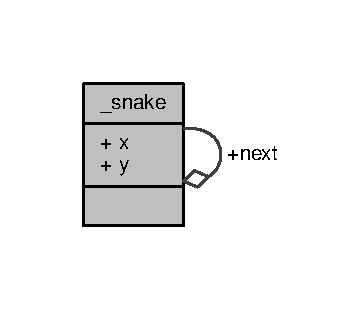
\includegraphics[width=174pt]{struct__snake__coll__graph}
\end{center}
\end{figure}
\subsection*{Attributs publics}
\begin{DoxyCompactItemize}
\item 
int \hyperlink{struct__snake_a58c7bdb2d495a8590718f12d2f7b4c20}{x}
\item 
int \hyperlink{struct__snake_a8739255d28f8c276b848dedda629a5d3}{y}
\item 
struct \hyperlink{struct__snake}{\+\_\+snake} $\ast$ \hyperlink{struct__snake_aa43aac7fd83d61bd422d927ffa889a69}{next}
\end{DoxyCompactItemize}


\subsection{Documentation des données membres}
\index{\+\_\+snake@{\+\_\+snake}!next@{next}}
\index{next@{next}!\+\_\+snake@{\+\_\+snake}}
\subsubsection[{\texorpdfstring{next}{next}}]{\setlength{\rightskip}{0pt plus 5cm}struct {\bf \+\_\+snake}$\ast$ \+\_\+snake\+::next}\hypertarget{struct__snake_aa43aac7fd83d61bd422d927ffa889a69}{}\label{struct__snake_aa43aac7fd83d61bd422d927ffa889a69}
\index{\+\_\+snake@{\+\_\+snake}!x@{x}}
\index{x@{x}!\+\_\+snake@{\+\_\+snake}}
\subsubsection[{\texorpdfstring{x}{x}}]{\setlength{\rightskip}{0pt plus 5cm}int \+\_\+snake\+::x}\hypertarget{struct__snake_a58c7bdb2d495a8590718f12d2f7b4c20}{}\label{struct__snake_a58c7bdb2d495a8590718f12d2f7b4c20}
\index{\+\_\+snake@{\+\_\+snake}!y@{y}}
\index{y@{y}!\+\_\+snake@{\+\_\+snake}}
\subsubsection[{\texorpdfstring{y}{y}}]{\setlength{\rightskip}{0pt plus 5cm}int \+\_\+snake\+::y}\hypertarget{struct__snake_a8739255d28f8c276b848dedda629a5d3}{}\label{struct__snake_a8739255d28f8c276b848dedda629a5d3}


La documentation de cette structure a été générée à partir du fichier suivant \+:\begin{DoxyCompactItemize}
\item 
I\+N\+C\+L\+U\+D\+E/\hyperlink{snakelib_8h}{snakelib.\+h}\end{DoxyCompactItemize}

\hypertarget{structboard}{}\section{Référence de la structure board}
\label{structboard}\index{board@{board}}


int $\ast$$\ast$array and int size tableau 2d et sa taille  




{\ttfamily \#include $<$snakelib.\+h$>$}



Graphe de collaboration de board\+:\nopagebreak
\begin{figure}[H]
\begin{center}
\leavevmode
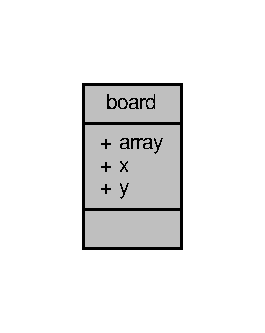
\includegraphics[width=127pt]{structboard__coll__graph}
\end{center}
\end{figure}
\subsection*{Attributs publics}
\begin{DoxyCompactItemize}
\item 
char $\ast$$\ast$ \hyperlink{structboard_a1d1e3a5155ec051a1e5a5e2d9de30e86}{array}
\item 
int \hyperlink{structboard_a45ad83890aed4b92ef175f0eb13cd1f3}{x}
\item 
int \hyperlink{structboard_a0a1685edc20c5b97527ccd4027d5f8eb}{y}
\end{DoxyCompactItemize}


\subsection{Description détaillée}
int $\ast$$\ast$array and int size tableau 2d et sa taille 

\subsection{Documentation des données membres}
\index{board@{board}!array@{array}}
\index{array@{array}!board@{board}}
\subsubsection[{\texorpdfstring{array}{array}}]{\setlength{\rightskip}{0pt plus 5cm}char$\ast$$\ast$ board\+::array}\hypertarget{structboard_a1d1e3a5155ec051a1e5a5e2d9de30e86}{}\label{structboard_a1d1e3a5155ec051a1e5a5e2d9de30e86}
\index{board@{board}!x@{x}}
\index{x@{x}!board@{board}}
\subsubsection[{\texorpdfstring{x}{x}}]{\setlength{\rightskip}{0pt plus 5cm}int board\+::x}\hypertarget{structboard_a45ad83890aed4b92ef175f0eb13cd1f3}{}\label{structboard_a45ad83890aed4b92ef175f0eb13cd1f3}
\index{board@{board}!y@{y}}
\index{y@{y}!board@{board}}
\subsubsection[{\texorpdfstring{y}{y}}]{\setlength{\rightskip}{0pt plus 5cm}int board\+::y}\hypertarget{structboard_a0a1685edc20c5b97527ccd4027d5f8eb}{}\label{structboard_a0a1685edc20c5b97527ccd4027d5f8eb}


La documentation de cette structure a été générée à partir du fichier suivant \+:\begin{DoxyCompactItemize}
\item 
I\+N\+C\+L\+U\+D\+E/\hyperlink{snakelib_8h}{snakelib.\+h}\end{DoxyCompactItemize}

\hypertarget{structsnake}{}\section{Référence de la structure snake}
\label{structsnake}\index{snake@{snake}}


linked list avec deux entiers x et y représente chaque élément du snake  




Graphe de collaboration de snake\+:\nopagebreak
\begin{figure}[H]
\begin{center}
\leavevmode
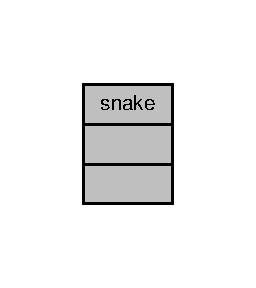
\includegraphics[width=123pt]{structsnake__coll__graph}
\end{center}
\end{figure}


\subsection{Description détaillée}
linked list avec deux entiers x et y représente chaque élément du snake 

La documentation de cette structure a été générée à partir du fichier suivant \+:\begin{DoxyCompactItemize}
\item 
I\+N\+C\+L\+U\+D\+E/\hyperlink{snakelib_8h}{snakelib.\+h}\end{DoxyCompactItemize}

\chapter{Documentation des fichiers}
\hypertarget{schlangalib_8h}{}\section{Référence du fichier I\+N\+C\+L\+U\+D\+E/schlangalib.h}
\label{schlangalib_8h}\index{I\+N\+C\+L\+U\+D\+E/schlangalib.\+h@{I\+N\+C\+L\+U\+D\+E/schlangalib.\+h}}
Ce graphe montre quels fichiers incluent directement ou indirectement ce fichier \+:\nopagebreak
\begin{figure}[H]
\begin{center}
\leavevmode
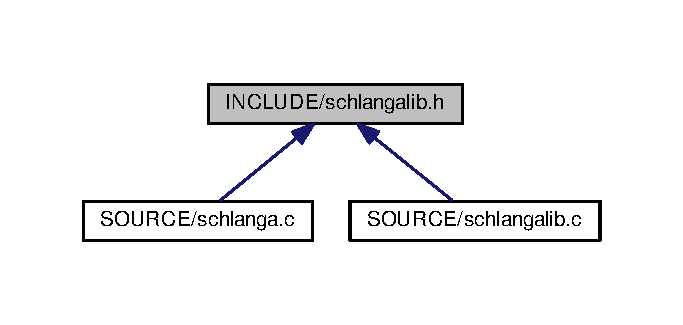
\includegraphics[width=328pt]{schlangalib_8h__dep__incl}
\end{center}
\end{figure}
\subsection*{Fonctions}
\begin{DoxyCompactItemize}
\item 
void \hyperlink{schlangalib_8h_a28adbac02fbdf8816543c25878bfd81d}{schlanga\+\_\+ia} (\hyperlink{structboard}{board} $\ast$\hyperlink{snake_8c_a20fdbd342281b7b5b77945c79d176b9f}{b}, const \hyperlink{structsnake}{snake} $\ast$\hyperlink{snake_8c_a71e92e96b65208605aca57598cc827f1}{s}, \hyperlink{structsnake}{snake} $\ast$\hyperlink{schlanga_8c_aa6fd7c53c9b79f5a6ccb6f73b383263c}{c}, int len)
\end{DoxyCompactItemize}


\subsection{Documentation des fonctions}
\index{schlangalib.\+h@{schlangalib.\+h}!schlanga\+\_\+ia@{schlanga\+\_\+ia}}
\index{schlanga\+\_\+ia@{schlanga\+\_\+ia}!schlangalib.\+h@{schlangalib.\+h}}
\subsubsection[{\texorpdfstring{schlanga\+\_\+ia(board $\ast$b, const snake $\ast$s, snake $\ast$c, int len)}{schlanga_ia(board *b, const snake *s, snake *c, int len)}}]{\setlength{\rightskip}{0pt plus 5cm}void schlanga\+\_\+ia (
\begin{DoxyParamCaption}
\item[{{\bf board} $\ast$}]{b, }
\item[{const {\bf snake} $\ast$}]{s, }
\item[{{\bf snake} $\ast$}]{c, }
\item[{int}]{len}
\end{DoxyParamCaption}
)}\hypertarget{schlangalib_8h_a28adbac02fbdf8816543c25878bfd81d}{}\label{schlangalib_8h_a28adbac02fbdf8816543c25878bfd81d}

\begin{DoxyCode}
437 \{
438     \textcolor{keyword}{static} \textcolor{keywordtype}{int} code = \hyperlink{schlangalib_8c_a012777a0d47b27fcae56ae35614459dd}{CODE\_NULL};
439     \textcolor{keyword}{static} \textcolor{keywordtype}{int} count = 0;
440     \textcolor{keyword}{static} \textcolor{keywordtype}{int} corner = 0;
441     \textcolor{keywordtype}{int} x\_board = 1;
442     \textcolor{keywordtype}{int} y\_board = 1;
443 
444     \textcolor{keywordtype}{int} dx\_board = b->\hyperlink{structboard_a45ad83890aed4b92ef175f0eb13cd1f3}{x} - 2;
445     \textcolor{keywordtype}{int} dy\_board = b->\hyperlink{structboard_a0a1685edc20c5b97527ccd4027d5f8eb}{y} - 2;
446 
447     \textcolor{keywordtype}{int} schlanga\_x = (*c)->x;
448     \textcolor{keywordtype}{int} schlanga\_y = (*c)->y;
449 
450     \textcolor{keywordtype}{int} schlanga\_dir\_x = (*c)->x - (*c)->next->x;
451     \textcolor{keywordtype}{int} schlanga\_dir\_y = (*c)->y - (*c)->next->y;
452 
453     \textcolor{keywordflow}{if}(\hyperlink{schlangalib_8c_a2655a50383ab9680d1a3a72ea9de562d}{schlanga\_next\_to}(b,s,c))
454     \{
455         code = \hyperlink{schlangalib_8c_a4baca3e22ae44aafc8a52b0768491cd3}{CODE\_NEXT\_TO};
456         \textcolor{keywordflow}{return};
457     \}
458     \textcolor{keywordflow}{if}(\hyperlink{schlangalib_8c_a08f1c27d2a4dd425ca550057e8856240}{schlanga\_corner}(b,c))
459     \{
460         code = \hyperlink{schlangalib_8c_a91640b78c7bda96c44c256a09f02e700}{CODE\_CORNER};
461         corner = len/2-2;
462         \textcolor{keywordflow}{return};
463     \}
464     \textcolor{keywordflow}{if}(corner)
465     \{
466         \textcolor{keywordflow}{if}(\hyperlink{schlangalib_8c_a4cb830baa18247d13d465075c869d1d7}{schlanga\_bow}(b,s,c))
467         \{
468             corner = 0;
469             code = \hyperlink{schlangalib_8c_aea2ff5b1ef8a3b2b9a385927575c9396}{CODE\_BOW};
470         \}
471         \textcolor{keywordflow}{else}
472         \{
473             \hyperlink{snakelib_8c_aa7c9d4fed2b3edb453a4501ba019dc00}{move}(b,c,\textcolor{charliteral}{'&'});
474             --corner;
475         \}
476         \textcolor{keywordflow}{return};
477     \}
478     \textcolor{keywordflow}{if}(code != \hyperlink{schlangalib_8c_acee163547d72d28d7cbb45de2c1cc1b9}{CODE\_WALL})
479     \{
480         \textcolor{keywordflow}{if}(\hyperlink{schlangalib_8c_a5b8413626002409e9465985272966386}{schlanga\_wall}(b,c))
481         \{
482             code = \hyperlink{schlangalib_8c_acee163547d72d28d7cbb45de2c1cc1b9}{CODE\_WALL};
483             \textcolor{keywordtype}{unsigned} \hyperlink{client_8c_a67668278838ab1eb0065ef9218c8de00}{m} = 0;
484             \textcolor{keywordflow}{if}(schlanga\_dir\_x == 0)
485             \{
486                 m = \hyperlink{schlangalib_8c_af3fdd05c8d6e18536c1f89f1814969d4}{min\_abs}(schlanga\_x - x\_board, schlanga\_x - dx\_board);
487             \}
488             \textcolor{keywordflow}{if}(schlanga\_dir\_y == 0)
489             \{
490                 m = \hyperlink{schlangalib_8c_af3fdd05c8d6e18536c1f89f1814969d4}{min\_abs}(schlanga\_y - y\_board, schlanga\_y - dy\_board);
491             \}
492             \textcolor{keywordflow}{if}(m != 0)
493             \{
494                 count = rand() % \hyperlink{client_8c_a67668278838ab1eb0065ef9218c8de00}{m};
495             \}
496             \textcolor{keywordflow}{return};
497         \}
498     \}
499     \textcolor{keywordflow}{else}
500     \{
501         \textcolor{keywordflow}{if}(count == 0)
502         \{
503             code = \hyperlink{schlangalib_8c_a012777a0d47b27fcae56ae35614459dd}{CODE\_NULL};
504         \}
505         \textcolor{keywordflow}{else}
506         \{
507             \textcolor{keywordflow}{if}(\hyperlink{schlangalib_8c_a4cb830baa18247d13d465075c869d1d7}{schlanga\_bow}(b,s,c))
508             \{
509                 code = \hyperlink{schlangalib_8c_aea2ff5b1ef8a3b2b9a385927575c9396}{CODE\_BOW};
510                 \textcolor{keywordflow}{return};
511             \}
512             \textcolor{keywordflow}{else}
513             \{
514                 \hyperlink{snakelib_8c_aa7c9d4fed2b3edb453a4501ba019dc00}{move}(b,c,\textcolor{charliteral}{'&'});
515                 --count;
516                 \textcolor{keywordflow}{return};
517             \}
518         \}
519     \}
520     \textcolor{keywordflow}{if}(\hyperlink{schlangalib_8c_a4cb830baa18247d13d465075c869d1d7}{schlanga\_bow}(b,s,c))
521     \{
522         code = \hyperlink{schlangalib_8c_aea2ff5b1ef8a3b2b9a385927575c9396}{CODE\_BOW};
523         \textcolor{keywordflow}{return};
524     \}
525     \hyperlink{snakelib_8c_aa7c9d4fed2b3edb453a4501ba019dc00}{move}(b,c,\textcolor{charliteral}{'&'});
526 \}\end{DoxyCode}


Voici le graphe d\textquotesingle{}appel pour cette fonction \+:\nopagebreak
\begin{figure}[H]
\begin{center}
\leavevmode
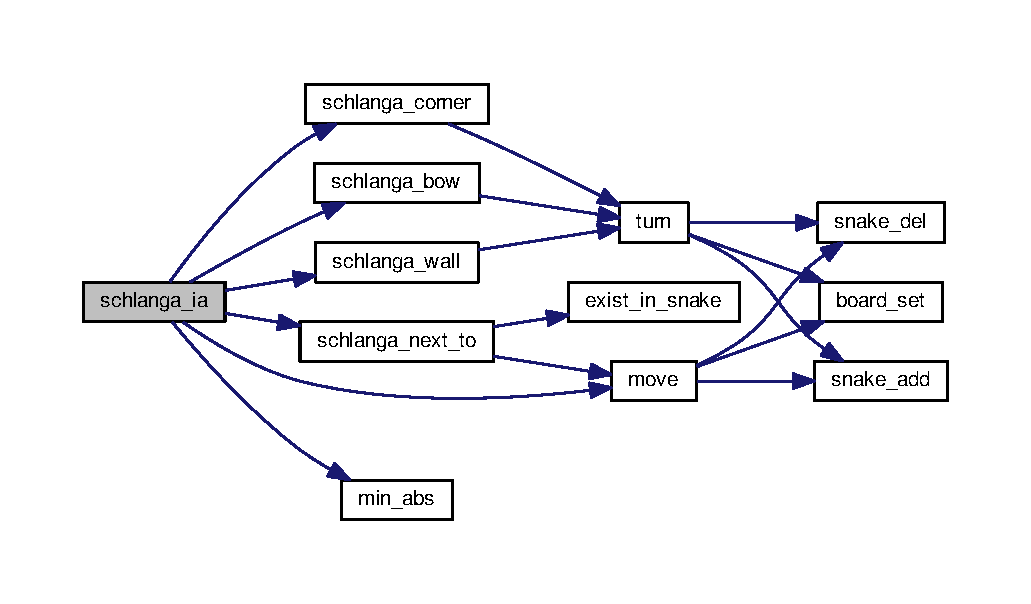
\includegraphics[width=350pt]{schlangalib_8h_a28adbac02fbdf8816543c25878bfd81d_cgraph}
\end{center}
\end{figure}




Voici le graphe des appelants de cette fonction \+:\nopagebreak
\begin{figure}[H]
\begin{center}
\leavevmode
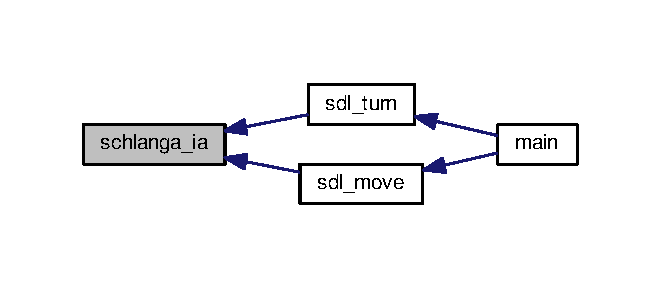
\includegraphics[width=317pt]{schlangalib_8h_a28adbac02fbdf8816543c25878bfd81d_icgraph}
\end{center}
\end{figure}



\hypertarget{snakelib_8h}{}\section{Référence du fichier I\+N\+C\+L\+U\+D\+E/snakelib.h}
\label{snakelib_8h}\index{I\+N\+C\+L\+U\+D\+E/snakelib.\+h@{I\+N\+C\+L\+U\+D\+E/snakelib.\+h}}
{\ttfamily \#include $<$sys/stat.\+h$>$}\\*
{\ttfamily \#include $<$stdio.\+h$>$}\\*
{\ttfamily \#include $<$stdlib.\+h$>$}\\*
{\ttfamily \#include $<$string.\+h$>$}\\*
{\ttfamily \#include $<$stdbool.\+h$>$}\\*
Graphe des dépendances par inclusion de snakelib.\+h\+:\nopagebreak
\begin{figure}[H]
\begin{center}
\leavevmode
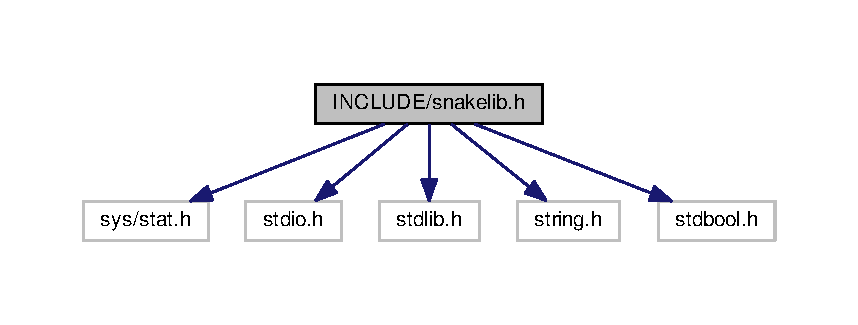
\includegraphics[width=350pt]{snakelib_8h__incl}
\end{center}
\end{figure}
Ce graphe montre quels fichiers incluent directement ou indirectement ce fichier \+:\nopagebreak
\begin{figure}[H]
\begin{center}
\leavevmode
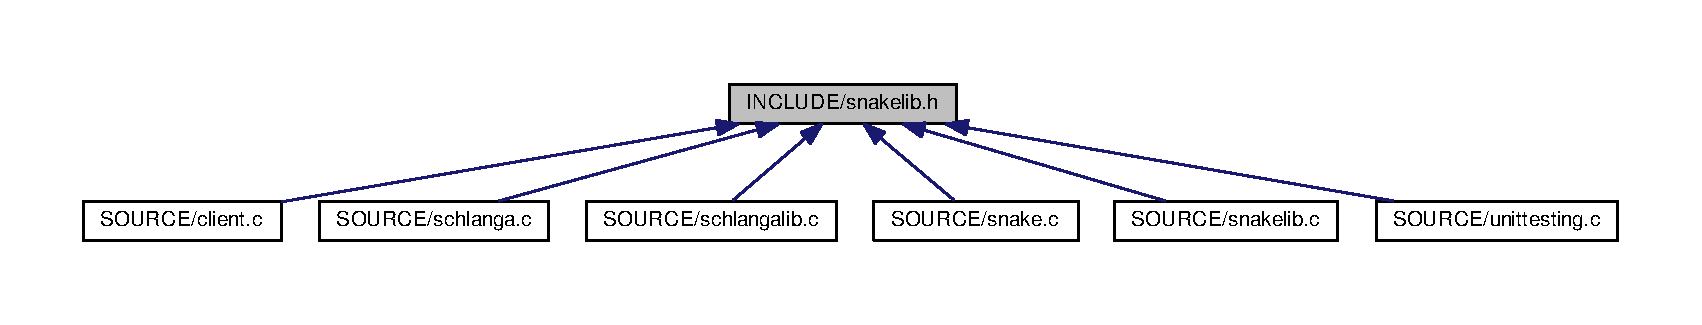
\includegraphics[width=350pt]{snakelib_8h__dep__incl}
\end{center}
\end{figure}
\subsection*{Classes}
\begin{DoxyCompactItemize}
\item 
struct \hyperlink{structboard}{board}
\begin{DoxyCompactList}\small\item\em int $\ast$$\ast$array and int size tableau 2d et sa taille \end{DoxyCompactList}\item 
struct \hyperlink{struct__snake}{\+\_\+snake}
\end{DoxyCompactItemize}
\subsection*{Définitions de type}
\begin{DoxyCompactItemize}
\item 
typedef struct \hyperlink{structboard}{board} \hyperlink{snakelib_8h_ad003b32f47ccbf4e9557f3541af47789}{board}
\item 
typedef struct \hyperlink{struct__snake}{\+\_\+snake} \hyperlink{snakelib_8h_a37a403a92b4650960d024935a50e67e9}{\+\_\+snake}
\item 
typedef \hyperlink{struct__snake}{\+\_\+snake} $\ast$ \hyperlink{snakelib_8h_aca379b653966f5fe335393b5a58e0aef}{snake}
\end{DoxyCompactItemize}
\subsection*{Fonctions}
\begin{DoxyCompactItemize}
\item 
int \hyperlink{snakelib_8h_ab6926a5a512798dea6aa52f5f15ab8ad}{board\+\_\+size\+\_\+x} (\hyperlink{structboard}{board} const $\ast$\hyperlink{snake_8c_a20fdbd342281b7b5b77945c79d176b9f}{b})
\begin{DoxyCompactList}\small\item\em taille x du plateau \end{DoxyCompactList}\item 
int \hyperlink{snakelib_8h_a01be021996158cf01e830b56e41be904}{board\+\_\+size\+\_\+y} (\hyperlink{structboard}{board} const $\ast$\hyperlink{snake_8c_a20fdbd342281b7b5b77945c79d176b9f}{b})
\item 
\hyperlink{structboard}{board} \hyperlink{snakelib_8h_a9625331c000178d2cf90ef40d2a8fbf7}{board\+\_\+init} (int x, int y)
\item 
void \hyperlink{snakelib_8h_a12954721537f652c82e9cf23c1bfb0c3}{board\+\_\+set} (\hyperlink{structboard}{board} $\ast$brdin, int x, int y, char value)
\item 
char \hyperlink{snakelib_8h_ae49b60c78ec9b92e770c8eace9520447}{board\+\_\+get} (\hyperlink{structboard}{board} const $\ast$brdin, int x, int y)
\begin{DoxyCompactList}\small\item\em return la valeur \end{DoxyCompactList}\item 
void \hyperlink{snakelib_8h_a223ea5e585467eee652b6b3b7a59e0c9}{board\+\_\+free} (\hyperlink{structboard}{board} $\ast$brdin)
\begin{DoxyCompactList}\small\item\em liberer la memoire occupé par un plateau \end{DoxyCompactList}\item 
void \hyperlink{snakelib_8h_a34e4ffa89cbd5062286074398f897bcf}{board\+\_\+print} (const \hyperlink{structboard}{board} $\ast$brdin)
\begin{DoxyCompactList}\small\item\em pour afficher un plateau \end{DoxyCompactList}\item 
void \hyperlink{snakelib_8h_aa228e2d2337022d7cf56c813b9540166}{board\+\_\+pxmap} (const \hyperlink{structboard}{board} $\ast$brdin, char $\ast$foldername, int filename, int zoom)
\begin{DoxyCompactList}\small\item\em créer une image ppm du tableau pour mieux voir et interpreter nos fonctions de teste \end{DoxyCompactList}\item 
void \hyperlink{snakelib_8h_a17492ac4841b98e25c682f9ff358ea2c}{snake\+\_\+add} (\hyperlink{structsnake}{snake} $\ast$snkin, int x, int y)
\begin{DoxyCompactList}\small\item\em un snake est équivalent à une file d\textquotesingle{}attente (F\+I\+FO « first in, first out »), cette fonction permet d\textquotesingle{}ajouter à l\textquotesingle{}entête de la liste \end{DoxyCompactList}\item 
void \hyperlink{snakelib_8h_a6b2f097d4deefee8b8f8d809691f44ce}{snake\+\_\+addl} (\hyperlink{structsnake}{snake} $\ast$snkin, int x, int y)
\item 
void \hyperlink{snakelib_8h_a9f15dca26b0f46aae4e1e5cf30db9ab9}{snake\+\_\+getl} (\hyperlink{structsnake}{snake} $\ast$snkin, int $\ast$x, int $\ast$y)
\item 
void \hyperlink{snakelib_8h_aa723bfe337f8108975b8d36292b422d1}{snake\+\_\+del} (\hyperlink{structsnake}{snake} $\ast$snkin, int $\ast$x, int $\ast$y)
\begin{DoxyCompactList}\small\item\em un snake est équivalent à une file d\textquotesingle{}attente (F\+I\+FO « first in, first out »), cette fonction permet de supprimer au queue de la liste \end{DoxyCompactList}\item 
void \hyperlink{snakelib_8h_ae2b728ff11f9b12d88715ddef95639c9}{snake\+\_\+free} (\hyperlink{structsnake}{snake} $\ast$snkin)
\begin{DoxyCompactList}\small\item\em libérer la mémoire \end{DoxyCompactList}\item 
void \hyperlink{snakelib_8h_a08f653b84e023db977cc57ff5fc8debf}{snake\+\_\+print} (const \hyperlink{structsnake}{snake} $\ast$snkin)
\item 
void \hyperlink{snakelib_8h_aa7c9d4fed2b3edb453a4501ba019dc00}{move} (\hyperlink{structboard}{board} $\ast$brdin, \hyperlink{structsnake}{snake} $\ast$snkin, char id)
\item 
void \hyperlink{snakelib_8h_afa428ecb4385e08a82520bec11bafe36}{turn} (\hyperlink{structboard}{board} $\ast$brdin, \hyperlink{structsnake}{snake} $\ast$snkin, int drctn, char id)
\item 
void \hyperlink{snakelib_8h_ac696fcc76930ea0badb2f263dd479c93}{snake\+\_\+init} (\hyperlink{structboard}{board} $\ast$brdin, \hyperlink{structsnake}{snake} $\ast$snkin, int len, char id)
\begin{DoxyCompactList}\small\item\em init a snake \end{DoxyCompactList}\item 
bool \hyperlink{snakelib_8h_ab96735ae82693727289ffe22fc940235}{choc\+\_\+snake} (\hyperlink{structsnake}{snake} const $\ast$s1, \hyperlink{structsnake}{snake} const $\ast$s2)
\begin{DoxyCompactList}\small\item\em test choc entre deux snake \end{DoxyCompactList}\item 
bool \hyperlink{snakelib_8h_ab72d8c937b91594a9c27b30c05a08a75}{choc\+\_\+sc} (\hyperlink{structsnake}{snake} const $\ast$s1, \hyperlink{structsnake}{snake} const $\ast$s2)
\item 
bool \hyperlink{snakelib_8h_a50fa8a047abfa006a3371a94809e72c4}{choc\+\_\+wall} (\hyperlink{structboard}{board} const $\ast$\hyperlink{snake_8c_a20fdbd342281b7b5b77945c79d176b9f}{b}, \hyperlink{structsnake}{snake} const $\ast$\hyperlink{snake_8c_a71e92e96b65208605aca57598cc827f1}{s})
\begin{DoxyCompactList}\small\item\em test choc snake contre le mur \end{DoxyCompactList}\item 
void \hyperlink{snakelib_8h_ab4819fcf1df66683feca8ad73abd89dd}{board\+\_\+apple} (\hyperlink{structboard}{board} $\ast$\hyperlink{snake_8c_a20fdbd342281b7b5b77945c79d176b9f}{b}, int $\ast$x, int $\ast$y)
\item 
bool \hyperlink{snakelib_8h_a9c77869dc19e2c9bc443ab997aad1f4f}{snake\+\_\+apple} (\hyperlink{structsnake}{snake} const $\ast$\hyperlink{snake_8c_a71e92e96b65208605aca57598cc827f1}{s}, int $\ast$x, int $\ast$y)
\end{DoxyCompactItemize}


\subsection{Documentation des définitions de type}
\index{snakelib.\+h@{snakelib.\+h}!\+\_\+snake@{\+\_\+snake}}
\index{\+\_\+snake@{\+\_\+snake}!snakelib.\+h@{snakelib.\+h}}
\subsubsection[{\texorpdfstring{\+\_\+snake}{_snake}}]{\setlength{\rightskip}{0pt plus 5cm}typedef struct {\bf \+\_\+snake} {\bf \+\_\+snake}}\hypertarget{snakelib_8h_a37a403a92b4650960d024935a50e67e9}{}\label{snakelib_8h_a37a403a92b4650960d024935a50e67e9}
\index{snakelib.\+h@{snakelib.\+h}!board@{board}}
\index{board@{board}!snakelib.\+h@{snakelib.\+h}}
\subsubsection[{\texorpdfstring{board}{board}}]{\setlength{\rightskip}{0pt plus 5cm}typedef struct {\bf board} {\bf board}}\hypertarget{snakelib_8h_ad003b32f47ccbf4e9557f3541af47789}{}\label{snakelib_8h_ad003b32f47ccbf4e9557f3541af47789}
\index{snakelib.\+h@{snakelib.\+h}!snake@{snake}}
\index{snake@{snake}!snakelib.\+h@{snakelib.\+h}}
\subsubsection[{\texorpdfstring{snake}{snake}}]{\setlength{\rightskip}{0pt plus 5cm}typedef {\bf \+\_\+snake}$\ast$ {\bf snake}}\hypertarget{snakelib_8h_aca379b653966f5fe335393b5a58e0aef}{}\label{snakelib_8h_aca379b653966f5fe335393b5a58e0aef}


\subsection{Documentation des fonctions}
\index{snakelib.\+h@{snakelib.\+h}!board\+\_\+apple@{board\+\_\+apple}}
\index{board\+\_\+apple@{board\+\_\+apple}!snakelib.\+h@{snakelib.\+h}}
\subsubsection[{\texorpdfstring{board\+\_\+apple(board $\ast$b, int $\ast$x, int $\ast$y)}{board_apple(board *b, int *x, int *y)}}]{\setlength{\rightskip}{0pt plus 5cm}void board\+\_\+apple (
\begin{DoxyParamCaption}
\item[{{\bf board} $\ast$}]{b, }
\item[{int $\ast$}]{x, }
\item[{int $\ast$}]{y}
\end{DoxyParamCaption}
)}\hypertarget{snakelib_8h_ab4819fcf1df66683feca8ad73abd89dd}{}\label{snakelib_8h_ab4819fcf1df66683feca8ad73abd89dd}

\begin{DoxyCode}
512 \{
513     \textcolor{keywordtype}{bool} \hyperlink{client_8c_af6f0bd3dc13317f895c91323c25c2b8f}{t} = \textcolor{keyword}{true};
514     \textcolor{keywordflow}{while}(t)
515     \{
516             *x = \hyperlink{snakelib_8c_a31044302280c0ec9eca89286f81127af}{rand\_a\_b}(1, b->\hyperlink{structboard_a45ad83890aed4b92ef175f0eb13cd1f3}{x}-2);
517             *y = \hyperlink{snakelib_8c_a31044302280c0ec9eca89286f81127af}{rand\_a\_b}(1, b->\hyperlink{structboard_a0a1685edc20c5b97527ccd4027d5f8eb}{y}-2);
518             \textcolor{keywordflow}{if}(\hyperlink{snakelib_8c_ae49b60c78ec9b92e770c8eace9520447}{board\_get}(b,*x,*y) == \textcolor{charliteral}{' '})
519             \{
520                 \hyperlink{snakelib_8c_a12954721537f652c82e9cf23c1bfb0c3}{board\_set}(b,*x,*y,\textcolor{charliteral}{'$'});
521                 t = \textcolor{keyword}{false};
522             \}
523     \}
524 \}
\end{DoxyCode}


Voici le graphe d\textquotesingle{}appel pour cette fonction \+:\nopagebreak
\begin{figure}[H]
\begin{center}
\leavevmode
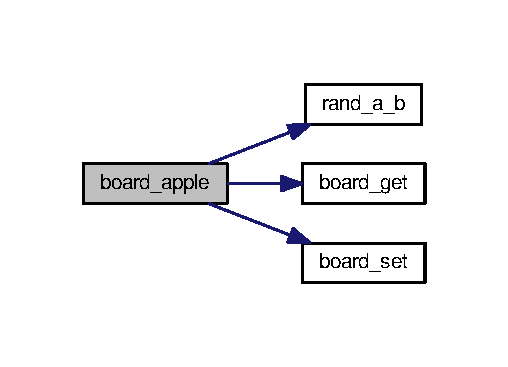
\includegraphics[width=244pt]{snakelib_8h_ab4819fcf1df66683feca8ad73abd89dd_cgraph}
\end{center}
\end{figure}




Voici le graphe des appelants de cette fonction \+:\nopagebreak
\begin{figure}[H]
\begin{center}
\leavevmode
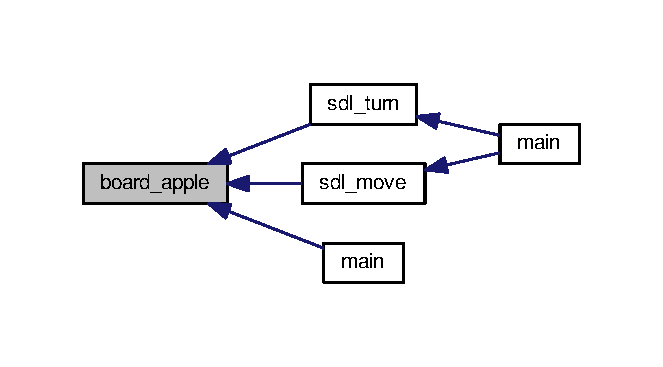
\includegraphics[width=318pt]{snakelib_8h_ab4819fcf1df66683feca8ad73abd89dd_icgraph}
\end{center}
\end{figure}


\index{snakelib.\+h@{snakelib.\+h}!board\+\_\+free@{board\+\_\+free}}
\index{board\+\_\+free@{board\+\_\+free}!snakelib.\+h@{snakelib.\+h}}
\subsubsection[{\texorpdfstring{board\+\_\+free(board $\ast$brdin)}{board_free(board *brdin)}}]{\setlength{\rightskip}{0pt plus 5cm}void board\+\_\+free (
\begin{DoxyParamCaption}
\item[{{\bf board} $\ast$}]{brdin}
\end{DoxyParamCaption}
)}\hypertarget{snakelib_8h_a223ea5e585467eee652b6b3b7a59e0c9}{}\label{snakelib_8h_a223ea5e585467eee652b6b3b7a59e0c9}


liberer la memoire occupé par un plateau 


\begin{DoxyParams}{Paramètres}
{\em adresse} & du plateau à libérer \\
\hline
\end{DoxyParams}
\begin{DoxyReturn}{Renvoie}
une fonction de type void 
\end{DoxyReturn}

\begin{DoxyCode}
91 \{
92     \textcolor{keywordtype}{int} i;
93     
94     \textcolor{keywordflow}{for}(i = 0; i < brdin->\hyperlink{structboard_a0a1685edc20c5b97527ccd4027d5f8eb}{y} ; i++)
95     \{
96         free(brdin->\hyperlink{structboard_a1d1e3a5155ec051a1e5a5e2d9de30e86}{array}[i]);
97         brdin->\hyperlink{structboard_a1d1e3a5155ec051a1e5a5e2d9de30e86}{array}[i] = NULL;
98     \}
99     
100     free(brdin->\hyperlink{structboard_a1d1e3a5155ec051a1e5a5e2d9de30e86}{array});
101     brdin->\hyperlink{structboard_a1d1e3a5155ec051a1e5a5e2d9de30e86}{array} = NULL;
102 \}
\end{DoxyCode}


Voici le graphe des appelants de cette fonction \+:\nopagebreak
\begin{figure}[H]
\begin{center}
\leavevmode
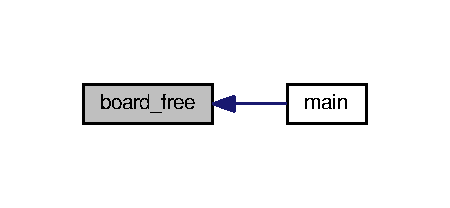
\includegraphics[width=216pt]{snakelib_8h_a223ea5e585467eee652b6b3b7a59e0c9_icgraph}
\end{center}
\end{figure}


\index{snakelib.\+h@{snakelib.\+h}!board\+\_\+get@{board\+\_\+get}}
\index{board\+\_\+get@{board\+\_\+get}!snakelib.\+h@{snakelib.\+h}}
\subsubsection[{\texorpdfstring{board\+\_\+get(board const $\ast$brdin, int x, int y)}{board_get(board const *brdin, int x, int y)}}]{\setlength{\rightskip}{0pt plus 5cm}char board\+\_\+get (
\begin{DoxyParamCaption}
\item[{{\bf board} const $\ast$}]{brdin, }
\item[{int}]{x, }
\item[{int}]{y}
\end{DoxyParamCaption}
)}\hypertarget{snakelib_8h_ae49b60c78ec9b92e770c8eace9520447}{}\label{snakelib_8h_ae49b60c78ec9b92e770c8eace9520447}


return la valeur 


\begin{DoxyParams}{Paramètres}
{\em adresse} & d\textquotesingle{}un plateau pour accéder et modifier simplement ses variables \\
\hline
{\em x} & et y la case à visiter \\
\hline
\end{DoxyParams}
\begin{DoxyReturn}{Renvoie}
char la valueur du point (x,y) 
\end{DoxyReturn}

\begin{DoxyCode}
70 \{
71     \textcolor{keywordflow}{return} brdin->array[y][x];
72 \}
\end{DoxyCode}


Voici le graphe des appelants de cette fonction \+:\nopagebreak
\begin{figure}[H]
\begin{center}
\leavevmode
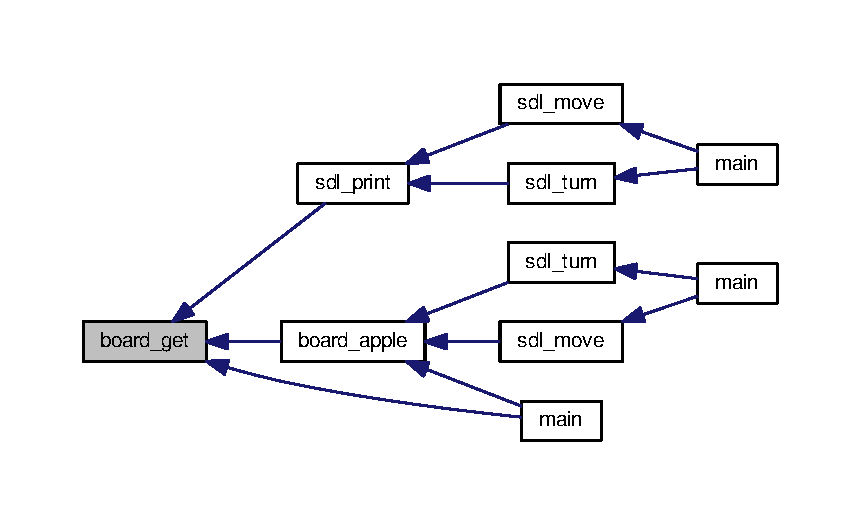
\includegraphics[width=350pt]{snakelib_8h_ae49b60c78ec9b92e770c8eace9520447_icgraph}
\end{center}
\end{figure}


\index{snakelib.\+h@{snakelib.\+h}!board\+\_\+init@{board\+\_\+init}}
\index{board\+\_\+init@{board\+\_\+init}!snakelib.\+h@{snakelib.\+h}}
\subsubsection[{\texorpdfstring{board\+\_\+init(int x, int y)}{board_init(int x, int y)}}]{\setlength{\rightskip}{0pt plus 5cm}{\bf board} board\+\_\+init (
\begin{DoxyParamCaption}
\item[{int}]{x, }
\item[{int}]{y}
\end{DoxyParamCaption}
)}\hypertarget{snakelib_8h_a9625331c000178d2cf90ef40d2a8fbf7}{}\label{snakelib_8h_a9625331c000178d2cf90ef40d2a8fbf7}
borders values is \textquotesingle{}\#\textquotesingle{}. 
\begin{DoxyCode}
22 \{
23     \hyperlink{structboard}{board} brdout;
24     
25     brdout.\hyperlink{structboard_a45ad83890aed4b92ef175f0eb13cd1f3}{x} = x;
26     brdout.\hyperlink{structboard_a0a1685edc20c5b97527ccd4027d5f8eb}{y} = y;
27     
28     \textcolor{keywordtype}{int} i, j;
29     
30     brdout.\hyperlink{structboard_a1d1e3a5155ec051a1e5a5e2d9de30e86}{array}=malloc(y*\textcolor{keyword}{sizeof}(\textcolor{keywordtype}{char}*));
31     \textcolor{keywordflow}{for}(i = 0; i < y; i++)
32         brdout.\hyperlink{structboard_a1d1e3a5155ec051a1e5a5e2d9de30e86}{array}[i] = malloc(x*\textcolor{keyword}{sizeof}(\textcolor{keywordtype}{int}));
33         
34 
36     \textcolor{keywordflow}{for}(i = 0; i < x; i++)
37     \{
38         brdout.\hyperlink{structboard_a1d1e3a5155ec051a1e5a5e2d9de30e86}{array}[0][i] = \textcolor{charliteral}{'#'};
39         brdout.\hyperlink{structboard_a1d1e3a5155ec051a1e5a5e2d9de30e86}{array}[y-1][i] = \textcolor{charliteral}{'#'};
40     \}
41     \textcolor{keywordflow}{for}(i = 0;i < y; i++)
42     \{
43         brdout.\hyperlink{structboard_a1d1e3a5155ec051a1e5a5e2d9de30e86}{array}[i][0] = \textcolor{charliteral}{'#'};
44         brdout.\hyperlink{structboard_a1d1e3a5155ec051a1e5a5e2d9de30e86}{array}[i][x-1] = \textcolor{charliteral}{'#'};
45     \}
46     
47     \textcolor{keywordflow}{for}(i = 1; i < y-1; i++)
48         \textcolor{keywordflow}{for}(j = 1; j < x-1; j++)
49             brdout.\hyperlink{structboard_a1d1e3a5155ec051a1e5a5e2d9de30e86}{array}[i][j] = \textcolor{charliteral}{' '};
50             
51     \textcolor{keywordflow}{return} brdout;
52 \}
\end{DoxyCode}


Voici le graphe des appelants de cette fonction \+:\nopagebreak
\begin{figure}[H]
\begin{center}
\leavevmode
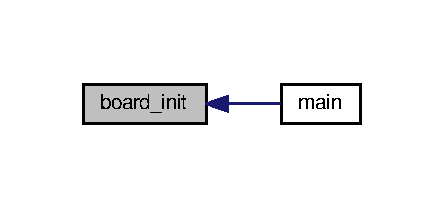
\includegraphics[width=213pt]{snakelib_8h_a9625331c000178d2cf90ef40d2a8fbf7_icgraph}
\end{center}
\end{figure}


\index{snakelib.\+h@{snakelib.\+h}!board\+\_\+print@{board\+\_\+print}}
\index{board\+\_\+print@{board\+\_\+print}!snakelib.\+h@{snakelib.\+h}}
\subsubsection[{\texorpdfstring{board\+\_\+print(const board $\ast$brdin)}{board_print(const board *brdin)}}]{\setlength{\rightskip}{0pt plus 5cm}void board\+\_\+print (
\begin{DoxyParamCaption}
\item[{const {\bf board} $\ast$}]{brdin}
\end{DoxyParamCaption}
)}\hypertarget{snakelib_8h_a34e4ffa89cbd5062286074398f897bcf}{}\label{snakelib_8h_a34e4ffa89cbd5062286074398f897bcf}


pour afficher un plateau 


\begin{DoxyParams}{Paramètres}
{\em une} & adresse d\textquotesingle{}un plateau concéder constant (droit que pour la lecture) pour éviter de copier le plateau \\
\hline
\end{DoxyParams}
\begin{DoxyReturn}{Renvoie}
une fonction de type void 
\end{DoxyReturn}

\begin{DoxyCode}
113 \{
114     \textcolor{keywordtype}{int} i,j;
115     \textcolor{comment}{/* traversing 2d-array */}
116     \textcolor{keywordflow}{for}(i=0 ; i < brdin->\hyperlink{structboard_a0a1685edc20c5b97527ccd4027d5f8eb}{y}; i++)
117     \{
118         \textcolor{keywordflow}{for}(j=0 ;j < brdin->\hyperlink{structboard_a45ad83890aed4b92ef175f0eb13cd1f3}{x}; j++)
119         \{
120             printf(\textcolor{stringliteral}{"%c"}, brdin->\hyperlink{structboard_a1d1e3a5155ec051a1e5a5e2d9de30e86}{array}[i][j]);
121         \}
122         printf(\textcolor{stringliteral}{"\(\backslash\)n"});
123     \}
124 \}
\end{DoxyCode}


Voici le graphe des appelants de cette fonction \+:\nopagebreak
\begin{figure}[H]
\begin{center}
\leavevmode
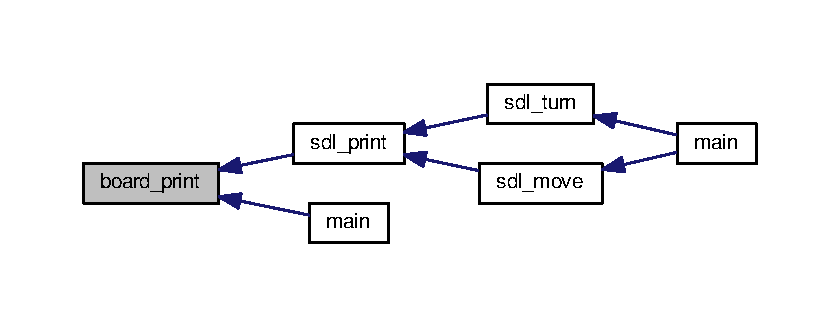
\includegraphics[width=350pt]{snakelib_8h_a34e4ffa89cbd5062286074398f897bcf_icgraph}
\end{center}
\end{figure}


\index{snakelib.\+h@{snakelib.\+h}!board\+\_\+pxmap@{board\+\_\+pxmap}}
\index{board\+\_\+pxmap@{board\+\_\+pxmap}!snakelib.\+h@{snakelib.\+h}}
\subsubsection[{\texorpdfstring{board\+\_\+pxmap(const board $\ast$brdin, char $\ast$foldername, int filename, int zoom)}{board_pxmap(const board *brdin, char *foldername, int filename, int zoom)}}]{\setlength{\rightskip}{0pt plus 5cm}void board\+\_\+pxmap (
\begin{DoxyParamCaption}
\item[{const {\bf board} $\ast$}]{brdin, }
\item[{char $\ast$}]{foldername, }
\item[{int}]{filename, }
\item[{int}]{zoom}
\end{DoxyParamCaption}
)}\hypertarget{snakelib_8h_aa228e2d2337022d7cf56c813b9540166}{}\label{snakelib_8h_aa228e2d2337022d7cf56c813b9540166}


créer une image ppm du tableau pour mieux voir et interpreter nos fonctions de teste 


\begin{DoxyParams}{Paramètres}
{\em une} & adresse d\textquotesingle{}un plateau concéder constant (droit que pour la lecture) pour éviter de copier le plateau \\
\hline
{\em char$\ast$} & foldername\+: donner un nom au dossier créé \\
\hline
{\em int} & filename\+: numero de la map \\
\hline
{\em int} & zoom\+: pour definir le zoom appliqué a la map ( taille d\textquotesingle{}une case en px = zoom $\ast$ 1px ) \\
\hline
\end{DoxyParams}
\begin{DoxyReturn}{Renvoie}
une fonction de type void 
\end{DoxyReturn}
le dossier n\textquotesingle{}existe pas 
\begin{DoxyCode}
141 \{
142     \textcolor{keyword}{struct }stat dir\_stat;
143     \textcolor{keywordflow}{if}(stat(foldername, &dir\_stat) < 0)
145         mkdir(foldername, S\_IRWXU);
146     
147     
148     \textcolor{keywordtype}{char} ffilename[strlen(foldername) + 7];
149     sprintf(ffilename, \textcolor{stringliteral}{"%s/%d.ppm"}, foldername, filename);
150     FILE* fdout = fopen( ffilename, \textcolor{stringliteral}{"w"});
151     fprintf(fdout, \textcolor{stringliteral}{"P3\(\backslash\)n%d %d\(\backslash\)n255\(\backslash\)n"}, brdin->\hyperlink{structboard_a0a1685edc20c5b97527ccd4027d5f8eb}{y} * zoom,\(\backslash\)
152             brdin->\hyperlink{structboard_a45ad83890aed4b92ef175f0eb13cd1f3}{x} * zoom);
153             
154     
155     \textcolor{keywordtype}{int} i,j,\hyperlink{client_8c_a70893b9fd599f8c9ed3ed00c52eba44a}{l},k;
156     \textcolor{comment}{/* traversing 2d-array */}
157     \textcolor{keywordflow}{for}(i = 0; i < brdin->\hyperlink{structboard_a0a1685edc20c5b97527ccd4027d5f8eb}{y}; i++)
158     \{
159      \textcolor{keywordflow}{for}(l = 0; l < zoom; l++)
160      \{
161       \textcolor{keywordflow}{for}(j = 0; j < brdin->\hyperlink{structboard_a45ad83890aed4b92ef175f0eb13cd1f3}{x}; j++)
162       \{
163        \textcolor{keywordflow}{for}(k = 0; k < zoom; k++)
164        \{
165          \textcolor{keywordflow}{if}(brdin->\hyperlink{structboard_a1d1e3a5155ec051a1e5a5e2d9de30e86}{array}[i][j] == \textcolor{charliteral}{' '})
166           fprintf(fdout,\textcolor{stringliteral}{"175 175 175 "});
167          \textcolor{keywordflow}{else} \textcolor{keywordflow}{if}(brdin->\hyperlink{structboard_a1d1e3a5155ec051a1e5a5e2d9de30e86}{array}[i][j] == \textcolor{charliteral}{'#'})
168           fprintf(fdout,\textcolor{stringliteral}{"48 48 48 "});
169          \textcolor{keywordflow}{else} \textcolor{keywordflow}{if}(brdin->\hyperlink{structboard_a1d1e3a5155ec051a1e5a5e2d9de30e86}{array}[i][j] == \textcolor{charliteral}{'@'})
170           fprintf(fdout,\textcolor{stringliteral}{"110 11 20 "});
171        \}
172       \}
173       fprintf(fdout, \textcolor{stringliteral}{"\(\backslash\)n"});
174      \}
175      fprintf(fdout, \textcolor{stringliteral}{"\(\backslash\)n"});
176     \}
177     fclose(fdout);
178     
179     
180 \}
\end{DoxyCode}
\index{snakelib.\+h@{snakelib.\+h}!board\+\_\+set@{board\+\_\+set}}
\index{board\+\_\+set@{board\+\_\+set}!snakelib.\+h@{snakelib.\+h}}
\subsubsection[{\texorpdfstring{board\+\_\+set(board $\ast$brdin, int x, int y, char value)}{board_set(board *brdin, int x, int y, char value)}}]{\setlength{\rightskip}{0pt plus 5cm}void board\+\_\+set (
\begin{DoxyParamCaption}
\item[{{\bf board} $\ast$}]{brdin, }
\item[{int}]{x, }
\item[{int}]{y, }
\item[{char}]{value}
\end{DoxyParamCaption}
)}\hypertarget{snakelib_8h_a12954721537f652c82e9cf23c1bfb0c3}{}\label{snakelib_8h_a12954721537f652c82e9cf23c1bfb0c3}

\begin{DoxyCode}
65 \{
66     brdin->\hyperlink{structboard_a1d1e3a5155ec051a1e5a5e2d9de30e86}{array}[y][x] = value;
67 \}
\end{DoxyCode}


Voici le graphe des appelants de cette fonction \+:\nopagebreak
\begin{figure}[H]
\begin{center}
\leavevmode
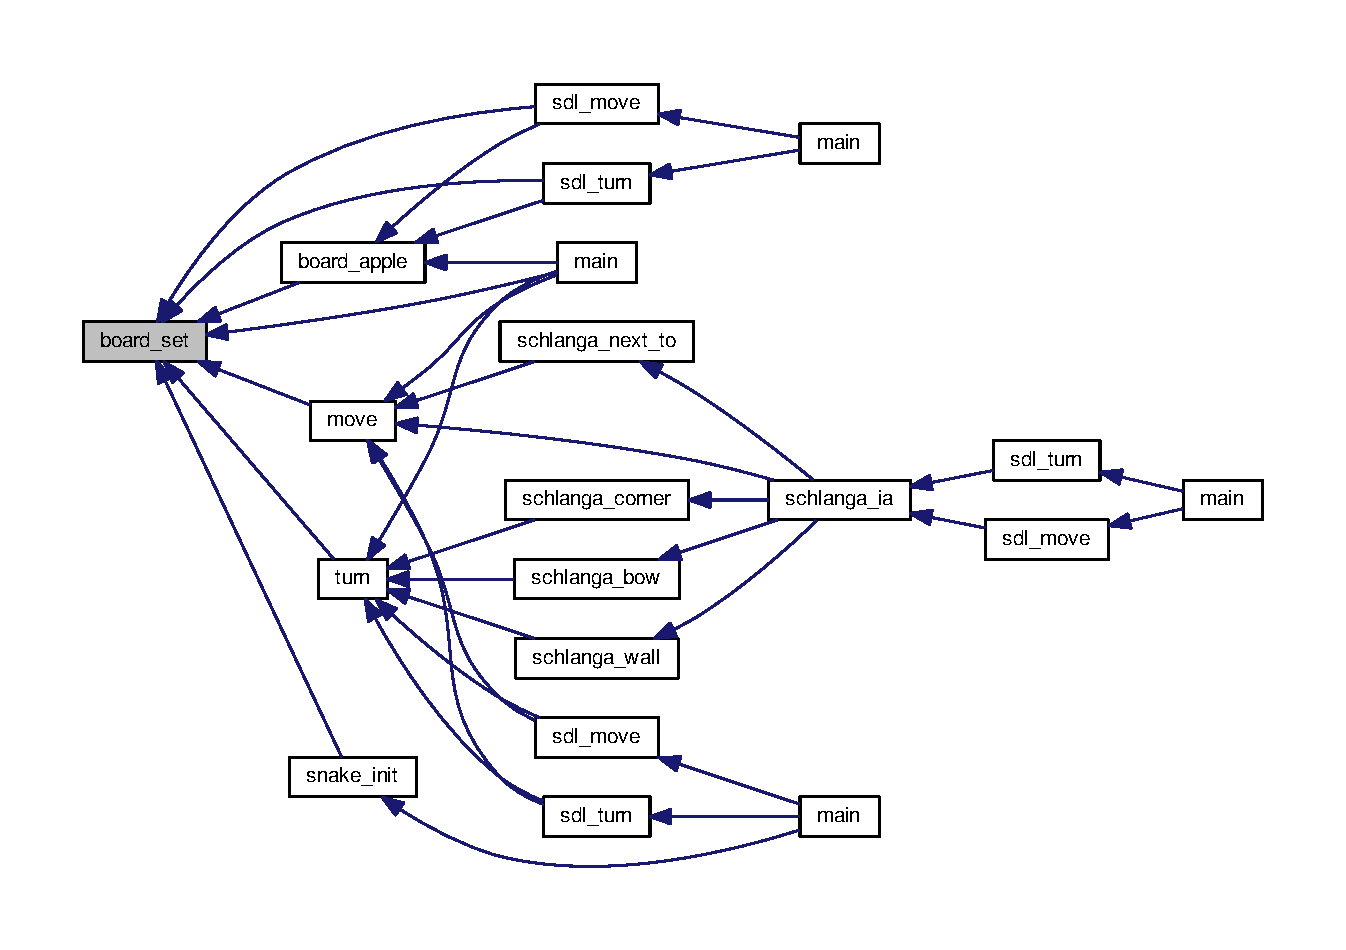
\includegraphics[width=350pt]{snakelib_8h_a12954721537f652c82e9cf23c1bfb0c3_icgraph}
\end{center}
\end{figure}


\index{snakelib.\+h@{snakelib.\+h}!board\+\_\+size\+\_\+x@{board\+\_\+size\+\_\+x}}
\index{board\+\_\+size\+\_\+x@{board\+\_\+size\+\_\+x}!snakelib.\+h@{snakelib.\+h}}
\subsubsection[{\texorpdfstring{board\+\_\+size\+\_\+x(board const $\ast$b)}{board_size_x(board const *b)}}]{\setlength{\rightskip}{0pt plus 5cm}int board\+\_\+size\+\_\+x (
\begin{DoxyParamCaption}
\item[{{\bf board} const $\ast$}]{b}
\end{DoxyParamCaption}
)}\hypertarget{snakelib_8h_ab6926a5a512798dea6aa52f5f15ab8ad}{}\label{snakelib_8h_ab6926a5a512798dea6aa52f5f15ab8ad}


taille x du plateau 

taille y du plateau


\begin{DoxyParams}{Paramètres}
{\em adresse} & du plateau \\
\hline
\end{DoxyParams}

\begin{DoxyCode}
75 \{
76     \textcolor{keywordflow}{return} \hyperlink{client_8c_a20fdbd342281b7b5b77945c79d176b9f}{b}->\hyperlink{structboard_a45ad83890aed4b92ef175f0eb13cd1f3}{x};
77 \}
\end{DoxyCode}


Voici le graphe des appelants de cette fonction \+:\nopagebreak
\begin{figure}[H]
\begin{center}
\leavevmode
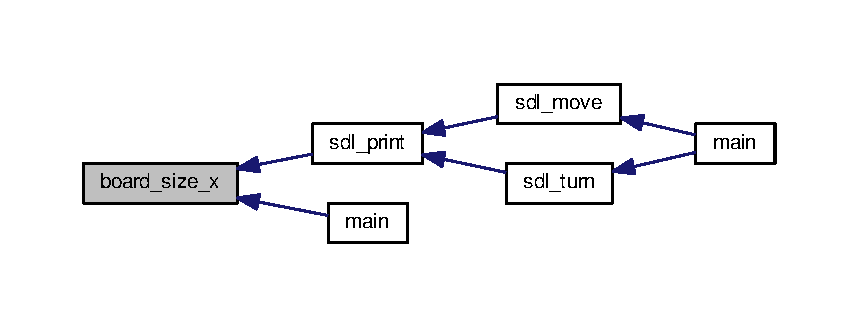
\includegraphics[width=350pt]{snakelib_8h_ab6926a5a512798dea6aa52f5f15ab8ad_icgraph}
\end{center}
\end{figure}


\index{snakelib.\+h@{snakelib.\+h}!board\+\_\+size\+\_\+y@{board\+\_\+size\+\_\+y}}
\index{board\+\_\+size\+\_\+y@{board\+\_\+size\+\_\+y}!snakelib.\+h@{snakelib.\+h}}
\subsubsection[{\texorpdfstring{board\+\_\+size\+\_\+y(board const $\ast$b)}{board_size_y(board const *b)}}]{\setlength{\rightskip}{0pt plus 5cm}int board\+\_\+size\+\_\+y (
\begin{DoxyParamCaption}
\item[{{\bf board} const $\ast$}]{b}
\end{DoxyParamCaption}
)}\hypertarget{snakelib_8h_a01be021996158cf01e830b56e41be904}{}\label{snakelib_8h_a01be021996158cf01e830b56e41be904}

\begin{DoxyCode}
80 \{
81     \textcolor{keywordflow}{return} \hyperlink{client_8c_a20fdbd342281b7b5b77945c79d176b9f}{b}->\hyperlink{structboard_a0a1685edc20c5b97527ccd4027d5f8eb}{y};
82 \}
\end{DoxyCode}


Voici le graphe des appelants de cette fonction \+:\nopagebreak
\begin{figure}[H]
\begin{center}
\leavevmode
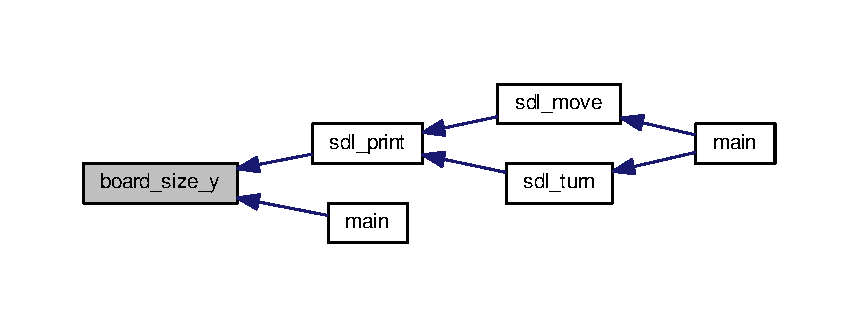
\includegraphics[width=350pt]{snakelib_8h_a01be021996158cf01e830b56e41be904_icgraph}
\end{center}
\end{figure}


\index{snakelib.\+h@{snakelib.\+h}!choc\+\_\+sc@{choc\+\_\+sc}}
\index{choc\+\_\+sc@{choc\+\_\+sc}!snakelib.\+h@{snakelib.\+h}}
\subsubsection[{\texorpdfstring{choc\+\_\+sc(snake const $\ast$s1, snake const $\ast$s2)}{choc_sc(snake const *s1, snake const *s2)}}]{\setlength{\rightskip}{0pt plus 5cm}bool choc\+\_\+sc (
\begin{DoxyParamCaption}
\item[{{\bf snake} const $\ast$}]{s1, }
\item[{{\bf snake} const $\ast$}]{s2}
\end{DoxyParamCaption}
)}\hypertarget{snakelib_8h_ab72d8c937b91594a9c27b30c05a08a75}{}\label{snakelib_8h_ab72d8c937b91594a9c27b30c05a08a75}

\begin{DoxyCode}
490 \{
491     \textcolor{keywordflow}{if} ((*s1)->x == (*s2)->x && (*s1)->y == (*s2)->y)
492         \textcolor{keywordflow}{return} \textcolor{keyword}{true};
493     \textcolor{keywordflow}{return} \textcolor{keyword}{false};
494 \}
\end{DoxyCode}
\index{snakelib.\+h@{snakelib.\+h}!choc\+\_\+snake@{choc\+\_\+snake}}
\index{choc\+\_\+snake@{choc\+\_\+snake}!snakelib.\+h@{snakelib.\+h}}
\subsubsection[{\texorpdfstring{choc\+\_\+snake(snake const $\ast$s1, snake const $\ast$s2)}{choc_snake(snake const *s1, snake const *s2)}}]{\setlength{\rightskip}{0pt plus 5cm}bool choc\+\_\+snake (
\begin{DoxyParamCaption}
\item[{{\bf snake} const $\ast$}]{s1, }
\item[{{\bf snake} const $\ast$}]{s2}
\end{DoxyParamCaption}
)}\hypertarget{snakelib_8h_ab96735ae82693727289ffe22fc940235}{}\label{snakelib_8h_ab96735ae82693727289ffe22fc940235}


test choc entre deux snake 


\begin{DoxyCode}
478 \{
479     \hyperlink{structsnake}{snake} tmp = (*s2)->next;
480     \textcolor{keywordflow}{while}(tmp)
481     \{
482         \textcolor{keywordflow}{if}((*s1)->x == tmp->x && (*s1)->y == tmp->y)
483             \textcolor{keywordflow}{return} \textcolor{keyword}{true};
484         tmp = tmp->next;
485     \}
486     \textcolor{keywordflow}{return} \textcolor{keyword}{false};
487 \}
\end{DoxyCode}


Voici le graphe des appelants de cette fonction \+:\nopagebreak
\begin{figure}[H]
\begin{center}
\leavevmode
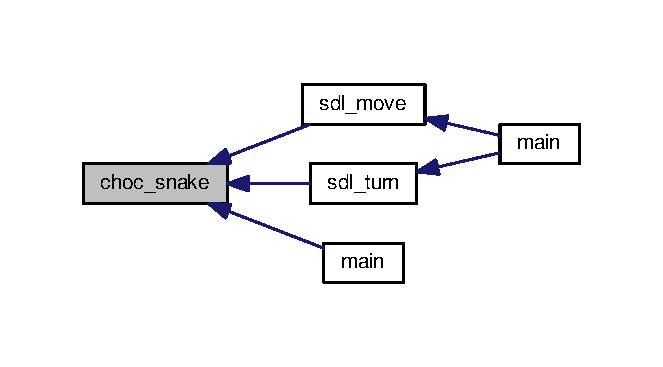
\includegraphics[width=318pt]{snakelib_8h_ab96735ae82693727289ffe22fc940235_icgraph}
\end{center}
\end{figure}


\index{snakelib.\+h@{snakelib.\+h}!choc\+\_\+wall@{choc\+\_\+wall}}
\index{choc\+\_\+wall@{choc\+\_\+wall}!snakelib.\+h@{snakelib.\+h}}
\subsubsection[{\texorpdfstring{choc\+\_\+wall(board const $\ast$b, snake const $\ast$s)}{choc_wall(board const *b, snake const *s)}}]{\setlength{\rightskip}{0pt plus 5cm}bool choc\+\_\+wall (
\begin{DoxyParamCaption}
\item[{{\bf board} const $\ast$}]{b, }
\item[{{\bf snake} const $\ast$}]{s}
\end{DoxyParamCaption}
)}\hypertarget{snakelib_8h_a50fa8a047abfa006a3371a94809e72c4}{}\label{snakelib_8h_a50fa8a047abfa006a3371a94809e72c4}


test choc snake contre le mur 


\begin{DoxyCode}
497 \{
498     \textcolor{keywordflow}{if}((*s)->x == 0) \textcolor{keywordflow}{return} \textcolor{keyword}{true};
499     \textcolor{keywordflow}{if}((*s)->x == \hyperlink{client_8c_a20fdbd342281b7b5b77945c79d176b9f}{b}->\hyperlink{structboard_a45ad83890aed4b92ef175f0eb13cd1f3}{x}-1) \textcolor{keywordflow}{return} \textcolor{keyword}{true};
500     \textcolor{keywordflow}{if}((*s)->y == 0) \textcolor{keywordflow}{return} \textcolor{keyword}{true};
501     \textcolor{keywordflow}{if}((*s)->y == \hyperlink{client_8c_a20fdbd342281b7b5b77945c79d176b9f}{b}->\hyperlink{structboard_a0a1685edc20c5b97527ccd4027d5f8eb}{y}-1) \textcolor{keywordflow}{return} \textcolor{keyword}{true};
502     
503     \textcolor{keywordflow}{return} \textcolor{keyword}{false};
504 \}
\end{DoxyCode}


Voici le graphe des appelants de cette fonction \+:\nopagebreak
\begin{figure}[H]
\begin{center}
\leavevmode
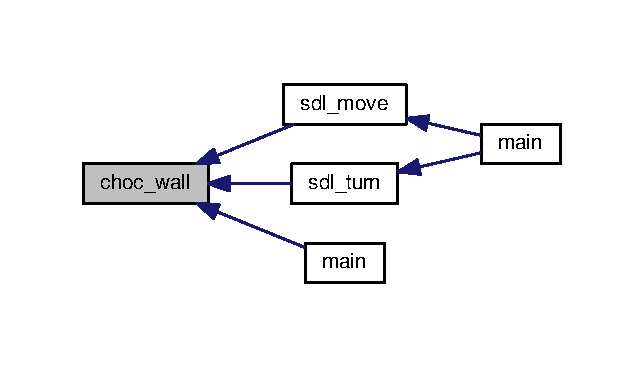
\includegraphics[width=309pt]{snakelib_8h_a50fa8a047abfa006a3371a94809e72c4_icgraph}
\end{center}
\end{figure}


\index{snakelib.\+h@{snakelib.\+h}!move@{move}}
\index{move@{move}!snakelib.\+h@{snakelib.\+h}}
\subsubsection[{\texorpdfstring{move(board $\ast$brdin, snake $\ast$snkin, char id)}{move(board *brdin, snake *snkin, char id)}}]{\setlength{\rightskip}{0pt plus 5cm}void move (
\begin{DoxyParamCaption}
\item[{{\bf board} $\ast$}]{brdin, }
\item[{{\bf snake} $\ast$}]{snkin, }
\item[{char}]{id}
\end{DoxyParamCaption}
)}\hypertarget{snakelib_8h_aa7c9d4fed2b3edb453a4501ba019dc00}{}\label{snakelib_8h_aa7c9d4fed2b3edb453a4501ba019dc00}

\begin{DoxyCode}
371 \{
372     \textcolor{keywordtype}{int} x,y,dx,dy;
373     \hyperlink{snakelib_8c_aa723bfe337f8108975b8d36292b422d1}{snake\_del}(snkin, &x, &y);
374     \hyperlink{snakelib_8c_a12954721537f652c82e9cf23c1bfb0c3}{board\_set}(brdin, x, y, \textcolor{charliteral}{' '});
375     dx = ((*snkin)->x) - ((*snkin)->next->x);
376     dy = ((*snkin)->y) - ((*snkin)->next->y);
377     \hyperlink{snakelib_8c_a17492ac4841b98e25c682f9ff358ea2c}{snake\_add}(snkin, (*snkin)->x+dx , (*snkin)->y+dy);
378     \hyperlink{snakelib_8c_a12954721537f652c82e9cf23c1bfb0c3}{board\_set}(brdin, (*snkin)->\hyperlink{structboard_a45ad83890aed4b92ef175f0eb13cd1f3}{x} ,(*snkin)->y , \textcolor{keywordtype}{id});
379 \}
\end{DoxyCode}


Voici le graphe d\textquotesingle{}appel pour cette fonction \+:\nopagebreak
\begin{figure}[H]
\begin{center}
\leavevmode
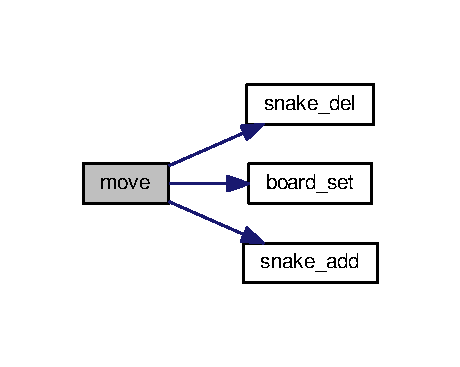
\includegraphics[width=221pt]{snakelib_8h_aa7c9d4fed2b3edb453a4501ba019dc00_cgraph}
\end{center}
\end{figure}




Voici le graphe des appelants de cette fonction \+:\nopagebreak
\begin{figure}[H]
\begin{center}
\leavevmode
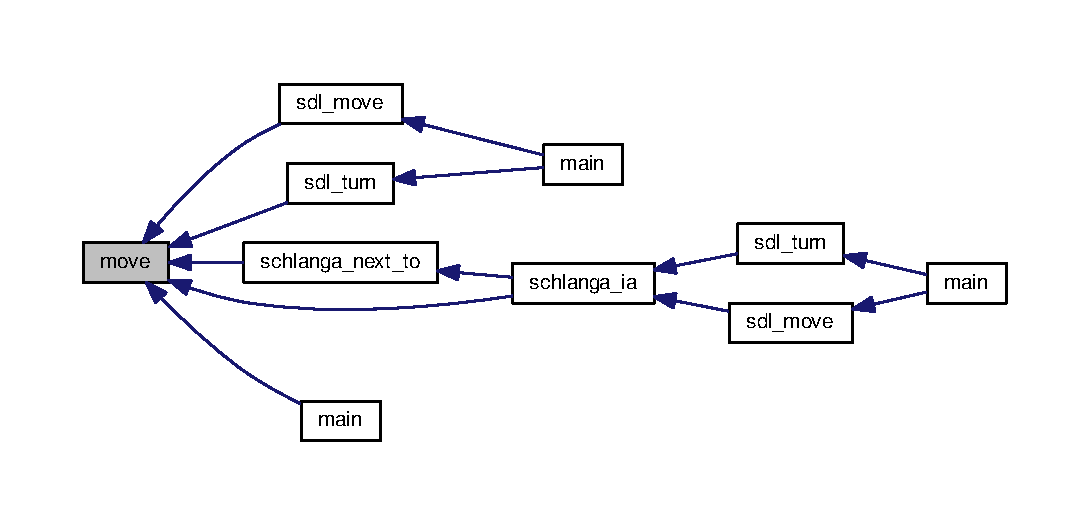
\includegraphics[width=350pt]{snakelib_8h_aa7c9d4fed2b3edb453a4501ba019dc00_icgraph}
\end{center}
\end{figure}


\index{snakelib.\+h@{snakelib.\+h}!snake\+\_\+add@{snake\+\_\+add}}
\index{snake\+\_\+add@{snake\+\_\+add}!snakelib.\+h@{snakelib.\+h}}
\subsubsection[{\texorpdfstring{snake\+\_\+add(snake $\ast$snkin, int x, int y)}{snake_add(snake *snkin, int x, int y)}}]{\setlength{\rightskip}{0pt plus 5cm}void snake\+\_\+add (
\begin{DoxyParamCaption}
\item[{{\bf snake} $\ast$}]{snkin, }
\item[{int}]{x, }
\item[{int}]{y}
\end{DoxyParamCaption}
)}\hypertarget{snakelib_8h_a17492ac4841b98e25c682f9ff358ea2c}{}\label{snakelib_8h_a17492ac4841b98e25c682f9ff358ea2c}


un snake est équivalent à une file d\textquotesingle{}attente (F\+I\+FO « first in, first out »), cette fonction permet d\textquotesingle{}ajouter à l\textquotesingle{}entête de la liste 


\begin{DoxyParams}{Paramètres}
{\em snake} & $\ast$snkin\+: adresse d\textquotesingle{}un snake \\
\hline
{\em int} & x, int y\+: coordonnée du nouvel élément \\
\hline
\end{DoxyParams}
\begin{DoxyReturn}{Renvoie}
fonction de type void 
\end{DoxyReturn}
define list output with coord x,y

the next element is list input

edit list input( $\ast$input=output) 
\begin{DoxyCode}
192 \{
194     \hyperlink{structsnake}{snake} snkout=malloc(\textcolor{keyword}{sizeof}(\hyperlink{struct__snake}{\_snake}));
195     snkout->x = x;
196     snkout->y = y;
198     snkout->next = *snkin;
200     *snkin = snkout;
201 \}
\end{DoxyCode}


Voici le graphe des appelants de cette fonction \+:\nopagebreak
\begin{figure}[H]
\begin{center}
\leavevmode
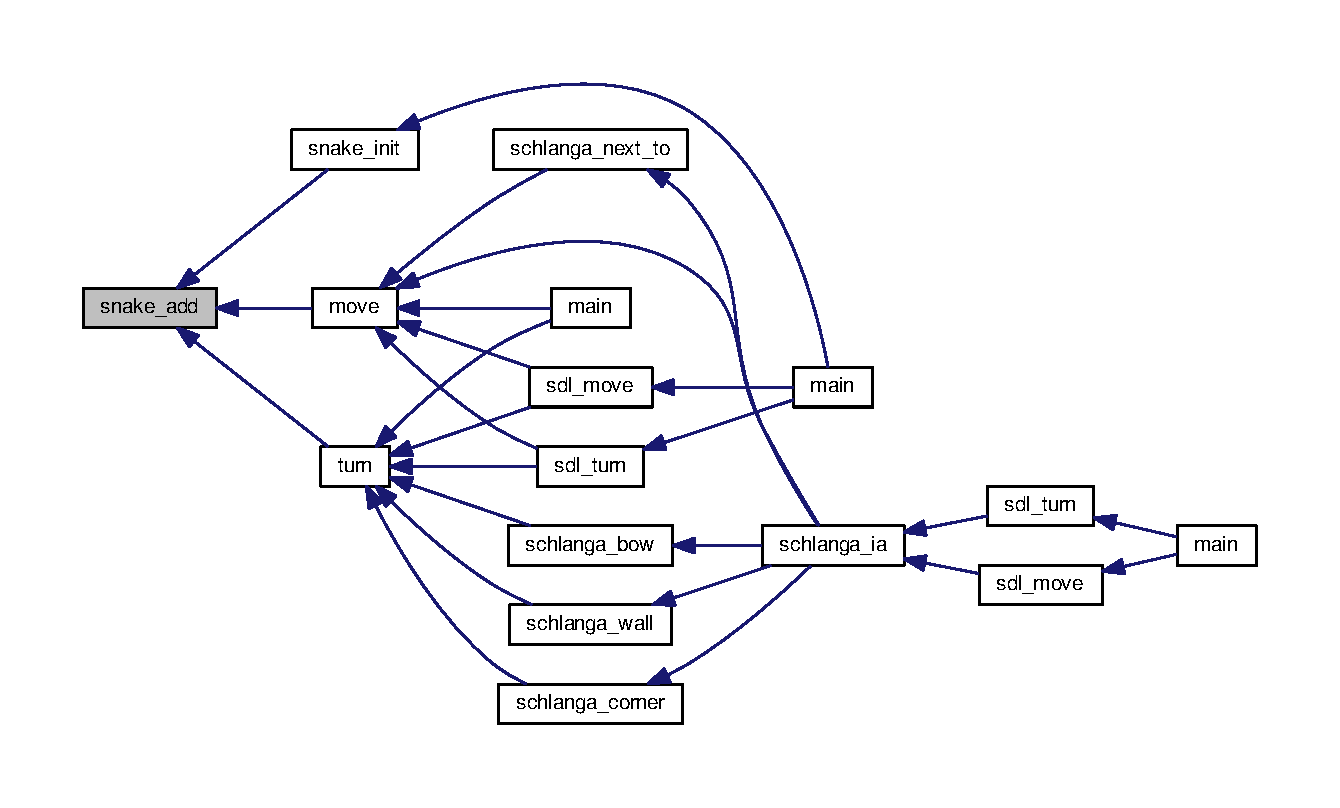
\includegraphics[width=350pt]{snakelib_8h_a17492ac4841b98e25c682f9ff358ea2c_icgraph}
\end{center}
\end{figure}


\index{snakelib.\+h@{snakelib.\+h}!snake\+\_\+addl@{snake\+\_\+addl}}
\index{snake\+\_\+addl@{snake\+\_\+addl}!snakelib.\+h@{snakelib.\+h}}
\subsubsection[{\texorpdfstring{snake\+\_\+addl(snake $\ast$snkin, int x, int y)}{snake_addl(snake *snkin, int x, int y)}}]{\setlength{\rightskip}{0pt plus 5cm}void snake\+\_\+addl (
\begin{DoxyParamCaption}
\item[{{\bf snake} $\ast$}]{snkin, }
\item[{int}]{x, }
\item[{int}]{y}
\end{DoxyParamCaption}
)}\hypertarget{snakelib_8h_a6b2f097d4deefee8b8f8d809691f44ce}{}\label{snakelib_8h_a6b2f097d4deefee8b8f8d809691f44ce}

\begin{DoxyCode}
262 \{
263     \hyperlink{structsnake}{snake} \textcolor{keyword}{new} = malloc(\textcolor{keyword}{sizeof}(\hyperlink{struct__snake}{\_snake}));
264     *\textcolor{keyword}{new} = (\hyperlink{snakelib_8h_a37a403a92b4650960d024935a50e67e9}{\_snake})
265     \{
266         .x = x,
267         .y = y,
268         .next = NULL,
269     \};
270     \hyperlink{structsnake}{snake} tmp = *snkin;
271     \textcolor{keywordflow}{while}(tmp->next != NULL)
272     \{
273         tmp = tmp->next;
274     \}
275     tmp->next = \textcolor{keyword}{new};
276 \}
\end{DoxyCode}


Voici le graphe des appelants de cette fonction \+:\nopagebreak
\begin{figure}[H]
\begin{center}
\leavevmode
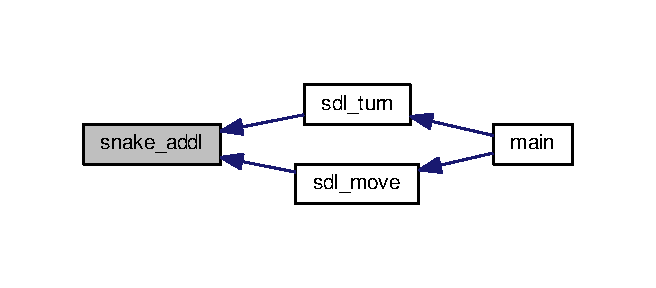
\includegraphics[width=315pt]{snakelib_8h_a6b2f097d4deefee8b8f8d809691f44ce_icgraph}
\end{center}
\end{figure}


\index{snakelib.\+h@{snakelib.\+h}!snake\+\_\+apple@{snake\+\_\+apple}}
\index{snake\+\_\+apple@{snake\+\_\+apple}!snakelib.\+h@{snakelib.\+h}}
\subsubsection[{\texorpdfstring{snake\+\_\+apple(snake const $\ast$s, int $\ast$x, int $\ast$y)}{snake_apple(snake const *s, int *x, int *y)}}]{\setlength{\rightskip}{0pt plus 5cm}bool snake\+\_\+apple (
\begin{DoxyParamCaption}
\item[{{\bf snake} const $\ast$}]{s, }
\item[{int $\ast$}]{x, }
\item[{int $\ast$}]{y}
\end{DoxyParamCaption}
)}\hypertarget{snakelib_8h_a9c77869dc19e2c9bc443ab997aad1f4f}{}\label{snakelib_8h_a9c77869dc19e2c9bc443ab997aad1f4f}

\begin{DoxyCode}
527 \{
528     \textcolor{keywordflow}{if}(\hyperlink{snakelib_8c_a01c30f2556498b7887cc5ff5a88119ca}{snake\_x}(\hyperlink{client_8c_a71e92e96b65208605aca57598cc827f1}{s}) == *x && \hyperlink{snakelib_8c_ad0e10e1a230ae236d8b5fe92e2559378}{snake\_y}(\hyperlink{client_8c_a71e92e96b65208605aca57598cc827f1}{s}) == *y) \textcolor{keywordflow}{return} \textcolor{keyword}{true};
529     \textcolor{keywordflow}{return} \textcolor{keyword}{false};
530 \}
\end{DoxyCode}


Voici le graphe d\textquotesingle{}appel pour cette fonction \+:\nopagebreak
\begin{figure}[H]
\begin{center}
\leavevmode
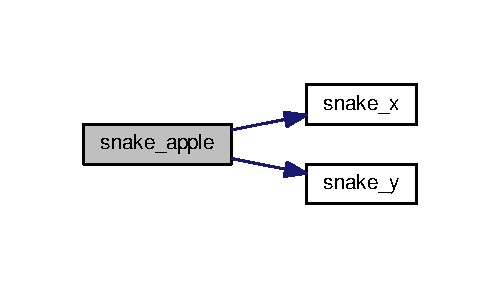
\includegraphics[width=240pt]{snakelib_8h_a9c77869dc19e2c9bc443ab997aad1f4f_cgraph}
\end{center}
\end{figure}




Voici le graphe des appelants de cette fonction \+:\nopagebreak
\begin{figure}[H]
\begin{center}
\leavevmode
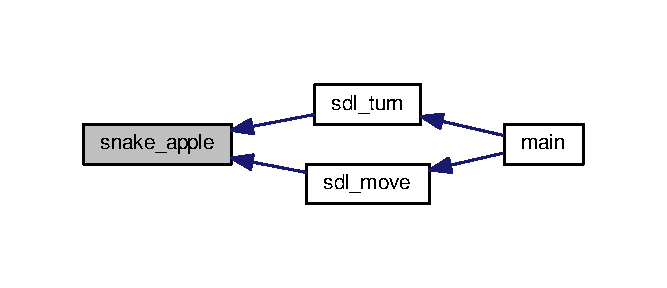
\includegraphics[width=320pt]{snakelib_8h_a9c77869dc19e2c9bc443ab997aad1f4f_icgraph}
\end{center}
\end{figure}


\index{snakelib.\+h@{snakelib.\+h}!snake\+\_\+del@{snake\+\_\+del}}
\index{snake\+\_\+del@{snake\+\_\+del}!snakelib.\+h@{snakelib.\+h}}
\subsubsection[{\texorpdfstring{snake\+\_\+del(snake $\ast$snkin, int $\ast$x, int $\ast$y)}{snake_del(snake *snkin, int *x, int *y)}}]{\setlength{\rightskip}{0pt plus 5cm}void snake\+\_\+del (
\begin{DoxyParamCaption}
\item[{{\bf snake} $\ast$}]{snkin, }
\item[{int $\ast$}]{x, }
\item[{int $\ast$}]{y}
\end{DoxyParamCaption}
)}\hypertarget{snakelib_8h_aa723bfe337f8108975b8d36292b422d1}{}\label{snakelib_8h_aa723bfe337f8108975b8d36292b422d1}


un snake est équivalent à une file d\textquotesingle{}attente (F\+I\+FO « first in, first out »), cette fonction permet de supprimer au queue de la liste 


\begin{DoxyParams}{Paramètres}
{\em snake} & $\ast$snkin\+: adresse d\textquotesingle{}un snake \\
\hline
{\em snake} & int $\ast$x, int $\ast$y\+: adresses de deux entiers pour pouvoir récupérer les coordonnées d\textquotesingle{}élément supprimer \\
\hline
\end{DoxyParams}
\begin{DoxyReturn}{Renvoie}
fonction de type void 
\end{DoxyReturn}
if the list is empty

default value x=-\/1 y=-\/1

if the list contains only one item

we move along the linked list keeping the last two consecutive element
\begin{DoxyCode}
215 \{
216     \textcolor{keywordflow}{if}(*snkin == NULL)
217     \{
219         \textcolor{keywordflow}{if}((x != NULL) && (y != NULL))
220         \{
222             *x = -1;
223             *y = -1;
224         \}
225     \}
226     \textcolor{keywordflow}{else} \textcolor{keywordflow}{if}((*snkin)->next == NULL)
227     \{
228 
230         \textcolor{keywordflow}{if}((x != NULL) && (y != NULL))
231         \{
232             *x = (*snkin)->x;
233             *y = (*snkin)->y;
234         \}
235         free((*snkin));
236         *snkin = NULL;
237     \}
238     \textcolor{keywordflow}{else}
239     \{
244         \hyperlink{structsnake}{snake} tmp1 = *snkin;
245         \hyperlink{structsnake}{snake} tmp2 = *snkin;
246         \textcolor{keywordflow}{while}(tmp1->next != NULL)
247         \{
248             tmp2 = tmp1;
249             tmp1 = tmp1->next;
250         \}
251         \textcolor{keywordflow}{if}((x != NULL) && (y != NULL))
252         \{
253             *x = tmp1->x;
254             *y = tmp1->y;
255         \}
256         tmp2->next = NULL;
257         free(tmp1);
258     \}
259 \}
\end{DoxyCode}


Voici le graphe des appelants de cette fonction \+:\nopagebreak
\begin{figure}[H]
\begin{center}
\leavevmode
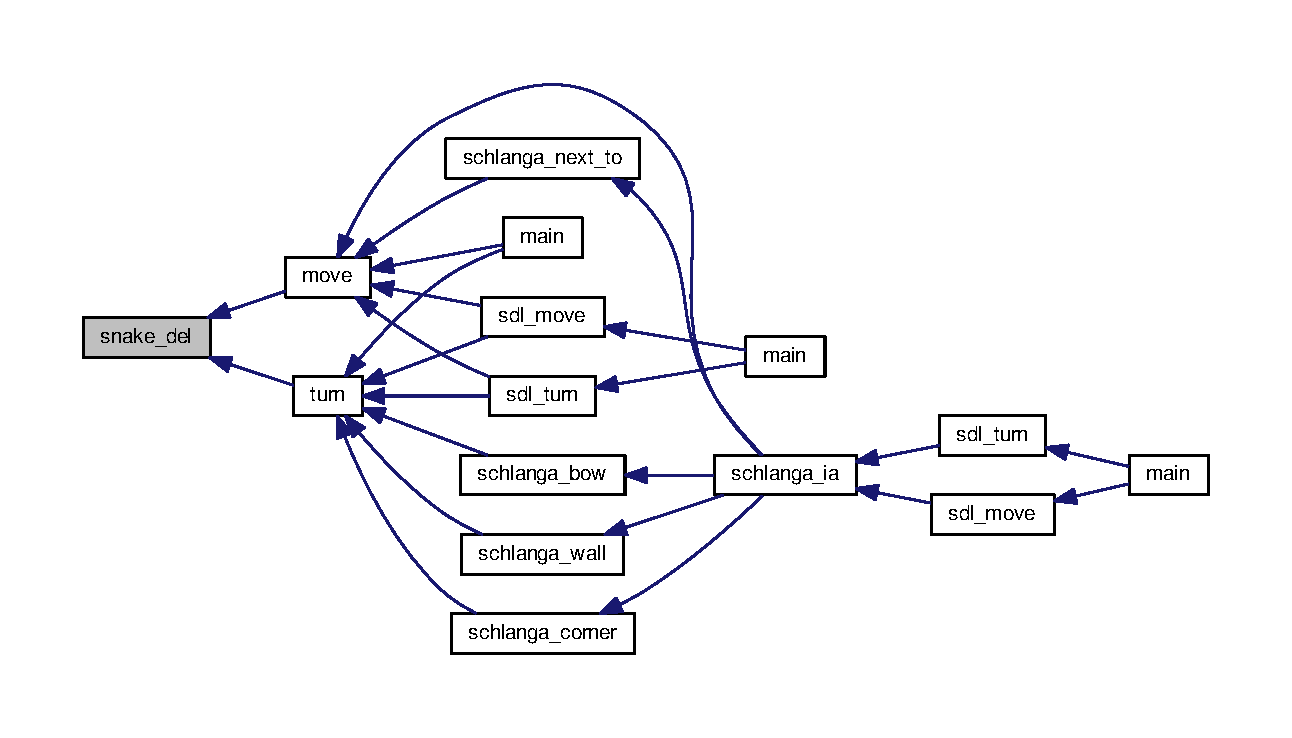
\includegraphics[width=350pt]{snakelib_8h_aa723bfe337f8108975b8d36292b422d1_icgraph}
\end{center}
\end{figure}


\index{snakelib.\+h@{snakelib.\+h}!snake\+\_\+free@{snake\+\_\+free}}
\index{snake\+\_\+free@{snake\+\_\+free}!snakelib.\+h@{snakelib.\+h}}
\subsubsection[{\texorpdfstring{snake\+\_\+free(snake $\ast$snkin)}{snake_free(snake *snkin)}}]{\setlength{\rightskip}{0pt plus 5cm}void snake\+\_\+free (
\begin{DoxyParamCaption}
\item[{{\bf snake} $\ast$}]{snkin}
\end{DoxyParamCaption}
)}\hypertarget{snakelib_8h_ae2b728ff11f9b12d88715ddef95639c9}{}\label{snakelib_8h_ae2b728ff11f9b12d88715ddef95639c9}


libérer la mémoire 


\begin{DoxyParams}{Paramètres}
{\em adresse} & du snake \\
\hline
\end{DoxyParams}
\begin{DoxyReturn}{Renvoie}
fonction de type void 
\end{DoxyReturn}

\begin{DoxyCode}
309 \{
310     \hyperlink{structsnake}{snake} tmp = *snkin;
311     \hyperlink{structsnake}{snake} tmpnext;
312     
313     \textcolor{keywordflow}{while}(tmp != NULL)
314     \{
315         tmpnext = tmp->next;
316         free(tmp);
317         tmp = tmpnext;
318     \}
319     
320     *snkin = NULL;
321 \}
\end{DoxyCode}


Voici le graphe des appelants de cette fonction \+:\nopagebreak
\begin{figure}[H]
\begin{center}
\leavevmode
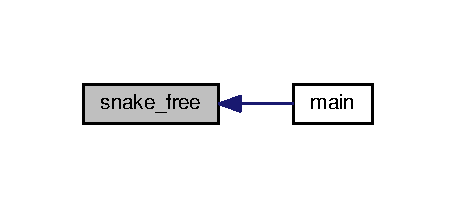
\includegraphics[width=219pt]{snakelib_8h_ae2b728ff11f9b12d88715ddef95639c9_icgraph}
\end{center}
\end{figure}


\index{snakelib.\+h@{snakelib.\+h}!snake\+\_\+getl@{snake\+\_\+getl}}
\index{snake\+\_\+getl@{snake\+\_\+getl}!snakelib.\+h@{snakelib.\+h}}
\subsubsection[{\texorpdfstring{snake\+\_\+getl(snake $\ast$snkin, int $\ast$x, int $\ast$y)}{snake_getl(snake *snkin, int *x, int *y)}}]{\setlength{\rightskip}{0pt plus 5cm}void snake\+\_\+getl (
\begin{DoxyParamCaption}
\item[{{\bf snake} $\ast$}]{snkin, }
\item[{int $\ast$}]{x, }
\item[{int $\ast$}]{y}
\end{DoxyParamCaption}
)}\hypertarget{snakelib_8h_a9f15dca26b0f46aae4e1e5cf30db9ab9}{}\label{snakelib_8h_a9f15dca26b0f46aae4e1e5cf30db9ab9}

\begin{DoxyCode}
279 \{
280     \textcolor{keywordflow}{if}(*snkin == NULL)
281     \{
282         *x = -1;
283         *y = -1;
284     \}
285     \textcolor{keywordflow}{else} \textcolor{keywordflow}{if}((*snkin)->next == NULL)
286     \{
287         *x = (*snkin)->x;
288         *y = (*snkin)->y;
289     \}
290     \textcolor{keywordflow}{else}
291     \{
292         \hyperlink{structsnake}{snake} tmp = *snkin;
293         \textcolor{keywordflow}{while}(tmp->next != NULL)
294         \{
295             tmp = tmp->next;
296         \}
297         *x = tmp->x;
298         *y = tmp->y;
299     \}
300 \}
\end{DoxyCode}


Voici le graphe des appelants de cette fonction \+:\nopagebreak
\begin{figure}[H]
\begin{center}
\leavevmode
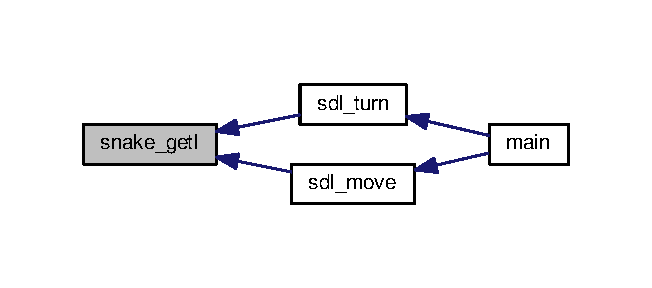
\includegraphics[width=313pt]{snakelib_8h_a9f15dca26b0f46aae4e1e5cf30db9ab9_icgraph}
\end{center}
\end{figure}


\index{snakelib.\+h@{snakelib.\+h}!snake\+\_\+init@{snake\+\_\+init}}
\index{snake\+\_\+init@{snake\+\_\+init}!snakelib.\+h@{snakelib.\+h}}
\subsubsection[{\texorpdfstring{snake\+\_\+init(board $\ast$brdin, snake $\ast$snkin, int len, char id)}{snake_init(board *brdin, snake *snkin, int len, char id)}}]{\setlength{\rightskip}{0pt plus 5cm}void snake\+\_\+init (
\begin{DoxyParamCaption}
\item[{{\bf board} $\ast$}]{brdin, }
\item[{{\bf snake} $\ast$}]{snkin, }
\item[{int}]{len, }
\item[{char}]{id}
\end{DoxyParamCaption}
)}\hypertarget{snakelib_8h_ac696fcc76930ea0badb2f263dd479c93}{}\label{snakelib_8h_ac696fcc76930ea0badb2f263dd479c93}


init a snake 


\begin{DoxyCode}
429 \{
430     \textcolor{keywordflow}{if}(\textcolor{keywordtype}{id} == \textcolor{charliteral}{'@'})
431     \{
432         
433         \hyperlink{snakelib_8c_a17492ac4841b98e25c682f9ff358ea2c}{snake\_add}( snkin, brdin->\hyperlink{structboard_a45ad83890aed4b92ef175f0eb13cd1f3}{x} / 2, brdin->\hyperlink{structboard_a0a1685edc20c5b97527ccd4027d5f8eb}{y} - 2 );
434         \hyperlink{snakelib_8c_a12954721537f652c82e9cf23c1bfb0c3}{board\_set}( brdin, (*snkin)->\hyperlink{structboard_a45ad83890aed4b92ef175f0eb13cd1f3}{x}, (*snkin)->y, \textcolor{keywordtype}{id} );
435         
436         \textcolor{keywordtype}{int} i;
437         \textcolor{keywordflow}{for}(i = 0; i < len - 1; i++)
438         \{
439             \hyperlink{snakelib_8c_a17492ac4841b98e25c682f9ff358ea2c}{snake\_add}( snkin, (*snkin)->x, (*snkin)->y -1 );
440             \hyperlink{snakelib_8c_a12954721537f652c82e9cf23c1bfb0c3}{board\_set}( brdin, (*snkin)->\hyperlink{structboard_a45ad83890aed4b92ef175f0eb13cd1f3}{x}, (*snkin)->y, \textcolor{keywordtype}{id} );
441         \}
442         
443     \}
444     
445     \textcolor{keywordflow}{if}(\textcolor{keywordtype}{id} == \textcolor{charliteral}{'&'})
446     \{
447         
448         \hyperlink{snakelib_8c_a17492ac4841b98e25c682f9ff358ea2c}{snake\_add}( snkin, brdin->\hyperlink{structboard_a45ad83890aed4b92ef175f0eb13cd1f3}{x} / 2, 1 );
449         \hyperlink{snakelib_8c_a12954721537f652c82e9cf23c1bfb0c3}{board\_set}( brdin, (*snkin)->\hyperlink{structboard_a45ad83890aed4b92ef175f0eb13cd1f3}{x}, (*snkin)->y, \textcolor{keywordtype}{id} );
450         
451         \textcolor{keywordtype}{int} i;
452         \textcolor{keywordflow}{for}(i = 0; i < len - 1; i++)
453         \{
454             \hyperlink{snakelib_8c_a17492ac4841b98e25c682f9ff358ea2c}{snake\_add}( snkin, (*snkin)->x, (*snkin)->y +1 );
455             \hyperlink{snakelib_8c_a12954721537f652c82e9cf23c1bfb0c3}{board\_set}( brdin, (*snkin)->\hyperlink{structboard_a45ad83890aed4b92ef175f0eb13cd1f3}{x}, (*snkin)->y, \textcolor{keywordtype}{id} );
456         \}
457         
458     \}
459 
460     \textcolor{keywordflow}{if}(\textcolor{keywordtype}{id} == \textcolor{charliteral}{'+'})
461     \{
462         
463         \hyperlink{snakelib_8c_a17492ac4841b98e25c682f9ff358ea2c}{snake\_add}( snkin, 1, brdin->\hyperlink{structboard_a0a1685edc20c5b97527ccd4027d5f8eb}{y} / 2 );
464         \hyperlink{snakelib_8c_a12954721537f652c82e9cf23c1bfb0c3}{board\_set}( brdin, (*snkin)->\hyperlink{structboard_a45ad83890aed4b92ef175f0eb13cd1f3}{x}, (*snkin)->y, \textcolor{keywordtype}{id} );
465         
466         \textcolor{keywordtype}{int} i;
467         \textcolor{keywordflow}{for}(i = 0; i < len - 1; i++)
468         \{
469             \hyperlink{snakelib_8c_a17492ac4841b98e25c682f9ff358ea2c}{snake\_add}( snkin, (*snkin)->x + 1, (*snkin)->y);
470             \hyperlink{snakelib_8c_a12954721537f652c82e9cf23c1bfb0c3}{board\_set}( brdin, (*snkin)->\hyperlink{structboard_a45ad83890aed4b92ef175f0eb13cd1f3}{x}, (*snkin)->y, 1 );
471         \}
472         
473     \}
474     
475 \}
\end{DoxyCode}


Voici le graphe d\textquotesingle{}appel pour cette fonction \+:\nopagebreak
\begin{figure}[H]
\begin{center}
\leavevmode
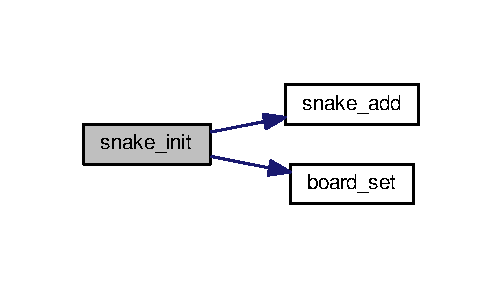
\includegraphics[width=241pt]{snakelib_8h_ac696fcc76930ea0badb2f263dd479c93_cgraph}
\end{center}
\end{figure}




Voici le graphe des appelants de cette fonction \+:\nopagebreak
\begin{figure}[H]
\begin{center}
\leavevmode
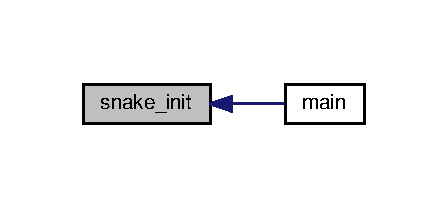
\includegraphics[width=215pt]{snakelib_8h_ac696fcc76930ea0badb2f263dd479c93_icgraph}
\end{center}
\end{figure}


\index{snakelib.\+h@{snakelib.\+h}!snake\+\_\+print@{snake\+\_\+print}}
\index{snake\+\_\+print@{snake\+\_\+print}!snakelib.\+h@{snakelib.\+h}}
\subsubsection[{\texorpdfstring{snake\+\_\+print(const snake $\ast$snkin)}{snake_print(const snake *snkin)}}]{\setlength{\rightskip}{0pt plus 5cm}void snake\+\_\+print (
\begin{DoxyParamCaption}
\item[{const {\bf snake} $\ast$}]{snkin}
\end{DoxyParamCaption}
)}\hypertarget{snakelib_8h_a08f653b84e023db977cc57ff5fc8debf}{}\label{snakelib_8h_a08f653b84e023db977cc57ff5fc8debf}

\begin{DoxyCode}
332 \{
333     \hyperlink{structsnake}{snake} tmp = *snkin;
334     \textcolor{keywordflow}{while}(tmp != NULL)
335     \{
336         printf(\textcolor{stringliteral}{"[%d:%d]"}, tmp->x, tmp->y);
337         tmp = tmp->next;
338     \}
339     printf(\textcolor{stringliteral}{"\(\backslash\)n"});
340 \}
\end{DoxyCode}


Voici le graphe des appelants de cette fonction \+:\nopagebreak
\begin{figure}[H]
\begin{center}
\leavevmode
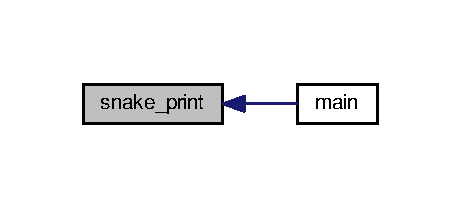
\includegraphics[width=221pt]{snakelib_8h_a08f653b84e023db977cc57ff5fc8debf_icgraph}
\end{center}
\end{figure}


\index{snakelib.\+h@{snakelib.\+h}!turn@{turn}}
\index{turn@{turn}!snakelib.\+h@{snakelib.\+h}}
\subsubsection[{\texorpdfstring{turn(board $\ast$brdin, snake $\ast$snkin, int drctn, char id)}{turn(board *brdin, snake *snkin, int drctn, char id)}}]{\setlength{\rightskip}{0pt plus 5cm}void turn (
\begin{DoxyParamCaption}
\item[{{\bf board} $\ast$}]{brdin, }
\item[{{\bf snake} $\ast$}]{snkin, }
\item[{int}]{drctn, }
\item[{char}]{id}
\end{DoxyParamCaption}
)}\hypertarget{snakelib_8h_afa428ecb4385e08a82520bec11bafe36}{}\label{snakelib_8h_afa428ecb4385e08a82520bec11bafe36}

\begin{DoxyCode}
394 \{
395     \textcolor{keywordtype}{int} x,y,dx,dy;
396     
397     \hyperlink{snakelib_8c_aa723bfe337f8108975b8d36292b422d1}{snake\_del}(snkin,&x,&y);
398     \hyperlink{snakelib_8c_a12954721537f652c82e9cf23c1bfb0c3}{board\_set}(brdin,x,y, \textcolor{charliteral}{' '});
399     
400     dx=((*snkin)->x) - ((*snkin)->next->x);
401     dy=((*snkin)->y) - ((*snkin)->next->y);
402     
403     \textcolor{keywordflow}{if}(dx == 1)
404     \{
405         \hyperlink{snakelib_8c_a17492ac4841b98e25c682f9ff358ea2c}{snake\_add}(snkin, (*snkin)->x, (*snkin)->y + drctn);
406         \hyperlink{snakelib_8c_a12954721537f652c82e9cf23c1bfb0c3}{board\_set}(brdin, (*snkin)->\hyperlink{structboard_a45ad83890aed4b92ef175f0eb13cd1f3}{x}, (*snkin)->y, \textcolor{keywordtype}{id});
407     \}
408     
409     \textcolor{keywordflow}{else} \textcolor{keywordflow}{if}(dx == -1)
410     \{
411         \hyperlink{snakelib_8c_a17492ac4841b98e25c682f9ff358ea2c}{snake\_add}(snkin, (*snkin)->x, (*snkin)->y - drctn);
412         \hyperlink{snakelib_8c_a12954721537f652c82e9cf23c1bfb0c3}{board\_set}(brdin, (*snkin)->\hyperlink{structboard_a45ad83890aed4b92ef175f0eb13cd1f3}{x}, (*snkin)->y, \textcolor{keywordtype}{id});
413     \}
414     
415     \textcolor{keywordflow}{else} \textcolor{keywordflow}{if}(dy == 1)
416     \{
417         \hyperlink{snakelib_8c_a17492ac4841b98e25c682f9ff358ea2c}{snake\_add}(snkin,(*snkin)->x-drctn,(*snkin)->y);
418         \hyperlink{snakelib_8c_a12954721537f652c82e9cf23c1bfb0c3}{board\_set}(brdin,(*snkin)->\hyperlink{structboard_a45ad83890aed4b92ef175f0eb13cd1f3}{x},(*snkin)->y,\textcolor{keywordtype}{id});
419     \}
420     
421     \textcolor{keywordflow}{else} \textcolor{keywordflow}{if}(dy == -1)
422     \{
423         \hyperlink{snakelib_8c_a17492ac4841b98e25c682f9ff358ea2c}{snake\_add}(snkin,(*snkin)->x+drctn,(*snkin)->y);
424         \hyperlink{snakelib_8c_a12954721537f652c82e9cf23c1bfb0c3}{board\_set}(brdin,(*snkin)->\hyperlink{structboard_a45ad83890aed4b92ef175f0eb13cd1f3}{x},(*snkin)->y,\textcolor{keywordtype}{id});
425     \}
426 \}
\end{DoxyCode}


Voici le graphe d\textquotesingle{}appel pour cette fonction \+:\nopagebreak
\begin{figure}[H]
\begin{center}
\leavevmode
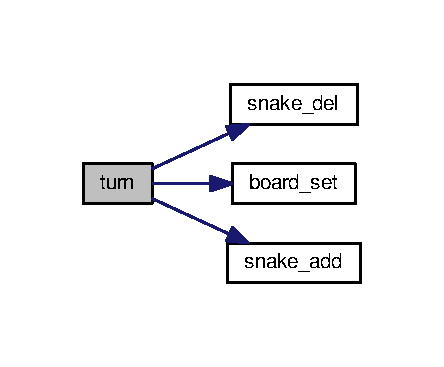
\includegraphics[width=213pt]{snakelib_8h_afa428ecb4385e08a82520bec11bafe36_cgraph}
\end{center}
\end{figure}




Voici le graphe des appelants de cette fonction \+:\nopagebreak
\begin{figure}[H]
\begin{center}
\leavevmode
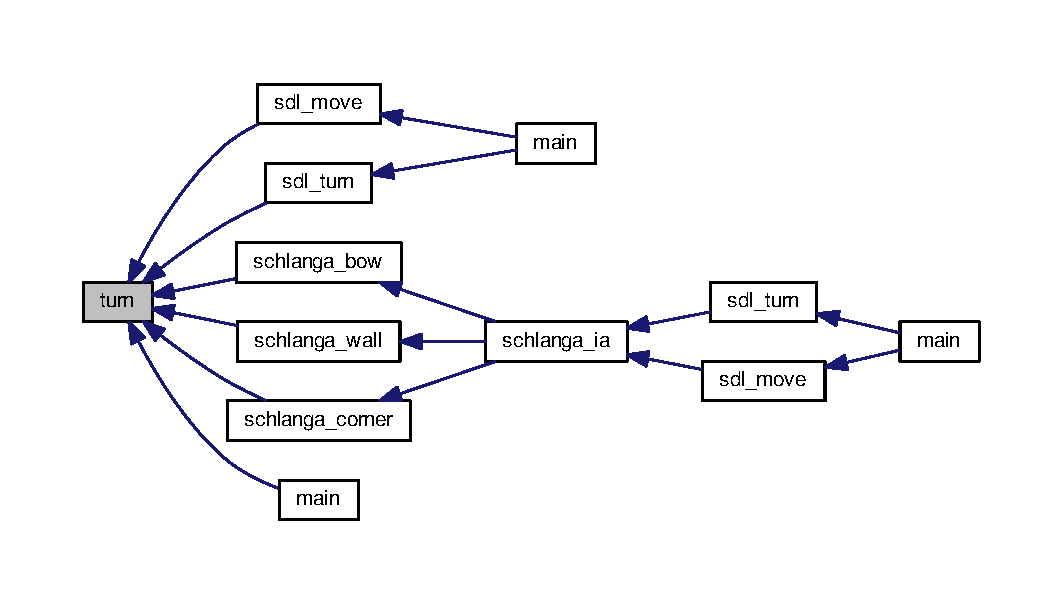
\includegraphics[width=350pt]{snakelib_8h_afa428ecb4385e08a82520bec11bafe36_icgraph}
\end{center}
\end{figure}



\hypertarget{client_8c}{}\section{Référence du fichier S\+O\+U\+R\+C\+E/client.c}
\label{client_8c}\index{S\+O\+U\+R\+C\+E/client.\+c@{S\+O\+U\+R\+C\+E/client.\+c}}
{\ttfamily \#include $<$sys/types.\+h$>$}\\*
{\ttfamily \#include $<$sys/socket.\+h$>$}\\*
{\ttfamily \#include $<$netinet/in.\+h$>$}\\*
{\ttfamily \#include $<$netdb.\+h$>$}\\*
{\ttfamily \#include $<$unistd.\+h$>$}\\*
{\ttfamily \#include $<$pthread.\+h$>$}\\*
{\ttfamily \#include $<$stdbool.\+h$>$}\\*
{\ttfamily \#include $<$stdio.\+h$>$}\\*
{\ttfamily \#include $<$stdlib.\+h$>$}\\*
{\ttfamily \#include $<$strings.\+h$>$}\\*
{\ttfamily \#include \char`\"{}../\+I\+N\+C\+L\+U\+D\+E/snakelib.\+h\char`\"{}}\\*
{\ttfamily \#include $<$S\+D\+L/\+S\+D\+L.\+h$>$}\\*
Graphe des dépendances par inclusion de client.\+c\+:\nopagebreak
\begin{figure}[H]
\begin{center}
\leavevmode
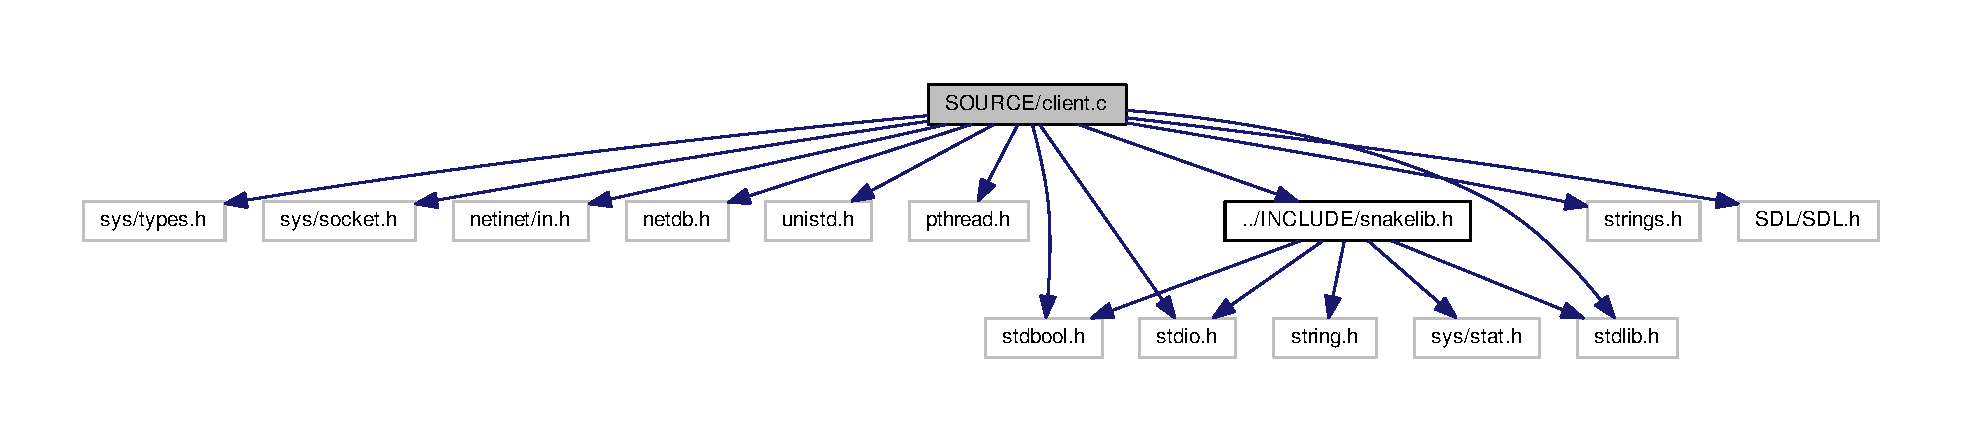
\includegraphics[width=350pt]{client_8c__incl}
\end{center}
\end{figure}
\subsection*{Macros}
\begin{DoxyCompactItemize}
\item 
\#define \hyperlink{client_8c_a18bd5b46e04e0010b0163f03741a2521}{err}(msg)~\{fprintf(stderr, \char`\"{}\%s\textbackslash{}n\char`\"{}, msg);exit(1);\}
\item 
\#define \hyperlink{client_8c_a614217d263be1fb1a5f76e2ff7be19a2}{P\+O\+RT}~1234
\item 
\#define \hyperlink{client_8c_ac9f31f726d2933782e2efda7136a25fd}{A\+D\+DR}~\char`\"{}localhost\char`\"{}
\item 
\#define \hyperlink{client_8c_a9e9d90aaed8d1c89d7431024da9feb39}{tabX}~51
\item 
\#define \hyperlink{client_8c_a8c281530fd59455d29f70006bc720f6d}{tabY}~31
\item 
\#define \hyperlink{client_8c_a8373df012cb4cb326153306f7ebf43f8}{slen}~3
\end{DoxyCompactItemize}
\subsection*{Fonctions}
\begin{DoxyCompactItemize}
\item 
static int \hyperlink{client_8c_a7b1f2521e5756d5157688c8517538a14}{client\+\_\+socket} ()
\item 
void \hyperlink{client_8c_a2cfeae643e415db24e85db6c4994b071}{sdl\+\_\+print} ()
\item 
void $\ast$ \hyperlink{client_8c_af424c7fd4c84203cddfb7230bbe15401}{sdl\+\_\+move} ()
\item 
void $\ast$ \hyperlink{client_8c_ace514d3ea0e685be64430b930ef23b46}{sdl\+\_\+turn} ()
\item 
int \hyperlink{client_8c_ae66f6b31b5ad750f1fe042a706a4e3d4}{main} ()
\end{DoxyCompactItemize}
\subsection*{Variables}
\begin{DoxyCompactItemize}
\item 
pthread\+\_\+t \hyperlink{client_8c_acdb501237bbfd1adad2d00fc7052a767}{threadpt}
\item 
pthread\+\_\+mutex\+\_\+t \hyperlink{client_8c_a4acff8232e4aec9cd5c6dc200ac55ef3}{mutex} = P\+T\+H\+R\+E\+A\+D\+\_\+\+M\+U\+T\+E\+X\+\_\+\+I\+N\+I\+T\+I\+A\+L\+I\+Z\+ER
\item 
S\+D\+L\+\_\+\+Surface $\ast$ \hyperlink{client_8c_ae8dfea36e66ed4b47c61a7ea5212e164}{E}
\item 
S\+D\+L\+\_\+\+Surface $\ast$ \hyperlink{client_8c_a79a54bef7bf02b18264c38fc90549a04}{A}
\item 
S\+D\+L\+\_\+\+Surface $\ast$ \hyperlink{client_8c_ac54b5255531a4799123d0f8dca96a7cc}{B}
\item 
S\+D\+L\+\_\+\+Surface $\ast$ \hyperlink{client_8c_ab7d76262118cf1d4da44315136e542ca}{C}
\item 
S\+D\+L\+\_\+\+Surface $\ast$ \hyperlink{client_8c_aae9bd8b56defc5a6ec9c20b503b59a3a}{D}
\item 
\hyperlink{structboard}{board} \hyperlink{client_8c_a20fdbd342281b7b5b77945c79d176b9f}{b}
\item 
\hyperlink{structsnake}{snake} \hyperlink{client_8c_a71e92e96b65208605aca57598cc827f1}{s}
\item 
\hyperlink{structsnake}{snake} \hyperlink{client_8c_aa6fd7c53c9b79f5a6ccb6f73b383263c}{c}
\item 
bool \hyperlink{client_8c_aab1bde286e010d81472b269b419806d6}{X}
\item 
char \hyperlink{client_8c_af6f0bd3dc13317f895c91323c25c2b8f}{t}
\item 
char \hyperlink{client_8c_a0318530b7ab3cba31a8e7213e34351cc}{o}
\item 
char \hyperlink{client_8c_a6edfa8f60e57212495b55b6b96c92cc5}{r}
\item 
char \hyperlink{client_8c_a70893b9fd599f8c9ed3ed00c52eba44a}{l}
\item 
char \hyperlink{client_8c_a67668278838ab1eb0065ef9218c8de00}{m}
\item 
int \hyperlink{client_8c_a76f11d9a0a47b94f72c2d0e77fb32240}{n}
\end{DoxyCompactItemize}


\subsection{Documentation des macros}
\index{client.\+c@{client.\+c}!A\+D\+DR@{A\+D\+DR}}
\index{A\+D\+DR@{A\+D\+DR}!client.\+c@{client.\+c}}
\subsubsection[{\texorpdfstring{A\+D\+DR}{ADDR}}]{\setlength{\rightskip}{0pt plus 5cm}\#define A\+D\+DR~\char`\"{}localhost\char`\"{}}\hypertarget{client_8c_ac9f31f726d2933782e2efda7136a25fd}{}\label{client_8c_ac9f31f726d2933782e2efda7136a25fd}
\index{client.\+c@{client.\+c}!err@{err}}
\index{err@{err}!client.\+c@{client.\+c}}
\subsubsection[{\texorpdfstring{err}{err}}]{\setlength{\rightskip}{0pt plus 5cm}\#define err(
\begin{DoxyParamCaption}
\item[{}]{msg}
\end{DoxyParamCaption}
)~\{fprintf(stderr, \char`\"{}\%s\textbackslash{}n\char`\"{}, msg);exit(1);\}}\hypertarget{client_8c_a18bd5b46e04e0010b0163f03741a2521}{}\label{client_8c_a18bd5b46e04e0010b0163f03741a2521}
\index{client.\+c@{client.\+c}!P\+O\+RT@{P\+O\+RT}}
\index{P\+O\+RT@{P\+O\+RT}!client.\+c@{client.\+c}}
\subsubsection[{\texorpdfstring{P\+O\+RT}{PORT}}]{\setlength{\rightskip}{0pt plus 5cm}\#define P\+O\+RT~1234}\hypertarget{client_8c_a614217d263be1fb1a5f76e2ff7be19a2}{}\label{client_8c_a614217d263be1fb1a5f76e2ff7be19a2}
\index{client.\+c@{client.\+c}!slen@{slen}}
\index{slen@{slen}!client.\+c@{client.\+c}}
\subsubsection[{\texorpdfstring{slen}{slen}}]{\setlength{\rightskip}{0pt plus 5cm}\#define slen~3}\hypertarget{client_8c_a8373df012cb4cb326153306f7ebf43f8}{}\label{client_8c_a8373df012cb4cb326153306f7ebf43f8}
\index{client.\+c@{client.\+c}!tabX@{tabX}}
\index{tabX@{tabX}!client.\+c@{client.\+c}}
\subsubsection[{\texorpdfstring{tabX}{tabX}}]{\setlength{\rightskip}{0pt plus 5cm}\#define tabX~51}\hypertarget{client_8c_a9e9d90aaed8d1c89d7431024da9feb39}{}\label{client_8c_a9e9d90aaed8d1c89d7431024da9feb39}
\index{client.\+c@{client.\+c}!tabY@{tabY}}
\index{tabY@{tabY}!client.\+c@{client.\+c}}
\subsubsection[{\texorpdfstring{tabY}{tabY}}]{\setlength{\rightskip}{0pt plus 5cm}\#define tabY~31}\hypertarget{client_8c_a8c281530fd59455d29f70006bc720f6d}{}\label{client_8c_a8c281530fd59455d29f70006bc720f6d}


\subsection{Documentation des fonctions}
\index{client.\+c@{client.\+c}!client\+\_\+socket@{client\+\_\+socket}}
\index{client\+\_\+socket@{client\+\_\+socket}!client.\+c@{client.\+c}}
\subsubsection[{\texorpdfstring{client\+\_\+socket()}{client_socket()}}]{\setlength{\rightskip}{0pt plus 5cm}static int client\+\_\+socket (
\begin{DoxyParamCaption}
{}
\end{DoxyParamCaption}
)\hspace{0.3cm}{\ttfamily [static]}}\hypertarget{client_8c_a7b1f2521e5756d5157688c8517538a14}{}\label{client_8c_a7b1f2521e5756d5157688c8517538a14}

\begin{DoxyCode}
38 \{
39     \textcolor{keywordtype}{int} \hyperlink{client_8c_a76f11d9a0a47b94f72c2d0e77fb32240}{n} = socket(AF\_INET, SOCK\_STREAM, 0);
40     \textcolor{keywordflow}{if}(0 > n) \hyperlink{client_8c_a18bd5b46e04e0010b0163f03741a2521}{err}(\textcolor{stringliteral}{"socket()"});
41 
42     \textcolor{keyword}{struct }hostent* server\_host = gethostbyname(\hyperlink{client_8c_ac9f31f726d2933782e2efda7136a25fd}{ADDR});
43     \textcolor{keywordflow}{if}(NULL == server\_host) \hyperlink{client_8c_a18bd5b46e04e0010b0163f03741a2521}{err}(\textcolor{stringliteral}{"gethostbyname()"});
44 
45     \textcolor{keyword}{struct }sockaddr\_in server\_addr;
46     bzero(&server\_addr,\textcolor{keyword}{sizeof}(server\_addr));
47     server\_addr.sin\_family = AF\_INET;
48     server\_addr.sin\_port = htons(\hyperlink{client_8c_a614217d263be1fb1a5f76e2ff7be19a2}{PORT});
49 
50     bcopy((\textcolor{keywordtype}{char} *)server\_host->h\_addr\_list[0], (\textcolor{keywordtype}{char} *)&server\_addr.sin\_addr.s\_addr, server\_host->h\_length)
      ;
51     \textcolor{keywordflow}{if}(0 > connect(n, (\textcolor{keyword}{struct} sockaddr*)&server\_addr, \textcolor{keyword}{sizeof}(server\_addr))) \hyperlink{client_8c_a18bd5b46e04e0010b0163f03741a2521}{err}(\textcolor{stringliteral}{"connect()"});
52     \textcolor{keywordflow}{return} \hyperlink{client_8c_a76f11d9a0a47b94f72c2d0e77fb32240}{n};
53 \}
\end{DoxyCode}


Voici le graphe des appelants de cette fonction \+:\nopagebreak
\begin{figure}[H]
\begin{center}
\leavevmode
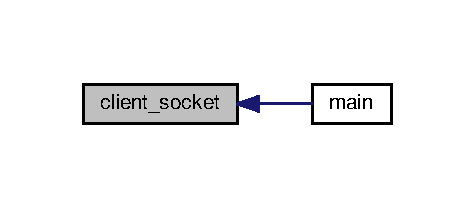
\includegraphics[width=228pt]{client_8c_a7b1f2521e5756d5157688c8517538a14_icgraph}
\end{center}
\end{figure}


\index{client.\+c@{client.\+c}!main@{main}}
\index{main@{main}!client.\+c@{client.\+c}}
\subsubsection[{\texorpdfstring{main()}{main()}}]{\setlength{\rightskip}{0pt plus 5cm}int main (
\begin{DoxyParamCaption}
{}
\end{DoxyParamCaption}
)}\hypertarget{client_8c_ae66f6b31b5ad750f1fe042a706a4e3d4}{}\label{client_8c_ae66f6b31b5ad750f1fe042a706a4e3d4}

\begin{DoxyCode}
204 \{
205     \hyperlink{client_8c_a76f11d9a0a47b94f72c2d0e77fb32240}{n} = \hyperlink{client_8c_a7b1f2521e5756d5157688c8517538a14}{client\_socket}();
206     read(\hyperlink{client_8c_a76f11d9a0a47b94f72c2d0e77fb32240}{n},&\hyperlink{client_8c_af6f0bd3dc13317f895c91323c25c2b8f}{t},\textcolor{keyword}{sizeof}(\textcolor{keywordtype}{char}*));
207     \hyperlink{client_8c_a0318530b7ab3cba31a8e7213e34351cc}{o} = (\hyperlink{client_8c_af6f0bd3dc13317f895c91323c25c2b8f}{t} == \textcolor{charliteral}{'@'})? \textcolor{charliteral}{'&'} : \textcolor{charliteral}{'@'};
208     \hyperlink{client_8c_a67668278838ab1eb0065ef9218c8de00}{m} = \textcolor{charliteral}{'m'};
209     \hyperlink{client_8c_a6edfa8f60e57212495b55b6b96c92cc5}{r} = \textcolor{charliteral}{'r'};
210     \hyperlink{client_8c_a70893b9fd599f8c9ed3ed00c52eba44a}{l} = \textcolor{charliteral}{'l'};
211     \textcolor{comment}{/* la variable globale du jeu */}
212     \hyperlink{client_8c_aab1bde286e010d81472b269b419806d6}{X} = \textcolor{keyword}{true};
213     \textcolor{comment}{/* rand init */}
214     srand(time(0));
215     \textcolor{comment}{/* init board + snake */}
216     \hyperlink{client_8c_a20fdbd342281b7b5b77945c79d176b9f}{b} = \hyperlink{snakelib_8c_a9625331c000178d2cf90ef40d2a8fbf7}{board\_init}(\hyperlink{client_8c_a9e9d90aaed8d1c89d7431024da9feb39}{tabX},\hyperlink{client_8c_a8c281530fd59455d29f70006bc720f6d}{tabY});
217     \hyperlink{snakelib_8c_ac696fcc76930ea0badb2f263dd479c93}{snake\_init}(&\hyperlink{client_8c_a20fdbd342281b7b5b77945c79d176b9f}{b},&\hyperlink{client_8c_a71e92e96b65208605aca57598cc827f1}{s},\hyperlink{client_8c_a8373df012cb4cb326153306f7ebf43f8}{slen},\hyperlink{client_8c_af6f0bd3dc13317f895c91323c25c2b8f}{t});
218     \hyperlink{snakelib_8c_ac696fcc76930ea0badb2f263dd479c93}{snake\_init}(&\hyperlink{client_8c_a20fdbd342281b7b5b77945c79d176b9f}{b},&\hyperlink{client_8c_aa6fd7c53c9b79f5a6ccb6f73b383263c}{c},\hyperlink{client_8c_a8373df012cb4cb326153306f7ebf43f8}{slen},\hyperlink{client_8c_a0318530b7ab3cba31a8e7213e34351cc}{o});
219     \textcolor{comment}{/* init sdl en mode video */}
220     SDL\_Init(SDL\_INIT\_VIDEO);
221     \textcolor{comment}{/* init surface E avec une taille 20*tabX et 20*tabY */}
222     \hyperlink{client_8c_ae8dfea36e66ed4b47c61a7ea5212e164}{E} = SDL\_SetVideoMode(20*\hyperlink{client_8c_a9e9d90aaed8d1c89d7431024da9feb39}{tabX}, 20*\hyperlink{client_8c_a8c281530fd59455d29f70006bc720f6d}{tabY}, 32, SDL\_HWSURFACE);
223     \textcolor{comment}{/* creer le reste des surfaces avec une taille de 20*20 px */}
224     \hyperlink{client_8c_a79a54bef7bf02b18264c38fc90549a04}{A} = SDL\_CreateRGBSurface(SDL\_HWSURFACE, 20, 20, 32, 0, 0, 0, 0);
225     \hyperlink{client_8c_ac54b5255531a4799123d0f8dca96a7cc}{B} = SDL\_CreateRGBSurface(SDL\_HWSURFACE, 20, 20, 32, 0, 0, 0, 0);
226     \hyperlink{client_8c_ab7d76262118cf1d4da44315136e542ca}{C} = SDL\_CreateRGBSurface(SDL\_HWSURFACE, 20, 20, 32, 0, 0, 0, 0);
227     \hyperlink{client_8c_aae9bd8b56defc5a6ec9c20b503b59a3a}{D} = SDL\_CreateRGBSurface(SDL\_HWSURFACE, 20, 20, 32, 0, 0, 0, 0);
228     \textcolor{comment}{/* init avec couleur rgb */}
229     SDL\_FillRect(\hyperlink{client_8c_a79a54bef7bf02b18264c38fc90549a04}{A}, 0, SDL\_MapRGB(\hyperlink{client_8c_ae8dfea36e66ed4b47c61a7ea5212e164}{E}->format, 95, 0, 0));
230     SDL\_FillRect(\hyperlink{client_8c_ac54b5255531a4799123d0f8dca96a7cc}{B}, 0, SDL\_MapRGB(\hyperlink{client_8c_ae8dfea36e66ed4b47c61a7ea5212e164}{E}->format, 137, 137, 137));
231     SDL\_FillRect(\hyperlink{client_8c_ab7d76262118cf1d4da44315136e542ca}{C}, 0, SDL\_MapRGB(\hyperlink{client_8c_ae8dfea36e66ed4b47c61a7ea5212e164}{E}->format, 47, 47, 47));
232     SDL\_FillRect(\hyperlink{client_8c_aae9bd8b56defc5a6ec9c20b503b59a3a}{D}, 0, SDL\_MapRGB(\hyperlink{client_8c_ae8dfea36e66ed4b47c61a7ea5212e164}{E}->format, 157, 62, 12));
233     \textcolor{comment}{/* init barre de fenetre */}
234     SDL\_WM\_SetCaption(\textcolor{stringliteral}{"Snack"}, 0);
235     \textcolor{comment}{/* nos variabe de thread */}
236     pthread\_t thread\_turn;
237     pthread\_t thread\_move;
238     \textcolor{comment}{/* creer les thread */}
239     pthread\_create (&thread\_turn, 0, &\hyperlink{client_8c_ace514d3ea0e685be64430b930ef23b46}{sdl\_turn}, 0);
240     pthread\_create (&thread\_move, 0, &\hyperlink{client_8c_af424c7fd4c84203cddfb7230bbe15401}{sdl\_move},0);
241     \textcolor{comment}{/* attendre leurs fin */}
242     pthread\_join(thread\_turn, 0);
243     pthread\_join(thread\_move, 0);
244     \textcolor{comment}{/* libere surface */}
245     SDL\_FreeSurface(\hyperlink{client_8c_ae8dfea36e66ed4b47c61a7ea5212e164}{E});
246     SDL\_FreeSurface(\hyperlink{client_8c_a79a54bef7bf02b18264c38fc90549a04}{A});
247     SDL\_FreeSurface(\hyperlink{client_8c_ac54b5255531a4799123d0f8dca96a7cc}{B});
248     SDL\_FreeSurface(\hyperlink{client_8c_ab7d76262118cf1d4da44315136e542ca}{C});
249     \textcolor{comment}{/* libere board + snake */}
250     \hyperlink{snakelib_8c_a223ea5e585467eee652b6b3b7a59e0c9}{board\_free}(&\hyperlink{client_8c_a20fdbd342281b7b5b77945c79d176b9f}{b});
251     \hyperlink{snakelib_8c_ae2b728ff11f9b12d88715ddef95639c9}{snake\_free}(&\hyperlink{client_8c_a71e92e96b65208605aca57598cc827f1}{s});
252     \hyperlink{snakelib_8c_ae2b728ff11f9b12d88715ddef95639c9}{snake\_free}(&\hyperlink{client_8c_aa6fd7c53c9b79f5a6ccb6f73b383263c}{c});
253     SDL\_Quit();
254     \textcolor{keywordflow}{return} 0;
255 \}\end{DoxyCode}


Voici le graphe d\textquotesingle{}appel pour cette fonction \+:\nopagebreak
\begin{figure}[H]
\begin{center}
\leavevmode
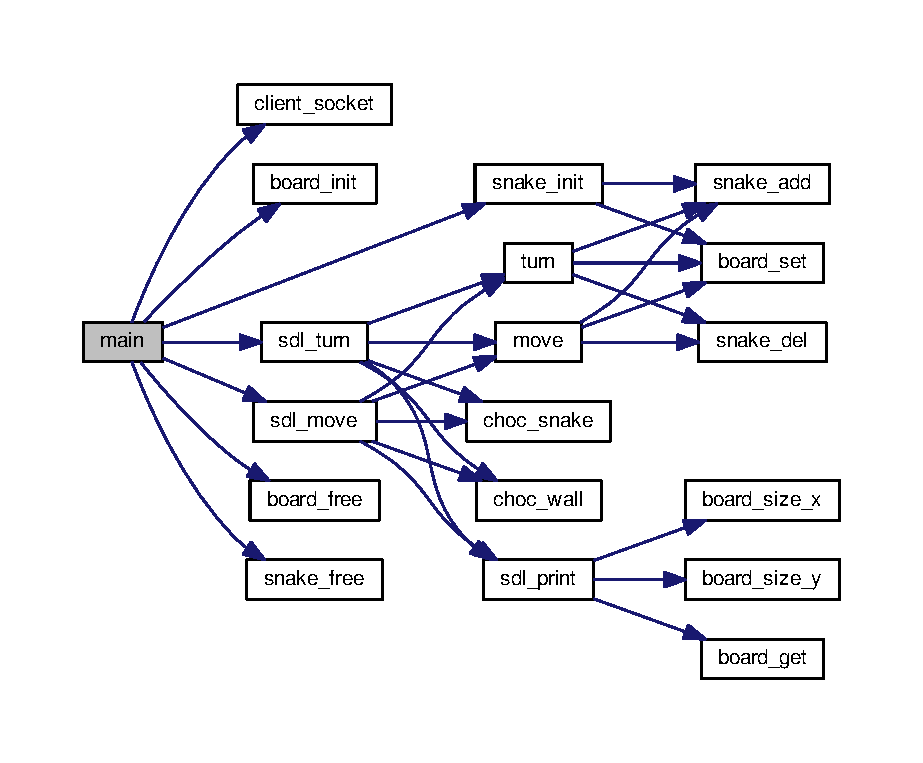
\includegraphics[width=350pt]{client_8c_ae66f6b31b5ad750f1fe042a706a4e3d4_cgraph}
\end{center}
\end{figure}


\index{client.\+c@{client.\+c}!sdl\+\_\+move@{sdl\+\_\+move}}
\index{sdl\+\_\+move@{sdl\+\_\+move}!client.\+c@{client.\+c}}
\subsubsection[{\texorpdfstring{sdl\+\_\+move()}{sdl_move()}}]{\setlength{\rightskip}{0pt plus 5cm}void $\ast$ sdl\+\_\+move (
\begin{DoxyParamCaption}
{}
\end{DoxyParamCaption}
)}\hypertarget{client_8c_af424c7fd4c84203cddfb7230bbe15401}{}\label{client_8c_af424c7fd4c84203cddfb7230bbe15401}

\begin{DoxyCode}
90 \{
91     \textcolor{keywordtype}{char} buff;
92     \textcolor{keywordflow}{while}(\hyperlink{client_8c_aab1bde286e010d81472b269b419806d6}{X})
93     \{
94         \textcolor{comment}{/* on ferme la variable mutex */}
95         pthread\_mutex\_lock(&\hyperlink{client_8c_a4acff8232e4aec9cd5c6dc200ac55ef3}{mutex});
96         \textcolor{comment}{/* move snake */}
97         \hyperlink{snakelib_8c_aa7c9d4fed2b3edb453a4501ba019dc00}{move}(&\hyperlink{client_8c_a20fdbd342281b7b5b77945c79d176b9f}{b},&\hyperlink{client_8c_a71e92e96b65208605aca57598cc827f1}{s},\hyperlink{client_8c_af6f0bd3dc13317f895c91323c25c2b8f}{t});
98         write(\hyperlink{client_8c_a76f11d9a0a47b94f72c2d0e77fb32240}{n},&\hyperlink{client_8c_a67668278838ab1eb0065ef9218c8de00}{m},1);
99         read(\hyperlink{client_8c_a76f11d9a0a47b94f72c2d0e77fb32240}{n},&buff,\textcolor{keyword}{sizeof}(\textcolor{keywordtype}{char}*));
100         \textcolor{keywordflow}{switch}(buff)
101         \{
102             \textcolor{keywordflow}{case} \textcolor{charliteral}{'m'}:
103                 \hyperlink{snakelib_8c_aa7c9d4fed2b3edb453a4501ba019dc00}{move}(&\hyperlink{client_8c_a20fdbd342281b7b5b77945c79d176b9f}{b},&\hyperlink{client_8c_aa6fd7c53c9b79f5a6ccb6f73b383263c}{c},\hyperlink{client_8c_a0318530b7ab3cba31a8e7213e34351cc}{o});
104                 \textcolor{keywordflow}{break};
105             \textcolor{keywordflow}{case} \textcolor{charliteral}{'l'}:
106                 \hyperlink{snakelib_8c_afa428ecb4385e08a82520bec11bafe36}{turn}(&\hyperlink{client_8c_a20fdbd342281b7b5b77945c79d176b9f}{b},&\hyperlink{client_8c_aa6fd7c53c9b79f5a6ccb6f73b383263c}{c},\hyperlink{client_8c_a0318530b7ab3cba31a8e7213e34351cc}{o},-1);
107                 \textcolor{keywordflow}{break};
108             \textcolor{keywordflow}{case} \textcolor{charliteral}{'r'}:
109                 \hyperlink{snakelib_8c_afa428ecb4385e08a82520bec11bafe36}{turn}(&\hyperlink{client_8c_a20fdbd342281b7b5b77945c79d176b9f}{b},&\hyperlink{client_8c_aa6fd7c53c9b79f5a6ccb6f73b383263c}{c},\hyperlink{client_8c_a0318530b7ab3cba31a8e7213e34351cc}{o},1);
110                 \textcolor{keywordflow}{break};
111         \}
112         \textcolor{comment}{/* affiche SDL */}
113         \textcolor{keywordflow}{if} ((\hyperlink{client_8c_aab1bde286e010d81472b269b419806d6}{X} = !(\hyperlink{snakelib_8c_ab96735ae82693727289ffe22fc940235}{choc\_snake}(&\hyperlink{client_8c_a71e92e96b65208605aca57598cc827f1}{s},&\hyperlink{client_8c_a71e92e96b65208605aca57598cc827f1}{s})) && !(\hyperlink{snakelib_8c_a50fa8a047abfa006a3371a94809e72c4}{choc\_wall}(&\hyperlink{client_8c_a20fdbd342281b7b5b77945c79d176b9f}{b},&
      \hyperlink{client_8c_a71e92e96b65208605aca57598cc827f1}{s}))))
114             \hyperlink{client_8c_a2cfeae643e415db24e85db6c4994b071}{sdl\_print}();
115         \textcolor{comment}{/* libere le mutex pour les autres thread */}
116         pthread\_mutex\_unlock(&\hyperlink{client_8c_a4acff8232e4aec9cd5c6dc200ac55ef3}{mutex});
117         \textcolor{comment}{/*u*/}sleep (1\textcolor{comment}{/*00000*/});
118     \}
119     pthread\_exit(0);
120 \}
\end{DoxyCode}


Voici le graphe d\textquotesingle{}appel pour cette fonction \+:\nopagebreak
\begin{figure}[H]
\begin{center}
\leavevmode
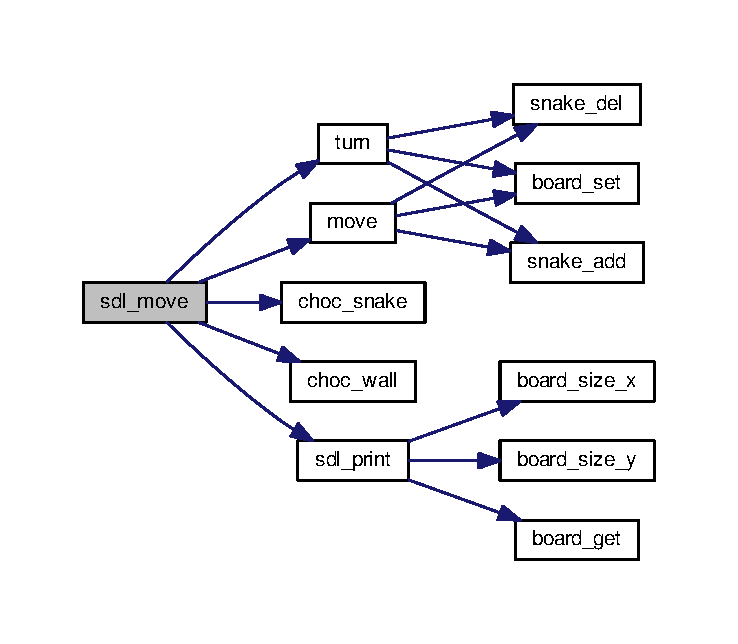
\includegraphics[width=350pt]{client_8c_af424c7fd4c84203cddfb7230bbe15401_cgraph}
\end{center}
\end{figure}




Voici le graphe des appelants de cette fonction \+:\nopagebreak
\begin{figure}[H]
\begin{center}
\leavevmode
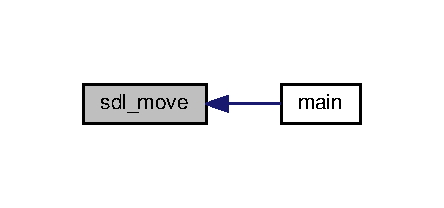
\includegraphics[width=213pt]{client_8c_af424c7fd4c84203cddfb7230bbe15401_icgraph}
\end{center}
\end{figure}


\index{client.\+c@{client.\+c}!sdl\+\_\+print@{sdl\+\_\+print}}
\index{sdl\+\_\+print@{sdl\+\_\+print}!client.\+c@{client.\+c}}
\subsubsection[{\texorpdfstring{sdl\+\_\+print()}{sdl_print()}}]{\setlength{\rightskip}{0pt plus 5cm}void sdl\+\_\+print (
\begin{DoxyParamCaption}
{}
\end{DoxyParamCaption}
)}\hypertarget{client_8c_a2cfeae643e415db24e85db6c4994b071}{}\label{client_8c_a2cfeae643e415db24e85db6c4994b071}

\begin{DoxyCode}
56                  \{
57     \textcolor{keywordtype}{int} x,y, dx = \hyperlink{snakelib_8c_ab6926a5a512798dea6aa52f5f15ab8ad}{board\_size\_x} (&\hyperlink{client_8c_a20fdbd342281b7b5b77945c79d176b9f}{b}), dy = \hyperlink{snakelib_8c_a01be021996158cf01e830b56e41be904}{board\_size\_y} (&
      \hyperlink{client_8c_a20fdbd342281b7b5b77945c79d176b9f}{b});
58     \textcolor{comment}{/* def une position */}
59     SDL\_Rect p;
60     \textcolor{keywordflow}{for} (x = 0; x < dx; x++)
61     \{
62         \textcolor{keywordflow}{for} (y = 0; y < dy; y++)
63         \{
64             p.x = x * 20 ; p.y = y * 20 ;
65             \textcolor{comment}{/* lire dans le plateau et dessiner la surface */}
66             \textcolor{keywordflow}{switch} (\hyperlink{snakelib_8c_ae49b60c78ec9b92e770c8eace9520447}{board\_get} (&\hyperlink{client_8c_a20fdbd342281b7b5b77945c79d176b9f}{b},x,y))
67             \{
68                 \textcolor{keywordflow}{case} \textcolor{charliteral}{'@'}:
69                     SDL\_BlitSurface(\hyperlink{client_8c_a79a54bef7bf02b18264c38fc90549a04}{A}, 0, \hyperlink{client_8c_ae8dfea36e66ed4b47c61a7ea5212e164}{E}, &p);
70                     \textcolor{keywordflow}{break};
71                 \textcolor{keywordflow}{case} \textcolor{charliteral}{' '}:
72                     SDL\_BlitSurface(\hyperlink{client_8c_ac54b5255531a4799123d0f8dca96a7cc}{B}, 0, \hyperlink{client_8c_ae8dfea36e66ed4b47c61a7ea5212e164}{E}, &p);
73                     \textcolor{keywordflow}{break};
74                 \textcolor{keywordflow}{case} \textcolor{charliteral}{'#'}:
75                     SDL\_BlitSurface(\hyperlink{client_8c_ab7d76262118cf1d4da44315136e542ca}{C}, 0, \hyperlink{client_8c_ae8dfea36e66ed4b47c61a7ea5212e164}{E}, &p);
76                     \textcolor{keywordflow}{break};
77                 \textcolor{keywordflow}{case} \textcolor{charliteral}{'&'}:
78                     SDL\_BlitSurface(\hyperlink{client_8c_aae9bd8b56defc5a6ec9c20b503b59a3a}{D}, 0, \hyperlink{client_8c_ae8dfea36e66ed4b47c61a7ea5212e164}{E}, &p);
79                     \textcolor{keywordflow}{break};
80             \}
81         \}
82     \}
83     \textcolor{comment}{/* reafficher un nouvelle ecran */}
84     SDL\_Flip(\hyperlink{client_8c_ae8dfea36e66ed4b47c61a7ea5212e164}{E});
85 \}
\end{DoxyCode}


Voici le graphe d\textquotesingle{}appel pour cette fonction \+:\nopagebreak
\begin{figure}[H]
\begin{center}
\leavevmode
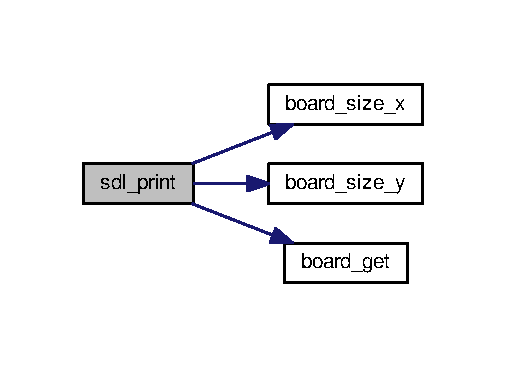
\includegraphics[width=243pt]{client_8c_a2cfeae643e415db24e85db6c4994b071_cgraph}
\end{center}
\end{figure}




Voici le graphe des appelants de cette fonction \+:\nopagebreak
\begin{figure}[H]
\begin{center}
\leavevmode
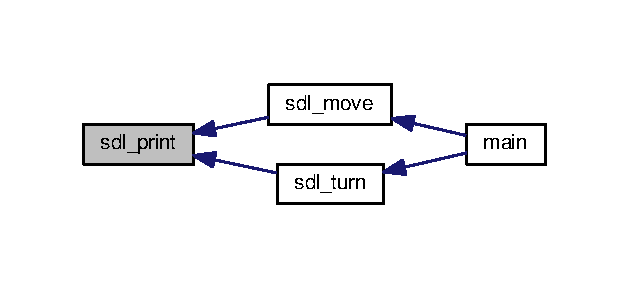
\includegraphics[width=302pt]{client_8c_a2cfeae643e415db24e85db6c4994b071_icgraph}
\end{center}
\end{figure}


\index{client.\+c@{client.\+c}!sdl\+\_\+turn@{sdl\+\_\+turn}}
\index{sdl\+\_\+turn@{sdl\+\_\+turn}!client.\+c@{client.\+c}}
\subsubsection[{\texorpdfstring{sdl\+\_\+turn()}{sdl_turn()}}]{\setlength{\rightskip}{0pt plus 5cm}void $\ast$ sdl\+\_\+turn (
\begin{DoxyParamCaption}
{}
\end{DoxyParamCaption}
)}\hypertarget{client_8c_ace514d3ea0e685be64430b930ef23b46}{}\label{client_8c_ace514d3ea0e685be64430b930ef23b46}

\begin{DoxyCode}
123 \{
124     SDL\_Event event;
125     \textcolor{keywordtype}{char} buff;
126     \textcolor{keywordflow}{while} (\hyperlink{client_8c_aab1bde286e010d81472b269b419806d6}{X})
127     \{
128     SDL\_WaitEvent(&event);
129         \textcolor{keywordflow}{switch} (event.type)
130         \{
131             \textcolor{keywordflow}{case} SDL\_QUIT:
132                 \hyperlink{client_8c_aab1bde286e010d81472b269b419806d6}{X} = \textcolor{keyword}{false};
133                 \textcolor{keywordflow}{break};
134             \textcolor{keywordflow}{case} SDL\_KEYDOWN:
135                 \textcolor{keywordflow}{switch} (event.key.keysym.sym)
136                 \{
137                     \textcolor{keywordflow}{case} SDLK\_ESCAPE:
138                         \hyperlink{client_8c_aab1bde286e010d81472b269b419806d6}{X} = \textcolor{keyword}{false};
139                         \textcolor{keywordflow}{break};
140                     \textcolor{keywordflow}{case} SDLK\_RIGHT:\textcolor{comment}{/* key right */}
141                     \textcolor{keywordflow}{case} SDLK\_KP3:\textcolor{comment}{/* keypad 3 */}
142                     \textcolor{keywordflow}{case} SDLK\_KP9:\textcolor{comment}{/* keypad 3 */}
143                     \textcolor{keywordflow}{case} \textcolor{charliteral}{'e'}:\textcolor{comment}{/* code ascii */}
144                         \textcolor{comment}{/* on ferme la variable mutex */}
145                         pthread\_mutex\_lock(&\hyperlink{client_8c_a4acff8232e4aec9cd5c6dc200ac55ef3}{mutex});
146                         \textcolor{comment}{/* turn snake */}
147                         \hyperlink{snakelib_8c_afa428ecb4385e08a82520bec11bafe36}{turn}(&\hyperlink{client_8c_a20fdbd342281b7b5b77945c79d176b9f}{b},&\hyperlink{client_8c_a71e92e96b65208605aca57598cc827f1}{s},1,\hyperlink{client_8c_af6f0bd3dc13317f895c91323c25c2b8f}{t});
148                         write(\hyperlink{client_8c_a76f11d9a0a47b94f72c2d0e77fb32240}{n},&\hyperlink{client_8c_a6edfa8f60e57212495b55b6b96c92cc5}{r},1);
149                         read(\hyperlink{client_8c_a76f11d9a0a47b94f72c2d0e77fb32240}{n},&buff,\textcolor{keyword}{sizeof}(\textcolor{keywordtype}{char}*));
150                         \textcolor{keywordflow}{switch}(buff)
151                         \{
152                             \textcolor{keywordflow}{case} \textcolor{charliteral}{'m'}:
153                                 \hyperlink{snakelib_8c_aa7c9d4fed2b3edb453a4501ba019dc00}{move}(&\hyperlink{client_8c_a20fdbd342281b7b5b77945c79d176b9f}{b},&\hyperlink{client_8c_aa6fd7c53c9b79f5a6ccb6f73b383263c}{c},\hyperlink{client_8c_a0318530b7ab3cba31a8e7213e34351cc}{o});
154                                 \textcolor{keywordflow}{break};
155                             \textcolor{keywordflow}{case} \textcolor{charliteral}{'l'}:
156                                 \hyperlink{snakelib_8c_afa428ecb4385e08a82520bec11bafe36}{turn}(&\hyperlink{client_8c_a20fdbd342281b7b5b77945c79d176b9f}{b},&\hyperlink{client_8c_aa6fd7c53c9b79f5a6ccb6f73b383263c}{c},\hyperlink{client_8c_a0318530b7ab3cba31a8e7213e34351cc}{o},-1);
157                                 \textcolor{keywordflow}{break};
158                             \textcolor{keywordflow}{case} \textcolor{charliteral}{'r'}:
159                                 \hyperlink{snakelib_8c_afa428ecb4385e08a82520bec11bafe36}{turn}(&\hyperlink{client_8c_a20fdbd342281b7b5b77945c79d176b9f}{b},&\hyperlink{client_8c_aa6fd7c53c9b79f5a6ccb6f73b383263c}{c},\hyperlink{client_8c_a0318530b7ab3cba31a8e7213e34351cc}{o},1);
160                                 \textcolor{keywordflow}{break};
161                         \}
162                         \textcolor{comment}{/* affiche SDL */}
163                         \textcolor{keywordflow}{if} ((\hyperlink{client_8c_aab1bde286e010d81472b269b419806d6}{X} = !(\hyperlink{snakelib_8c_ab96735ae82693727289ffe22fc940235}{choc\_snake}(&\hyperlink{client_8c_a71e92e96b65208605aca57598cc827f1}{s},&\hyperlink{client_8c_a71e92e96b65208605aca57598cc827f1}{s})) && !(
      \hyperlink{snakelib_8c_a50fa8a047abfa006a3371a94809e72c4}{choc\_wall}(&\hyperlink{client_8c_a20fdbd342281b7b5b77945c79d176b9f}{b},&\hyperlink{client_8c_a71e92e96b65208605aca57598cc827f1}{s}))))
164                             \hyperlink{client_8c_a2cfeae643e415db24e85db6c4994b071}{sdl\_print}();
165                         pthread\_mutex\_unlock(&\hyperlink{client_8c_a4acff8232e4aec9cd5c6dc200ac55ef3}{mutex});
166                         \textcolor{keywordflow}{break};
167                     \textcolor{keywordflow}{case} SDLK\_LEFT:\textcolor{comment}{/* key left */}
168                     \textcolor{keywordflow}{case} SDLK\_KP1:\textcolor{comment}{/* keypad 1*/}
169                     \textcolor{keywordflow}{case} SDLK\_KP7:\textcolor{comment}{/* keypad 7*/}
170                     \textcolor{keywordflow}{case} \textcolor{charliteral}{'a'}:\textcolor{comment}{/* code ascii */}
171                         \textcolor{comment}{/* on ferme la variable mutex */}
172                         pthread\_mutex\_lock(&\hyperlink{client_8c_a4acff8232e4aec9cd5c6dc200ac55ef3}{mutex});
173                         \textcolor{comment}{/* turn snake */}
174                         \hyperlink{snakelib_8c_afa428ecb4385e08a82520bec11bafe36}{turn}(&\hyperlink{client_8c_a20fdbd342281b7b5b77945c79d176b9f}{b},&\hyperlink{client_8c_a71e92e96b65208605aca57598cc827f1}{s},-1,\hyperlink{client_8c_af6f0bd3dc13317f895c91323c25c2b8f}{t});
175                         write(\hyperlink{client_8c_a76f11d9a0a47b94f72c2d0e77fb32240}{n},&\hyperlink{client_8c_a70893b9fd599f8c9ed3ed00c52eba44a}{l},1);
176                         read(\hyperlink{client_8c_a76f11d9a0a47b94f72c2d0e77fb32240}{n},&buff,\textcolor{keyword}{sizeof}(\textcolor{keywordtype}{char}*));
177                         \textcolor{keywordflow}{switch}(buff)
178                         \{
179                             \textcolor{keywordflow}{case} \textcolor{charliteral}{'m'}:
180                                 \hyperlink{snakelib_8c_aa7c9d4fed2b3edb453a4501ba019dc00}{move}(&\hyperlink{client_8c_a20fdbd342281b7b5b77945c79d176b9f}{b},&\hyperlink{client_8c_aa6fd7c53c9b79f5a6ccb6f73b383263c}{c},\hyperlink{client_8c_a0318530b7ab3cba31a8e7213e34351cc}{o});
181                                 \textcolor{keywordflow}{break};
182                             \textcolor{keywordflow}{case} \textcolor{charliteral}{'l'}:
183                                 \hyperlink{snakelib_8c_afa428ecb4385e08a82520bec11bafe36}{turn}(&\hyperlink{client_8c_a20fdbd342281b7b5b77945c79d176b9f}{b},&\hyperlink{client_8c_aa6fd7c53c9b79f5a6ccb6f73b383263c}{c},\hyperlink{client_8c_a0318530b7ab3cba31a8e7213e34351cc}{o},-1);
184                                 \textcolor{keywordflow}{break};
185                             \textcolor{keywordflow}{case} \textcolor{charliteral}{'r'}:
186                                 \hyperlink{snakelib_8c_afa428ecb4385e08a82520bec11bafe36}{turn}(&\hyperlink{client_8c_a20fdbd342281b7b5b77945c79d176b9f}{b},&\hyperlink{client_8c_aa6fd7c53c9b79f5a6ccb6f73b383263c}{c},\hyperlink{client_8c_a0318530b7ab3cba31a8e7213e34351cc}{o},1);
187                                 \textcolor{keywordflow}{break};
188                         \}
189                         \textcolor{comment}{/* affiche SDL */}
190                         \textcolor{keywordflow}{if} ((\hyperlink{client_8c_aab1bde286e010d81472b269b419806d6}{X} = !(\hyperlink{snakelib_8c_ab96735ae82693727289ffe22fc940235}{choc\_snake}(&\hyperlink{client_8c_a71e92e96b65208605aca57598cc827f1}{s},&\hyperlink{client_8c_a71e92e96b65208605aca57598cc827f1}{s})) && !(
      \hyperlink{snakelib_8c_a50fa8a047abfa006a3371a94809e72c4}{choc\_wall}(&\hyperlink{client_8c_a20fdbd342281b7b5b77945c79d176b9f}{b},&\hyperlink{client_8c_a71e92e96b65208605aca57598cc827f1}{s}))))
191                             \hyperlink{client_8c_a2cfeae643e415db24e85db6c4994b071}{sdl\_print}();
192                         \textcolor{comment}{/* libere le mutex pour les autres thread */}
193                         pthread\_mutex\_unlock(&\hyperlink{client_8c_a4acff8232e4aec9cd5c6dc200ac55ef3}{mutex});
194                         \textcolor{keywordflow}{break};
195                     \textcolor{keywordflow}{default}:\textcolor{comment}{/* ne fait rien */}\textcolor{keywordflow}{break};
196                 \}   
197             \textcolor{keywordflow}{default}:\textcolor{comment}{/* ne fait rien */}\textcolor{keywordflow}{break};
198         \}
199     \}
200     pthread\_exit(0);
201 \}
\end{DoxyCode}


Voici le graphe d\textquotesingle{}appel pour cette fonction \+:\nopagebreak
\begin{figure}[H]
\begin{center}
\leavevmode
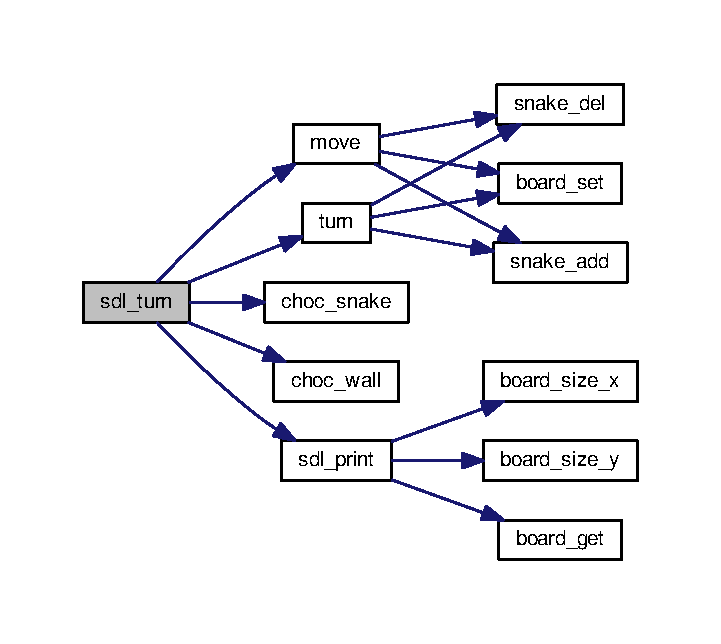
\includegraphics[width=346pt]{client_8c_ace514d3ea0e685be64430b930ef23b46_cgraph}
\end{center}
\end{figure}




Voici le graphe des appelants de cette fonction \+:\nopagebreak
\begin{figure}[H]
\begin{center}
\leavevmode
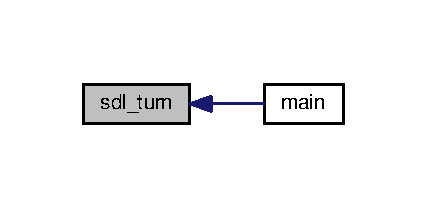
\includegraphics[width=205pt]{client_8c_ace514d3ea0e685be64430b930ef23b46_icgraph}
\end{center}
\end{figure}




\subsection{Documentation des variables}
\index{client.\+c@{client.\+c}!A@{A}}
\index{A@{A}!client.\+c@{client.\+c}}
\subsubsection[{\texorpdfstring{A}{A}}]{\setlength{\rightskip}{0pt plus 5cm}S\+D\+L\+\_\+\+Surface $\ast$ A}\hypertarget{client_8c_a79a54bef7bf02b18264c38fc90549a04}{}\label{client_8c_a79a54bef7bf02b18264c38fc90549a04}
\index{client.\+c@{client.\+c}!B@{B}}
\index{B@{B}!client.\+c@{client.\+c}}
\subsubsection[{\texorpdfstring{B}{B}}]{\setlength{\rightskip}{0pt plus 5cm}S\+D\+L\+\_\+\+Surface $\ast$ B}\hypertarget{client_8c_ac54b5255531a4799123d0f8dca96a7cc}{}\label{client_8c_ac54b5255531a4799123d0f8dca96a7cc}
\index{client.\+c@{client.\+c}!b@{b}}
\index{b@{b}!client.\+c@{client.\+c}}
\subsubsection[{\texorpdfstring{b}{b}}]{\setlength{\rightskip}{0pt plus 5cm}{\bf board} b}\hypertarget{client_8c_a20fdbd342281b7b5b77945c79d176b9f}{}\label{client_8c_a20fdbd342281b7b5b77945c79d176b9f}
\index{client.\+c@{client.\+c}!C@{C}}
\index{C@{C}!client.\+c@{client.\+c}}
\subsubsection[{\texorpdfstring{C}{C}}]{\setlength{\rightskip}{0pt plus 5cm}S\+D\+L\+\_\+\+Surface $\ast$ C}\hypertarget{client_8c_ab7d76262118cf1d4da44315136e542ca}{}\label{client_8c_ab7d76262118cf1d4da44315136e542ca}
\index{client.\+c@{client.\+c}!c@{c}}
\index{c@{c}!client.\+c@{client.\+c}}
\subsubsection[{\texorpdfstring{c}{c}}]{\setlength{\rightskip}{0pt plus 5cm}{\bf snake} c}\hypertarget{client_8c_aa6fd7c53c9b79f5a6ccb6f73b383263c}{}\label{client_8c_aa6fd7c53c9b79f5a6ccb6f73b383263c}
\index{client.\+c@{client.\+c}!D@{D}}
\index{D@{D}!client.\+c@{client.\+c}}
\subsubsection[{\texorpdfstring{D}{D}}]{\setlength{\rightskip}{0pt plus 5cm}S\+D\+L\+\_\+\+Surface $\ast$ D}\hypertarget{client_8c_aae9bd8b56defc5a6ec9c20b503b59a3a}{}\label{client_8c_aae9bd8b56defc5a6ec9c20b503b59a3a}
\index{client.\+c@{client.\+c}!E@{E}}
\index{E@{E}!client.\+c@{client.\+c}}
\subsubsection[{\texorpdfstring{E}{E}}]{\setlength{\rightskip}{0pt plus 5cm}S\+D\+L\+\_\+\+Surface$\ast$ E}\hypertarget{client_8c_ae8dfea36e66ed4b47c61a7ea5212e164}{}\label{client_8c_ae8dfea36e66ed4b47c61a7ea5212e164}
\index{client.\+c@{client.\+c}!l@{l}}
\index{l@{l}!client.\+c@{client.\+c}}
\subsubsection[{\texorpdfstring{l}{l}}]{\setlength{\rightskip}{0pt plus 5cm}char l}\hypertarget{client_8c_a70893b9fd599f8c9ed3ed00c52eba44a}{}\label{client_8c_a70893b9fd599f8c9ed3ed00c52eba44a}
\index{client.\+c@{client.\+c}!m@{m}}
\index{m@{m}!client.\+c@{client.\+c}}
\subsubsection[{\texorpdfstring{m}{m}}]{\setlength{\rightskip}{0pt plus 5cm}char m}\hypertarget{client_8c_a67668278838ab1eb0065ef9218c8de00}{}\label{client_8c_a67668278838ab1eb0065ef9218c8de00}
\index{client.\+c@{client.\+c}!mutex@{mutex}}
\index{mutex@{mutex}!client.\+c@{client.\+c}}
\subsubsection[{\texorpdfstring{mutex}{mutex}}]{\setlength{\rightskip}{0pt plus 5cm}pthread\+\_\+mutex\+\_\+t mutex = P\+T\+H\+R\+E\+A\+D\+\_\+\+M\+U\+T\+E\+X\+\_\+\+I\+N\+I\+T\+I\+A\+L\+I\+Z\+ER}\hypertarget{client_8c_a4acff8232e4aec9cd5c6dc200ac55ef3}{}\label{client_8c_a4acff8232e4aec9cd5c6dc200ac55ef3}
\index{client.\+c@{client.\+c}!n@{n}}
\index{n@{n}!client.\+c@{client.\+c}}
\subsubsection[{\texorpdfstring{n}{n}}]{\setlength{\rightskip}{0pt plus 5cm}int n}\hypertarget{client_8c_a76f11d9a0a47b94f72c2d0e77fb32240}{}\label{client_8c_a76f11d9a0a47b94f72c2d0e77fb32240}
\index{client.\+c@{client.\+c}!o@{o}}
\index{o@{o}!client.\+c@{client.\+c}}
\subsubsection[{\texorpdfstring{o}{o}}]{\setlength{\rightskip}{0pt plus 5cm}char o}\hypertarget{client_8c_a0318530b7ab3cba31a8e7213e34351cc}{}\label{client_8c_a0318530b7ab3cba31a8e7213e34351cc}
\index{client.\+c@{client.\+c}!r@{r}}
\index{r@{r}!client.\+c@{client.\+c}}
\subsubsection[{\texorpdfstring{r}{r}}]{\setlength{\rightskip}{0pt plus 5cm}char r}\hypertarget{client_8c_a6edfa8f60e57212495b55b6b96c92cc5}{}\label{client_8c_a6edfa8f60e57212495b55b6b96c92cc5}
\index{client.\+c@{client.\+c}!s@{s}}
\index{s@{s}!client.\+c@{client.\+c}}
\subsubsection[{\texorpdfstring{s}{s}}]{\setlength{\rightskip}{0pt plus 5cm}{\bf snake} s}\hypertarget{client_8c_a71e92e96b65208605aca57598cc827f1}{}\label{client_8c_a71e92e96b65208605aca57598cc827f1}
\index{client.\+c@{client.\+c}!t@{t}}
\index{t@{t}!client.\+c@{client.\+c}}
\subsubsection[{\texorpdfstring{t}{t}}]{\setlength{\rightskip}{0pt plus 5cm}char t}\hypertarget{client_8c_af6f0bd3dc13317f895c91323c25c2b8f}{}\label{client_8c_af6f0bd3dc13317f895c91323c25c2b8f}
\index{client.\+c@{client.\+c}!threadpt@{threadpt}}
\index{threadpt@{threadpt}!client.\+c@{client.\+c}}
\subsubsection[{\texorpdfstring{threadpt}{threadpt}}]{\setlength{\rightskip}{0pt plus 5cm}pthread\+\_\+t threadpt}\hypertarget{client_8c_acdb501237bbfd1adad2d00fc7052a767}{}\label{client_8c_acdb501237bbfd1adad2d00fc7052a767}
\index{client.\+c@{client.\+c}!X@{X}}
\index{X@{X}!client.\+c@{client.\+c}}
\subsubsection[{\texorpdfstring{X}{X}}]{\setlength{\rightskip}{0pt plus 5cm}bool X}\hypertarget{client_8c_aab1bde286e010d81472b269b419806d6}{}\label{client_8c_aab1bde286e010d81472b269b419806d6}

\hypertarget{schlanga_8c}{}\section{Référence du fichier S\+O\+U\+R\+C\+E/schlanga.c}
\label{schlanga_8c}\index{S\+O\+U\+R\+C\+E/schlanga.\+c@{S\+O\+U\+R\+C\+E/schlanga.\+c}}
{\ttfamily \#include \char`\"{}../\+I\+N\+C\+L\+U\+D\+E/snakelib.\+h\char`\"{}}\\*
{\ttfamily \#include \char`\"{}../\+I\+N\+C\+L\+U\+D\+E/schlangalib.\+h\char`\"{}}\\*
{\ttfamily \#include $<$S\+D\+L/\+S\+D\+L.\+h$>$}\\*
{\ttfamily \#include $<$pthread.\+h$>$}\\*
{\ttfamily \#include $<$stdbool.\+h$>$}\\*
{\ttfamily \#include $<$unistd.\+h$>$}\\*
{\ttfamily \#include $<$time.\+h$>$}\\*
Graphe des dépendances par inclusion de schlanga.\+c\+:\nopagebreak
\begin{figure}[H]
\begin{center}
\leavevmode
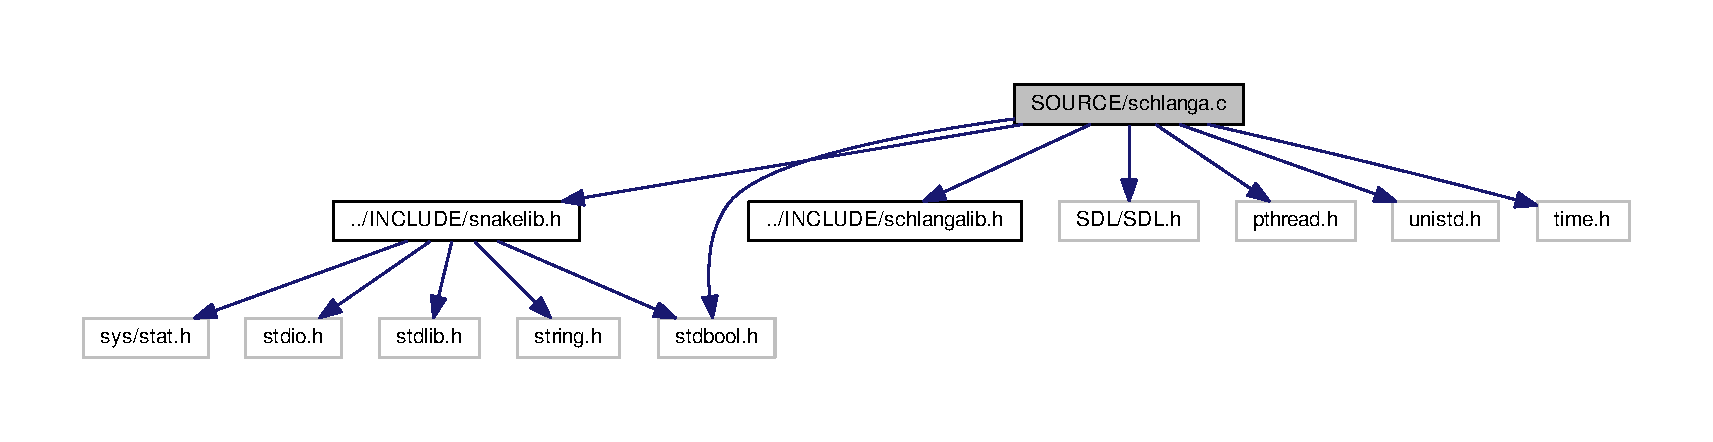
\includegraphics[width=350pt]{schlanga_8c__incl}
\end{center}
\end{figure}
\subsection*{Macros}
\begin{DoxyCompactItemize}
\item 
\#define \hyperlink{schlanga_8c_aa9e0582fb2da4f96cb13bf68a6a9f073}{B\+O\+A\+R\+D\+\_\+\+S\+I\+Z\+E\+\_\+X}~68
\item 
\#define \hyperlink{schlanga_8c_acfabc043baaf3c01ee67a77c2ae6b078}{B\+O\+A\+R\+D\+\_\+\+S\+I\+Z\+E\+\_\+Y}~33
\item 
\#define \hyperlink{schlanga_8c_a37a78e9845fe459f5a2be9fe6ce52d24}{S\+N\+A\+K\+E\+\_\+\+L\+EN}~12
\item 
\#define \hyperlink{schlanga_8c_a44e89d523436fcbbf2c56e4fb335d509}{S\+L\+E\+EP}~105000
\end{DoxyCompactItemize}
\subsection*{Fonctions}
\begin{DoxyCompactItemize}
\item 
void $\ast$ \hyperlink{schlanga_8c_ab6f22cbb52dc4a7603d7c42a3521a7c6}{sdl\+\_\+turn} ()
\item 
void $\ast$ \hyperlink{schlanga_8c_aa4bd8217532482639db456d8d6a59598}{sdl\+\_\+move} ()
\item 
void \hyperlink{schlanga_8c_a2cfeae643e415db24e85db6c4994b071}{sdl\+\_\+print} ()
\item 
int \hyperlink{schlanga_8c_ae66f6b31b5ad750f1fe042a706a4e3d4}{main} ()
\end{DoxyCompactItemize}
\subsection*{Variables}
\begin{DoxyCompactItemize}
\item 
pthread\+\_\+mutex\+\_\+t \hyperlink{schlanga_8c_a4acff8232e4aec9cd5c6dc200ac55ef3}{mutex} = P\+T\+H\+R\+E\+A\+D\+\_\+\+M\+U\+T\+E\+X\+\_\+\+I\+N\+I\+T\+I\+A\+L\+I\+Z\+ER
\item 
bool \hyperlink{schlanga_8c_aab1bde286e010d81472b269b419806d6}{X}
\item 
S\+D\+L\+\_\+\+Surface $\ast$ \hyperlink{schlanga_8c_ae8dfea36e66ed4b47c61a7ea5212e164}{E}
\item 
S\+D\+L\+\_\+\+Surface $\ast$ \hyperlink{schlanga_8c_a79a54bef7bf02b18264c38fc90549a04}{A}
\item 
S\+D\+L\+\_\+\+Surface $\ast$ \hyperlink{schlanga_8c_ac54b5255531a4799123d0f8dca96a7cc}{B}
\item 
S\+D\+L\+\_\+\+Surface $\ast$ \hyperlink{schlanga_8c_ab7d76262118cf1d4da44315136e542ca}{C}
\item 
S\+D\+L\+\_\+\+Surface $\ast$ \hyperlink{schlanga_8c_aae9bd8b56defc5a6ec9c20b503b59a3a}{D}
\item 
\hyperlink{structboard}{board} \hyperlink{schlanga_8c_a20fdbd342281b7b5b77945c79d176b9f}{b}
\item 
\hyperlink{structsnake}{snake} \hyperlink{schlanga_8c_a71e92e96b65208605aca57598cc827f1}{s}
\item 
\hyperlink{structsnake}{snake} \hyperlink{schlanga_8c_aa6fd7c53c9b79f5a6ccb6f73b383263c}{c}
\end{DoxyCompactItemize}


\subsection{Documentation des macros}
\index{schlanga.\+c@{schlanga.\+c}!B\+O\+A\+R\+D\+\_\+\+S\+I\+Z\+E\+\_\+X@{B\+O\+A\+R\+D\+\_\+\+S\+I\+Z\+E\+\_\+X}}
\index{B\+O\+A\+R\+D\+\_\+\+S\+I\+Z\+E\+\_\+X@{B\+O\+A\+R\+D\+\_\+\+S\+I\+Z\+E\+\_\+X}!schlanga.\+c@{schlanga.\+c}}
\subsubsection[{\texorpdfstring{B\+O\+A\+R\+D\+\_\+\+S\+I\+Z\+E\+\_\+X}{BOARD_SIZE_X}}]{\setlength{\rightskip}{0pt plus 5cm}\#define B\+O\+A\+R\+D\+\_\+\+S\+I\+Z\+E\+\_\+X~68}\hypertarget{schlanga_8c_aa9e0582fb2da4f96cb13bf68a6a9f073}{}\label{schlanga_8c_aa9e0582fb2da4f96cb13bf68a6a9f073}
\index{schlanga.\+c@{schlanga.\+c}!B\+O\+A\+R\+D\+\_\+\+S\+I\+Z\+E\+\_\+Y@{B\+O\+A\+R\+D\+\_\+\+S\+I\+Z\+E\+\_\+Y}}
\index{B\+O\+A\+R\+D\+\_\+\+S\+I\+Z\+E\+\_\+Y@{B\+O\+A\+R\+D\+\_\+\+S\+I\+Z\+E\+\_\+Y}!schlanga.\+c@{schlanga.\+c}}
\subsubsection[{\texorpdfstring{B\+O\+A\+R\+D\+\_\+\+S\+I\+Z\+E\+\_\+Y}{BOARD_SIZE_Y}}]{\setlength{\rightskip}{0pt plus 5cm}\#define B\+O\+A\+R\+D\+\_\+\+S\+I\+Z\+E\+\_\+Y~33}\hypertarget{schlanga_8c_acfabc043baaf3c01ee67a77c2ae6b078}{}\label{schlanga_8c_acfabc043baaf3c01ee67a77c2ae6b078}
\index{schlanga.\+c@{schlanga.\+c}!S\+L\+E\+EP@{S\+L\+E\+EP}}
\index{S\+L\+E\+EP@{S\+L\+E\+EP}!schlanga.\+c@{schlanga.\+c}}
\subsubsection[{\texorpdfstring{S\+L\+E\+EP}{SLEEP}}]{\setlength{\rightskip}{0pt plus 5cm}\#define S\+L\+E\+EP~105000}\hypertarget{schlanga_8c_a44e89d523436fcbbf2c56e4fb335d509}{}\label{schlanga_8c_a44e89d523436fcbbf2c56e4fb335d509}
\index{schlanga.\+c@{schlanga.\+c}!S\+N\+A\+K\+E\+\_\+\+L\+EN@{S\+N\+A\+K\+E\+\_\+\+L\+EN}}
\index{S\+N\+A\+K\+E\+\_\+\+L\+EN@{S\+N\+A\+K\+E\+\_\+\+L\+EN}!schlanga.\+c@{schlanga.\+c}}
\subsubsection[{\texorpdfstring{S\+N\+A\+K\+E\+\_\+\+L\+EN}{SNAKE_LEN}}]{\setlength{\rightskip}{0pt plus 5cm}\#define S\+N\+A\+K\+E\+\_\+\+L\+EN~12}\hypertarget{schlanga_8c_a37a78e9845fe459f5a2be9fe6ce52d24}{}\label{schlanga_8c_a37a78e9845fe459f5a2be9fe6ce52d24}


\subsection{Documentation des fonctions}
\index{schlanga.\+c@{schlanga.\+c}!main@{main}}
\index{main@{main}!schlanga.\+c@{schlanga.\+c}}
\subsubsection[{\texorpdfstring{main()}{main()}}]{\setlength{\rightskip}{0pt plus 5cm}int main (
\begin{DoxyParamCaption}
{}
\end{DoxyParamCaption}
)}\hypertarget{schlanga_8c_ae66f6b31b5ad750f1fe042a706a4e3d4}{}\label{schlanga_8c_ae66f6b31b5ad750f1fe042a706a4e3d4}

\begin{DoxyCode}
26 \{
27     \textcolor{comment}{/* rand init */}
28     srand(time(0));
29     \hyperlink{schlanga_8c_aab1bde286e010d81472b269b419806d6}{X} = \textcolor{keyword}{true};
30     \textcolor{comment}{/* init board + snake */}
31     \hyperlink{schlanga_8c_a20fdbd342281b7b5b77945c79d176b9f}{b} = \hyperlink{snakelib_8c_a9625331c000178d2cf90ef40d2a8fbf7}{board\_init}(\hyperlink{schlanga_8c_aa9e0582fb2da4f96cb13bf68a6a9f073}{BOARD\_SIZE\_X},\hyperlink{schlanga_8c_acfabc043baaf3c01ee67a77c2ae6b078}{BOARD\_SIZE\_Y});
32     \hyperlink{snakelib_8c_ac696fcc76930ea0badb2f263dd479c93}{snake\_init}(&\hyperlink{schlanga_8c_a20fdbd342281b7b5b77945c79d176b9f}{b},&\hyperlink{schlanga_8c_a71e92e96b65208605aca57598cc827f1}{s},\hyperlink{schlanga_8c_a37a78e9845fe459f5a2be9fe6ce52d24}{SNAKE\_LEN},\textcolor{charliteral}{'@'});
33     \hyperlink{snakelib_8c_ac696fcc76930ea0badb2f263dd479c93}{snake\_init}(&\hyperlink{schlanga_8c_a20fdbd342281b7b5b77945c79d176b9f}{b},&\hyperlink{schlanga_8c_aa6fd7c53c9b79f5a6ccb6f73b383263c}{c},\hyperlink{schlanga_8c_a37a78e9845fe459f5a2be9fe6ce52d24}{SNAKE\_LEN},\textcolor{charliteral}{'&'});
34     \textcolor{comment}{/* init sdl en mode video */}
35     SDL\_Init(SDL\_INIT\_VIDEO);
36     \textcolor{comment}{/* init surface E avec une taille 20*BOARD\_SIZE\_X et 20*BOARD\_SIZE\_Y */}
37     \hyperlink{schlanga_8c_ae8dfea36e66ed4b47c61a7ea5212e164}{E} = SDL\_SetVideoMode(20*\hyperlink{schlanga_8c_aa9e0582fb2da4f96cb13bf68a6a9f073}{BOARD\_SIZE\_X}, 20*\hyperlink{schlanga_8c_acfabc043baaf3c01ee67a77c2ae6b078}{BOARD\_SIZE\_Y}, 32, SDL\_HWSURFACE);
38     \textcolor{comment}{/* creer le reste des surfaces avec une taille de 20*20 px */}
39     \hyperlink{schlanga_8c_a79a54bef7bf02b18264c38fc90549a04}{A} = SDL\_CreateRGBSurface(SDL\_HWSURFACE, 20, 20, 32, 0, 0, 0, 0);
40     \hyperlink{schlanga_8c_ac54b5255531a4799123d0f8dca96a7cc}{B} = SDL\_CreateRGBSurface(SDL\_HWSURFACE, 20, 20, 32, 0, 0, 0, 0);
41     \hyperlink{schlanga_8c_ab7d76262118cf1d4da44315136e542ca}{C} = SDL\_CreateRGBSurface(SDL\_HWSURFACE, 20, 20, 32, 0, 0, 0, 0);
42     \hyperlink{schlanga_8c_aae9bd8b56defc5a6ec9c20b503b59a3a}{D} = SDL\_CreateRGBSurface(SDL\_HWSURFACE, 20, 20, 32, 0, 0, 0, 0);
43     \textcolor{comment}{/* init avec couleur rgb */}
44     SDL\_FillRect(\hyperlink{schlanga_8c_a79a54bef7bf02b18264c38fc90549a04}{A}, 0, SDL\_MapRGB(\hyperlink{schlanga_8c_ae8dfea36e66ed4b47c61a7ea5212e164}{E}->format, 95, 0, 0));
45     SDL\_FillRect(\hyperlink{schlanga_8c_ac54b5255531a4799123d0f8dca96a7cc}{B}, 0, SDL\_MapRGB(\hyperlink{schlanga_8c_ae8dfea36e66ed4b47c61a7ea5212e164}{E}->format, 137, 137, 137));
46     SDL\_FillRect(\hyperlink{schlanga_8c_ab7d76262118cf1d4da44315136e542ca}{C}, 0, SDL\_MapRGB(\hyperlink{schlanga_8c_ae8dfea36e66ed4b47c61a7ea5212e164}{E}->format, 47, 47, 47));
47     SDL\_FillRect(\hyperlink{schlanga_8c_aae9bd8b56defc5a6ec9c20b503b59a3a}{D}, 0, SDL\_MapRGB(\hyperlink{schlanga_8c_ae8dfea36e66ed4b47c61a7ea5212e164}{E}->format, 157, 62, 12));
48     \textcolor{comment}{/* init barre de fenetre */}
49     SDL\_WM\_SetCaption(\textcolor{stringliteral}{"Snack"}, 0);
50     \textcolor{comment}{/* nos variabe de thread */}
51     pthread\_t thread\_turn;
52     pthread\_t thread\_move;
53     \textcolor{comment}{/* creer les thread */}
54     pthread\_create(&thread\_turn, 0, &\hyperlink{schlanga_8c_ab6f22cbb52dc4a7603d7c42a3521a7c6}{sdl\_turn}, 0);
55     pthread\_create(&thread\_move, 0, &\hyperlink{schlanga_8c_aa4bd8217532482639db456d8d6a59598}{sdl\_move},0);
56     \textcolor{comment}{/* attendre leurs fin */}
57     pthread\_join(thread\_turn, 0);
58     pthread\_join(thread\_move, 0);
59     \textcolor{comment}{/* libere surface */}
60     SDL\_FreeSurface(\hyperlink{schlanga_8c_ae8dfea36e66ed4b47c61a7ea5212e164}{E});
61     SDL\_FreeSurface(\hyperlink{schlanga_8c_a79a54bef7bf02b18264c38fc90549a04}{A});
62     SDL\_FreeSurface(\hyperlink{schlanga_8c_ac54b5255531a4799123d0f8dca96a7cc}{B});
63     SDL\_FreeSurface(\hyperlink{schlanga_8c_ab7d76262118cf1d4da44315136e542ca}{C});
64     \textcolor{comment}{/* libere board + snake */}
65     \hyperlink{snakelib_8c_a223ea5e585467eee652b6b3b7a59e0c9}{board\_free}(&\hyperlink{schlanga_8c_a20fdbd342281b7b5b77945c79d176b9f}{b});
66     \hyperlink{snakelib_8c_ae2b728ff11f9b12d88715ddef95639c9}{snake\_free}(&\hyperlink{schlanga_8c_a71e92e96b65208605aca57598cc827f1}{s});
67     \hyperlink{snakelib_8c_ae2b728ff11f9b12d88715ddef95639c9}{snake\_free}(&\hyperlink{schlanga_8c_aa6fd7c53c9b79f5a6ccb6f73b383263c}{c});
68     SDL\_Quit();
69     \textcolor{keywordflow}{return} 0;
70 \}
\end{DoxyCode}


Voici le graphe d\textquotesingle{}appel pour cette fonction \+:\nopagebreak
\begin{figure}[H]
\begin{center}
\leavevmode
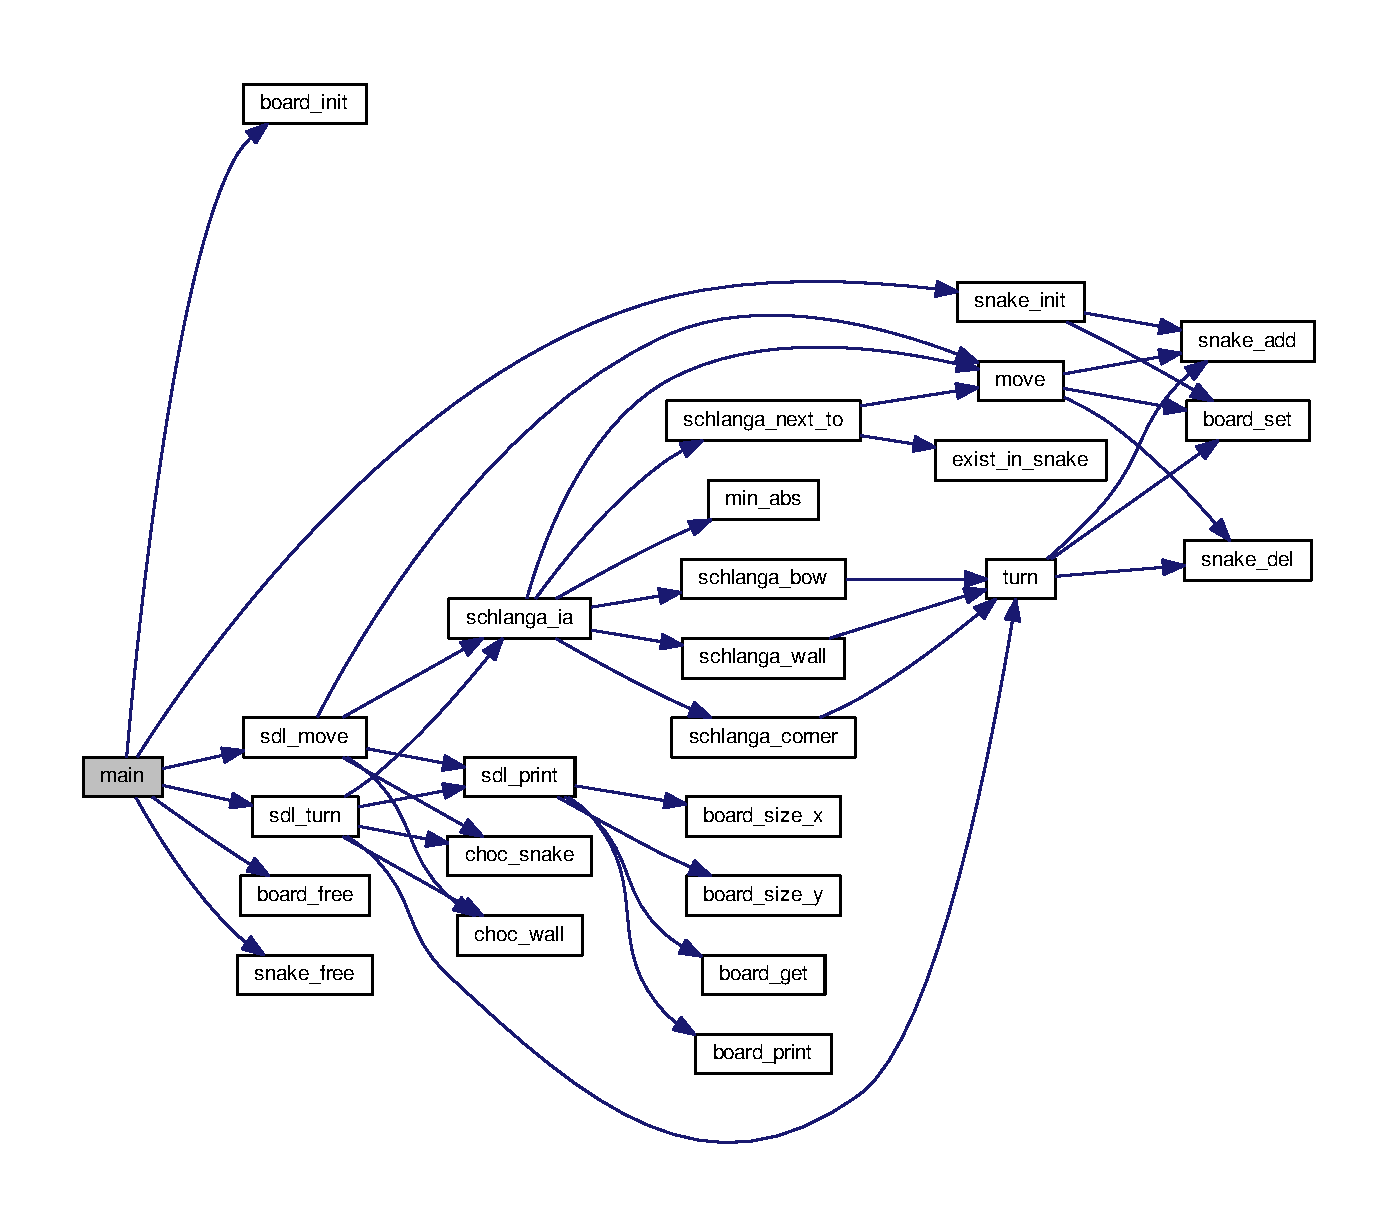
\includegraphics[width=350pt]{schlanga_8c_ae66f6b31b5ad750f1fe042a706a4e3d4_cgraph}
\end{center}
\end{figure}


\index{schlanga.\+c@{schlanga.\+c}!sdl\+\_\+move@{sdl\+\_\+move}}
\index{sdl\+\_\+move@{sdl\+\_\+move}!schlanga.\+c@{schlanga.\+c}}
\subsubsection[{\texorpdfstring{sdl\+\_\+move()}{sdl_move()}}]{\setlength{\rightskip}{0pt plus 5cm}void$\ast$ sdl\+\_\+move (
\begin{DoxyParamCaption}
{}
\end{DoxyParamCaption}
)}\hypertarget{schlanga_8c_aa4bd8217532482639db456d8d6a59598}{}\label{schlanga_8c_aa4bd8217532482639db456d8d6a59598}

\begin{DoxyCode}
145 \{
146     \textcolor{keywordflow}{while}(\hyperlink{schlanga_8c_aab1bde286e010d81472b269b419806d6}{X}) 
147     \{
148             \textcolor{comment}{/* on ferme la variable mutex */}
149             pthread\_mutex\_lock(&\hyperlink{schlanga_8c_a4acff8232e4aec9cd5c6dc200ac55ef3}{mutex});
150             \textcolor{comment}{/* move snake */}
151             \hyperlink{snakelib_8c_aa7c9d4fed2b3edb453a4501ba019dc00}{move}(&\hyperlink{schlanga_8c_a20fdbd342281b7b5b77945c79d176b9f}{b},&\hyperlink{schlanga_8c_a71e92e96b65208605aca57598cc827f1}{s},\textcolor{charliteral}{'@'});
152             \hyperlink{schlangalib_8c_a28adbac02fbdf8816543c25878bfd81d}{schlanga\_ia}(&\hyperlink{schlanga_8c_a20fdbd342281b7b5b77945c79d176b9f}{b},&\hyperlink{schlanga_8c_a71e92e96b65208605aca57598cc827f1}{s},&\hyperlink{schlanga_8c_aa6fd7c53c9b79f5a6ccb6f73b383263c}{c},\hyperlink{schlanga_8c_a37a78e9845fe459f5a2be9fe6ce52d24}{SNAKE\_LEN});
153             \textcolor{keywordflow}{if} ((\hyperlink{schlanga_8c_aab1bde286e010d81472b269b419806d6}{X} = !(\hyperlink{snakelib_8c_ab96735ae82693727289ffe22fc940235}{choc\_snake}(&\hyperlink{schlanga_8c_a71e92e96b65208605aca57598cc827f1}{s},&\hyperlink{schlanga_8c_a71e92e96b65208605aca57598cc827f1}{s}))\(\backslash\)
154                 && !(\hyperlink{snakelib_8c_a50fa8a047abfa006a3371a94809e72c4}{choc\_wall}(&\hyperlink{schlanga_8c_a20fdbd342281b7b5b77945c79d176b9f}{b},&\hyperlink{schlanga_8c_a71e92e96b65208605aca57598cc827f1}{s}))\(\backslash\)
155                 && !(\hyperlink{snakelib_8c_ab96735ae82693727289ffe22fc940235}{choc\_snake}(&\hyperlink{schlanga_8c_aa6fd7c53c9b79f5a6ccb6f73b383263c}{c},&\hyperlink{schlanga_8c_aa6fd7c53c9b79f5a6ccb6f73b383263c}{c}))\(\backslash\)
156                 && !(\hyperlink{snakelib_8c_a50fa8a047abfa006a3371a94809e72c4}{choc\_wall}(&\hyperlink{schlanga_8c_a20fdbd342281b7b5b77945c79d176b9f}{b},&\hyperlink{schlanga_8c_aa6fd7c53c9b79f5a6ccb6f73b383263c}{c}))\(\backslash\)
157                 && !(\hyperlink{snakelib_8c_ab96735ae82693727289ffe22fc940235}{choc\_snake}(&\hyperlink{schlanga_8c_aa6fd7c53c9b79f5a6ccb6f73b383263c}{c},&\hyperlink{schlanga_8c_a71e92e96b65208605aca57598cc827f1}{s}))\(\backslash\)
158                 && !(\hyperlink{snakelib_8c_ab96735ae82693727289ffe22fc940235}{choc\_snake}(&\hyperlink{schlanga_8c_a71e92e96b65208605aca57598cc827f1}{s},&\hyperlink{schlanga_8c_aa6fd7c53c9b79f5a6ccb6f73b383263c}{c}))))
159             
160             \{
161                 \hyperlink{schlanga_8c_a2cfeae643e415db24e85db6c4994b071}{sdl\_print}();
162             \}
163             \textcolor{comment}{/* libere le mutex pour les autres thread */}
164             pthread\_mutex\_unlock(&\hyperlink{schlanga_8c_a4acff8232e4aec9cd5c6dc200ac55ef3}{mutex});
165             usleep(\hyperlink{schlanga_8c_a44e89d523436fcbbf2c56e4fb335d509}{SLEEP});
166         \}
167         pthread\_exit(0);
168 \}
\end{DoxyCode}


Voici le graphe d\textquotesingle{}appel pour cette fonction \+:\nopagebreak
\begin{figure}[H]
\begin{center}
\leavevmode
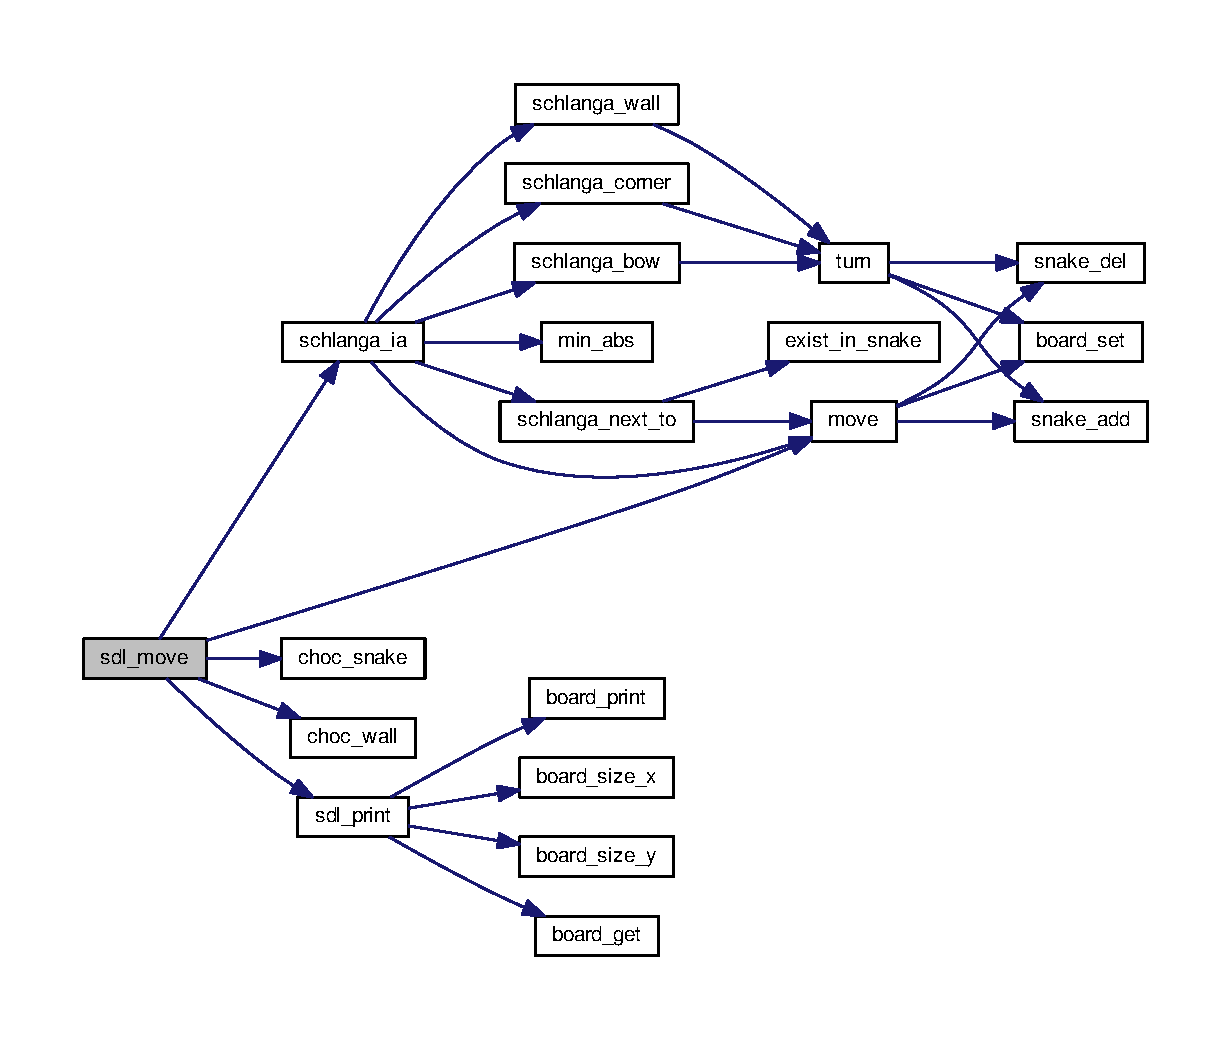
\includegraphics[width=350pt]{schlanga_8c_aa4bd8217532482639db456d8d6a59598_cgraph}
\end{center}
\end{figure}




Voici le graphe des appelants de cette fonction \+:\nopagebreak
\begin{figure}[H]
\begin{center}
\leavevmode
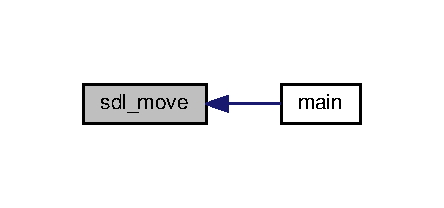
\includegraphics[width=213pt]{schlanga_8c_aa4bd8217532482639db456d8d6a59598_icgraph}
\end{center}
\end{figure}


\index{schlanga.\+c@{schlanga.\+c}!sdl\+\_\+print@{sdl\+\_\+print}}
\index{sdl\+\_\+print@{sdl\+\_\+print}!schlanga.\+c@{schlanga.\+c}}
\subsubsection[{\texorpdfstring{sdl\+\_\+print()}{sdl_print()}}]{\setlength{\rightskip}{0pt plus 5cm}void sdl\+\_\+print (
\begin{DoxyParamCaption}
{}
\end{DoxyParamCaption}
)}\hypertarget{schlanga_8c_a2cfeae643e415db24e85db6c4994b071}{}\label{schlanga_8c_a2cfeae643e415db24e85db6c4994b071}

\begin{DoxyCode}
173 \{
174     \textcolor{keywordtype}{int} x,y, dx = \hyperlink{snakelib_8c_ab6926a5a512798dea6aa52f5f15ab8ad}{board\_size\_x} (&\hyperlink{schlanga_8c_a20fdbd342281b7b5b77945c79d176b9f}{b}), dy = \hyperlink{snakelib_8c_a01be021996158cf01e830b56e41be904}{board\_size\_y} (&
      \hyperlink{schlanga_8c_a20fdbd342281b7b5b77945c79d176b9f}{b});
175     \textcolor{comment}{/* def une position */}
176     SDL\_Rect p;
177     \textcolor{keywordflow}{for} (x = 0; x < dx; x++) 
178     \{
179         \textcolor{keywordflow}{for} (y = 0; y < dy; y++) 
180         \{
181             p.x = x * 20 ; p.y = y * 20 ;
182             \textcolor{comment}{/* lire dans le plateau et dessiner la surface */}
183             \textcolor{keywordflow}{switch} (\hyperlink{snakelib_8c_ae49b60c78ec9b92e770c8eace9520447}{board\_get} (&\hyperlink{schlanga_8c_a20fdbd342281b7b5b77945c79d176b9f}{b},x,y)) 
184             \{
185                 \textcolor{keywordflow}{case} \textcolor{charliteral}{'@'}:
186                     SDL\_BlitSurface(\hyperlink{schlanga_8c_a79a54bef7bf02b18264c38fc90549a04}{A}, 0, \hyperlink{schlanga_8c_ae8dfea36e66ed4b47c61a7ea5212e164}{E}, &p);
187                     \textcolor{keywordflow}{break};
188                 \textcolor{keywordflow}{case} \textcolor{charliteral}{' '}:
189                     SDL\_BlitSurface(\hyperlink{schlanga_8c_ac54b5255531a4799123d0f8dca96a7cc}{B}, 0, \hyperlink{schlanga_8c_ae8dfea36e66ed4b47c61a7ea5212e164}{E}, &p);
190                     \textcolor{keywordflow}{break};
191                 \textcolor{keywordflow}{case} \textcolor{charliteral}{'#'}:
192                     SDL\_BlitSurface(\hyperlink{schlanga_8c_ab7d76262118cf1d4da44315136e542ca}{C}, 0, \hyperlink{schlanga_8c_ae8dfea36e66ed4b47c61a7ea5212e164}{E}, &p);
193                     \textcolor{keywordflow}{break};
194                 \textcolor{keywordflow}{case} \textcolor{charliteral}{'&'}:
195                     SDL\_BlitSurface(\hyperlink{schlanga_8c_aae9bd8b56defc5a6ec9c20b503b59a3a}{D}, 0, \hyperlink{schlanga_8c_ae8dfea36e66ed4b47c61a7ea5212e164}{E}, &p);
196                     \textcolor{keywordflow}{break};
197                 \}
198         \}
199     \}
200     \hyperlink{snakelib_8c_a34e4ffa89cbd5062286074398f897bcf}{board\_print}(&\hyperlink{schlanga_8c_a20fdbd342281b7b5b77945c79d176b9f}{b});
201     \textcolor{comment}{/* reafficher un nouvelle ecran */}
202     SDL\_Flip(\hyperlink{schlanga_8c_ae8dfea36e66ed4b47c61a7ea5212e164}{E});
203 \}\end{DoxyCode}


Voici le graphe d\textquotesingle{}appel pour cette fonction \+:\nopagebreak
\begin{figure}[H]
\begin{center}
\leavevmode
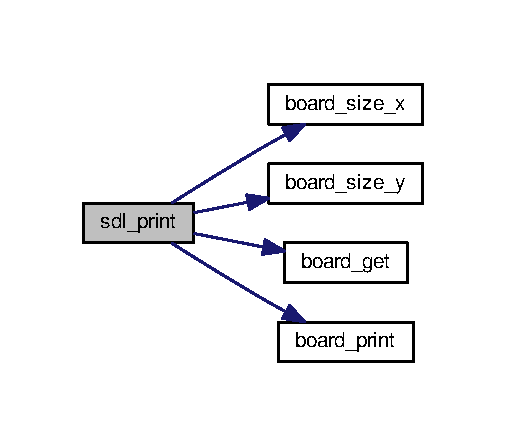
\includegraphics[width=243pt]{schlanga_8c_a2cfeae643e415db24e85db6c4994b071_cgraph}
\end{center}
\end{figure}




Voici le graphe des appelants de cette fonction \+:\nopagebreak
\begin{figure}[H]
\begin{center}
\leavevmode
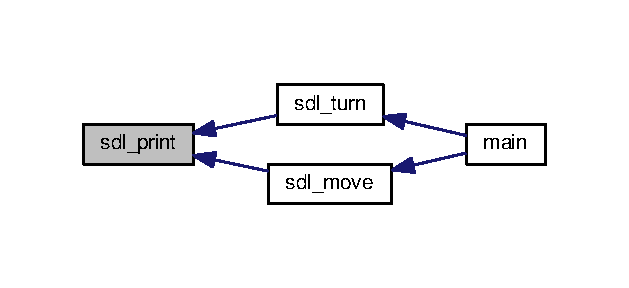
\includegraphics[width=302pt]{schlanga_8c_a2cfeae643e415db24e85db6c4994b071_icgraph}
\end{center}
\end{figure}


\index{schlanga.\+c@{schlanga.\+c}!sdl\+\_\+turn@{sdl\+\_\+turn}}
\index{sdl\+\_\+turn@{sdl\+\_\+turn}!schlanga.\+c@{schlanga.\+c}}
\subsubsection[{\texorpdfstring{sdl\+\_\+turn()}{sdl_turn()}}]{\setlength{\rightskip}{0pt plus 5cm}void$\ast$ sdl\+\_\+turn (
\begin{DoxyParamCaption}
{}
\end{DoxyParamCaption}
)}\hypertarget{schlanga_8c_ab6f22cbb52dc4a7603d7c42a3521a7c6}{}\label{schlanga_8c_ab6f22cbb52dc4a7603d7c42a3521a7c6}

\begin{DoxyCode}
80 \{
81     SDL\_Event event;
82     \textcolor{keywordflow}{while} (\hyperlink{schlanga_8c_aab1bde286e010d81472b269b419806d6}{X}) 
83     \{
84     SDL\_WaitEvent(&event);
85         \textcolor{keywordflow}{switch} (event.type) 
86         \{
87             \textcolor{keywordflow}{case} SDL\_QUIT:
88                 \hyperlink{schlanga_8c_aab1bde286e010d81472b269b419806d6}{X} = \textcolor{keyword}{false};
89                 \textcolor{keywordflow}{break};
90             \textcolor{keywordflow}{case} SDL\_KEYDOWN:
91                 \textcolor{keywordflow}{switch} (event.key.keysym.sym) 
92                 \{
93                     \textcolor{keywordflow}{case} SDLK\_ESCAPE:
94                         \hyperlink{schlanga_8c_aab1bde286e010d81472b269b419806d6}{X} = \textcolor{keyword}{false};
95                         \textcolor{keywordflow}{break};
96                     \textcolor{keywordflow}{case} SDLK\_RIGHT:\textcolor{comment}{/* key right */}
97                     \textcolor{keywordflow}{case} SDLK\_KP3:\textcolor{comment}{/* keypad 3 */}
98                     \textcolor{keywordflow}{case} SDLK\_KP9:\textcolor{comment}{/* keypad 3 */}
99                     \textcolor{keywordflow}{case} \textcolor{charliteral}{'e'}:\textcolor{comment}{/* code ascii */}
100                         \textcolor{comment}{/* on ferme la variable mutex */}
101                         pthread\_mutex\_lock(&\hyperlink{schlanga_8c_a4acff8232e4aec9cd5c6dc200ac55ef3}{mutex});
102                         \textcolor{comment}{/* turn snake */}
103                         \hyperlink{snakelib_8c_afa428ecb4385e08a82520bec11bafe36}{turn}(&\hyperlink{schlanga_8c_a20fdbd342281b7b5b77945c79d176b9f}{b},&\hyperlink{schlanga_8c_a71e92e96b65208605aca57598cc827f1}{s},1,\textcolor{charliteral}{'@'});
104                         \hyperlink{schlangalib_8c_a28adbac02fbdf8816543c25878bfd81d}{schlanga\_ia}(&\hyperlink{schlanga_8c_a20fdbd342281b7b5b77945c79d176b9f}{b},&\hyperlink{schlanga_8c_a71e92e96b65208605aca57598cc827f1}{s},&\hyperlink{schlanga_8c_aa6fd7c53c9b79f5a6ccb6f73b383263c}{c},\hyperlink{schlanga_8c_a37a78e9845fe459f5a2be9fe6ce52d24}{SNAKE\_LEN});
105                         \textcolor{keywordflow}{if} ((\hyperlink{schlanga_8c_aab1bde286e010d81472b269b419806d6}{X} = !(\hyperlink{snakelib_8c_ab96735ae82693727289ffe22fc940235}{choc\_snake}(&\hyperlink{schlanga_8c_a71e92e96b65208605aca57598cc827f1}{s},&\hyperlink{schlanga_8c_a71e92e96b65208605aca57598cc827f1}{s}))\(\backslash\)
106                             && !(\hyperlink{snakelib_8c_a50fa8a047abfa006a3371a94809e72c4}{choc\_wall}(&\hyperlink{schlanga_8c_a20fdbd342281b7b5b77945c79d176b9f}{b},&\hyperlink{schlanga_8c_a71e92e96b65208605aca57598cc827f1}{s}))\(\backslash\)
107                             && !(\hyperlink{snakelib_8c_ab96735ae82693727289ffe22fc940235}{choc\_snake}(&\hyperlink{schlanga_8c_aa6fd7c53c9b79f5a6ccb6f73b383263c}{c},&\hyperlink{schlanga_8c_aa6fd7c53c9b79f5a6ccb6f73b383263c}{c}))\(\backslash\)
108                             && !(\hyperlink{snakelib_8c_a50fa8a047abfa006a3371a94809e72c4}{choc\_wall}(&\hyperlink{schlanga_8c_a20fdbd342281b7b5b77945c79d176b9f}{b},&\hyperlink{schlanga_8c_aa6fd7c53c9b79f5a6ccb6f73b383263c}{c}))\(\backslash\)
109                             && !(\hyperlink{snakelib_8c_ab96735ae82693727289ffe22fc940235}{choc\_snake}(&\hyperlink{schlanga_8c_aa6fd7c53c9b79f5a6ccb6f73b383263c}{c},&\hyperlink{schlanga_8c_a71e92e96b65208605aca57598cc827f1}{s}))\(\backslash\)
110                             && !(\hyperlink{snakelib_8c_ab96735ae82693727289ffe22fc940235}{choc\_snake}(&\hyperlink{schlanga_8c_a71e92e96b65208605aca57598cc827f1}{s},&\hyperlink{schlanga_8c_aa6fd7c53c9b79f5a6ccb6f73b383263c}{c}))))
111                         
112                         \{
113                             \hyperlink{schlanga_8c_a2cfeae643e415db24e85db6c4994b071}{sdl\_print}();
114                         \}
115                         pthread\_mutex\_unlock(&\hyperlink{schlanga_8c_a4acff8232e4aec9cd5c6dc200ac55ef3}{mutex});
116                         \textcolor{keywordflow}{break};
117                     \textcolor{keywordflow}{case} SDLK\_LEFT:\textcolor{comment}{/* key left */}
118                     \textcolor{keywordflow}{case} SDLK\_KP1:\textcolor{comment}{/* keypad 1*/}
119                     \textcolor{keywordflow}{case} SDLK\_KP7:\textcolor{comment}{/* keypad 7*/}
120                     \textcolor{keywordflow}{case} \textcolor{charliteral}{'a'}:\textcolor{comment}{/* code ascii */}
121                         \textcolor{comment}{/* on ferme la variable mutex */}
122                         pthread\_mutex\_lock(&\hyperlink{schlanga_8c_a4acff8232e4aec9cd5c6dc200ac55ef3}{mutex});
123                         \textcolor{comment}{/* turn snake */}
124                         \hyperlink{snakelib_8c_afa428ecb4385e08a82520bec11bafe36}{turn}(&\hyperlink{schlanga_8c_a20fdbd342281b7b5b77945c79d176b9f}{b},&\hyperlink{schlanga_8c_a71e92e96b65208605aca57598cc827f1}{s},-1,\textcolor{charliteral}{'@'});
125                         \hyperlink{schlangalib_8c_a28adbac02fbdf8816543c25878bfd81d}{schlanga\_ia}(&\hyperlink{schlanga_8c_a20fdbd342281b7b5b77945c79d176b9f}{b},&\hyperlink{schlanga_8c_a71e92e96b65208605aca57598cc827f1}{s},&\hyperlink{schlanga_8c_aa6fd7c53c9b79f5a6ccb6f73b383263c}{c},\hyperlink{schlanga_8c_a37a78e9845fe459f5a2be9fe6ce52d24}{SNAKE\_LEN});
126                         \textcolor{keywordflow}{if} ((\hyperlink{schlanga_8c_aab1bde286e010d81472b269b419806d6}{X} = !(\hyperlink{snakelib_8c_ab96735ae82693727289ffe22fc940235}{choc\_snake}(&\hyperlink{schlanga_8c_a71e92e96b65208605aca57598cc827f1}{s},&\hyperlink{schlanga_8c_a71e92e96b65208605aca57598cc827f1}{s}))\(\backslash\)
127                             && !(\hyperlink{snakelib_8c_a50fa8a047abfa006a3371a94809e72c4}{choc\_wall}(&\hyperlink{schlanga_8c_a20fdbd342281b7b5b77945c79d176b9f}{b},&\hyperlink{schlanga_8c_a71e92e96b65208605aca57598cc827f1}{s}))\(\backslash\)
128                             && !(\hyperlink{snakelib_8c_ab96735ae82693727289ffe22fc940235}{choc\_snake}(&\hyperlink{schlanga_8c_aa6fd7c53c9b79f5a6ccb6f73b383263c}{c},&\hyperlink{schlanga_8c_aa6fd7c53c9b79f5a6ccb6f73b383263c}{c}))\(\backslash\)
129                             && !(\hyperlink{snakelib_8c_a50fa8a047abfa006a3371a94809e72c4}{choc\_wall}(&\hyperlink{schlanga_8c_a20fdbd342281b7b5b77945c79d176b9f}{b},&\hyperlink{schlanga_8c_aa6fd7c53c9b79f5a6ccb6f73b383263c}{c}))\(\backslash\)
130                             && !(\hyperlink{snakelib_8c_ab96735ae82693727289ffe22fc940235}{choc\_snake}(&\hyperlink{schlanga_8c_aa6fd7c53c9b79f5a6ccb6f73b383263c}{c},&\hyperlink{schlanga_8c_a71e92e96b65208605aca57598cc827f1}{s}))\(\backslash\)
131                             && !(\hyperlink{snakelib_8c_ab96735ae82693727289ffe22fc940235}{choc\_snake}(&\hyperlink{schlanga_8c_a71e92e96b65208605aca57598cc827f1}{s},&\hyperlink{schlanga_8c_aa6fd7c53c9b79f5a6ccb6f73b383263c}{c}))))
132                         \{
133                             \hyperlink{schlanga_8c_a2cfeae643e415db24e85db6c4994b071}{sdl\_print}();
134                         \}
135                         pthread\_mutex\_unlock(&\hyperlink{schlanga_8c_a4acff8232e4aec9cd5c6dc200ac55ef3}{mutex});
136                         \textcolor{keywordflow}{break};
137                     \textcolor{keywordflow}{default}:\textcolor{comment}{/* ne fait rien */}\textcolor{keywordflow}{break};
138                 \}   
139             \textcolor{keywordflow}{default}:\textcolor{comment}{/* ne fait rien */}\textcolor{keywordflow}{break};
140         \}
141     \}
142     pthread\_exit(0);
143 \}
\end{DoxyCode}


Voici le graphe d\textquotesingle{}appel pour cette fonction \+:\nopagebreak
\begin{figure}[H]
\begin{center}
\leavevmode
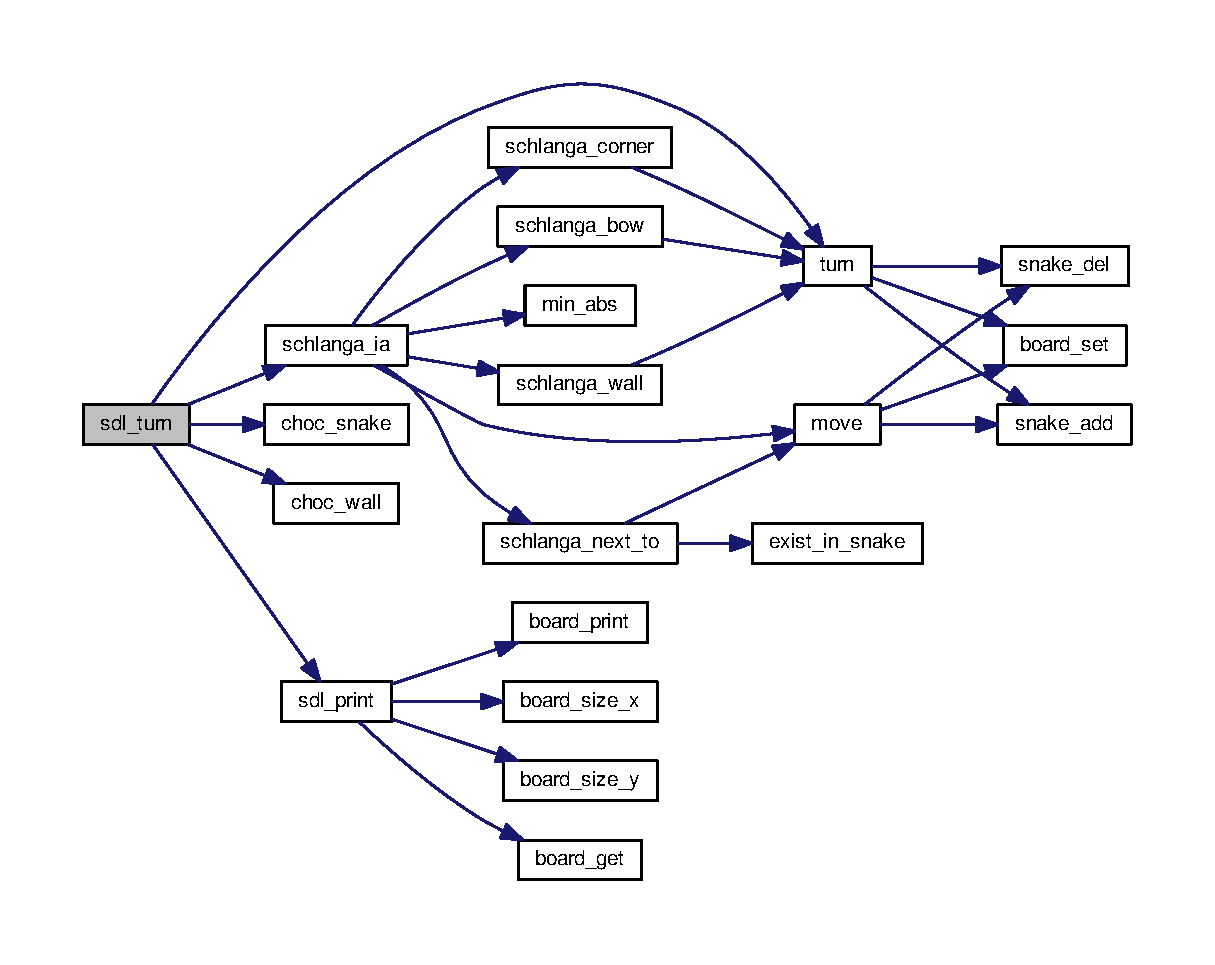
\includegraphics[width=350pt]{schlanga_8c_ab6f22cbb52dc4a7603d7c42a3521a7c6_cgraph}
\end{center}
\end{figure}




Voici le graphe des appelants de cette fonction \+:\nopagebreak
\begin{figure}[H]
\begin{center}
\leavevmode
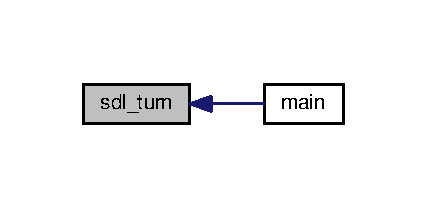
\includegraphics[width=205pt]{schlanga_8c_ab6f22cbb52dc4a7603d7c42a3521a7c6_icgraph}
\end{center}
\end{figure}




\subsection{Documentation des variables}
\index{schlanga.\+c@{schlanga.\+c}!A@{A}}
\index{A@{A}!schlanga.\+c@{schlanga.\+c}}
\subsubsection[{\texorpdfstring{A}{A}}]{\setlength{\rightskip}{0pt plus 5cm}S\+D\+L\+\_\+\+Surface $\ast$ A}\hypertarget{schlanga_8c_a79a54bef7bf02b18264c38fc90549a04}{}\label{schlanga_8c_a79a54bef7bf02b18264c38fc90549a04}
\index{schlanga.\+c@{schlanga.\+c}!B@{B}}
\index{B@{B}!schlanga.\+c@{schlanga.\+c}}
\subsubsection[{\texorpdfstring{B}{B}}]{\setlength{\rightskip}{0pt plus 5cm}S\+D\+L\+\_\+\+Surface $\ast$ B}\hypertarget{schlanga_8c_ac54b5255531a4799123d0f8dca96a7cc}{}\label{schlanga_8c_ac54b5255531a4799123d0f8dca96a7cc}
\index{schlanga.\+c@{schlanga.\+c}!b@{b}}
\index{b@{b}!schlanga.\+c@{schlanga.\+c}}
\subsubsection[{\texorpdfstring{b}{b}}]{\setlength{\rightskip}{0pt plus 5cm}{\bf board} b}\hypertarget{schlanga_8c_a20fdbd342281b7b5b77945c79d176b9f}{}\label{schlanga_8c_a20fdbd342281b7b5b77945c79d176b9f}
\index{schlanga.\+c@{schlanga.\+c}!C@{C}}
\index{C@{C}!schlanga.\+c@{schlanga.\+c}}
\subsubsection[{\texorpdfstring{C}{C}}]{\setlength{\rightskip}{0pt plus 5cm}S\+D\+L\+\_\+\+Surface $\ast$ C}\hypertarget{schlanga_8c_ab7d76262118cf1d4da44315136e542ca}{}\label{schlanga_8c_ab7d76262118cf1d4da44315136e542ca}
\index{schlanga.\+c@{schlanga.\+c}!c@{c}}
\index{c@{c}!schlanga.\+c@{schlanga.\+c}}
\subsubsection[{\texorpdfstring{c}{c}}]{\setlength{\rightskip}{0pt plus 5cm}{\bf snake} c}\hypertarget{schlanga_8c_aa6fd7c53c9b79f5a6ccb6f73b383263c}{}\label{schlanga_8c_aa6fd7c53c9b79f5a6ccb6f73b383263c}
\index{schlanga.\+c@{schlanga.\+c}!D@{D}}
\index{D@{D}!schlanga.\+c@{schlanga.\+c}}
\subsubsection[{\texorpdfstring{D}{D}}]{\setlength{\rightskip}{0pt plus 5cm}S\+D\+L\+\_\+\+Surface $\ast$ D}\hypertarget{schlanga_8c_aae9bd8b56defc5a6ec9c20b503b59a3a}{}\label{schlanga_8c_aae9bd8b56defc5a6ec9c20b503b59a3a}
\index{schlanga.\+c@{schlanga.\+c}!E@{E}}
\index{E@{E}!schlanga.\+c@{schlanga.\+c}}
\subsubsection[{\texorpdfstring{E}{E}}]{\setlength{\rightskip}{0pt plus 5cm}S\+D\+L\+\_\+\+Surface$\ast$ E}\hypertarget{schlanga_8c_ae8dfea36e66ed4b47c61a7ea5212e164}{}\label{schlanga_8c_ae8dfea36e66ed4b47c61a7ea5212e164}
\index{schlanga.\+c@{schlanga.\+c}!mutex@{mutex}}
\index{mutex@{mutex}!schlanga.\+c@{schlanga.\+c}}
\subsubsection[{\texorpdfstring{mutex}{mutex}}]{\setlength{\rightskip}{0pt plus 5cm}pthread\+\_\+mutex\+\_\+t mutex = P\+T\+H\+R\+E\+A\+D\+\_\+\+M\+U\+T\+E\+X\+\_\+\+I\+N\+I\+T\+I\+A\+L\+I\+Z\+ER}\hypertarget{schlanga_8c_a4acff8232e4aec9cd5c6dc200ac55ef3}{}\label{schlanga_8c_a4acff8232e4aec9cd5c6dc200ac55ef3}
\index{schlanga.\+c@{schlanga.\+c}!s@{s}}
\index{s@{s}!schlanga.\+c@{schlanga.\+c}}
\subsubsection[{\texorpdfstring{s}{s}}]{\setlength{\rightskip}{0pt plus 5cm}{\bf snake} s}\hypertarget{schlanga_8c_a71e92e96b65208605aca57598cc827f1}{}\label{schlanga_8c_a71e92e96b65208605aca57598cc827f1}
\index{schlanga.\+c@{schlanga.\+c}!X@{X}}
\index{X@{X}!schlanga.\+c@{schlanga.\+c}}
\subsubsection[{\texorpdfstring{X}{X}}]{\setlength{\rightskip}{0pt plus 5cm}bool X}\hypertarget{schlanga_8c_aab1bde286e010d81472b269b419806d6}{}\label{schlanga_8c_aab1bde286e010d81472b269b419806d6}

\hypertarget{schlangalib_8c}{}\section{Référence du fichier S\+O\+U\+R\+C\+E/schlangalib.c}
\label{schlangalib_8c}\index{S\+O\+U\+R\+C\+E/schlangalib.\+c@{S\+O\+U\+R\+C\+E/schlangalib.\+c}}
{\ttfamily \#include $<$stdlib.\+h$>$}\\*
{\ttfamily \#include $<$stdbool.\+h$>$}\\*
{\ttfamily \#include \char`\"{}../\+I\+N\+C\+L\+U\+D\+E/snakelib.\+h\char`\"{}}\\*
{\ttfamily \#include \char`\"{}../\+I\+N\+C\+L\+U\+D\+E/schlangalib.\+h\char`\"{}}\\*
Graphe des dépendances par inclusion de schlangalib.\+c\+:\nopagebreak
\begin{figure}[H]
\begin{center}
\leavevmode
\includegraphics[width=350pt]{schlangalib_8c__incl}
\end{center}
\end{figure}
\subsection*{Macros}
\begin{DoxyCompactItemize}
\item 
\#define \hyperlink{schlangalib_8c_a012777a0d47b27fcae56ae35614459dd}{C\+O\+D\+E\+\_\+\+N\+U\+LL}~0
\item 
\#define \hyperlink{schlangalib_8c_aea2ff5b1ef8a3b2b9a385927575c9396}{C\+O\+D\+E\+\_\+\+B\+OW}~1
\item 
\#define \hyperlink{schlangalib_8c_acee163547d72d28d7cbb45de2c1cc1b9}{C\+O\+D\+E\+\_\+\+W\+A\+LL}~2
\item 
\#define \hyperlink{schlangalib_8c_a91640b78c7bda96c44c256a09f02e700}{C\+O\+D\+E\+\_\+\+C\+O\+R\+N\+ER}~3
\item 
\#define \hyperlink{schlangalib_8c_a4baca3e22ae44aafc8a52b0768491cd3}{C\+O\+D\+E\+\_\+\+N\+E\+X\+T\+\_\+\+TO}~4
\end{DoxyCompactItemize}
\subsection*{Fonctions}
\begin{DoxyCompactItemize}
\item 
bool \hyperlink{schlangalib_8c_a6c97e3271fe6b65bd31bdbaf03bf6b9c}{exist\+\_\+in\+\_\+snake} (const \hyperlink{structsnake}{snake} $\ast$\hyperlink{snake_8c_a71e92e96b65208605aca57598cc827f1}{s}, int x, int y)
\item 
bool \hyperlink{schlangalib_8c_a4cb830baa18247d13d465075c869d1d7}{schlanga\+\_\+bow} (\hyperlink{structboard}{board} $\ast$\hyperlink{snake_8c_a20fdbd342281b7b5b77945c79d176b9f}{b}, const \hyperlink{structsnake}{snake} $\ast$\hyperlink{snake_8c_a71e92e96b65208605aca57598cc827f1}{s}, \hyperlink{structsnake}{snake} $\ast$\hyperlink{schlanga_8c_aa6fd7c53c9b79f5a6ccb6f73b383263c}{c})
\item 
bool \hyperlink{schlangalib_8c_a5b8413626002409e9465985272966386}{schlanga\+\_\+wall} (\hyperlink{structboard}{board} $\ast$\hyperlink{snake_8c_a20fdbd342281b7b5b77945c79d176b9f}{b}, \hyperlink{structsnake}{snake} $\ast$\hyperlink{schlanga_8c_aa6fd7c53c9b79f5a6ccb6f73b383263c}{c})
\item 
bool \hyperlink{schlangalib_8c_a08f1c27d2a4dd425ca550057e8856240}{schlanga\+\_\+corner} (\hyperlink{structboard}{board} $\ast$\hyperlink{snake_8c_a20fdbd342281b7b5b77945c79d176b9f}{b}, \hyperlink{structsnake}{snake} $\ast$\hyperlink{schlanga_8c_aa6fd7c53c9b79f5a6ccb6f73b383263c}{c})
\item 
bool \hyperlink{schlangalib_8c_a2655a50383ab9680d1a3a72ea9de562d}{schlanga\+\_\+next\+\_\+to} (\hyperlink{structboard}{board} $\ast$\hyperlink{snake_8c_a20fdbd342281b7b5b77945c79d176b9f}{b}, const \hyperlink{structsnake}{snake} $\ast$\hyperlink{snake_8c_a71e92e96b65208605aca57598cc827f1}{s}, \hyperlink{structsnake}{snake} $\ast$\hyperlink{schlanga_8c_aa6fd7c53c9b79f5a6ccb6f73b383263c}{c})
\item 
int \hyperlink{schlangalib_8c_af3fdd05c8d6e18536c1f89f1814969d4}{min\+\_\+abs} (int a, int \hyperlink{snake_8c_a20fdbd342281b7b5b77945c79d176b9f}{b})
\item 
void \hyperlink{schlangalib_8c_a28adbac02fbdf8816543c25878bfd81d}{schlanga\+\_\+ia} (\hyperlink{structboard}{board} $\ast$\hyperlink{snake_8c_a20fdbd342281b7b5b77945c79d176b9f}{b}, const \hyperlink{structsnake}{snake} $\ast$\hyperlink{snake_8c_a71e92e96b65208605aca57598cc827f1}{s}, \hyperlink{structsnake}{snake} $\ast$\hyperlink{schlanga_8c_aa6fd7c53c9b79f5a6ccb6f73b383263c}{c}, int len)
\end{DoxyCompactItemize}


\subsection{Documentation des macros}
\index{schlangalib.\+c@{schlangalib.\+c}!C\+O\+D\+E\+\_\+\+B\+OW@{C\+O\+D\+E\+\_\+\+B\+OW}}
\index{C\+O\+D\+E\+\_\+\+B\+OW@{C\+O\+D\+E\+\_\+\+B\+OW}!schlangalib.\+c@{schlangalib.\+c}}
\subsubsection[{\texorpdfstring{C\+O\+D\+E\+\_\+\+B\+OW}{CODE_BOW}}]{\setlength{\rightskip}{0pt plus 5cm}\#define C\+O\+D\+E\+\_\+\+B\+OW~1}\hypertarget{schlangalib_8c_aea2ff5b1ef8a3b2b9a385927575c9396}{}\label{schlangalib_8c_aea2ff5b1ef8a3b2b9a385927575c9396}
\index{schlangalib.\+c@{schlangalib.\+c}!C\+O\+D\+E\+\_\+\+C\+O\+R\+N\+ER@{C\+O\+D\+E\+\_\+\+C\+O\+R\+N\+ER}}
\index{C\+O\+D\+E\+\_\+\+C\+O\+R\+N\+ER@{C\+O\+D\+E\+\_\+\+C\+O\+R\+N\+ER}!schlangalib.\+c@{schlangalib.\+c}}
\subsubsection[{\texorpdfstring{C\+O\+D\+E\+\_\+\+C\+O\+R\+N\+ER}{CODE_CORNER}}]{\setlength{\rightskip}{0pt plus 5cm}\#define C\+O\+D\+E\+\_\+\+C\+O\+R\+N\+ER~3}\hypertarget{schlangalib_8c_a91640b78c7bda96c44c256a09f02e700}{}\label{schlangalib_8c_a91640b78c7bda96c44c256a09f02e700}
\index{schlangalib.\+c@{schlangalib.\+c}!C\+O\+D\+E\+\_\+\+N\+E\+X\+T\+\_\+\+TO@{C\+O\+D\+E\+\_\+\+N\+E\+X\+T\+\_\+\+TO}}
\index{C\+O\+D\+E\+\_\+\+N\+E\+X\+T\+\_\+\+TO@{C\+O\+D\+E\+\_\+\+N\+E\+X\+T\+\_\+\+TO}!schlangalib.\+c@{schlangalib.\+c}}
\subsubsection[{\texorpdfstring{C\+O\+D\+E\+\_\+\+N\+E\+X\+T\+\_\+\+TO}{CODE_NEXT_TO}}]{\setlength{\rightskip}{0pt plus 5cm}\#define C\+O\+D\+E\+\_\+\+N\+E\+X\+T\+\_\+\+TO~4}\hypertarget{schlangalib_8c_a4baca3e22ae44aafc8a52b0768491cd3}{}\label{schlangalib_8c_a4baca3e22ae44aafc8a52b0768491cd3}
\index{schlangalib.\+c@{schlangalib.\+c}!C\+O\+D\+E\+\_\+\+N\+U\+LL@{C\+O\+D\+E\+\_\+\+N\+U\+LL}}
\index{C\+O\+D\+E\+\_\+\+N\+U\+LL@{C\+O\+D\+E\+\_\+\+N\+U\+LL}!schlangalib.\+c@{schlangalib.\+c}}
\subsubsection[{\texorpdfstring{C\+O\+D\+E\+\_\+\+N\+U\+LL}{CODE_NULL}}]{\setlength{\rightskip}{0pt plus 5cm}\#define C\+O\+D\+E\+\_\+\+N\+U\+LL~0}\hypertarget{schlangalib_8c_a012777a0d47b27fcae56ae35614459dd}{}\label{schlangalib_8c_a012777a0d47b27fcae56ae35614459dd}
\index{schlangalib.\+c@{schlangalib.\+c}!C\+O\+D\+E\+\_\+\+W\+A\+LL@{C\+O\+D\+E\+\_\+\+W\+A\+LL}}
\index{C\+O\+D\+E\+\_\+\+W\+A\+LL@{C\+O\+D\+E\+\_\+\+W\+A\+LL}!schlangalib.\+c@{schlangalib.\+c}}
\subsubsection[{\texorpdfstring{C\+O\+D\+E\+\_\+\+W\+A\+LL}{CODE_WALL}}]{\setlength{\rightskip}{0pt plus 5cm}\#define C\+O\+D\+E\+\_\+\+W\+A\+LL~2}\hypertarget{schlangalib_8c_acee163547d72d28d7cbb45de2c1cc1b9}{}\label{schlangalib_8c_acee163547d72d28d7cbb45de2c1cc1b9}


\subsection{Documentation des fonctions}
\index{schlangalib.\+c@{schlangalib.\+c}!exist\+\_\+in\+\_\+snake@{exist\+\_\+in\+\_\+snake}}
\index{exist\+\_\+in\+\_\+snake@{exist\+\_\+in\+\_\+snake}!schlangalib.\+c@{schlangalib.\+c}}
\subsubsection[{\texorpdfstring{exist\+\_\+in\+\_\+snake(const snake $\ast$s, int x, int y)}{exist_in_snake(const snake *s, int x, int y)}}]{\setlength{\rightskip}{0pt plus 5cm}bool exist\+\_\+in\+\_\+snake (
\begin{DoxyParamCaption}
\item[{const {\bf snake} $\ast$}]{s, }
\item[{int}]{x, }
\item[{int}]{y}
\end{DoxyParamCaption}
)}\hypertarget{schlangalib_8c_a6c97e3271fe6b65bd31bdbaf03bf6b9c}{}\label{schlangalib_8c_a6c97e3271fe6b65bd31bdbaf03bf6b9c}

\begin{DoxyCode}
21 \{
22     \hyperlink{structsnake}{snake} curr = *\hyperlink{client_8c_a71e92e96b65208605aca57598cc827f1}{s};
23     \textcolor{keywordflow}{while}(curr != 0)
24     \{
25         \textcolor{keywordflow}{if}(curr->x == x && curr->y == y)
26         \{
27             \textcolor{keywordflow}{return} \textcolor{keyword}{true};
28         \}
29         curr = curr->next;
30     \}
31     \textcolor{keywordflow}{return} \textcolor{keyword}{false};
32 \}
\end{DoxyCode}


Voici le graphe des appelants de cette fonction \+:\nopagebreak
\begin{figure}[H]
\begin{center}
\leavevmode
\includegraphics[width=350pt]{schlangalib_8c_a6c97e3271fe6b65bd31bdbaf03bf6b9c_icgraph}
\end{center}
\end{figure}


\index{schlangalib.\+c@{schlangalib.\+c}!min\+\_\+abs@{min\+\_\+abs}}
\index{min\+\_\+abs@{min\+\_\+abs}!schlangalib.\+c@{schlangalib.\+c}}
\subsubsection[{\texorpdfstring{min\+\_\+abs(int a, int b)}{min_abs(int a, int b)}}]{\setlength{\rightskip}{0pt plus 5cm}int min\+\_\+abs (
\begin{DoxyParamCaption}
\item[{int}]{a, }
\item[{int}]{b}
\end{DoxyParamCaption}
)}\hypertarget{schlangalib_8c_af3fdd05c8d6e18536c1f89f1814969d4}{}\label{schlangalib_8c_af3fdd05c8d6e18536c1f89f1814969d4}

\begin{DoxyCode}
421 \{
422     \textcolor{keywordflow}{if}(a < 0)
423         a = -a;
424     \textcolor{keywordflow}{if}(\hyperlink{client_8c_a20fdbd342281b7b5b77945c79d176b9f}{b} < 0)
425         \hyperlink{client_8c_a20fdbd342281b7b5b77945c79d176b9f}{b} = -\hyperlink{client_8c_a20fdbd342281b7b5b77945c79d176b9f}{b};
426     \textcolor{keywordflow}{return} (a < \hyperlink{client_8c_a20fdbd342281b7b5b77945c79d176b9f}{b})? a : \hyperlink{client_8c_a20fdbd342281b7b5b77945c79d176b9f}{b};
427 \}
\end{DoxyCode}


Voici le graphe des appelants de cette fonction \+:\nopagebreak
\begin{figure}[H]
\begin{center}
\leavevmode
\includegraphics[width=350pt]{schlangalib_8c_af3fdd05c8d6e18536c1f89f1814969d4_icgraph}
\end{center}
\end{figure}


\index{schlangalib.\+c@{schlangalib.\+c}!schlanga\+\_\+bow@{schlanga\+\_\+bow}}
\index{schlanga\+\_\+bow@{schlanga\+\_\+bow}!schlangalib.\+c@{schlangalib.\+c}}
\subsubsection[{\texorpdfstring{schlanga\+\_\+bow(board $\ast$b, const snake $\ast$s, snake $\ast$c)}{schlanga_bow(board *b, const snake *s, snake *c)}}]{\setlength{\rightskip}{0pt plus 5cm}bool schlanga\+\_\+bow (
\begin{DoxyParamCaption}
\item[{{\bf board} $\ast$}]{b, }
\item[{const {\bf snake} $\ast$}]{s, }
\item[{{\bf snake} $\ast$}]{c}
\end{DoxyParamCaption}
)}\hypertarget{schlangalib_8c_a4cb830baa18247d13d465075c869d1d7}{}\label{schlangalib_8c_a4cb830baa18247d13d465075c869d1d7}

\begin{DoxyCode}
43 \{
44     \hyperlink{structsnake}{snake} curr = *\hyperlink{client_8c_a71e92e96b65208605aca57598cc827f1}{s};
45     \hyperlink{structsnake}{snake} head = *\hyperlink{client_8c_a71e92e96b65208605aca57598cc827f1}{s};
46     \textcolor{keywordtype}{bool} danger = \textcolor{keyword}{false};
47     \textcolor{keywordtype}{int} schla\_dir\_x = (*c)->x - (*c)->next->x;
48     \textcolor{keywordtype}{int} schla\_dir\_y = (*c)->y - (*c)->next->y;
49     \textcolor{keywordflow}{while}(curr != 0)
50     \{
51         \textcolor{keywordflow}{if}(\(\backslash\)
52             ((*c)->x + schla\_dir\_x == curr->x) && ((*c)->y == curr->y)\(\backslash\)
53         )
54         \{
55             danger = \textcolor{keyword}{true};
56             \textcolor{keywordflow}{break};
57         \}
58         \textcolor{keywordflow}{if}(\(\backslash\)
59             ((*c)->x + 2*schla\_dir\_x == curr->x) && ((*c)->y == curr->y)\(\backslash\)
60         )
61         \{
62             danger = \textcolor{keyword}{true};
63             \textcolor{keywordflow}{break};
64         \}
65         \textcolor{keywordflow}{if}(\(\backslash\)
66             ((*c)->x + 3*schla\_dir\_x == curr->x) && ((*c)->y == curr->y)\(\backslash\)
67         )
68         \{
69             danger = \textcolor{keyword}{true};
70             \textcolor{keywordflow}{break};
71         \}
72 
73 
74         \textcolor{keywordflow}{if}(\(\backslash\)
75             ((*c)->y + schla\_dir\_y == curr->y) && ((*c)->x == curr->x)\(\backslash\)
76         )
77         \{
78             danger = \textcolor{keyword}{true};
79             \textcolor{keywordflow}{break};
80         \}
81         \textcolor{keywordflow}{if}(\(\backslash\)
82             ((*c)->y + 2*schla\_dir\_y == curr->y) && ((*c)->x == curr->x)\(\backslash\)
83         )
84         \{
85             danger = \textcolor{keyword}{true};
86             \textcolor{keywordflow}{break};
87         \}
88         \textcolor{keywordflow}{if}(\(\backslash\)
89             ((*c)->y + 3*schla\_dir\_y == curr->y) && ((*c)->x == curr->x)\(\backslash\)
90         )
91         \{
92             danger = \textcolor{keyword}{true};
93             \textcolor{keywordflow}{break};
94         \}
95         curr = curr->next;
96     \}
97     \textcolor{keywordflow}{if}(danger)
98     \{
99         \textcolor{keywordtype}{int} snake\_dir\_x = head->x - head->next->x;
100         \textcolor{keywordtype}{int} snake\_dir\_y = head->y - head->next->y;
101         \textcolor{keywordtype}{int} snake\_bow\_x = 0, snake\_bow\_y = 0;
102         \textcolor{keywordtype}{int} dx = 0, dy = 0;
103         curr = *\hyperlink{client_8c_a71e92e96b65208605aca57598cc827f1}{s};
104         \textcolor{keywordflow}{while}(snake\_bow\_x == 0\(\backslash\)
105             && snake\_bow\_y == 0\(\backslash\)
106             && curr->next->next != 0)
107         \{
108             dx = curr->x - curr->next->next->x;
109             dy = curr->y - curr->next->next->y;
110             \textcolor{keywordflow}{if}(dx != 0 && dy != 0)
111             \{
112                 snake\_bow\_x = dx;
113                 snake\_bow\_y = dy;
114                 \textcolor{keywordflow}{break};
115             \}
116             curr = curr->next;
117         \}
118         \textcolor{keywordflow}{if}(snake\_bow\_x == 1\(\backslash\)
119             && snake\_bow\_y == 1)
120         \{
121             \textcolor{keywordflow}{if}(snake\_dir\_x == 1)
122             \{
123                 \hyperlink{snakelib_8c_afa428ecb4385e08a82520bec11bafe36}{turn}(b,c,-1,\textcolor{charliteral}{'&'});
124                 \textcolor{keywordflow}{return} \textcolor{keyword}{true};
125             \}
126             \textcolor{keywordflow}{if}(snake\_dir\_y == 1)
127             \{
128                 \hyperlink{snakelib_8c_afa428ecb4385e08a82520bec11bafe36}{turn}(b,c,1,\textcolor{charliteral}{'&'});
129                 \textcolor{keywordflow}{return} \textcolor{keyword}{true};
130             \}
131         \}
132         \textcolor{keywordflow}{if}(snake\_bow\_x == 1\(\backslash\)
133             && snake\_bow\_y == -1)
134         \{
135             \textcolor{keywordflow}{if}(snake\_dir\_x == 1)
136             \{
137                 \hyperlink{snakelib_8c_afa428ecb4385e08a82520bec11bafe36}{turn}(b,c,1,\textcolor{charliteral}{'&'});
138                 \textcolor{keywordflow}{return} \textcolor{keyword}{true};
139             \}
140             \textcolor{keywordflow}{if}(snake\_dir\_y == -1)
141             \{
142                 \hyperlink{snakelib_8c_afa428ecb4385e08a82520bec11bafe36}{turn}(b,c,-1,\textcolor{charliteral}{'&'});
143                 \textcolor{keywordflow}{return} \textcolor{keyword}{true};
144             \}   
145         \}
146         \textcolor{keywordflow}{if}(snake\_bow\_x == -1\(\backslash\)
147             && snake\_bow\_y == 1)
148         \{
149             \textcolor{keywordflow}{if}(snake\_dir\_x == -1)
150             \{
151                 \hyperlink{snakelib_8c_afa428ecb4385e08a82520bec11bafe36}{turn}(b,c,1,\textcolor{charliteral}{'&'});
152                 \textcolor{keywordflow}{return} \textcolor{keyword}{true};
153             \}
154             \textcolor{keywordflow}{if}(snake\_dir\_y == 1)
155             \{
156                 \hyperlink{snakelib_8c_afa428ecb4385e08a82520bec11bafe36}{turn}(b,c,-1,\textcolor{charliteral}{'&'});
157                 \textcolor{keywordflow}{return} \textcolor{keyword}{true};
158             \}
159         \}
160         \textcolor{keywordflow}{if}(snake\_bow\_x == -1\(\backslash\)
161             && snake\_bow\_y == -1)
162         \{
163             \textcolor{keywordflow}{if}(snake\_dir\_x == -1)
164             \{
165                 \hyperlink{snakelib_8c_afa428ecb4385e08a82520bec11bafe36}{turn}(b,c,-1,\textcolor{charliteral}{'&'});
166                 \textcolor{keywordflow}{return} \textcolor{keyword}{true};
167             \}
168             \textcolor{keywordflow}{if}(snake\_dir\_y == -1)
169             \{
170                 \hyperlink{snakelib_8c_afa428ecb4385e08a82520bec11bafe36}{turn}(b,c,1,\textcolor{charliteral}{'&'});
171                 \textcolor{keywordflow}{return} \textcolor{keyword}{true};
172             \}   
173         \}
174         \hyperlink{snakelib_8c_afa428ecb4385e08a82520bec11bafe36}{turn}(b,c,(rand() % 2) * 2 - 1,\textcolor{charliteral}{'&'});
175         \textcolor{keywordflow}{return} \textcolor{keyword}{true};
176     \}
177     \textcolor{keywordflow}{return} \textcolor{keyword}{false};
178 \}
\end{DoxyCode}


Voici le graphe d\textquotesingle{}appel pour cette fonction \+:\nopagebreak
\begin{figure}[H]
\begin{center}
\leavevmode
\includegraphics[width=328pt]{schlangalib_8c_a4cb830baa18247d13d465075c869d1d7_cgraph}
\end{center}
\end{figure}




Voici le graphe des appelants de cette fonction \+:\nopagebreak
\begin{figure}[H]
\begin{center}
\leavevmode
\includegraphics[width=350pt]{schlangalib_8c_a4cb830baa18247d13d465075c869d1d7_icgraph}
\end{center}
\end{figure}


\index{schlangalib.\+c@{schlangalib.\+c}!schlanga\+\_\+corner@{schlanga\+\_\+corner}}
\index{schlanga\+\_\+corner@{schlanga\+\_\+corner}!schlangalib.\+c@{schlangalib.\+c}}
\subsubsection[{\texorpdfstring{schlanga\+\_\+corner(board $\ast$b, snake $\ast$c)}{schlanga_corner(board *b, snake *c)}}]{\setlength{\rightskip}{0pt plus 5cm}bool schlanga\+\_\+corner (
\begin{DoxyParamCaption}
\item[{{\bf board} $\ast$}]{b, }
\item[{{\bf snake} $\ast$}]{c}
\end{DoxyParamCaption}
)}\hypertarget{schlangalib_8c_a08f1c27d2a4dd425ca550057e8856240}{}\label{schlangalib_8c_a08f1c27d2a4dd425ca550057e8856240}

\begin{DoxyCode}
288 \{
289     \textcolor{keywordtype}{int} x\_board = 1;
290     \textcolor{keywordtype}{int} y\_board = 1;
291 
292     \textcolor{keywordtype}{int} dx\_board = b->\hyperlink{structboard_a45ad83890aed4b92ef175f0eb13cd1f3}{x} - 2;
293     \textcolor{keywordtype}{int} dy\_board = b->\hyperlink{structboard_a0a1685edc20c5b97527ccd4027d5f8eb}{y} - 2;
294 
295     \hyperlink{structsnake}{snake} head = (*c);
296 
297     \textcolor{keywordtype}{int} schlanga\_dir\_x = head->x - head->next->x;
298     \textcolor{keywordtype}{int} schlanga\_dir\_y = head->y - head->next->y;
299 
300     \textcolor{keywordflow}{if}(x\_board == head->x && y\_board == head->y)
301     \{
302         \textcolor{keywordflow}{if}(schlanga\_dir\_x)
303         \{
304             \hyperlink{snakelib_8c_afa428ecb4385e08a82520bec11bafe36}{turn}(b,c,-1,\textcolor{charliteral}{'&'});
305         \}
306         \textcolor{keywordflow}{if}(schlanga\_dir\_y)
307         \{
308             \hyperlink{snakelib_8c_afa428ecb4385e08a82520bec11bafe36}{turn}(b,c,1,\textcolor{charliteral}{'&'});
309         \}
310         \textcolor{keywordflow}{return} \textcolor{keyword}{true};
311     \}
312     \textcolor{keywordflow}{if}(x\_board == head->x && dy\_board == head->y)
313     \{
314         \textcolor{keywordflow}{if}(schlanga\_dir\_x)
315         \{
316             \hyperlink{snakelib_8c_afa428ecb4385e08a82520bec11bafe36}{turn}(b,c,1,\textcolor{charliteral}{'&'});
317         \}
318         \textcolor{keywordflow}{if}(schlanga\_dir\_y)
319         \{
320             \hyperlink{snakelib_8c_afa428ecb4385e08a82520bec11bafe36}{turn}(b,c,-1,\textcolor{charliteral}{'&'});   
321         \}
322         \textcolor{keywordflow}{return} \textcolor{keyword}{true};
323     \}
324     \textcolor{keywordflow}{if}(dx\_board == head->x && y\_board == head->y)
325     \{
326         \textcolor{keywordflow}{if}(schlanga\_dir\_x)
327         \{
328             \hyperlink{snakelib_8c_afa428ecb4385e08a82520bec11bafe36}{turn}(b,c,1,\textcolor{charliteral}{'&'});
329         \}
330         \textcolor{keywordflow}{if}(schlanga\_dir\_y)
331         \{
332             \hyperlink{snakelib_8c_afa428ecb4385e08a82520bec11bafe36}{turn}(b,c,-1,\textcolor{charliteral}{'&'});
333         \}
334         \textcolor{keywordflow}{return} \textcolor{keyword}{true};
335     \}
336     \textcolor{keywordflow}{if}(dx\_board == head->x && dy\_board == head->y)
337     \{
338         \textcolor{keywordflow}{if}(schlanga\_dir\_x)
339         \{
340             \hyperlink{snakelib_8c_afa428ecb4385e08a82520bec11bafe36}{turn}(b,c,-1,\textcolor{charliteral}{'&'});
341         \}
342         \textcolor{keywordflow}{if}(schlanga\_dir\_y)
343         \{
344             \hyperlink{snakelib_8c_afa428ecb4385e08a82520bec11bafe36}{turn}(b,c,1,\textcolor{charliteral}{'&'});
345         \}
346         \textcolor{keywordflow}{return} \textcolor{keyword}{true};
347     \}
348     \textcolor{keywordflow}{return} \textcolor{keyword}{false};
349 \}
\end{DoxyCode}


Voici le graphe d\textquotesingle{}appel pour cette fonction \+:\nopagebreak
\begin{figure}[H]
\begin{center}
\leavevmode
\includegraphics[width=337pt]{schlangalib_8c_a08f1c27d2a4dd425ca550057e8856240_cgraph}
\end{center}
\end{figure}




Voici le graphe des appelants de cette fonction \+:\nopagebreak
\begin{figure}[H]
\begin{center}
\leavevmode
\includegraphics[width=350pt]{schlangalib_8c_a08f1c27d2a4dd425ca550057e8856240_icgraph}
\end{center}
\end{figure}


\index{schlangalib.\+c@{schlangalib.\+c}!schlanga\+\_\+ia@{schlanga\+\_\+ia}}
\index{schlanga\+\_\+ia@{schlanga\+\_\+ia}!schlangalib.\+c@{schlangalib.\+c}}
\subsubsection[{\texorpdfstring{schlanga\+\_\+ia(board $\ast$b, const snake $\ast$s, snake $\ast$c, int len)}{schlanga_ia(board *b, const snake *s, snake *c, int len)}}]{\setlength{\rightskip}{0pt plus 5cm}void schlanga\+\_\+ia (
\begin{DoxyParamCaption}
\item[{{\bf board} $\ast$}]{b, }
\item[{const {\bf snake} $\ast$}]{s, }
\item[{{\bf snake} $\ast$}]{c, }
\item[{int}]{len}
\end{DoxyParamCaption}
)}\hypertarget{schlangalib_8c_a28adbac02fbdf8816543c25878bfd81d}{}\label{schlangalib_8c_a28adbac02fbdf8816543c25878bfd81d}

\begin{DoxyCode}
437 \{
438     \textcolor{keyword}{static} \textcolor{keywordtype}{int} code = \hyperlink{schlangalib_8c_a012777a0d47b27fcae56ae35614459dd}{CODE\_NULL};
439     \textcolor{keyword}{static} \textcolor{keywordtype}{int} count = 0;
440     \textcolor{keyword}{static} \textcolor{keywordtype}{int} corner = 0;
441     \textcolor{keywordtype}{int} x\_board = 1;
442     \textcolor{keywordtype}{int} y\_board = 1;
443 
444     \textcolor{keywordtype}{int} dx\_board = b->\hyperlink{structboard_a45ad83890aed4b92ef175f0eb13cd1f3}{x} - 2;
445     \textcolor{keywordtype}{int} dy\_board = b->\hyperlink{structboard_a0a1685edc20c5b97527ccd4027d5f8eb}{y} - 2;
446 
447     \textcolor{keywordtype}{int} schlanga\_x = (*c)->x;
448     \textcolor{keywordtype}{int} schlanga\_y = (*c)->y;
449 
450     \textcolor{keywordtype}{int} schlanga\_dir\_x = (*c)->x - (*c)->next->x;
451     \textcolor{keywordtype}{int} schlanga\_dir\_y = (*c)->y - (*c)->next->y;
452 
453     \textcolor{keywordflow}{if}(\hyperlink{schlangalib_8c_a2655a50383ab9680d1a3a72ea9de562d}{schlanga\_next\_to}(b,s,c))
454     \{
455         code = \hyperlink{schlangalib_8c_a4baca3e22ae44aafc8a52b0768491cd3}{CODE\_NEXT\_TO};
456         \textcolor{keywordflow}{return};
457     \}
458     \textcolor{keywordflow}{if}(\hyperlink{schlangalib_8c_a08f1c27d2a4dd425ca550057e8856240}{schlanga\_corner}(b,c))
459     \{
460         code = \hyperlink{schlangalib_8c_a91640b78c7bda96c44c256a09f02e700}{CODE\_CORNER};
461         corner = len/2-2;
462         \textcolor{keywordflow}{return};
463     \}
464     \textcolor{keywordflow}{if}(corner)
465     \{
466         \textcolor{keywordflow}{if}(\hyperlink{schlangalib_8c_a4cb830baa18247d13d465075c869d1d7}{schlanga\_bow}(b,s,c))
467         \{
468             corner = 0;
469             code = \hyperlink{schlangalib_8c_aea2ff5b1ef8a3b2b9a385927575c9396}{CODE\_BOW};
470         \}
471         \textcolor{keywordflow}{else}
472         \{
473             \hyperlink{snakelib_8c_aa7c9d4fed2b3edb453a4501ba019dc00}{move}(b,c,\textcolor{charliteral}{'&'});
474             --corner;
475         \}
476         \textcolor{keywordflow}{return};
477     \}
478     \textcolor{keywordflow}{if}(code != \hyperlink{schlangalib_8c_acee163547d72d28d7cbb45de2c1cc1b9}{CODE\_WALL})
479     \{
480         \textcolor{keywordflow}{if}(\hyperlink{schlangalib_8c_a5b8413626002409e9465985272966386}{schlanga\_wall}(b,c))
481         \{
482             code = \hyperlink{schlangalib_8c_acee163547d72d28d7cbb45de2c1cc1b9}{CODE\_WALL};
483             \textcolor{keywordtype}{unsigned} \hyperlink{client_8c_a67668278838ab1eb0065ef9218c8de00}{m} = 0;
484             \textcolor{keywordflow}{if}(schlanga\_dir\_x == 0)
485             \{
486                 m = \hyperlink{schlangalib_8c_af3fdd05c8d6e18536c1f89f1814969d4}{min\_abs}(schlanga\_x - x\_board, schlanga\_x - dx\_board);
487             \}
488             \textcolor{keywordflow}{if}(schlanga\_dir\_y == 0)
489             \{
490                 m = \hyperlink{schlangalib_8c_af3fdd05c8d6e18536c1f89f1814969d4}{min\_abs}(schlanga\_y - y\_board, schlanga\_y - dy\_board);
491             \}
492             \textcolor{keywordflow}{if}(m != 0)
493             \{
494                 count = rand() % \hyperlink{client_8c_a67668278838ab1eb0065ef9218c8de00}{m};
495             \}
496             \textcolor{keywordflow}{return};
497         \}
498     \}
499     \textcolor{keywordflow}{else}
500     \{
501         \textcolor{keywordflow}{if}(count == 0)
502         \{
503             code = \hyperlink{schlangalib_8c_a012777a0d47b27fcae56ae35614459dd}{CODE\_NULL};
504         \}
505         \textcolor{keywordflow}{else}
506         \{
507             \textcolor{keywordflow}{if}(\hyperlink{schlangalib_8c_a4cb830baa18247d13d465075c869d1d7}{schlanga\_bow}(b,s,c))
508             \{
509                 code = \hyperlink{schlangalib_8c_aea2ff5b1ef8a3b2b9a385927575c9396}{CODE\_BOW};
510                 \textcolor{keywordflow}{return};
511             \}
512             \textcolor{keywordflow}{else}
513             \{
514                 \hyperlink{snakelib_8c_aa7c9d4fed2b3edb453a4501ba019dc00}{move}(b,c,\textcolor{charliteral}{'&'});
515                 --count;
516                 \textcolor{keywordflow}{return};
517             \}
518         \}
519     \}
520     \textcolor{keywordflow}{if}(\hyperlink{schlangalib_8c_a4cb830baa18247d13d465075c869d1d7}{schlanga\_bow}(b,s,c))
521     \{
522         code = \hyperlink{schlangalib_8c_aea2ff5b1ef8a3b2b9a385927575c9396}{CODE\_BOW};
523         \textcolor{keywordflow}{return};
524     \}
525     \hyperlink{snakelib_8c_aa7c9d4fed2b3edb453a4501ba019dc00}{move}(b,c,\textcolor{charliteral}{'&'});
526 \}\end{DoxyCode}


Voici le graphe d\textquotesingle{}appel pour cette fonction \+:\nopagebreak
\begin{figure}[H]
\begin{center}
\leavevmode
\includegraphics[width=350pt]{schlangalib_8c_a28adbac02fbdf8816543c25878bfd81d_cgraph}
\end{center}
\end{figure}




Voici le graphe des appelants de cette fonction \+:\nopagebreak
\begin{figure}[H]
\begin{center}
\leavevmode
\includegraphics[width=317pt]{schlangalib_8c_a28adbac02fbdf8816543c25878bfd81d_icgraph}
\end{center}
\end{figure}


\index{schlangalib.\+c@{schlangalib.\+c}!schlanga\+\_\+next\+\_\+to@{schlanga\+\_\+next\+\_\+to}}
\index{schlanga\+\_\+next\+\_\+to@{schlanga\+\_\+next\+\_\+to}!schlangalib.\+c@{schlangalib.\+c}}
\subsubsection[{\texorpdfstring{schlanga\+\_\+next\+\_\+to(board $\ast$b, const snake $\ast$s, snake $\ast$c)}{schlanga_next_to(board *b, const snake *s, snake *c)}}]{\setlength{\rightskip}{0pt plus 5cm}bool schlanga\+\_\+next\+\_\+to (
\begin{DoxyParamCaption}
\item[{{\bf board} $\ast$}]{b, }
\item[{const {\bf snake} $\ast$}]{s, }
\item[{{\bf snake} $\ast$}]{c}
\end{DoxyParamCaption}
)}\hypertarget{schlangalib_8c_a2655a50383ab9680d1a3a72ea9de562d}{}\label{schlangalib_8c_a2655a50383ab9680d1a3a72ea9de562d}

\begin{DoxyCode}
360 \{
361 
362     \textcolor{keywordtype}{int} x\_board = 1;
363     \textcolor{keywordtype}{int} y\_board = 1;
364 
365     \textcolor{keywordtype}{int} dx\_board = b->\hyperlink{structboard_a45ad83890aed4b92ef175f0eb13cd1f3}{x} - 2;
366     \textcolor{keywordtype}{int} dy\_board = b->\hyperlink{structboard_a0a1685edc20c5b97527ccd4027d5f8eb}{y} - 2;
367 
368     \textcolor{keywordtype}{int} schlanga\_x = (*c)->x;
369     \textcolor{keywordtype}{int} schlanga\_y = (*c)->y;
370 
371     \textcolor{keywordtype}{int} schlanga\_dir\_x = (*c)->x - (*c)->next->x;
372     \textcolor{keywordtype}{int} schlanga\_dir\_y = (*c)->y - (*c)->next->y;
373 
374     \textcolor{keywordflow}{if}(schlanga\_x == x\_board)
375     \{
376         \textcolor{keywordflow}{if}(schlanga\_dir\_x == 0)
377         \{
378             \textcolor{keywordflow}{if}(\hyperlink{schlangalib_8c_a6c97e3271fe6b65bd31bdbaf03bf6b9c}{exist\_in\_snake}(s,schlanga\_x+1,schlanga\_y))
379             \{
380                 \hyperlink{snakelib_8c_aa7c9d4fed2b3edb453a4501ba019dc00}{move}(b,c,\textcolor{charliteral}{'&'});
381                 \textcolor{keywordflow}{return} \textcolor{keyword}{true};
382             \}
383         \}
384     \}
385     \textcolor{keywordflow}{if}(schlanga\_x == dx\_board)
386     \{
387         \textcolor{keywordflow}{if}(schlanga\_dir\_x == 0)
388         \{
389             \textcolor{keywordflow}{if}(\hyperlink{schlangalib_8c_a6c97e3271fe6b65bd31bdbaf03bf6b9c}{exist\_in\_snake}(s,schlanga\_x-1,schlanga\_y))
390             \{
391                 \hyperlink{snakelib_8c_aa7c9d4fed2b3edb453a4501ba019dc00}{move}(b,c,\textcolor{charliteral}{'&'});
392                 \textcolor{keywordflow}{return} \textcolor{keyword}{true};
393             \}
394         \}
395     \}
396     \textcolor{keywordflow}{if}(schlanga\_y == y\_board)
397     \{
398         \textcolor{keywordflow}{if}(schlanga\_dir\_y == 0)
399         \{
400             \textcolor{keywordflow}{if}(\hyperlink{schlangalib_8c_a6c97e3271fe6b65bd31bdbaf03bf6b9c}{exist\_in\_snake}(s,schlanga\_x,schlanga\_y+1))
401             \{
402                 \hyperlink{snakelib_8c_aa7c9d4fed2b3edb453a4501ba019dc00}{move}(b,c,\textcolor{charliteral}{'&'});
403                 \textcolor{keywordflow}{return} \textcolor{keyword}{true};
404             \}
405         \}
406     \}
407     \textcolor{keywordflow}{if}(schlanga\_y == dy\_board)
408     \{
409         \textcolor{keywordflow}{if}(schlanga\_dir\_y == 0)
410         \{
411             \textcolor{keywordflow}{if}(\hyperlink{schlangalib_8c_a6c97e3271fe6b65bd31bdbaf03bf6b9c}{exist\_in\_snake}(s,schlanga\_x,schlanga\_y-1))
412             \{
413                 \hyperlink{snakelib_8c_aa7c9d4fed2b3edb453a4501ba019dc00}{move}(b,c,\textcolor{charliteral}{'&'});
414                 \textcolor{keywordflow}{return} \textcolor{keyword}{true};
415             \}
416         \}
417     \}
418     \textcolor{keywordflow}{return} \textcolor{keyword}{false};
419 \}
\end{DoxyCode}


Voici le graphe d\textquotesingle{}appel pour cette fonction \+:\nopagebreak
\begin{figure}[H]
\begin{center}
\leavevmode
\includegraphics[width=350pt]{schlangalib_8c_a2655a50383ab9680d1a3a72ea9de562d_cgraph}
\end{center}
\end{figure}




Voici le graphe des appelants de cette fonction \+:\nopagebreak
\begin{figure}[H]
\begin{center}
\leavevmode
\includegraphics[width=350pt]{schlangalib_8c_a2655a50383ab9680d1a3a72ea9de562d_icgraph}
\end{center}
\end{figure}


\index{schlangalib.\+c@{schlangalib.\+c}!schlanga\+\_\+wall@{schlanga\+\_\+wall}}
\index{schlanga\+\_\+wall@{schlanga\+\_\+wall}!schlangalib.\+c@{schlangalib.\+c}}
\subsubsection[{\texorpdfstring{schlanga\+\_\+wall(board $\ast$b, snake $\ast$c)}{schlanga_wall(board *b, snake *c)}}]{\setlength{\rightskip}{0pt plus 5cm}bool schlanga\+\_\+wall (
\begin{DoxyParamCaption}
\item[{{\bf board} $\ast$}]{b, }
\item[{{\bf snake} $\ast$}]{c}
\end{DoxyParamCaption}
)}\hypertarget{schlangalib_8c_a5b8413626002409e9465985272966386}{}\label{schlangalib_8c_a5b8413626002409e9465985272966386}

\begin{DoxyCode}
188 \{
189     \textcolor{keywordtype}{int} x\_board = 1;
190     \textcolor{keywordtype}{int} y\_board = 1;
191     \textcolor{keywordtype}{int} dx\_board = b->\hyperlink{structboard_a45ad83890aed4b92ef175f0eb13cd1f3}{x} - 2;
192     \textcolor{keywordtype}{int} dy\_board = b->\hyperlink{structboard_a0a1685edc20c5b97527ccd4027d5f8eb}{y} - 2;
193     \textcolor{keywordtype}{int} x\_schla = (*c)->x;
194     \textcolor{keywordtype}{int} y\_schla = (*c)->y;
195     \textcolor{keywordtype}{int} dx\_schla = (*c)->x - (*c)->next->x;
196     \textcolor{keywordtype}{int} dy\_schla = (*c)->y - (*c)->next->y;
197     \textcolor{keywordflow}{if}(y\_schla == y\_board)
198     \{
199         \textcolor{keywordflow}{if}(dx\_schla == 0)
200         \{
201             \textcolor{keywordflow}{if}(x\_schla == x\_board)
202             \{
203                 \hyperlink{snakelib_8c_afa428ecb4385e08a82520bec11bafe36}{turn}(b,c,1,\textcolor{charliteral}{'&'});
204                 \textcolor{keywordflow}{return} \textcolor{keyword}{true};
205             \}
206             \textcolor{keywordflow}{if}(x\_schla == dx\_board)
207             \{
208                 \hyperlink{snakelib_8c_afa428ecb4385e08a82520bec11bafe36}{turn}(b,c,-1,\textcolor{charliteral}{'&'});
209                 \textcolor{keywordflow}{return} \textcolor{keyword}{true};
210             \}
211             \hyperlink{snakelib_8c_afa428ecb4385e08a82520bec11bafe36}{turn}(b,c,(rand() % 2) * 2 - 1,\textcolor{charliteral}{'&'});
212             \textcolor{keywordflow}{return} \textcolor{keyword}{true};
213         \}
214         \hyperlink{snakelib_8c_afa428ecb4385e08a82520bec11bafe36}{turn}(b,c,dx\_schla,\textcolor{charliteral}{'&'});
215         \textcolor{keywordflow}{return} \textcolor{keyword}{true};
216     \}
217     \textcolor{keywordflow}{if}(y\_schla == dy\_board)
218     \{
219         \textcolor{keywordflow}{if}(dx\_schla == 0)
220         \{
221             \textcolor{keywordflow}{if}(x\_schla == x\_board)
222             \{
223                 \hyperlink{snakelib_8c_afa428ecb4385e08a82520bec11bafe36}{turn}(b,c,-1,\textcolor{charliteral}{'&'});
224                 \textcolor{keywordflow}{return} \textcolor{keyword}{true};
225             \}
226             \textcolor{keywordflow}{if}(x\_schla == dx\_board)
227             \{   
228                 \hyperlink{snakelib_8c_afa428ecb4385e08a82520bec11bafe36}{turn}(b,c,1,\textcolor{charliteral}{'&'});
229                 \textcolor{keywordflow}{return} \textcolor{keyword}{true};
230             \}
231             \hyperlink{snakelib_8c_afa428ecb4385e08a82520bec11bafe36}{turn}(b,c,(rand() % 2) * 2 - 1,\textcolor{charliteral}{'&'});
232             \textcolor{keywordflow}{return} \textcolor{keyword}{true};
233         \}
234         \hyperlink{snakelib_8c_afa428ecb4385e08a82520bec11bafe36}{turn}(b,c,-dx\_schla,\textcolor{charliteral}{'&'});
235         \textcolor{keywordflow}{return} \textcolor{keyword}{true};
236     \}
237     \textcolor{keywordflow}{if}(x\_schla == dx\_board)
238     \{
239         \textcolor{keywordflow}{if}(dy\_schla == 0)
240         \{
241             \textcolor{keywordflow}{if}(y\_schla == y\_board)
242             \{
243                 \hyperlink{snakelib_8c_afa428ecb4385e08a82520bec11bafe36}{turn}(b,c,1,\textcolor{charliteral}{'&'});
244                 \textcolor{keywordflow}{return} \textcolor{keyword}{true};
245             \}
246             \textcolor{keywordflow}{if}(y\_schla == dy\_board)
247             \{
248                 \hyperlink{snakelib_8c_afa428ecb4385e08a82520bec11bafe36}{turn}(b,c,-1,\textcolor{charliteral}{'&'});
249                 \textcolor{keywordflow}{return} \textcolor{keyword}{true};
250             \}
251             \hyperlink{snakelib_8c_afa428ecb4385e08a82520bec11bafe36}{turn}(b,c,(rand() % 2) * 2 - 1,\textcolor{charliteral}{'&'});
252             \textcolor{keywordflow}{return} \textcolor{keyword}{true};
253         \}
254         \hyperlink{snakelib_8c_afa428ecb4385e08a82520bec11bafe36}{turn}(b,c,dy\_schla,\textcolor{charliteral}{'&'});
255         \textcolor{keywordflow}{return} \textcolor{keyword}{true};
256     \}
257     \textcolor{keywordflow}{if}(x\_schla == x\_board)
258     \{
259         \textcolor{keywordflow}{if}(dy\_schla == 0)
260         \{
261             \textcolor{keywordflow}{if}(y\_schla == y\_board)
262             \{
263                 \hyperlink{snakelib_8c_afa428ecb4385e08a82520bec11bafe36}{turn}(b,c,-1,\textcolor{charliteral}{'&'});
264                 \textcolor{keywordflow}{return} \textcolor{keyword}{true};
265             \}
266             \textcolor{keywordflow}{if}(y\_schla == dy\_board)
267             \{
268                 \hyperlink{snakelib_8c_afa428ecb4385e08a82520bec11bafe36}{turn}(b,c,1,\textcolor{charliteral}{'&'});
269                 \textcolor{keywordflow}{return} \textcolor{keyword}{true};
270             \}
271             \hyperlink{snakelib_8c_afa428ecb4385e08a82520bec11bafe36}{turn}(b,c,(rand() % 2) * 2 - 1,\textcolor{charliteral}{'&'});
272             \textcolor{keywordflow}{return} \textcolor{keyword}{true};
273         \}
274         \hyperlink{snakelib_8c_afa428ecb4385e08a82520bec11bafe36}{turn}(b,c,-dy\_schla,\textcolor{charliteral}{'&'});
275         \textcolor{keywordflow}{return} \textcolor{keyword}{true};
276     \}
277     \textcolor{keywordflow}{return} \textcolor{keyword}{false};
278 \}
\end{DoxyCode}


Voici le graphe d\textquotesingle{}appel pour cette fonction \+:\nopagebreak
\begin{figure}[H]
\begin{center}
\leavevmode
\includegraphics[width=327pt]{schlangalib_8c_a5b8413626002409e9465985272966386_cgraph}
\end{center}
\end{figure}




Voici le graphe des appelants de cette fonction \+:\nopagebreak
\begin{figure}[H]
\begin{center}
\leavevmode
\includegraphics[width=350pt]{schlangalib_8c_a5b8413626002409e9465985272966386_icgraph}
\end{center}
\end{figure}



\hypertarget{server_8c}{}\section{Référence du fichier S\+O\+U\+R\+C\+E/server.c}
\label{server_8c}\index{S\+O\+U\+R\+C\+E/server.\+c@{S\+O\+U\+R\+C\+E/server.\+c}}
{\ttfamily \#include $<$sys/types.\+h$>$}\\*
{\ttfamily \#include $<$sys/socket.\+h$>$}\\*
{\ttfamily \#include $<$netinet/in.\+h$>$}\\*
{\ttfamily \#include $<$unistd.\+h$>$}\\*
{\ttfamily \#include $<$pthread.\+h$>$}\\*
{\ttfamily \#include $<$stdio.\+h$>$}\\*
{\ttfamily \#include $<$stdlib.\+h$>$}\\*
{\ttfamily \#include $<$strings.\+h$>$}\\*
Graphe des dépendances par inclusion de server.\+c\+:\nopagebreak
\begin{figure}[H]
\begin{center}
\leavevmode
\includegraphics[width=350pt]{server_8c__incl}
\end{center}
\end{figure}
\subsection*{Macros}
\begin{DoxyCompactItemize}
\item 
\#define \hyperlink{server_8c_a18bd5b46e04e0010b0163f03741a2521}{err}(msg)~\{fprintf(stderr, \char`\"{}\%s\textbackslash{}n\char`\"{}, msg);exit(1);\}
\item 
\#define \hyperlink{server_8c_a614217d263be1fb1a5f76e2ff7be19a2}{P\+O\+RT}~1234
\item 
\#define \hyperlink{server_8c_ac9f31f726d2933782e2efda7136a25fd}{A\+D\+DR}~I\+N\+A\+D\+D\+R\+\_\+\+A\+NY
\item 
\#define \hyperlink{server_8c_aeefbbafa97642defe3ee6c3080b7d66f}{B\+A\+C\+K\+L\+OG}~10
\end{DoxyCompactItemize}
\subsection*{Fonctions}
\begin{DoxyCompactItemize}
\item 
static int \hyperlink{server_8c_a38df5ddef8f9bd2822d20cfb442ed31d}{server\+\_\+socket} ()
\item 
static int \hyperlink{server_8c_acc414ff242b33f2b06ce38596e387696}{server\+\_\+accept} (int p)
\item 
static void $\ast$ \hyperlink{server_8c_accb20b510d7e0de1e191ec039faefe3f}{server\+\_\+handler} (void $\ast$arg)
\item 
int \hyperlink{server_8c_ae66f6b31b5ad750f1fe042a706a4e3d4}{main} ()
\end{DoxyCompactItemize}
\subsection*{Variables}
\begin{DoxyCompactItemize}
\item 
static int \hyperlink{server_8c_a6b3389b5ab3e0759c218482f79fef158}{clients} \mbox{[}2\mbox{]}
\item 
static pthread\+\_\+t \hyperlink{server_8c_a480e6e6f47d688e8e7f8d62f44aece5e}{threadpt} \mbox{[}2\mbox{]}
\end{DoxyCompactItemize}


\subsection{Documentation des macros}
\index{server.\+c@{server.\+c}!A\+D\+DR@{A\+D\+DR}}
\index{A\+D\+DR@{A\+D\+DR}!server.\+c@{server.\+c}}
\subsubsection[{\texorpdfstring{A\+D\+DR}{ADDR}}]{\setlength{\rightskip}{0pt plus 5cm}\#define A\+D\+DR~I\+N\+A\+D\+D\+R\+\_\+\+A\+NY}\hypertarget{server_8c_ac9f31f726d2933782e2efda7136a25fd}{}\label{server_8c_ac9f31f726d2933782e2efda7136a25fd}
\index{server.\+c@{server.\+c}!B\+A\+C\+K\+L\+OG@{B\+A\+C\+K\+L\+OG}}
\index{B\+A\+C\+K\+L\+OG@{B\+A\+C\+K\+L\+OG}!server.\+c@{server.\+c}}
\subsubsection[{\texorpdfstring{B\+A\+C\+K\+L\+OG}{BACKLOG}}]{\setlength{\rightskip}{0pt plus 5cm}\#define B\+A\+C\+K\+L\+OG~10}\hypertarget{server_8c_aeefbbafa97642defe3ee6c3080b7d66f}{}\label{server_8c_aeefbbafa97642defe3ee6c3080b7d66f}
\index{server.\+c@{server.\+c}!err@{err}}
\index{err@{err}!server.\+c@{server.\+c}}
\subsubsection[{\texorpdfstring{err}{err}}]{\setlength{\rightskip}{0pt plus 5cm}\#define err(
\begin{DoxyParamCaption}
\item[{}]{msg}
\end{DoxyParamCaption}
)~\{fprintf(stderr, \char`\"{}\%s\textbackslash{}n\char`\"{}, msg);exit(1);\}}\hypertarget{server_8c_a18bd5b46e04e0010b0163f03741a2521}{}\label{server_8c_a18bd5b46e04e0010b0163f03741a2521}
\index{server.\+c@{server.\+c}!P\+O\+RT@{P\+O\+RT}}
\index{P\+O\+RT@{P\+O\+RT}!server.\+c@{server.\+c}}
\subsubsection[{\texorpdfstring{P\+O\+RT}{PORT}}]{\setlength{\rightskip}{0pt plus 5cm}\#define P\+O\+RT~1234}\hypertarget{server_8c_a614217d263be1fb1a5f76e2ff7be19a2}{}\label{server_8c_a614217d263be1fb1a5f76e2ff7be19a2}


\subsection{Documentation des fonctions}
\index{server.\+c@{server.\+c}!main@{main}}
\index{main@{main}!server.\+c@{server.\+c}}
\subsubsection[{\texorpdfstring{main()}{main()}}]{\setlength{\rightskip}{0pt plus 5cm}int main (
\begin{DoxyParamCaption}
{}
\end{DoxyParamCaption}
)}\hypertarget{server_8c_ae66f6b31b5ad750f1fe042a706a4e3d4}{}\label{server_8c_ae66f6b31b5ad750f1fe042a706a4e3d4}

\begin{DoxyCode}
58 \{
59     \textcolor{keywordtype}{short} count = 0;
60     \textcolor{keywordtype}{int} \hyperlink{client_8c_a76f11d9a0a47b94f72c2d0e77fb32240}{n} = \hyperlink{server_8c_a38df5ddef8f9bd2822d20cfb442ed31d}{server\_socket}();
61     \textcolor{keywordflow}{while}(2 != count)
62     \{
63         \hyperlink{server_8c_a6b3389b5ab3e0759c218482f79fef158}{clients}[count] = \hyperlink{server_8c_acc414ff242b33f2b06ce38596e387696}{server\_accept}(n);
64         ++count;
65     \}
66     \textcolor{keywordflow}{for}(count = 0; count != 2; count++)
67     \{
68         \textcolor{keywordtype}{int} pth = pthread\_create(&\hyperlink{server_8c_a480e6e6f47d688e8e7f8d62f44aece5e}{threadpt}[count], NULL, &\hyperlink{server_8c_accb20b510d7e0de1e191ec039faefe3f}{server\_handler}, &
      \hyperlink{server_8c_a6b3389b5ab3e0759c218482f79fef158}{clients}[count]);
69         \textcolor{keywordflow}{if}(0 > pth) \hyperlink{server_8c_a18bd5b46e04e0010b0163f03741a2521}{err}(\textcolor{stringliteral}{"pthread\_create()"});
70     \}
71     \textcolor{keywordtype}{char} buf[2] = \{\textcolor{charliteral}{'@'},\textcolor{charliteral}{'&'}\};
72     \textcolor{keywordflow}{for}(count = 0; count != 2; count++)
73     \{
74         write(\hyperlink{server_8c_a6b3389b5ab3e0759c218482f79fef158}{clients}[count], &buf[count], 1);
75     \}
76     \textcolor{keywordflow}{for}(count = 0; count != 2; count++)
77     \{
78         pthread\_join(\hyperlink{server_8c_a480e6e6f47d688e8e7f8d62f44aece5e}{threadpt}[count],NULL);
79     \}
80     \textcolor{keywordflow}{return} 0;
81 \}\end{DoxyCode}


Voici le graphe d\textquotesingle{}appel pour cette fonction \+:\nopagebreak
\begin{figure}[H]
\begin{center}
\leavevmode
\includegraphics[width=234pt]{server_8c_ae66f6b31b5ad750f1fe042a706a4e3d4_cgraph}
\end{center}
\end{figure}


\index{server.\+c@{server.\+c}!server\+\_\+accept@{server\+\_\+accept}}
\index{server\+\_\+accept@{server\+\_\+accept}!server.\+c@{server.\+c}}
\subsubsection[{\texorpdfstring{server\+\_\+accept(int p)}{server_accept(int p)}}]{\setlength{\rightskip}{0pt plus 5cm}static int server\+\_\+accept (
\begin{DoxyParamCaption}
\item[{int}]{p}
\end{DoxyParamCaption}
)\hspace{0.3cm}{\ttfamily [static]}}\hypertarget{server_8c_acc414ff242b33f2b06ce38596e387696}{}\label{server_8c_acc414ff242b33f2b06ce38596e387696}

\begin{DoxyCode}
36 \{
37     \textcolor{keyword}{struct }sockaddr\_in client\_addr;
38     \textcolor{keywordtype}{unsigned} len = \textcolor{keyword}{sizeof}(client\_addr);
39 
40     \textcolor{keywordtype}{int} \hyperlink{client_8c_a76f11d9a0a47b94f72c2d0e77fb32240}{n} = accept(p, (\textcolor{keyword}{struct} sockaddr*)&client\_addr, &len);
41     \textcolor{keywordflow}{if}(0 > n) \hyperlink{server_8c_a18bd5b46e04e0010b0163f03741a2521}{err}(\textcolor{stringliteral}{"accept()"});
42     \textcolor{keywordflow}{return} \hyperlink{client_8c_a76f11d9a0a47b94f72c2d0e77fb32240}{n};
43 \}
\end{DoxyCode}


Voici le graphe des appelants de cette fonction \+:\nopagebreak
\begin{figure}[H]
\begin{center}
\leavevmode
\includegraphics[width=232pt]{server_8c_acc414ff242b33f2b06ce38596e387696_icgraph}
\end{center}
\end{figure}


\index{server.\+c@{server.\+c}!server\+\_\+handler@{server\+\_\+handler}}
\index{server\+\_\+handler@{server\+\_\+handler}!server.\+c@{server.\+c}}
\subsubsection[{\texorpdfstring{server\+\_\+handler(void $\ast$arg)}{server_handler(void *arg)}}]{\setlength{\rightskip}{0pt plus 5cm}static void$\ast$ server\+\_\+handler (
\begin{DoxyParamCaption}
\item[{void $\ast$}]{arg}
\end{DoxyParamCaption}
)\hspace{0.3cm}{\ttfamily [static]}}\hypertarget{server_8c_accb20b510d7e0de1e191ec039faefe3f}{}\label{server_8c_accb20b510d7e0de1e191ec039faefe3f}

\begin{DoxyCode}
45 \{
46     \textcolor{keywordtype}{int} \hyperlink{client_8c_a76f11d9a0a47b94f72c2d0e77fb32240}{n} = *((\textcolor{keywordtype}{int}*)arg);
47     \textcolor{keywordtype}{int} i = (n == \hyperlink{server_8c_a6b3389b5ab3e0759c218482f79fef158}{clients}[0])? 0 : 1;
48     \textcolor{keywordtype}{int} j = (i+1) % 2;
49     \textcolor{keywordtype}{char} dir = \textcolor{charliteral}{'\(\backslash\)0'};
50     \textcolor{keywordflow}{while}(read(\hyperlink{server_8c_a6b3389b5ab3e0759c218482f79fef158}{clients}[i], &dir, \textcolor{keyword}{sizeof}(\textcolor{keywordtype}{char}*)))
51     \{
52         write(\hyperlink{server_8c_a6b3389b5ab3e0759c218482f79fef158}{clients}[j], &dir, 1);
53     \}
54     close(\hyperlink{server_8c_a6b3389b5ab3e0759c218482f79fef158}{clients}[i]);
55     pthread\_exit(0);
56 \}
\end{DoxyCode}


Voici le graphe des appelants de cette fonction \+:\nopagebreak
\begin{figure}[H]
\begin{center}
\leavevmode
\includegraphics[width=234pt]{server_8c_accb20b510d7e0de1e191ec039faefe3f_icgraph}
\end{center}
\end{figure}


\index{server.\+c@{server.\+c}!server\+\_\+socket@{server\+\_\+socket}}
\index{server\+\_\+socket@{server\+\_\+socket}!server.\+c@{server.\+c}}
\subsubsection[{\texorpdfstring{server\+\_\+socket()}{server_socket()}}]{\setlength{\rightskip}{0pt plus 5cm}static int server\+\_\+socket (
\begin{DoxyParamCaption}
{}
\end{DoxyParamCaption}
)\hspace{0.3cm}{\ttfamily [static]}}\hypertarget{server_8c_a38df5ddef8f9bd2822d20cfb442ed31d}{}\label{server_8c_a38df5ddef8f9bd2822d20cfb442ed31d}

\begin{DoxyCode}
20 \{
21     \textcolor{keywordtype}{int} \hyperlink{client_8c_a76f11d9a0a47b94f72c2d0e77fb32240}{n} = socket(AF\_INET, SOCK\_STREAM, 0);
22     \textcolor{keywordflow}{if}(0 > n) \hyperlink{server_8c_a18bd5b46e04e0010b0163f03741a2521}{err}(\textcolor{stringliteral}{"socket()"});
23 
24     \textcolor{keyword}{struct }sockaddr\_in server\_addr;
25     bzero(&server\_addr,\textcolor{keyword}{sizeof}(server\_addr));
26     server\_addr.sin\_family = AF\_INET;
27     server\_addr.sin\_port = htons(\hyperlink{server_8c_a614217d263be1fb1a5f76e2ff7be19a2}{PORT});
28     server\_addr.sin\_addr.s\_addr = htonl(\hyperlink{server_8c_ac9f31f726d2933782e2efda7136a25fd}{ADDR});
29 
30     \textcolor{keywordflow}{if}(0 > bind(n, (\textcolor{keyword}{struct} sockaddr*)&server\_addr, \textcolor{keyword}{sizeof}(server\_addr))) \hyperlink{server_8c_a18bd5b46e04e0010b0163f03741a2521}{err}(\textcolor{stringliteral}{"bind()"});
31     \textcolor{keywordflow}{if}(0 > listen(n, \hyperlink{server_8c_aeefbbafa97642defe3ee6c3080b7d66f}{BACKLOG})) \hyperlink{server_8c_a18bd5b46e04e0010b0163f03741a2521}{err}(\textcolor{stringliteral}{"listen()"});
32 
33     \textcolor{keywordflow}{return} \hyperlink{client_8c_a76f11d9a0a47b94f72c2d0e77fb32240}{n};
34 \}
\end{DoxyCode}


Voici le graphe des appelants de cette fonction \+:\nopagebreak
\begin{figure}[H]
\begin{center}
\leavevmode
\includegraphics[width=232pt]{server_8c_a38df5ddef8f9bd2822d20cfb442ed31d_icgraph}
\end{center}
\end{figure}




\subsection{Documentation des variables}
\index{server.\+c@{server.\+c}!clients@{clients}}
\index{clients@{clients}!server.\+c@{server.\+c}}
\subsubsection[{\texorpdfstring{clients}{clients}}]{\setlength{\rightskip}{0pt plus 5cm}int clients\mbox{[}2\mbox{]}\hspace{0.3cm}{\ttfamily [static]}}\hypertarget{server_8c_a6b3389b5ab3e0759c218482f79fef158}{}\label{server_8c_a6b3389b5ab3e0759c218482f79fef158}
\index{server.\+c@{server.\+c}!threadpt@{threadpt}}
\index{threadpt@{threadpt}!server.\+c@{server.\+c}}
\subsubsection[{\texorpdfstring{threadpt}{threadpt}}]{\setlength{\rightskip}{0pt plus 5cm}pthread\+\_\+t threadpt\mbox{[}2\mbox{]}\hspace{0.3cm}{\ttfamily [static]}}\hypertarget{server_8c_a480e6e6f47d688e8e7f8d62f44aece5e}{}\label{server_8c_a480e6e6f47d688e8e7f8d62f44aece5e}

\hypertarget{snake_8c}{}\section{Référence du fichier S\+O\+U\+R\+C\+E/snake.c}
\label{snake_8c}\index{S\+O\+U\+R\+C\+E/snake.\+c@{S\+O\+U\+R\+C\+E/snake.\+c}}
{\ttfamily \#include \char`\"{}../\+I\+N\+C\+L\+U\+D\+E/snakelib.\+h\char`\"{}}\\*
{\ttfamily \#include $<$S\+D\+L/\+S\+D\+L.\+h$>$}\\*
{\ttfamily \#include $<$pthread.\+h$>$}\\*
{\ttfamily \#include $<$stdbool.\+h$>$}\\*
{\ttfamily \#include $<$unistd.\+h$>$}\\*
{\ttfamily \#include $<$time.\+h$>$}\\*
Graphe des dépendances par inclusion de snake.\+c\+:\nopagebreak
\begin{figure}[H]
\begin{center}
\leavevmode
\includegraphics[width=350pt]{snake_8c__incl}
\end{center}
\end{figure}
\subsection*{Macros}
\begin{DoxyCompactItemize}
\item 
\#define \hyperlink{snake_8c_aa9e0582fb2da4f96cb13bf68a6a9f073}{B\+O\+A\+R\+D\+\_\+\+S\+I\+Z\+E\+\_\+X}~51
\item 
\#define \hyperlink{snake_8c_acfabc043baaf3c01ee67a77c2ae6b078}{B\+O\+A\+R\+D\+\_\+\+S\+I\+Z\+E\+\_\+Y}~31
\item 
\#define \hyperlink{snake_8c_a37a78e9845fe459f5a2be9fe6ce52d24}{S\+N\+A\+K\+E\+\_\+\+L\+EN}~6
\item 
\#define \hyperlink{snake_8c_a44e89d523436fcbbf2c56e4fb335d509}{S\+L\+E\+EP}~100000
\end{DoxyCompactItemize}
\subsection*{Fonctions}
\begin{DoxyCompactItemize}
\item 
void $\ast$ \hyperlink{snake_8c_ab6f22cbb52dc4a7603d7c42a3521a7c6}{sdl\+\_\+turn} ()
\item 
void $\ast$ \hyperlink{snake_8c_aa4bd8217532482639db456d8d6a59598}{sdl\+\_\+move} ()
\item 
void \hyperlink{snake_8c_a2cfeae643e415db24e85db6c4994b071}{sdl\+\_\+print} ()
\item 
int \hyperlink{snake_8c_ae66f6b31b5ad750f1fe042a706a4e3d4}{main} ()
\end{DoxyCompactItemize}
\subsection*{Variables}
\begin{DoxyCompactItemize}
\item 
pthread\+\_\+mutex\+\_\+t \hyperlink{snake_8c_a4acff8232e4aec9cd5c6dc200ac55ef3}{mutex} = P\+T\+H\+R\+E\+A\+D\+\_\+\+M\+U\+T\+E\+X\+\_\+\+I\+N\+I\+T\+I\+A\+L\+I\+Z\+ER
\item 
S\+D\+L\+\_\+\+Surface $\ast$ \hyperlink{snake_8c_ae8dfea36e66ed4b47c61a7ea5212e164}{E}
\item 
S\+D\+L\+\_\+\+Surface $\ast$ \hyperlink{snake_8c_a79a54bef7bf02b18264c38fc90549a04}{A}
\item 
S\+D\+L\+\_\+\+Surface $\ast$ \hyperlink{snake_8c_ac54b5255531a4799123d0f8dca96a7cc}{B}
\item 
S\+D\+L\+\_\+\+Surface $\ast$ \hyperlink{snake_8c_ab7d76262118cf1d4da44315136e542ca}{C}
\item 
S\+D\+L\+\_\+\+Surface $\ast$ \hyperlink{snake_8c_aae9bd8b56defc5a6ec9c20b503b59a3a}{D}
\item 
\hyperlink{structboard}{board} \hyperlink{snake_8c_a20fdbd342281b7b5b77945c79d176b9f}{b}
\item 
\hyperlink{structsnake}{snake} \hyperlink{snake_8c_a71e92e96b65208605aca57598cc827f1}{s}
\item 
int \hyperlink{snake_8c_a2e41fbc7bc65ce59a521b44f5630f0e1}{apple\+\_\+x}
\item 
int \hyperlink{snake_8c_a86c92491dc640484daae606ed7ae9cfe}{apple\+\_\+y}
\item 
int \hyperlink{snake_8c_abbf254766520cad4d7fe189eb184194c}{last\+\_\+x}
\item 
int \hyperlink{snake_8c_a31e24c11fe7b55913887a78bff6ed30e}{last\+\_\+y}
\item 
bool \hyperlink{snake_8c_aab1bde286e010d81472b269b419806d6}{X}
\end{DoxyCompactItemize}


\subsection{Documentation des macros}
\index{snake.\+c@{snake.\+c}!B\+O\+A\+R\+D\+\_\+\+S\+I\+Z\+E\+\_\+X@{B\+O\+A\+R\+D\+\_\+\+S\+I\+Z\+E\+\_\+X}}
\index{B\+O\+A\+R\+D\+\_\+\+S\+I\+Z\+E\+\_\+X@{B\+O\+A\+R\+D\+\_\+\+S\+I\+Z\+E\+\_\+X}!snake.\+c@{snake.\+c}}
\subsubsection[{\texorpdfstring{B\+O\+A\+R\+D\+\_\+\+S\+I\+Z\+E\+\_\+X}{BOARD_SIZE_X}}]{\setlength{\rightskip}{0pt plus 5cm}\#define B\+O\+A\+R\+D\+\_\+\+S\+I\+Z\+E\+\_\+X~51}\hypertarget{snake_8c_aa9e0582fb2da4f96cb13bf68a6a9f073}{}\label{snake_8c_aa9e0582fb2da4f96cb13bf68a6a9f073}
\index{snake.\+c@{snake.\+c}!B\+O\+A\+R\+D\+\_\+\+S\+I\+Z\+E\+\_\+Y@{B\+O\+A\+R\+D\+\_\+\+S\+I\+Z\+E\+\_\+Y}}
\index{B\+O\+A\+R\+D\+\_\+\+S\+I\+Z\+E\+\_\+Y@{B\+O\+A\+R\+D\+\_\+\+S\+I\+Z\+E\+\_\+Y}!snake.\+c@{snake.\+c}}
\subsubsection[{\texorpdfstring{B\+O\+A\+R\+D\+\_\+\+S\+I\+Z\+E\+\_\+Y}{BOARD_SIZE_Y}}]{\setlength{\rightskip}{0pt plus 5cm}\#define B\+O\+A\+R\+D\+\_\+\+S\+I\+Z\+E\+\_\+Y~31}\hypertarget{snake_8c_acfabc043baaf3c01ee67a77c2ae6b078}{}\label{snake_8c_acfabc043baaf3c01ee67a77c2ae6b078}
\index{snake.\+c@{snake.\+c}!S\+L\+E\+EP@{S\+L\+E\+EP}}
\index{S\+L\+E\+EP@{S\+L\+E\+EP}!snake.\+c@{snake.\+c}}
\subsubsection[{\texorpdfstring{S\+L\+E\+EP}{SLEEP}}]{\setlength{\rightskip}{0pt plus 5cm}\#define S\+L\+E\+EP~100000}\hypertarget{snake_8c_a44e89d523436fcbbf2c56e4fb335d509}{}\label{snake_8c_a44e89d523436fcbbf2c56e4fb335d509}
\index{snake.\+c@{snake.\+c}!S\+N\+A\+K\+E\+\_\+\+L\+EN@{S\+N\+A\+K\+E\+\_\+\+L\+EN}}
\index{S\+N\+A\+K\+E\+\_\+\+L\+EN@{S\+N\+A\+K\+E\+\_\+\+L\+EN}!snake.\+c@{snake.\+c}}
\subsubsection[{\texorpdfstring{S\+N\+A\+K\+E\+\_\+\+L\+EN}{SNAKE_LEN}}]{\setlength{\rightskip}{0pt plus 5cm}\#define S\+N\+A\+K\+E\+\_\+\+L\+EN~6}\hypertarget{snake_8c_a37a78e9845fe459f5a2be9fe6ce52d24}{}\label{snake_8c_a37a78e9845fe459f5a2be9fe6ce52d24}


\subsection{Documentation des fonctions}
\index{snake.\+c@{snake.\+c}!main@{main}}
\index{main@{main}!snake.\+c@{snake.\+c}}
\subsubsection[{\texorpdfstring{main()}{main()}}]{\setlength{\rightskip}{0pt plus 5cm}int main (
\begin{DoxyParamCaption}
{}
\end{DoxyParamCaption}
)}\hypertarget{snake_8c_ae66f6b31b5ad750f1fe042a706a4e3d4}{}\label{snake_8c_ae66f6b31b5ad750f1fe042a706a4e3d4}

\begin{DoxyCode}
26 \{
27     \textcolor{comment}{/* la variable globale du jeu */}
28     \hyperlink{snake_8c_aab1bde286e010d81472b269b419806d6}{X} = \textcolor{keyword}{true};
29     \textcolor{comment}{/* rand init */}
30     srand(time(0));
31     \textcolor{comment}{/* init board + snake */}
32     \hyperlink{snake_8c_a20fdbd342281b7b5b77945c79d176b9f}{b} = \hyperlink{snakelib_8c_a9625331c000178d2cf90ef40d2a8fbf7}{board\_init}(\hyperlink{snake_8c_aa9e0582fb2da4f96cb13bf68a6a9f073}{BOARD\_SIZE\_X},\hyperlink{snake_8c_acfabc043baaf3c01ee67a77c2ae6b078}{BOARD\_SIZE\_Y});
33     \hyperlink{snakelib_8c_ac696fcc76930ea0badb2f263dd479c93}{snake\_init}(&\hyperlink{snake_8c_a20fdbd342281b7b5b77945c79d176b9f}{b},&\hyperlink{snake_8c_a71e92e96b65208605aca57598cc827f1}{s},\hyperlink{snake_8c_a37a78e9845fe459f5a2be9fe6ce52d24}{SNAKE\_LEN},\textcolor{charliteral}{'@'});
34     \textcolor{comment}{/* init sdl en mode video */}
35     SDL\_Init(SDL\_INIT\_VIDEO);
36     \textcolor{comment}{/* init surface E avec une taille 20*BOARD\_SIZE\_X et 20*BOARD\_SIZE\_Y */}
37     \hyperlink{snake_8c_ae8dfea36e66ed4b47c61a7ea5212e164}{E} = SDL\_SetVideoMode(20*\hyperlink{snake_8c_aa9e0582fb2da4f96cb13bf68a6a9f073}{BOARD\_SIZE\_X}, 20*\hyperlink{snake_8c_acfabc043baaf3c01ee67a77c2ae6b078}{BOARD\_SIZE\_Y}, 32, SDL\_HWSURFACE);
38     \textcolor{comment}{/* creer le reste des surfaces avec une taille de 20*20 px */}
39     \hyperlink{snake_8c_a79a54bef7bf02b18264c38fc90549a04}{A} = SDL\_CreateRGBSurface(SDL\_HWSURFACE, 20, 20, 32, 0, 0, 0, 0);
40     \hyperlink{snake_8c_ac54b5255531a4799123d0f8dca96a7cc}{B} = SDL\_CreateRGBSurface(SDL\_HWSURFACE, 20, 20, 32, 0, 0, 0, 0);
41     \hyperlink{snake_8c_ab7d76262118cf1d4da44315136e542ca}{C} = SDL\_CreateRGBSurface(SDL\_HWSURFACE, 20, 20, 32, 0, 0, 0, 0);
42     \hyperlink{snake_8c_aae9bd8b56defc5a6ec9c20b503b59a3a}{D} = SDL\_CreateRGBSurface(SDL\_HWSURFACE, 20, 20, 32, 0, 0, 0, 0);
43     \textcolor{comment}{/* init avec couleur rgb */}
44     SDL\_FillRect(\hyperlink{snake_8c_a79a54bef7bf02b18264c38fc90549a04}{A}, 0, SDL\_MapRGB(\hyperlink{snake_8c_ae8dfea36e66ed4b47c61a7ea5212e164}{E}->format, 95, 0, 0));
45     SDL\_FillRect(\hyperlink{snake_8c_ac54b5255531a4799123d0f8dca96a7cc}{B}, 0, SDL\_MapRGB(\hyperlink{snake_8c_ae8dfea36e66ed4b47c61a7ea5212e164}{E}->format, 137, 137, 137));
46     SDL\_FillRect(\hyperlink{snake_8c_ab7d76262118cf1d4da44315136e542ca}{C}, 0, SDL\_MapRGB(\hyperlink{snake_8c_ae8dfea36e66ed4b47c61a7ea5212e164}{E}->format, 47, 47, 47));
47     SDL\_FillRect(\hyperlink{snake_8c_aae9bd8b56defc5a6ec9c20b503b59a3a}{D}, 0, SDL\_MapRGB(\hyperlink{snake_8c_ae8dfea36e66ed4b47c61a7ea5212e164}{E}->format, 157, 62, 12));
48     \textcolor{comment}{/* init barre de fenetre */}
49     SDL\_WM\_SetCaption(\textcolor{stringliteral}{"Snack"}, 0);
50     \textcolor{comment}{/* nos variabe de thread */}
51     pthread\_t thread\_turn;
52     pthread\_t thread\_move;
53     \textcolor{comment}{/* creer les thread */}
54     pthread\_create (&thread\_turn, 0, &\hyperlink{snake_8c_ab6f22cbb52dc4a7603d7c42a3521a7c6}{sdl\_turn}, 0);
55     pthread\_create (&thread\_move, 0, &\hyperlink{snake_8c_aa4bd8217532482639db456d8d6a59598}{sdl\_move},0);
56     \textcolor{comment}{/* attendre leurs fin */}
57     pthread\_join(thread\_turn, 0);
58     pthread\_join(thread\_move, 0);
59     \textcolor{comment}{/* libere surface */}
60     SDL\_FreeSurface(\hyperlink{snake_8c_ae8dfea36e66ed4b47c61a7ea5212e164}{E});
61     SDL\_FreeSurface(\hyperlink{snake_8c_a79a54bef7bf02b18264c38fc90549a04}{A});
62     SDL\_FreeSurface(\hyperlink{snake_8c_ac54b5255531a4799123d0f8dca96a7cc}{B});
63     SDL\_FreeSurface(\hyperlink{snake_8c_ab7d76262118cf1d4da44315136e542ca}{C});
64     \textcolor{comment}{/* libere board + snake */}
65     \hyperlink{snakelib_8c_a223ea5e585467eee652b6b3b7a59e0c9}{board\_free}(&\hyperlink{snake_8c_a20fdbd342281b7b5b77945c79d176b9f}{b});
66     \hyperlink{snakelib_8c_ae2b728ff11f9b12d88715ddef95639c9}{snake\_free}(&\hyperlink{snake_8c_a71e92e96b65208605aca57598cc827f1}{s});
67     SDL\_Quit();
68     \textcolor{keywordflow}{return} 0;
69 \}
\end{DoxyCode}


Voici le graphe d\textquotesingle{}appel pour cette fonction \+:\nopagebreak
\begin{figure}[H]
\begin{center}
\leavevmode
\includegraphics[width=350pt]{snake_8c_ae66f6b31b5ad750f1fe042a706a4e3d4_cgraph}
\end{center}
\end{figure}


\index{snake.\+c@{snake.\+c}!sdl\+\_\+move@{sdl\+\_\+move}}
\index{sdl\+\_\+move@{sdl\+\_\+move}!snake.\+c@{snake.\+c}}
\subsubsection[{\texorpdfstring{sdl\+\_\+move()}{sdl_move()}}]{\setlength{\rightskip}{0pt plus 5cm}void$\ast$ sdl\+\_\+move (
\begin{DoxyParamCaption}
{}
\end{DoxyParamCaption}
)}\hypertarget{snake_8c_aa4bd8217532482639db456d8d6a59598}{}\label{snake_8c_aa4bd8217532482639db456d8d6a59598}

\begin{DoxyCode}
148 \{
149     \hyperlink{snakelib_8c_ab4819fcf1df66683feca8ad73abd89dd}{board\_apple}(&\hyperlink{snake_8c_a20fdbd342281b7b5b77945c79d176b9f}{b}, &\hyperlink{snake_8c_a2e41fbc7bc65ce59a521b44f5630f0e1}{apple\_x}, &\hyperlink{snake_8c_a86c92491dc640484daae606ed7ae9cfe}{apple\_y});
150     \textcolor{keywordflow}{while}(\hyperlink{snake_8c_aab1bde286e010d81472b269b419806d6}{X}) 
151     \{
152             \textcolor{comment}{/* on ferme la variable mutex */}
153             pthread\_mutex\_lock(&\hyperlink{snake_8c_a4acff8232e4aec9cd5c6dc200ac55ef3}{mutex});
154             \textcolor{comment}{/* on cherche le dernier de notre liste */}
155             \hyperlink{snakelib_8c_a9f15dca26b0f46aae4e1e5cf30db9ab9}{snake\_getl}(&\hyperlink{snake_8c_a71e92e96b65208605aca57598cc827f1}{s},&\hyperlink{snake_8c_abbf254766520cad4d7fe189eb184194c}{last\_x},&\hyperlink{snake_8c_a31e24c11fe7b55913887a78bff6ed30e}{last\_y});
156             \textcolor{comment}{/* move snake */}
157             \hyperlink{snakelib_8c_aa7c9d4fed2b3edb453a4501ba019dc00}{move}(&\hyperlink{snake_8c_a20fdbd342281b7b5b77945c79d176b9f}{b},&\hyperlink{snake_8c_a71e92e96b65208605aca57598cc827f1}{s},\textcolor{charliteral}{'@'});
158             \textcolor{comment}{/* teste snake/pomme */}
159             \textcolor{keywordflow}{if}(\hyperlink{snakelib_8c_a9c77869dc19e2c9bc443ab997aad1f4f}{snake\_apple}(&\hyperlink{snake_8c_a71e92e96b65208605aca57598cc827f1}{s},&\hyperlink{snake_8c_a2e41fbc7bc65ce59a521b44f5630f0e1}{apple\_x},&\hyperlink{snake_8c_a86c92491dc640484daae606ed7ae9cfe}{apple\_y}))
160             \{
161                 \textcolor{comment}{/* si oui on ajoute le dernier avant de tourner */}
162                 \hyperlink{snakelib_8c_a6b2f097d4deefee8b8f8d809691f44ce}{snake\_addl}(&\hyperlink{snake_8c_a71e92e96b65208605aca57598cc827f1}{s}, \hyperlink{snake_8c_abbf254766520cad4d7fe189eb184194c}{last\_x}, \hyperlink{snake_8c_a31e24c11fe7b55913887a78bff6ed30e}{last\_y});
163                 \textcolor{comment}{/* on l'ajoute aussi pour le plateau */}
164                 \hyperlink{snakelib_8c_a12954721537f652c82e9cf23c1bfb0c3}{board\_set}(&\hyperlink{snake_8c_a20fdbd342281b7b5b77945c79d176b9f}{b},\hyperlink{snake_8c_abbf254766520cad4d7fe189eb184194c}{last\_x},\hyperlink{snake_8c_a31e24c11fe7b55913887a78bff6ed30e}{last\_y},\textcolor{charliteral}{'@'});
165                 \textcolor{comment}{/* genere nouvelle pomme */}
166                 \hyperlink{snakelib_8c_ab4819fcf1df66683feca8ad73abd89dd}{board\_apple}(&\hyperlink{snake_8c_a20fdbd342281b7b5b77945c79d176b9f}{b}, &\hyperlink{snake_8c_a2e41fbc7bc65ce59a521b44f5630f0e1}{apple\_x}, &\hyperlink{snake_8c_a86c92491dc640484daae606ed7ae9cfe}{apple\_y});
167             \}
168             \textcolor{comment}{/* affiche SDL */}
169             \textcolor{keywordflow}{if} ((\hyperlink{snake_8c_aab1bde286e010d81472b269b419806d6}{X} = !(\hyperlink{snakelib_8c_ab96735ae82693727289ffe22fc940235}{choc\_snake}(&\hyperlink{snake_8c_a71e92e96b65208605aca57598cc827f1}{s},&\hyperlink{snake_8c_a71e92e96b65208605aca57598cc827f1}{s})) && !(\hyperlink{snakelib_8c_a50fa8a047abfa006a3371a94809e72c4}{choc\_wall}(&
      \hyperlink{snake_8c_a20fdbd342281b7b5b77945c79d176b9f}{b},&\hyperlink{snake_8c_a71e92e96b65208605aca57598cc827f1}{s}))))
170                 \hyperlink{snake_8c_a2cfeae643e415db24e85db6c4994b071}{sdl\_print}();
171             \textcolor{comment}{/* libere le mutex pour les autres thread */}
172             pthread\_mutex\_unlock(&\hyperlink{snake_8c_a4acff8232e4aec9cd5c6dc200ac55ef3}{mutex});
173             usleep (\hyperlink{snake_8c_a44e89d523436fcbbf2c56e4fb335d509}{SLEEP});
174         \}
175         pthread\_exit(0);
176 \}
\end{DoxyCode}


Voici le graphe d\textquotesingle{}appel pour cette fonction \+:\nopagebreak
\begin{figure}[H]
\begin{center}
\leavevmode
\includegraphics[width=350pt]{snake_8c_aa4bd8217532482639db456d8d6a59598_cgraph}
\end{center}
\end{figure}




Voici le graphe des appelants de cette fonction \+:\nopagebreak
\begin{figure}[H]
\begin{center}
\leavevmode
\includegraphics[width=213pt]{snake_8c_aa4bd8217532482639db456d8d6a59598_icgraph}
\end{center}
\end{figure}


\index{snake.\+c@{snake.\+c}!sdl\+\_\+print@{sdl\+\_\+print}}
\index{sdl\+\_\+print@{sdl\+\_\+print}!snake.\+c@{snake.\+c}}
\subsubsection[{\texorpdfstring{sdl\+\_\+print()}{sdl_print()}}]{\setlength{\rightskip}{0pt plus 5cm}void sdl\+\_\+print (
\begin{DoxyParamCaption}
{}
\end{DoxyParamCaption}
)}\hypertarget{snake_8c_a2cfeae643e415db24e85db6c4994b071}{}\label{snake_8c_a2cfeae643e415db24e85db6c4994b071}

\begin{DoxyCode}
181 \{
182     \textcolor{keywordtype}{int} x,y, dx = \hyperlink{snakelib_8c_ab6926a5a512798dea6aa52f5f15ab8ad}{board\_size\_x}(&\hyperlink{snake_8c_a20fdbd342281b7b5b77945c79d176b9f}{b}), dy = \hyperlink{snakelib_8c_a01be021996158cf01e830b56e41be904}{board\_size\_y}(&
      \hyperlink{snake_8c_a20fdbd342281b7b5b77945c79d176b9f}{b});
183     \textcolor{comment}{/* def une position */}
184     SDL\_Rect p;
185     \textcolor{keywordflow}{for} (x = 0; x < dx; x++) 
186     \{
187         \textcolor{keywordflow}{for} (y = 0; y < dy; y++) 
188         \{
189             p.x = x * 20 ; p.y = y * 20 ;
190             \textcolor{comment}{/* lire dans le plateau et dessiner la surface */}
191             \textcolor{keywordflow}{switch} (\hyperlink{snakelib_8c_ae49b60c78ec9b92e770c8eace9520447}{board\_get} (&\hyperlink{snake_8c_a20fdbd342281b7b5b77945c79d176b9f}{b},x,y)) 
192             \{
193                 \textcolor{keywordflow}{case} \textcolor{charliteral}{'@'}:
194                     SDL\_BlitSurface(\hyperlink{snake_8c_a79a54bef7bf02b18264c38fc90549a04}{A}, 0, \hyperlink{snake_8c_ae8dfea36e66ed4b47c61a7ea5212e164}{E}, &p);
195                     \textcolor{keywordflow}{break};
196                 \textcolor{keywordflow}{case} \textcolor{charliteral}{' '}:
197                     SDL\_BlitSurface(\hyperlink{snake_8c_ac54b5255531a4799123d0f8dca96a7cc}{B}, 0, \hyperlink{snake_8c_ae8dfea36e66ed4b47c61a7ea5212e164}{E}, &p);
198                     \textcolor{keywordflow}{break};
199                 \textcolor{keywordflow}{case} \textcolor{charliteral}{'#'}:
200                     SDL\_BlitSurface(\hyperlink{snake_8c_ab7d76262118cf1d4da44315136e542ca}{C}, 0, \hyperlink{snake_8c_ae8dfea36e66ed4b47c61a7ea5212e164}{E}, &p);
201                     \textcolor{keywordflow}{break};
202                 \textcolor{keywordflow}{case} \textcolor{charliteral}{'$'}:
203                     SDL\_BlitSurface(\hyperlink{snake_8c_aae9bd8b56defc5a6ec9c20b503b59a3a}{D}, 0, \hyperlink{snake_8c_ae8dfea36e66ed4b47c61a7ea5212e164}{E}, &p);
204                     \textcolor{keywordflow}{break};
205                 \}
206         \}
207     \}
208     \textcolor{comment}{/* reafficher un nouvelle ecran */}
209     SDL\_Flip(\hyperlink{snake_8c_ae8dfea36e66ed4b47c61a7ea5212e164}{E});
210 \}\end{DoxyCode}


Voici le graphe d\textquotesingle{}appel pour cette fonction \+:\nopagebreak
\begin{figure}[H]
\begin{center}
\leavevmode
\includegraphics[width=243pt]{snake_8c_a2cfeae643e415db24e85db6c4994b071_cgraph}
\end{center}
\end{figure}




Voici le graphe des appelants de cette fonction \+:\nopagebreak
\begin{figure}[H]
\begin{center}
\leavevmode
\includegraphics[width=302pt]{snake_8c_a2cfeae643e415db24e85db6c4994b071_icgraph}
\end{center}
\end{figure}


\index{snake.\+c@{snake.\+c}!sdl\+\_\+turn@{sdl\+\_\+turn}}
\index{sdl\+\_\+turn@{sdl\+\_\+turn}!snake.\+c@{snake.\+c}}
\subsubsection[{\texorpdfstring{sdl\+\_\+turn()}{sdl_turn()}}]{\setlength{\rightskip}{0pt plus 5cm}void$\ast$ sdl\+\_\+turn (
\begin{DoxyParamCaption}
{}
\end{DoxyParamCaption}
)}\hypertarget{snake_8c_ab6f22cbb52dc4a7603d7c42a3521a7c6}{}\label{snake_8c_ab6f22cbb52dc4a7603d7c42a3521a7c6}

\begin{DoxyCode}
74 \{
75     SDL\_Event event;
76     \textcolor{keywordflow}{while} (\hyperlink{snake_8c_aab1bde286e010d81472b269b419806d6}{X}) 
77     \{
78     SDL\_WaitEvent(&event);
79         \textcolor{keywordflow}{switch} (event.type) 
80         \{
81             \textcolor{keywordflow}{case} SDL\_QUIT:
82                 \hyperlink{snake_8c_aab1bde286e010d81472b269b419806d6}{X} = \textcolor{keyword}{false};
83                 \textcolor{keywordflow}{break};
84             \textcolor{keywordflow}{case} SDL\_KEYDOWN:
85                 \textcolor{keywordflow}{switch} (event.key.keysym.sym) 
86                 \{
87                     \textcolor{keywordflow}{case} SDLK\_ESCAPE:
88                         \hyperlink{snake_8c_aab1bde286e010d81472b269b419806d6}{X} = \textcolor{keyword}{false};
89                         \textcolor{keywordflow}{break};
90                     \textcolor{keywordflow}{case} SDLK\_RIGHT:\textcolor{comment}{/* key right */}
91                     \textcolor{keywordflow}{case} SDLK\_KP3:\textcolor{comment}{/* keypad 3 */}
92                     \textcolor{keywordflow}{case} SDLK\_KP9:\textcolor{comment}{/* keypad 3 */}
93                     \textcolor{keywordflow}{case} \textcolor{charliteral}{'e'}:\textcolor{comment}{/* code ascii */}
94                         \textcolor{comment}{/* on ferme la variable mutex */}
95                         pthread\_mutex\_lock(&\hyperlink{snake_8c_a4acff8232e4aec9cd5c6dc200ac55ef3}{mutex});
96                         \textcolor{comment}{/* on cherche le dernier de notre liste */}
97                         \hyperlink{snakelib_8c_a9f15dca26b0f46aae4e1e5cf30db9ab9}{snake\_getl}(&\hyperlink{snake_8c_a71e92e96b65208605aca57598cc827f1}{s},&\hyperlink{snake_8c_abbf254766520cad4d7fe189eb184194c}{last\_x},&\hyperlink{snake_8c_a31e24c11fe7b55913887a78bff6ed30e}{last\_y});
98                         \textcolor{comment}{/* turn snake */}
99                         \hyperlink{snakelib_8c_afa428ecb4385e08a82520bec11bafe36}{turn}(&\hyperlink{snake_8c_a20fdbd342281b7b5b77945c79d176b9f}{b},&\hyperlink{snake_8c_a71e92e96b65208605aca57598cc827f1}{s},1,\textcolor{charliteral}{'@'});
100                         \textcolor{comment}{/* teste snake/pomme */}
101                         \textcolor{keywordflow}{if}(\hyperlink{snakelib_8c_a9c77869dc19e2c9bc443ab997aad1f4f}{snake\_apple}(&\hyperlink{snake_8c_a71e92e96b65208605aca57598cc827f1}{s},&\hyperlink{snake_8c_a2e41fbc7bc65ce59a521b44f5630f0e1}{apple\_x},&\hyperlink{snake_8c_a86c92491dc640484daae606ed7ae9cfe}{apple\_y}))
102                         \{
103                             \textcolor{comment}{/* si oui on ajoute le dernier avant de tourner */}
104                             \hyperlink{snakelib_8c_a6b2f097d4deefee8b8f8d809691f44ce}{snake\_addl}(&\hyperlink{snake_8c_a71e92e96b65208605aca57598cc827f1}{s}, \hyperlink{snake_8c_abbf254766520cad4d7fe189eb184194c}{last\_x}, \hyperlink{snake_8c_a31e24c11fe7b55913887a78bff6ed30e}{last\_y});
105                             \textcolor{comment}{/* on l'ajoute aussi pour le plateau */}
106                             \hyperlink{snakelib_8c_a12954721537f652c82e9cf23c1bfb0c3}{board\_set}(&\hyperlink{snake_8c_a20fdbd342281b7b5b77945c79d176b9f}{b},\hyperlink{snake_8c_abbf254766520cad4d7fe189eb184194c}{last\_x},\hyperlink{snake_8c_a31e24c11fe7b55913887a78bff6ed30e}{last\_y},\textcolor{charliteral}{'@'});
107                             \textcolor{comment}{/* genere nouvelle pomme */}
108                             \hyperlink{snakelib_8c_ab4819fcf1df66683feca8ad73abd89dd}{board\_apple}(&\hyperlink{snake_8c_a20fdbd342281b7b5b77945c79d176b9f}{b}, &\hyperlink{snake_8c_a2e41fbc7bc65ce59a521b44f5630f0e1}{apple\_x}, &
      \hyperlink{snake_8c_a86c92491dc640484daae606ed7ae9cfe}{apple\_y});
109                         \}
110                         \textcolor{keywordflow}{if} ((\hyperlink{snake_8c_aab1bde286e010d81472b269b419806d6}{X} = !(\hyperlink{snakelib_8c_ab96735ae82693727289ffe22fc940235}{choc\_snake}(&\hyperlink{snake_8c_a71e92e96b65208605aca57598cc827f1}{s},&\hyperlink{snake_8c_a71e92e96b65208605aca57598cc827f1}{s})) && !(
      \hyperlink{snakelib_8c_a50fa8a047abfa006a3371a94809e72c4}{choc\_wall}(&\hyperlink{snake_8c_a20fdbd342281b7b5b77945c79d176b9f}{b},&\hyperlink{snake_8c_a71e92e96b65208605aca57598cc827f1}{s}))))
111                             \hyperlink{snake_8c_a2cfeae643e415db24e85db6c4994b071}{sdl\_print}();
112                         pthread\_mutex\_unlock(&\hyperlink{snake_8c_a4acff8232e4aec9cd5c6dc200ac55ef3}{mutex});
113                         \textcolor{keywordflow}{break};
114                     \textcolor{keywordflow}{case} SDLK\_LEFT:\textcolor{comment}{/* key left */}
115                     \textcolor{keywordflow}{case} SDLK\_KP1:\textcolor{comment}{/* keypad 1*/}
116                     \textcolor{keywordflow}{case} SDLK\_KP7:\textcolor{comment}{/* keypad 7*/}
117                     \textcolor{keywordflow}{case} \textcolor{charliteral}{'a'}:\textcolor{comment}{/* code ascii */}
118                         \textcolor{comment}{/* on ferme la variable mutex */}
119                         pthread\_mutex\_lock(&\hyperlink{snake_8c_a4acff8232e4aec9cd5c6dc200ac55ef3}{mutex});
120                         \textcolor{comment}{/* on cherche le dernier de notre liste */}
121                         \hyperlink{snakelib_8c_a9f15dca26b0f46aae4e1e5cf30db9ab9}{snake\_getl}(&\hyperlink{snake_8c_a71e92e96b65208605aca57598cc827f1}{s},&\hyperlink{snake_8c_abbf254766520cad4d7fe189eb184194c}{last\_x},&\hyperlink{snake_8c_a31e24c11fe7b55913887a78bff6ed30e}{last\_y});
122                         \textcolor{comment}{/* turn snake */}
123                         \hyperlink{snakelib_8c_afa428ecb4385e08a82520bec11bafe36}{turn}(&\hyperlink{snake_8c_a20fdbd342281b7b5b77945c79d176b9f}{b},&\hyperlink{snake_8c_a71e92e96b65208605aca57598cc827f1}{s},-1,\textcolor{charliteral}{'@'});
124                         \textcolor{comment}{/* teste snake/pomme */}
125                         \textcolor{keywordflow}{if}(\hyperlink{snakelib_8c_a9c77869dc19e2c9bc443ab997aad1f4f}{snake\_apple}(&\hyperlink{snake_8c_a71e92e96b65208605aca57598cc827f1}{s},&\hyperlink{snake_8c_a2e41fbc7bc65ce59a521b44f5630f0e1}{apple\_x},&\hyperlink{snake_8c_a86c92491dc640484daae606ed7ae9cfe}{apple\_y}))
126                         \{
127                             \textcolor{comment}{/* si oui on ajoute le dernier avant de tourner */}
128                             \hyperlink{snakelib_8c_a6b2f097d4deefee8b8f8d809691f44ce}{snake\_addl}(&\hyperlink{snake_8c_a71e92e96b65208605aca57598cc827f1}{s}, \hyperlink{snake_8c_abbf254766520cad4d7fe189eb184194c}{last\_x}, \hyperlink{snake_8c_a31e24c11fe7b55913887a78bff6ed30e}{last\_y});
129                             \textcolor{comment}{/* on l'ajoute aussi pour le plateau */}
130                             \hyperlink{snakelib_8c_a12954721537f652c82e9cf23c1bfb0c3}{board\_set}(&\hyperlink{snake_8c_a20fdbd342281b7b5b77945c79d176b9f}{b},\hyperlink{snake_8c_abbf254766520cad4d7fe189eb184194c}{last\_x},\hyperlink{snake_8c_a31e24c11fe7b55913887a78bff6ed30e}{last\_y},\textcolor{charliteral}{'@'});
131                             \textcolor{comment}{/* genere nouvelle pomme */}
132                             \hyperlink{snakelib_8c_ab4819fcf1df66683feca8ad73abd89dd}{board\_apple}(&\hyperlink{snake_8c_a20fdbd342281b7b5b77945c79d176b9f}{b}, &\hyperlink{snake_8c_a2e41fbc7bc65ce59a521b44f5630f0e1}{apple\_x}, &
      \hyperlink{snake_8c_a86c92491dc640484daae606ed7ae9cfe}{apple\_y});
133                         \}
134                         \textcolor{comment}{/* affiche SDL */}
135                         \textcolor{keywordflow}{if} ((\hyperlink{snake_8c_aab1bde286e010d81472b269b419806d6}{X} = !(\hyperlink{snakelib_8c_ab96735ae82693727289ffe22fc940235}{choc\_snake}(&\hyperlink{snake_8c_a71e92e96b65208605aca57598cc827f1}{s},&\hyperlink{snake_8c_a71e92e96b65208605aca57598cc827f1}{s})) && !(
      \hyperlink{snakelib_8c_a50fa8a047abfa006a3371a94809e72c4}{choc\_wall}(&\hyperlink{snake_8c_a20fdbd342281b7b5b77945c79d176b9f}{b},&\hyperlink{snake_8c_a71e92e96b65208605aca57598cc827f1}{s}))))
136                         \hyperlink{snake_8c_a2cfeae643e415db24e85db6c4994b071}{sdl\_print}();
137                         \textcolor{comment}{/* libere le mutex pour les autres thread */}
138                         pthread\_mutex\_unlock(&\hyperlink{snake_8c_a4acff8232e4aec9cd5c6dc200ac55ef3}{mutex});
139                         \textcolor{keywordflow}{break};
140                     \textcolor{keywordflow}{default}:\textcolor{comment}{/* ne fait rien */}\textcolor{keywordflow}{break};
141                 \}   
142             \textcolor{keywordflow}{default}:\textcolor{comment}{/* ne fait rien */}\textcolor{keywordflow}{break};
143         \}
144     \}
145     pthread\_exit(0);
146 \}
\end{DoxyCode}


Voici le graphe d\textquotesingle{}appel pour cette fonction \+:\nopagebreak
\begin{figure}[H]
\begin{center}
\leavevmode
\includegraphics[width=348pt]{snake_8c_ab6f22cbb52dc4a7603d7c42a3521a7c6_cgraph}
\end{center}
\end{figure}




Voici le graphe des appelants de cette fonction \+:\nopagebreak
\begin{figure}[H]
\begin{center}
\leavevmode
\includegraphics[width=205pt]{snake_8c_ab6f22cbb52dc4a7603d7c42a3521a7c6_icgraph}
\end{center}
\end{figure}




\subsection{Documentation des variables}
\index{snake.\+c@{snake.\+c}!A@{A}}
\index{A@{A}!snake.\+c@{snake.\+c}}
\subsubsection[{\texorpdfstring{A}{A}}]{\setlength{\rightskip}{0pt plus 5cm}S\+D\+L\+\_\+\+Surface $\ast$ A}\hypertarget{snake_8c_a79a54bef7bf02b18264c38fc90549a04}{}\label{snake_8c_a79a54bef7bf02b18264c38fc90549a04}
\index{snake.\+c@{snake.\+c}!apple\+\_\+x@{apple\+\_\+x}}
\index{apple\+\_\+x@{apple\+\_\+x}!snake.\+c@{snake.\+c}}
\subsubsection[{\texorpdfstring{apple\+\_\+x}{apple_x}}]{\setlength{\rightskip}{0pt plus 5cm}int apple\+\_\+x}\hypertarget{snake_8c_a2e41fbc7bc65ce59a521b44f5630f0e1}{}\label{snake_8c_a2e41fbc7bc65ce59a521b44f5630f0e1}
\index{snake.\+c@{snake.\+c}!apple\+\_\+y@{apple\+\_\+y}}
\index{apple\+\_\+y@{apple\+\_\+y}!snake.\+c@{snake.\+c}}
\subsubsection[{\texorpdfstring{apple\+\_\+y}{apple_y}}]{\setlength{\rightskip}{0pt plus 5cm}int apple\+\_\+y}\hypertarget{snake_8c_a86c92491dc640484daae606ed7ae9cfe}{}\label{snake_8c_a86c92491dc640484daae606ed7ae9cfe}
\index{snake.\+c@{snake.\+c}!B@{B}}
\index{B@{B}!snake.\+c@{snake.\+c}}
\subsubsection[{\texorpdfstring{B}{B}}]{\setlength{\rightskip}{0pt plus 5cm}S\+D\+L\+\_\+\+Surface $\ast$ B}\hypertarget{snake_8c_ac54b5255531a4799123d0f8dca96a7cc}{}\label{snake_8c_ac54b5255531a4799123d0f8dca96a7cc}
\index{snake.\+c@{snake.\+c}!b@{b}}
\index{b@{b}!snake.\+c@{snake.\+c}}
\subsubsection[{\texorpdfstring{b}{b}}]{\setlength{\rightskip}{0pt plus 5cm}{\bf board} b}\hypertarget{snake_8c_a20fdbd342281b7b5b77945c79d176b9f}{}\label{snake_8c_a20fdbd342281b7b5b77945c79d176b9f}
\index{snake.\+c@{snake.\+c}!C@{C}}
\index{C@{C}!snake.\+c@{snake.\+c}}
\subsubsection[{\texorpdfstring{C}{C}}]{\setlength{\rightskip}{0pt plus 5cm}S\+D\+L\+\_\+\+Surface $\ast$ C}\hypertarget{snake_8c_ab7d76262118cf1d4da44315136e542ca}{}\label{snake_8c_ab7d76262118cf1d4da44315136e542ca}
\index{snake.\+c@{snake.\+c}!D@{D}}
\index{D@{D}!snake.\+c@{snake.\+c}}
\subsubsection[{\texorpdfstring{D}{D}}]{\setlength{\rightskip}{0pt plus 5cm}S\+D\+L\+\_\+\+Surface $\ast$ D}\hypertarget{snake_8c_aae9bd8b56defc5a6ec9c20b503b59a3a}{}\label{snake_8c_aae9bd8b56defc5a6ec9c20b503b59a3a}
\index{snake.\+c@{snake.\+c}!E@{E}}
\index{E@{E}!snake.\+c@{snake.\+c}}
\subsubsection[{\texorpdfstring{E}{E}}]{\setlength{\rightskip}{0pt plus 5cm}S\+D\+L\+\_\+\+Surface$\ast$ E}\hypertarget{snake_8c_ae8dfea36e66ed4b47c61a7ea5212e164}{}\label{snake_8c_ae8dfea36e66ed4b47c61a7ea5212e164}
\index{snake.\+c@{snake.\+c}!last\+\_\+x@{last\+\_\+x}}
\index{last\+\_\+x@{last\+\_\+x}!snake.\+c@{snake.\+c}}
\subsubsection[{\texorpdfstring{last\+\_\+x}{last_x}}]{\setlength{\rightskip}{0pt plus 5cm}int last\+\_\+x}\hypertarget{snake_8c_abbf254766520cad4d7fe189eb184194c}{}\label{snake_8c_abbf254766520cad4d7fe189eb184194c}
\index{snake.\+c@{snake.\+c}!last\+\_\+y@{last\+\_\+y}}
\index{last\+\_\+y@{last\+\_\+y}!snake.\+c@{snake.\+c}}
\subsubsection[{\texorpdfstring{last\+\_\+y}{last_y}}]{\setlength{\rightskip}{0pt plus 5cm}int last\+\_\+y}\hypertarget{snake_8c_a31e24c11fe7b55913887a78bff6ed30e}{}\label{snake_8c_a31e24c11fe7b55913887a78bff6ed30e}
\index{snake.\+c@{snake.\+c}!mutex@{mutex}}
\index{mutex@{mutex}!snake.\+c@{snake.\+c}}
\subsubsection[{\texorpdfstring{mutex}{mutex}}]{\setlength{\rightskip}{0pt plus 5cm}pthread\+\_\+mutex\+\_\+t mutex = P\+T\+H\+R\+E\+A\+D\+\_\+\+M\+U\+T\+E\+X\+\_\+\+I\+N\+I\+T\+I\+A\+L\+I\+Z\+ER}\hypertarget{snake_8c_a4acff8232e4aec9cd5c6dc200ac55ef3}{}\label{snake_8c_a4acff8232e4aec9cd5c6dc200ac55ef3}
\index{snake.\+c@{snake.\+c}!s@{s}}
\index{s@{s}!snake.\+c@{snake.\+c}}
\subsubsection[{\texorpdfstring{s}{s}}]{\setlength{\rightskip}{0pt plus 5cm}{\bf snake} s}\hypertarget{snake_8c_a71e92e96b65208605aca57598cc827f1}{}\label{snake_8c_a71e92e96b65208605aca57598cc827f1}
\index{snake.\+c@{snake.\+c}!X@{X}}
\index{X@{X}!snake.\+c@{snake.\+c}}
\subsubsection[{\texorpdfstring{X}{X}}]{\setlength{\rightskip}{0pt plus 5cm}bool X}\hypertarget{snake_8c_aab1bde286e010d81472b269b419806d6}{}\label{snake_8c_aab1bde286e010d81472b269b419806d6}

\hypertarget{snakelib_8c}{}\section{Référence du fichier S\+O\+U\+R\+C\+E/snakelib.c}
\label{snakelib_8c}\index{S\+O\+U\+R\+C\+E/snakelib.\+c@{S\+O\+U\+R\+C\+E/snakelib.\+c}}
{\ttfamily \#include \char`\"{}../\+I\+N\+C\+L\+U\+D\+E/snakelib.\+h\char`\"{}}\\*
Graphe des dépendances par inclusion de snakelib.\+c\+:\nopagebreak
\begin{figure}[H]
\begin{center}
\leavevmode
\includegraphics[width=350pt]{snakelib_8c__incl}
\end{center}
\end{figure}
\subsection*{Fonctions}
\begin{DoxyCompactItemize}
\item 
\hyperlink{structboard}{board} \hyperlink{snakelib_8c_a9625331c000178d2cf90ef40d2a8fbf7}{board\+\_\+init} (int x, int y)
\item 
void \hyperlink{snakelib_8c_a12954721537f652c82e9cf23c1bfb0c3}{board\+\_\+set} (\hyperlink{structboard}{board} $\ast$brdin, int x, int y, char value)
\item 
char \hyperlink{snakelib_8c_ae49b60c78ec9b92e770c8eace9520447}{board\+\_\+get} (\hyperlink{structboard}{board} const $\ast$brdin, int x, int y)
\begin{DoxyCompactList}\small\item\em return la valeur \end{DoxyCompactList}\item 
int \hyperlink{snakelib_8c_ab6926a5a512798dea6aa52f5f15ab8ad}{board\+\_\+size\+\_\+x} (\hyperlink{structboard}{board} const $\ast$\hyperlink{snake_8c_a20fdbd342281b7b5b77945c79d176b9f}{b})
\begin{DoxyCompactList}\small\item\em taille x du plateau \end{DoxyCompactList}\item 
int \hyperlink{snakelib_8c_a01be021996158cf01e830b56e41be904}{board\+\_\+size\+\_\+y} (\hyperlink{structboard}{board} const $\ast$\hyperlink{snake_8c_a20fdbd342281b7b5b77945c79d176b9f}{b})
\item 
void \hyperlink{snakelib_8c_a223ea5e585467eee652b6b3b7a59e0c9}{board\+\_\+free} (\hyperlink{structboard}{board} $\ast$brdin)
\begin{DoxyCompactList}\small\item\em liberer la memoire occupé par un plateau \end{DoxyCompactList}\item 
void \hyperlink{snakelib_8c_a34e4ffa89cbd5062286074398f897bcf}{board\+\_\+print} (const \hyperlink{structboard}{board} $\ast$brdin)
\begin{DoxyCompactList}\small\item\em pour afficher un plateau \end{DoxyCompactList}\item 
void \hyperlink{snakelib_8c_aa228e2d2337022d7cf56c813b9540166}{board\+\_\+pxmap} (const \hyperlink{structboard}{board} $\ast$brdin, char $\ast$foldername, int filename, int zoom)
\begin{DoxyCompactList}\small\item\em créer une image ppm du tableau pour mieux voir et interpreter nos fonctions de teste \end{DoxyCompactList}\item 
void \hyperlink{snakelib_8c_a17492ac4841b98e25c682f9ff358ea2c}{snake\+\_\+add} (\hyperlink{structsnake}{snake} $\ast$snkin, int x, int y)
\begin{DoxyCompactList}\small\item\em un snake est équivalent à une file d\textquotesingle{}attente (F\+I\+FO « first in, first out »), cette fonction permet d\textquotesingle{}ajouter à l\textquotesingle{}entête de la liste \end{DoxyCompactList}\item 
void \hyperlink{snakelib_8c_aa723bfe337f8108975b8d36292b422d1}{snake\+\_\+del} (\hyperlink{structsnake}{snake} $\ast$snkin, int $\ast$x, int $\ast$y)
\begin{DoxyCompactList}\small\item\em un snake est équivalent à une file d\textquotesingle{}attente (F\+I\+FO « first in, first out »), cette fonction permet de supprimer au queue de la liste \end{DoxyCompactList}\item 
void \hyperlink{snakelib_8c_a6b2f097d4deefee8b8f8d809691f44ce}{snake\+\_\+addl} (\hyperlink{structsnake}{snake} $\ast$snkin, int x, int y)
\item 
void \hyperlink{snakelib_8c_a9f15dca26b0f46aae4e1e5cf30db9ab9}{snake\+\_\+getl} (\hyperlink{structsnake}{snake} $\ast$snkin, int $\ast$x, int $\ast$y)
\item 
void \hyperlink{snakelib_8c_ae2b728ff11f9b12d88715ddef95639c9}{snake\+\_\+free} (\hyperlink{structsnake}{snake} $\ast$snkin)
\begin{DoxyCompactList}\small\item\em libérer la mémoire \end{DoxyCompactList}\item 
void \hyperlink{snakelib_8c_a08f653b84e023db977cc57ff5fc8debf}{snake\+\_\+print} (const \hyperlink{structsnake}{snake} $\ast$snkin)
\item 
int \hyperlink{snakelib_8c_a01c30f2556498b7887cc5ff5a88119ca}{snake\+\_\+x} (\hyperlink{structsnake}{snake} const $\ast$\hyperlink{snake_8c_a71e92e96b65208605aca57598cc827f1}{s})
\item 
int \hyperlink{snakelib_8c_ad0e10e1a230ae236d8b5fe92e2559378}{snake\+\_\+y} (\hyperlink{structsnake}{snake} const $\ast$\hyperlink{snake_8c_a71e92e96b65208605aca57598cc827f1}{s})
\item 
\hyperlink{structsnake}{snake} $\ast$ \hyperlink{snakelib_8c_a332568bbdd587cd7a0d14b1fa22df233}{snake\+\_\+next} (\hyperlink{structsnake}{snake} const $\ast$\hyperlink{snake_8c_a71e92e96b65208605aca57598cc827f1}{s})
\item 
void \hyperlink{snakelib_8c_aa7c9d4fed2b3edb453a4501ba019dc00}{move} (\hyperlink{structboard}{board} $\ast$brdin, \hyperlink{structsnake}{snake} $\ast$snkin, char id)
\item 
void \hyperlink{snakelib_8c_afa428ecb4385e08a82520bec11bafe36}{turn} (\hyperlink{structboard}{board} $\ast$brdin, \hyperlink{structsnake}{snake} $\ast$snkin, int drctn, char id)
\item 
void \hyperlink{snakelib_8c_ac696fcc76930ea0badb2f263dd479c93}{snake\+\_\+init} (\hyperlink{structboard}{board} $\ast$brdin, \hyperlink{structsnake}{snake} $\ast$snkin, int len, char id)
\begin{DoxyCompactList}\small\item\em init a snake \end{DoxyCompactList}\item 
bool \hyperlink{snakelib_8c_ab96735ae82693727289ffe22fc940235}{choc\+\_\+snake} (\hyperlink{structsnake}{snake} const $\ast$s1, \hyperlink{structsnake}{snake} const $\ast$s2)
\begin{DoxyCompactList}\small\item\em test choc entre deux snake \end{DoxyCompactList}\item 
bool \hyperlink{snakelib_8c_ab72d8c937b91594a9c27b30c05a08a75}{choc\+\_\+sc} (\hyperlink{structsnake}{snake} const $\ast$s1, \hyperlink{structsnake}{snake} const $\ast$s2)
\item 
bool \hyperlink{snakelib_8c_a50fa8a047abfa006a3371a94809e72c4}{choc\+\_\+wall} (\hyperlink{structboard}{board} const $\ast$\hyperlink{snake_8c_a20fdbd342281b7b5b77945c79d176b9f}{b}, \hyperlink{structsnake}{snake} const $\ast$\hyperlink{snake_8c_a71e92e96b65208605aca57598cc827f1}{s})
\begin{DoxyCompactList}\small\item\em test choc snake contre le mur \end{DoxyCompactList}\item 
int \hyperlink{snakelib_8c_a31044302280c0ec9eca89286f81127af}{rand\+\_\+a\+\_\+b} (int a, int \hyperlink{snake_8c_a20fdbd342281b7b5b77945c79d176b9f}{b})
\item 
void \hyperlink{snakelib_8c_ab4819fcf1df66683feca8ad73abd89dd}{board\+\_\+apple} (\hyperlink{structboard}{board} $\ast$\hyperlink{snake_8c_a20fdbd342281b7b5b77945c79d176b9f}{b}, int $\ast$x, int $\ast$y)
\item 
bool \hyperlink{snakelib_8c_a9c77869dc19e2c9bc443ab997aad1f4f}{snake\+\_\+apple} (\hyperlink{structsnake}{snake} const $\ast$\hyperlink{snake_8c_a71e92e96b65208605aca57598cc827f1}{s}, int $\ast$x, int $\ast$y)
\end{DoxyCompactItemize}


\subsection{Documentation des fonctions}
\index{snakelib.\+c@{snakelib.\+c}!board\+\_\+apple@{board\+\_\+apple}}
\index{board\+\_\+apple@{board\+\_\+apple}!snakelib.\+c@{snakelib.\+c}}
\subsubsection[{\texorpdfstring{board\+\_\+apple(board $\ast$b, int $\ast$x, int $\ast$y)}{board_apple(board *b, int *x, int *y)}}]{\setlength{\rightskip}{0pt plus 5cm}void board\+\_\+apple (
\begin{DoxyParamCaption}
\item[{{\bf board} $\ast$}]{b, }
\item[{int $\ast$}]{x, }
\item[{int $\ast$}]{y}
\end{DoxyParamCaption}
)}\hypertarget{snakelib_8c_ab4819fcf1df66683feca8ad73abd89dd}{}\label{snakelib_8c_ab4819fcf1df66683feca8ad73abd89dd}

\begin{DoxyCode}
512 \{
513     \textcolor{keywordtype}{bool} \hyperlink{client_8c_af6f0bd3dc13317f895c91323c25c2b8f}{t} = \textcolor{keyword}{true};
514     \textcolor{keywordflow}{while}(t)
515     \{
516             *x = \hyperlink{snakelib_8c_a31044302280c0ec9eca89286f81127af}{rand\_a\_b}(1, b->\hyperlink{structboard_a45ad83890aed4b92ef175f0eb13cd1f3}{x}-2);
517             *y = \hyperlink{snakelib_8c_a31044302280c0ec9eca89286f81127af}{rand\_a\_b}(1, b->\hyperlink{structboard_a0a1685edc20c5b97527ccd4027d5f8eb}{y}-2);
518             \textcolor{keywordflow}{if}(\hyperlink{snakelib_8c_ae49b60c78ec9b92e770c8eace9520447}{board\_get}(b,*x,*y) == \textcolor{charliteral}{' '})
519             \{
520                 \hyperlink{snakelib_8c_a12954721537f652c82e9cf23c1bfb0c3}{board\_set}(b,*x,*y,\textcolor{charliteral}{'$'});
521                 t = \textcolor{keyword}{false};
522             \}
523     \}
524 \}
\end{DoxyCode}


Voici le graphe d\textquotesingle{}appel pour cette fonction \+:\nopagebreak
\begin{figure}[H]
\begin{center}
\leavevmode
\includegraphics[width=244pt]{snakelib_8c_ab4819fcf1df66683feca8ad73abd89dd_cgraph}
\end{center}
\end{figure}




Voici le graphe des appelants de cette fonction \+:\nopagebreak
\begin{figure}[H]
\begin{center}
\leavevmode
\includegraphics[width=318pt]{snakelib_8c_ab4819fcf1df66683feca8ad73abd89dd_icgraph}
\end{center}
\end{figure}


\index{snakelib.\+c@{snakelib.\+c}!board\+\_\+free@{board\+\_\+free}}
\index{board\+\_\+free@{board\+\_\+free}!snakelib.\+c@{snakelib.\+c}}
\subsubsection[{\texorpdfstring{board\+\_\+free(board $\ast$brdin)}{board_free(board *brdin)}}]{\setlength{\rightskip}{0pt plus 5cm}void board\+\_\+free (
\begin{DoxyParamCaption}
\item[{{\bf board} $\ast$}]{brdin}
\end{DoxyParamCaption}
)}\hypertarget{snakelib_8c_a223ea5e585467eee652b6b3b7a59e0c9}{}\label{snakelib_8c_a223ea5e585467eee652b6b3b7a59e0c9}


liberer la memoire occupé par un plateau 


\begin{DoxyParams}{Paramètres}
{\em adresse} & du plateau à libérer \\
\hline
\end{DoxyParams}
\begin{DoxyReturn}{Renvoie}
une fonction de type void 
\end{DoxyReturn}

\begin{DoxyCode}
91 \{
92     \textcolor{keywordtype}{int} i;
93     
94     \textcolor{keywordflow}{for}(i = 0; i < brdin->\hyperlink{structboard_a0a1685edc20c5b97527ccd4027d5f8eb}{y} ; i++)
95     \{
96         free(brdin->\hyperlink{structboard_a1d1e3a5155ec051a1e5a5e2d9de30e86}{array}[i]);
97         brdin->\hyperlink{structboard_a1d1e3a5155ec051a1e5a5e2d9de30e86}{array}[i] = NULL;
98     \}
99     
100     free(brdin->\hyperlink{structboard_a1d1e3a5155ec051a1e5a5e2d9de30e86}{array});
101     brdin->\hyperlink{structboard_a1d1e3a5155ec051a1e5a5e2d9de30e86}{array} = NULL;
102 \}
\end{DoxyCode}


Voici le graphe des appelants de cette fonction \+:\nopagebreak
\begin{figure}[H]
\begin{center}
\leavevmode
\includegraphics[width=216pt]{snakelib_8c_a223ea5e585467eee652b6b3b7a59e0c9_icgraph}
\end{center}
\end{figure}


\index{snakelib.\+c@{snakelib.\+c}!board\+\_\+get@{board\+\_\+get}}
\index{board\+\_\+get@{board\+\_\+get}!snakelib.\+c@{snakelib.\+c}}
\subsubsection[{\texorpdfstring{board\+\_\+get(board const $\ast$brdin, int x, int y)}{board_get(board const *brdin, int x, int y)}}]{\setlength{\rightskip}{0pt plus 5cm}char board\+\_\+get (
\begin{DoxyParamCaption}
\item[{{\bf board} const $\ast$}]{brdin, }
\item[{int}]{x, }
\item[{int}]{y}
\end{DoxyParamCaption}
)}\hypertarget{snakelib_8c_ae49b60c78ec9b92e770c8eace9520447}{}\label{snakelib_8c_ae49b60c78ec9b92e770c8eace9520447}


return la valeur 


\begin{DoxyParams}{Paramètres}
{\em adresse} & d\textquotesingle{}un plateau pour accéder et modifier simplement ses variables \\
\hline
{\em x} & et y la case à visiter \\
\hline
\end{DoxyParams}
\begin{DoxyReturn}{Renvoie}
char la valueur du point (x,y) 
\end{DoxyReturn}

\begin{DoxyCode}
70 \{
71     \textcolor{keywordflow}{return} brdin->array[y][x];
72 \}
\end{DoxyCode}


Voici le graphe des appelants de cette fonction \+:\nopagebreak
\begin{figure}[H]
\begin{center}
\leavevmode
\includegraphics[width=350pt]{snakelib_8c_ae49b60c78ec9b92e770c8eace9520447_icgraph}
\end{center}
\end{figure}


\index{snakelib.\+c@{snakelib.\+c}!board\+\_\+init@{board\+\_\+init}}
\index{board\+\_\+init@{board\+\_\+init}!snakelib.\+c@{snakelib.\+c}}
\subsubsection[{\texorpdfstring{board\+\_\+init(int x, int y)}{board_init(int x, int y)}}]{\setlength{\rightskip}{0pt plus 5cm}{\bf board} board\+\_\+init (
\begin{DoxyParamCaption}
\item[{int}]{x, }
\item[{int}]{y}
\end{DoxyParamCaption}
)}\hypertarget{snakelib_8c_a9625331c000178d2cf90ef40d2a8fbf7}{}\label{snakelib_8c_a9625331c000178d2cf90ef40d2a8fbf7}
borders values is \textquotesingle{}\#\textquotesingle{}. 
\begin{DoxyCode}
22 \{
23     \hyperlink{structboard}{board} brdout;
24     
25     brdout.\hyperlink{structboard_a45ad83890aed4b92ef175f0eb13cd1f3}{x} = x;
26     brdout.\hyperlink{structboard_a0a1685edc20c5b97527ccd4027d5f8eb}{y} = y;
27     
28     \textcolor{keywordtype}{int} i, j;
29     
30     brdout.\hyperlink{structboard_a1d1e3a5155ec051a1e5a5e2d9de30e86}{array}=malloc(y*\textcolor{keyword}{sizeof}(\textcolor{keywordtype}{char}*));
31     \textcolor{keywordflow}{for}(i = 0; i < y; i++)
32         brdout.\hyperlink{structboard_a1d1e3a5155ec051a1e5a5e2d9de30e86}{array}[i] = malloc(x*\textcolor{keyword}{sizeof}(\textcolor{keywordtype}{int}));
33         
34 
36     \textcolor{keywordflow}{for}(i = 0; i < x; i++)
37     \{
38         brdout.\hyperlink{structboard_a1d1e3a5155ec051a1e5a5e2d9de30e86}{array}[0][i] = \textcolor{charliteral}{'#'};
39         brdout.\hyperlink{structboard_a1d1e3a5155ec051a1e5a5e2d9de30e86}{array}[y-1][i] = \textcolor{charliteral}{'#'};
40     \}
41     \textcolor{keywordflow}{for}(i = 0;i < y; i++)
42     \{
43         brdout.\hyperlink{structboard_a1d1e3a5155ec051a1e5a5e2d9de30e86}{array}[i][0] = \textcolor{charliteral}{'#'};
44         brdout.\hyperlink{structboard_a1d1e3a5155ec051a1e5a5e2d9de30e86}{array}[i][x-1] = \textcolor{charliteral}{'#'};
45     \}
46     
47     \textcolor{keywordflow}{for}(i = 1; i < y-1; i++)
48         \textcolor{keywordflow}{for}(j = 1; j < x-1; j++)
49             brdout.\hyperlink{structboard_a1d1e3a5155ec051a1e5a5e2d9de30e86}{array}[i][j] = \textcolor{charliteral}{' '};
50             
51     \textcolor{keywordflow}{return} brdout;
52 \}
\end{DoxyCode}


Voici le graphe des appelants de cette fonction \+:\nopagebreak
\begin{figure}[H]
\begin{center}
\leavevmode
\includegraphics[width=213pt]{snakelib_8c_a9625331c000178d2cf90ef40d2a8fbf7_icgraph}
\end{center}
\end{figure}


\index{snakelib.\+c@{snakelib.\+c}!board\+\_\+print@{board\+\_\+print}}
\index{board\+\_\+print@{board\+\_\+print}!snakelib.\+c@{snakelib.\+c}}
\subsubsection[{\texorpdfstring{board\+\_\+print(const board $\ast$brdin)}{board_print(const board *brdin)}}]{\setlength{\rightskip}{0pt plus 5cm}void board\+\_\+print (
\begin{DoxyParamCaption}
\item[{const {\bf board} $\ast$}]{brdin}
\end{DoxyParamCaption}
)}\hypertarget{snakelib_8c_a34e4ffa89cbd5062286074398f897bcf}{}\label{snakelib_8c_a34e4ffa89cbd5062286074398f897bcf}


pour afficher un plateau 


\begin{DoxyParams}{Paramètres}
{\em une} & adresse d\textquotesingle{}un plateau concéder constant (droit que pour la lecture) pour éviter de copier le plateau \\
\hline
\end{DoxyParams}
\begin{DoxyReturn}{Renvoie}
une fonction de type void 
\end{DoxyReturn}

\begin{DoxyCode}
113 \{
114     \textcolor{keywordtype}{int} i,j;
115     \textcolor{comment}{/* traversing 2d-array */}
116     \textcolor{keywordflow}{for}(i=0 ; i < brdin->\hyperlink{structboard_a0a1685edc20c5b97527ccd4027d5f8eb}{y}; i++)
117     \{
118         \textcolor{keywordflow}{for}(j=0 ;j < brdin->\hyperlink{structboard_a45ad83890aed4b92ef175f0eb13cd1f3}{x}; j++)
119         \{
120             printf(\textcolor{stringliteral}{"%c"}, brdin->\hyperlink{structboard_a1d1e3a5155ec051a1e5a5e2d9de30e86}{array}[i][j]);
121         \}
122         printf(\textcolor{stringliteral}{"\(\backslash\)n"});
123     \}
124 \}
\end{DoxyCode}


Voici le graphe des appelants de cette fonction \+:\nopagebreak
\begin{figure}[H]
\begin{center}
\leavevmode
\includegraphics[width=350pt]{snakelib_8c_a34e4ffa89cbd5062286074398f897bcf_icgraph}
\end{center}
\end{figure}


\index{snakelib.\+c@{snakelib.\+c}!board\+\_\+pxmap@{board\+\_\+pxmap}}
\index{board\+\_\+pxmap@{board\+\_\+pxmap}!snakelib.\+c@{snakelib.\+c}}
\subsubsection[{\texorpdfstring{board\+\_\+pxmap(const board $\ast$brdin, char $\ast$foldername, int filename, int zoom)}{board_pxmap(const board *brdin, char *foldername, int filename, int zoom)}}]{\setlength{\rightskip}{0pt plus 5cm}void board\+\_\+pxmap (
\begin{DoxyParamCaption}
\item[{const {\bf board} $\ast$}]{brdin, }
\item[{char $\ast$}]{foldername, }
\item[{int}]{filename, }
\item[{int}]{zoom}
\end{DoxyParamCaption}
)}\hypertarget{snakelib_8c_aa228e2d2337022d7cf56c813b9540166}{}\label{snakelib_8c_aa228e2d2337022d7cf56c813b9540166}


créer une image ppm du tableau pour mieux voir et interpreter nos fonctions de teste 


\begin{DoxyParams}{Paramètres}
{\em une} & adresse d\textquotesingle{}un plateau concéder constant (droit que pour la lecture) pour éviter de copier le plateau \\
\hline
{\em char$\ast$} & foldername\+: donner un nom au dossier créé \\
\hline
{\em int} & filename\+: numero de la map \\
\hline
{\em int} & zoom\+: pour definir le zoom appliqué a la map ( taille d\textquotesingle{}une case en px = zoom $\ast$ 1px ) \\
\hline
\end{DoxyParams}
\begin{DoxyReturn}{Renvoie}
une fonction de type void 
\end{DoxyReturn}
le dossier n\textquotesingle{}existe pas 
\begin{DoxyCode}
141 \{
142     \textcolor{keyword}{struct }stat dir\_stat;
143     \textcolor{keywordflow}{if}(stat(foldername, &dir\_stat) < 0)
145         mkdir(foldername, S\_IRWXU);
146     
147     
148     \textcolor{keywordtype}{char} ffilename[strlen(foldername) + 7];
149     sprintf(ffilename, \textcolor{stringliteral}{"%s/%d.ppm"}, foldername, filename);
150     FILE* fdout = fopen( ffilename, \textcolor{stringliteral}{"w"});
151     fprintf(fdout, \textcolor{stringliteral}{"P3\(\backslash\)n%d %d\(\backslash\)n255\(\backslash\)n"}, brdin->\hyperlink{structboard_a0a1685edc20c5b97527ccd4027d5f8eb}{y} * zoom,\(\backslash\)
152             brdin->\hyperlink{structboard_a45ad83890aed4b92ef175f0eb13cd1f3}{x} * zoom);
153             
154     
155     \textcolor{keywordtype}{int} i,j,\hyperlink{client_8c_a70893b9fd599f8c9ed3ed00c52eba44a}{l},k;
156     \textcolor{comment}{/* traversing 2d-array */}
157     \textcolor{keywordflow}{for}(i = 0; i < brdin->\hyperlink{structboard_a0a1685edc20c5b97527ccd4027d5f8eb}{y}; i++)
158     \{
159      \textcolor{keywordflow}{for}(l = 0; l < zoom; l++)
160      \{
161       \textcolor{keywordflow}{for}(j = 0; j < brdin->\hyperlink{structboard_a45ad83890aed4b92ef175f0eb13cd1f3}{x}; j++)
162       \{
163        \textcolor{keywordflow}{for}(k = 0; k < zoom; k++)
164        \{
165          \textcolor{keywordflow}{if}(brdin->\hyperlink{structboard_a1d1e3a5155ec051a1e5a5e2d9de30e86}{array}[i][j] == \textcolor{charliteral}{' '})
166           fprintf(fdout,\textcolor{stringliteral}{"175 175 175 "});
167          \textcolor{keywordflow}{else} \textcolor{keywordflow}{if}(brdin->\hyperlink{structboard_a1d1e3a5155ec051a1e5a5e2d9de30e86}{array}[i][j] == \textcolor{charliteral}{'#'})
168           fprintf(fdout,\textcolor{stringliteral}{"48 48 48 "});
169          \textcolor{keywordflow}{else} \textcolor{keywordflow}{if}(brdin->\hyperlink{structboard_a1d1e3a5155ec051a1e5a5e2d9de30e86}{array}[i][j] == \textcolor{charliteral}{'@'})
170           fprintf(fdout,\textcolor{stringliteral}{"110 11 20 "});
171        \}
172       \}
173       fprintf(fdout, \textcolor{stringliteral}{"\(\backslash\)n"});
174      \}
175      fprintf(fdout, \textcolor{stringliteral}{"\(\backslash\)n"});
176     \}
177     fclose(fdout);
178     
179     
180 \}
\end{DoxyCode}
\index{snakelib.\+c@{snakelib.\+c}!board\+\_\+set@{board\+\_\+set}}
\index{board\+\_\+set@{board\+\_\+set}!snakelib.\+c@{snakelib.\+c}}
\subsubsection[{\texorpdfstring{board\+\_\+set(board $\ast$brdin, int x, int y, char value)}{board_set(board *brdin, int x, int y, char value)}}]{\setlength{\rightskip}{0pt plus 5cm}void board\+\_\+set (
\begin{DoxyParamCaption}
\item[{{\bf board} $\ast$}]{brdin, }
\item[{int}]{x, }
\item[{int}]{y, }
\item[{char}]{value}
\end{DoxyParamCaption}
)}\hypertarget{snakelib_8c_a12954721537f652c82e9cf23c1bfb0c3}{}\label{snakelib_8c_a12954721537f652c82e9cf23c1bfb0c3}

\begin{DoxyCode}
65 \{
66     brdin->\hyperlink{structboard_a1d1e3a5155ec051a1e5a5e2d9de30e86}{array}[y][x] = value;
67 \}
\end{DoxyCode}


Voici le graphe des appelants de cette fonction \+:\nopagebreak
\begin{figure}[H]
\begin{center}
\leavevmode
\includegraphics[width=350pt]{snakelib_8c_a12954721537f652c82e9cf23c1bfb0c3_icgraph}
\end{center}
\end{figure}


\index{snakelib.\+c@{snakelib.\+c}!board\+\_\+size\+\_\+x@{board\+\_\+size\+\_\+x}}
\index{board\+\_\+size\+\_\+x@{board\+\_\+size\+\_\+x}!snakelib.\+c@{snakelib.\+c}}
\subsubsection[{\texorpdfstring{board\+\_\+size\+\_\+x(board const $\ast$b)}{board_size_x(board const *b)}}]{\setlength{\rightskip}{0pt plus 5cm}int board\+\_\+size\+\_\+x (
\begin{DoxyParamCaption}
\item[{{\bf board} const $\ast$}]{b}
\end{DoxyParamCaption}
)}\hypertarget{snakelib_8c_ab6926a5a512798dea6aa52f5f15ab8ad}{}\label{snakelib_8c_ab6926a5a512798dea6aa52f5f15ab8ad}


taille x du plateau 

taille y du plateau


\begin{DoxyParams}{Paramètres}
{\em adresse} & du plateau \\
\hline
\end{DoxyParams}

\begin{DoxyCode}
75 \{
76     \textcolor{keywordflow}{return} \hyperlink{client_8c_a20fdbd342281b7b5b77945c79d176b9f}{b}->\hyperlink{structboard_a45ad83890aed4b92ef175f0eb13cd1f3}{x};
77 \}
\end{DoxyCode}


Voici le graphe des appelants de cette fonction \+:\nopagebreak
\begin{figure}[H]
\begin{center}
\leavevmode
\includegraphics[width=350pt]{snakelib_8c_ab6926a5a512798dea6aa52f5f15ab8ad_icgraph}
\end{center}
\end{figure}


\index{snakelib.\+c@{snakelib.\+c}!board\+\_\+size\+\_\+y@{board\+\_\+size\+\_\+y}}
\index{board\+\_\+size\+\_\+y@{board\+\_\+size\+\_\+y}!snakelib.\+c@{snakelib.\+c}}
\subsubsection[{\texorpdfstring{board\+\_\+size\+\_\+y(board const $\ast$b)}{board_size_y(board const *b)}}]{\setlength{\rightskip}{0pt plus 5cm}int board\+\_\+size\+\_\+y (
\begin{DoxyParamCaption}
\item[{{\bf board} const $\ast$}]{b}
\end{DoxyParamCaption}
)}\hypertarget{snakelib_8c_a01be021996158cf01e830b56e41be904}{}\label{snakelib_8c_a01be021996158cf01e830b56e41be904}

\begin{DoxyCode}
80 \{
81     \textcolor{keywordflow}{return} \hyperlink{client_8c_a20fdbd342281b7b5b77945c79d176b9f}{b}->\hyperlink{structboard_a0a1685edc20c5b97527ccd4027d5f8eb}{y};
82 \}
\end{DoxyCode}


Voici le graphe des appelants de cette fonction \+:\nopagebreak
\begin{figure}[H]
\begin{center}
\leavevmode
\includegraphics[width=350pt]{snakelib_8c_a01be021996158cf01e830b56e41be904_icgraph}
\end{center}
\end{figure}


\index{snakelib.\+c@{snakelib.\+c}!choc\+\_\+sc@{choc\+\_\+sc}}
\index{choc\+\_\+sc@{choc\+\_\+sc}!snakelib.\+c@{snakelib.\+c}}
\subsubsection[{\texorpdfstring{choc\+\_\+sc(snake const $\ast$s1, snake const $\ast$s2)}{choc_sc(snake const *s1, snake const *s2)}}]{\setlength{\rightskip}{0pt plus 5cm}bool choc\+\_\+sc (
\begin{DoxyParamCaption}
\item[{{\bf snake} const $\ast$}]{s1, }
\item[{{\bf snake} const $\ast$}]{s2}
\end{DoxyParamCaption}
)}\hypertarget{snakelib_8c_ab72d8c937b91594a9c27b30c05a08a75}{}\label{snakelib_8c_ab72d8c937b91594a9c27b30c05a08a75}

\begin{DoxyCode}
490 \{
491     \textcolor{keywordflow}{if} ((*s1)->x == (*s2)->x && (*s1)->y == (*s2)->y)
492         \textcolor{keywordflow}{return} \textcolor{keyword}{true};
493     \textcolor{keywordflow}{return} \textcolor{keyword}{false};
494 \}
\end{DoxyCode}
\index{snakelib.\+c@{snakelib.\+c}!choc\+\_\+snake@{choc\+\_\+snake}}
\index{choc\+\_\+snake@{choc\+\_\+snake}!snakelib.\+c@{snakelib.\+c}}
\subsubsection[{\texorpdfstring{choc\+\_\+snake(snake const $\ast$s1, snake const $\ast$s2)}{choc_snake(snake const *s1, snake const *s2)}}]{\setlength{\rightskip}{0pt plus 5cm}bool choc\+\_\+snake (
\begin{DoxyParamCaption}
\item[{{\bf snake} const $\ast$}]{s1, }
\item[{{\bf snake} const $\ast$}]{s2}
\end{DoxyParamCaption}
)}\hypertarget{snakelib_8c_ab96735ae82693727289ffe22fc940235}{}\label{snakelib_8c_ab96735ae82693727289ffe22fc940235}


test choc entre deux snake 


\begin{DoxyCode}
478 \{
479     \hyperlink{structsnake}{snake} tmp = (*s2)->next;
480     \textcolor{keywordflow}{while}(tmp)
481     \{
482         \textcolor{keywordflow}{if}((*s1)->x == tmp->x && (*s1)->y == tmp->y)
483             \textcolor{keywordflow}{return} \textcolor{keyword}{true};
484         tmp = tmp->next;
485     \}
486     \textcolor{keywordflow}{return} \textcolor{keyword}{false};
487 \}
\end{DoxyCode}


Voici le graphe des appelants de cette fonction \+:\nopagebreak
\begin{figure}[H]
\begin{center}
\leavevmode
\includegraphics[width=318pt]{snakelib_8c_ab96735ae82693727289ffe22fc940235_icgraph}
\end{center}
\end{figure}


\index{snakelib.\+c@{snakelib.\+c}!choc\+\_\+wall@{choc\+\_\+wall}}
\index{choc\+\_\+wall@{choc\+\_\+wall}!snakelib.\+c@{snakelib.\+c}}
\subsubsection[{\texorpdfstring{choc\+\_\+wall(board const $\ast$b, snake const $\ast$s)}{choc_wall(board const *b, snake const *s)}}]{\setlength{\rightskip}{0pt plus 5cm}bool choc\+\_\+wall (
\begin{DoxyParamCaption}
\item[{{\bf board} const $\ast$}]{b, }
\item[{{\bf snake} const $\ast$}]{s}
\end{DoxyParamCaption}
)}\hypertarget{snakelib_8c_a50fa8a047abfa006a3371a94809e72c4}{}\label{snakelib_8c_a50fa8a047abfa006a3371a94809e72c4}


test choc snake contre le mur 


\begin{DoxyCode}
497 \{
498     \textcolor{keywordflow}{if}((*s)->x == 0) \textcolor{keywordflow}{return} \textcolor{keyword}{true};
499     \textcolor{keywordflow}{if}((*s)->x == \hyperlink{client_8c_a20fdbd342281b7b5b77945c79d176b9f}{b}->\hyperlink{structboard_a45ad83890aed4b92ef175f0eb13cd1f3}{x}-1) \textcolor{keywordflow}{return} \textcolor{keyword}{true};
500     \textcolor{keywordflow}{if}((*s)->y == 0) \textcolor{keywordflow}{return} \textcolor{keyword}{true};
501     \textcolor{keywordflow}{if}((*s)->y == \hyperlink{client_8c_a20fdbd342281b7b5b77945c79d176b9f}{b}->\hyperlink{structboard_a0a1685edc20c5b97527ccd4027d5f8eb}{y}-1) \textcolor{keywordflow}{return} \textcolor{keyword}{true};
502     
503     \textcolor{keywordflow}{return} \textcolor{keyword}{false};
504 \}
\end{DoxyCode}


Voici le graphe des appelants de cette fonction \+:\nopagebreak
\begin{figure}[H]
\begin{center}
\leavevmode
\includegraphics[width=309pt]{snakelib_8c_a50fa8a047abfa006a3371a94809e72c4_icgraph}
\end{center}
\end{figure}


\index{snakelib.\+c@{snakelib.\+c}!move@{move}}
\index{move@{move}!snakelib.\+c@{snakelib.\+c}}
\subsubsection[{\texorpdfstring{move(board $\ast$brdin, snake $\ast$snkin, char id)}{move(board *brdin, snake *snkin, char id)}}]{\setlength{\rightskip}{0pt plus 5cm}void move (
\begin{DoxyParamCaption}
\item[{{\bf board} $\ast$}]{brdin, }
\item[{{\bf snake} $\ast$}]{snkin, }
\item[{char}]{id}
\end{DoxyParamCaption}
)}\hypertarget{snakelib_8c_aa7c9d4fed2b3edb453a4501ba019dc00}{}\label{snakelib_8c_aa7c9d4fed2b3edb453a4501ba019dc00}

\begin{DoxyCode}
371 \{
372     \textcolor{keywordtype}{int} x,y,dx,dy;
373     \hyperlink{snakelib_8c_aa723bfe337f8108975b8d36292b422d1}{snake\_del}(snkin, &x, &y);
374     \hyperlink{snakelib_8c_a12954721537f652c82e9cf23c1bfb0c3}{board\_set}(brdin, x, y, \textcolor{charliteral}{' '});
375     dx = ((*snkin)->x) - ((*snkin)->next->x);
376     dy = ((*snkin)->y) - ((*snkin)->next->y);
377     \hyperlink{snakelib_8c_a17492ac4841b98e25c682f9ff358ea2c}{snake\_add}(snkin, (*snkin)->x+dx , (*snkin)->y+dy);
378     \hyperlink{snakelib_8c_a12954721537f652c82e9cf23c1bfb0c3}{board\_set}(brdin, (*snkin)->\hyperlink{structboard_a45ad83890aed4b92ef175f0eb13cd1f3}{x} ,(*snkin)->y , \textcolor{keywordtype}{id});
379 \}
\end{DoxyCode}


Voici le graphe d\textquotesingle{}appel pour cette fonction \+:\nopagebreak
\begin{figure}[H]
\begin{center}
\leavevmode
\includegraphics[width=221pt]{snakelib_8c_aa7c9d4fed2b3edb453a4501ba019dc00_cgraph}
\end{center}
\end{figure}




Voici le graphe des appelants de cette fonction \+:\nopagebreak
\begin{figure}[H]
\begin{center}
\leavevmode
\includegraphics[width=350pt]{snakelib_8c_aa7c9d4fed2b3edb453a4501ba019dc00_icgraph}
\end{center}
\end{figure}


\index{snakelib.\+c@{snakelib.\+c}!rand\+\_\+a\+\_\+b@{rand\+\_\+a\+\_\+b}}
\index{rand\+\_\+a\+\_\+b@{rand\+\_\+a\+\_\+b}!snakelib.\+c@{snakelib.\+c}}
\subsubsection[{\texorpdfstring{rand\+\_\+a\+\_\+b(int a, int b)}{rand_a_b(int a, int b)}}]{\setlength{\rightskip}{0pt plus 5cm}int rand\+\_\+a\+\_\+b (
\begin{DoxyParamCaption}
\item[{int}]{a, }
\item[{int}]{b}
\end{DoxyParamCaption}
)}\hypertarget{snakelib_8c_a31044302280c0ec9eca89286f81127af}{}\label{snakelib_8c_a31044302280c0ec9eca89286f81127af}

\begin{DoxyCode}
507 \{
508     \textcolor{keywordflow}{return} (rand()%(\hyperlink{client_8c_a20fdbd342281b7b5b77945c79d176b9f}{b}-a) + a);
509 \}
\end{DoxyCode}


Voici le graphe des appelants de cette fonction \+:\nopagebreak
\begin{figure}[H]
\begin{center}
\leavevmode
\includegraphics[width=350pt]{snakelib_8c_a31044302280c0ec9eca89286f81127af_icgraph}
\end{center}
\end{figure}


\index{snakelib.\+c@{snakelib.\+c}!snake\+\_\+add@{snake\+\_\+add}}
\index{snake\+\_\+add@{snake\+\_\+add}!snakelib.\+c@{snakelib.\+c}}
\subsubsection[{\texorpdfstring{snake\+\_\+add(snake $\ast$snkin, int x, int y)}{snake_add(snake *snkin, int x, int y)}}]{\setlength{\rightskip}{0pt plus 5cm}void snake\+\_\+add (
\begin{DoxyParamCaption}
\item[{{\bf snake} $\ast$}]{snkin, }
\item[{int}]{x, }
\item[{int}]{y}
\end{DoxyParamCaption}
)}\hypertarget{snakelib_8c_a17492ac4841b98e25c682f9ff358ea2c}{}\label{snakelib_8c_a17492ac4841b98e25c682f9ff358ea2c}


un snake est équivalent à une file d\textquotesingle{}attente (F\+I\+FO « first in, first out »), cette fonction permet d\textquotesingle{}ajouter à l\textquotesingle{}entête de la liste 


\begin{DoxyParams}{Paramètres}
{\em snake} & $\ast$snkin\+: adresse d\textquotesingle{}un snake \\
\hline
{\em int} & x, int y\+: coordonnée du nouvel élément \\
\hline
\end{DoxyParams}
\begin{DoxyReturn}{Renvoie}
fonction de type void 
\end{DoxyReturn}
define list output with coord x,y

the next element is list input

edit list input( $\ast$input=output) 
\begin{DoxyCode}
192 \{
194     \hyperlink{structsnake}{snake} snkout=malloc(\textcolor{keyword}{sizeof}(\hyperlink{struct__snake}{\_snake}));
195     snkout->x = x;
196     snkout->y = y;
198     snkout->next = *snkin;
200     *snkin = snkout;
201 \}
\end{DoxyCode}


Voici le graphe des appelants de cette fonction \+:\nopagebreak
\begin{figure}[H]
\begin{center}
\leavevmode
\includegraphics[width=350pt]{snakelib_8c_a17492ac4841b98e25c682f9ff358ea2c_icgraph}
\end{center}
\end{figure}


\index{snakelib.\+c@{snakelib.\+c}!snake\+\_\+addl@{snake\+\_\+addl}}
\index{snake\+\_\+addl@{snake\+\_\+addl}!snakelib.\+c@{snakelib.\+c}}
\subsubsection[{\texorpdfstring{snake\+\_\+addl(snake $\ast$snkin, int x, int y)}{snake_addl(snake *snkin, int x, int y)}}]{\setlength{\rightskip}{0pt plus 5cm}void snake\+\_\+addl (
\begin{DoxyParamCaption}
\item[{{\bf snake} $\ast$}]{snkin, }
\item[{int}]{x, }
\item[{int}]{y}
\end{DoxyParamCaption}
)}\hypertarget{snakelib_8c_a6b2f097d4deefee8b8f8d809691f44ce}{}\label{snakelib_8c_a6b2f097d4deefee8b8f8d809691f44ce}

\begin{DoxyCode}
262 \{
263     \hyperlink{structsnake}{snake} \textcolor{keyword}{new} = malloc(\textcolor{keyword}{sizeof}(\hyperlink{struct__snake}{\_snake}));
264     *\textcolor{keyword}{new} = (\hyperlink{snakelib_8h_a37a403a92b4650960d024935a50e67e9}{\_snake})
265     \{
266         .x = x,
267         .y = y,
268         .next = NULL,
269     \};
270     \hyperlink{structsnake}{snake} tmp = *snkin;
271     \textcolor{keywordflow}{while}(tmp->next != NULL)
272     \{
273         tmp = tmp->next;
274     \}
275     tmp->next = \textcolor{keyword}{new};
276 \}
\end{DoxyCode}


Voici le graphe des appelants de cette fonction \+:\nopagebreak
\begin{figure}[H]
\begin{center}
\leavevmode
\includegraphics[width=315pt]{snakelib_8c_a6b2f097d4deefee8b8f8d809691f44ce_icgraph}
\end{center}
\end{figure}


\index{snakelib.\+c@{snakelib.\+c}!snake\+\_\+apple@{snake\+\_\+apple}}
\index{snake\+\_\+apple@{snake\+\_\+apple}!snakelib.\+c@{snakelib.\+c}}
\subsubsection[{\texorpdfstring{snake\+\_\+apple(snake const $\ast$s, int $\ast$x, int $\ast$y)}{snake_apple(snake const *s, int *x, int *y)}}]{\setlength{\rightskip}{0pt plus 5cm}bool snake\+\_\+apple (
\begin{DoxyParamCaption}
\item[{{\bf snake} const $\ast$}]{s, }
\item[{int $\ast$}]{x, }
\item[{int $\ast$}]{y}
\end{DoxyParamCaption}
)}\hypertarget{snakelib_8c_a9c77869dc19e2c9bc443ab997aad1f4f}{}\label{snakelib_8c_a9c77869dc19e2c9bc443ab997aad1f4f}

\begin{DoxyCode}
527 \{
528     \textcolor{keywordflow}{if}(\hyperlink{snakelib_8c_a01c30f2556498b7887cc5ff5a88119ca}{snake\_x}(\hyperlink{client_8c_a71e92e96b65208605aca57598cc827f1}{s}) == *x && \hyperlink{snakelib_8c_ad0e10e1a230ae236d8b5fe92e2559378}{snake\_y}(\hyperlink{client_8c_a71e92e96b65208605aca57598cc827f1}{s}) == *y) \textcolor{keywordflow}{return} \textcolor{keyword}{true};
529     \textcolor{keywordflow}{return} \textcolor{keyword}{false};
530 \}
\end{DoxyCode}


Voici le graphe d\textquotesingle{}appel pour cette fonction \+:\nopagebreak
\begin{figure}[H]
\begin{center}
\leavevmode
\includegraphics[width=240pt]{snakelib_8c_a9c77869dc19e2c9bc443ab997aad1f4f_cgraph}
\end{center}
\end{figure}




Voici le graphe des appelants de cette fonction \+:\nopagebreak
\begin{figure}[H]
\begin{center}
\leavevmode
\includegraphics[width=320pt]{snakelib_8c_a9c77869dc19e2c9bc443ab997aad1f4f_icgraph}
\end{center}
\end{figure}


\index{snakelib.\+c@{snakelib.\+c}!snake\+\_\+del@{snake\+\_\+del}}
\index{snake\+\_\+del@{snake\+\_\+del}!snakelib.\+c@{snakelib.\+c}}
\subsubsection[{\texorpdfstring{snake\+\_\+del(snake $\ast$snkin, int $\ast$x, int $\ast$y)}{snake_del(snake *snkin, int *x, int *y)}}]{\setlength{\rightskip}{0pt plus 5cm}void snake\+\_\+del (
\begin{DoxyParamCaption}
\item[{{\bf snake} $\ast$}]{snkin, }
\item[{int $\ast$}]{x, }
\item[{int $\ast$}]{y}
\end{DoxyParamCaption}
)}\hypertarget{snakelib_8c_aa723bfe337f8108975b8d36292b422d1}{}\label{snakelib_8c_aa723bfe337f8108975b8d36292b422d1}


un snake est équivalent à une file d\textquotesingle{}attente (F\+I\+FO « first in, first out »), cette fonction permet de supprimer au queue de la liste 


\begin{DoxyParams}{Paramètres}
{\em snake} & $\ast$snkin\+: adresse d\textquotesingle{}un snake \\
\hline
{\em snake} & int $\ast$x, int $\ast$y\+: adresses de deux entiers pour pouvoir récupérer les coordonnées d\textquotesingle{}élément supprimer \\
\hline
\end{DoxyParams}
\begin{DoxyReturn}{Renvoie}
fonction de type void 
\end{DoxyReturn}
if the list is empty

default value x=-\/1 y=-\/1

if the list contains only one item

we move along the linked list keeping the last two consecutive element
\begin{DoxyCode}
215 \{
216     \textcolor{keywordflow}{if}(*snkin == NULL)
217     \{
219         \textcolor{keywordflow}{if}((x != NULL) && (y != NULL))
220         \{
222             *x = -1;
223             *y = -1;
224         \}
225     \}
226     \textcolor{keywordflow}{else} \textcolor{keywordflow}{if}((*snkin)->next == NULL)
227     \{
228 
230         \textcolor{keywordflow}{if}((x != NULL) && (y != NULL))
231         \{
232             *x = (*snkin)->x;
233             *y = (*snkin)->y;
234         \}
235         free((*snkin));
236         *snkin = NULL;
237     \}
238     \textcolor{keywordflow}{else}
239     \{
244         \hyperlink{structsnake}{snake} tmp1 = *snkin;
245         \hyperlink{structsnake}{snake} tmp2 = *snkin;
246         \textcolor{keywordflow}{while}(tmp1->next != NULL)
247         \{
248             tmp2 = tmp1;
249             tmp1 = tmp1->next;
250         \}
251         \textcolor{keywordflow}{if}((x != NULL) && (y != NULL))
252         \{
253             *x = tmp1->x;
254             *y = tmp1->y;
255         \}
256         tmp2->next = NULL;
257         free(tmp1);
258     \}
259 \}
\end{DoxyCode}


Voici le graphe des appelants de cette fonction \+:\nopagebreak
\begin{figure}[H]
\begin{center}
\leavevmode
\includegraphics[width=350pt]{snakelib_8c_aa723bfe337f8108975b8d36292b422d1_icgraph}
\end{center}
\end{figure}


\index{snakelib.\+c@{snakelib.\+c}!snake\+\_\+free@{snake\+\_\+free}}
\index{snake\+\_\+free@{snake\+\_\+free}!snakelib.\+c@{snakelib.\+c}}
\subsubsection[{\texorpdfstring{snake\+\_\+free(snake $\ast$snkin)}{snake_free(snake *snkin)}}]{\setlength{\rightskip}{0pt plus 5cm}void snake\+\_\+free (
\begin{DoxyParamCaption}
\item[{{\bf snake} $\ast$}]{snkin}
\end{DoxyParamCaption}
)}\hypertarget{snakelib_8c_ae2b728ff11f9b12d88715ddef95639c9}{}\label{snakelib_8c_ae2b728ff11f9b12d88715ddef95639c9}


libérer la mémoire 


\begin{DoxyParams}{Paramètres}
{\em adresse} & du snake \\
\hline
\end{DoxyParams}
\begin{DoxyReturn}{Renvoie}
fonction de type void 
\end{DoxyReturn}

\begin{DoxyCode}
309 \{
310     \hyperlink{structsnake}{snake} tmp = *snkin;
311     \hyperlink{structsnake}{snake} tmpnext;
312     
313     \textcolor{keywordflow}{while}(tmp != NULL)
314     \{
315         tmpnext = tmp->next;
316         free(tmp);
317         tmp = tmpnext;
318     \}
319     
320     *snkin = NULL;
321 \}
\end{DoxyCode}


Voici le graphe des appelants de cette fonction \+:\nopagebreak
\begin{figure}[H]
\begin{center}
\leavevmode
\includegraphics[width=219pt]{snakelib_8c_ae2b728ff11f9b12d88715ddef95639c9_icgraph}
\end{center}
\end{figure}


\index{snakelib.\+c@{snakelib.\+c}!snake\+\_\+getl@{snake\+\_\+getl}}
\index{snake\+\_\+getl@{snake\+\_\+getl}!snakelib.\+c@{snakelib.\+c}}
\subsubsection[{\texorpdfstring{snake\+\_\+getl(snake $\ast$snkin, int $\ast$x, int $\ast$y)}{snake_getl(snake *snkin, int *x, int *y)}}]{\setlength{\rightskip}{0pt plus 5cm}void snake\+\_\+getl (
\begin{DoxyParamCaption}
\item[{{\bf snake} $\ast$}]{snkin, }
\item[{int $\ast$}]{x, }
\item[{int $\ast$}]{y}
\end{DoxyParamCaption}
)}\hypertarget{snakelib_8c_a9f15dca26b0f46aae4e1e5cf30db9ab9}{}\label{snakelib_8c_a9f15dca26b0f46aae4e1e5cf30db9ab9}

\begin{DoxyCode}
279 \{
280     \textcolor{keywordflow}{if}(*snkin == NULL)
281     \{
282         *x = -1;
283         *y = -1;
284     \}
285     \textcolor{keywordflow}{else} \textcolor{keywordflow}{if}((*snkin)->next == NULL)
286     \{
287         *x = (*snkin)->x;
288         *y = (*snkin)->y;
289     \}
290     \textcolor{keywordflow}{else}
291     \{
292         \hyperlink{structsnake}{snake} tmp = *snkin;
293         \textcolor{keywordflow}{while}(tmp->next != NULL)
294         \{
295             tmp = tmp->next;
296         \}
297         *x = tmp->x;
298         *y = tmp->y;
299     \}
300 \}
\end{DoxyCode}


Voici le graphe des appelants de cette fonction \+:\nopagebreak
\begin{figure}[H]
\begin{center}
\leavevmode
\includegraphics[width=313pt]{snakelib_8c_a9f15dca26b0f46aae4e1e5cf30db9ab9_icgraph}
\end{center}
\end{figure}


\index{snakelib.\+c@{snakelib.\+c}!snake\+\_\+init@{snake\+\_\+init}}
\index{snake\+\_\+init@{snake\+\_\+init}!snakelib.\+c@{snakelib.\+c}}
\subsubsection[{\texorpdfstring{snake\+\_\+init(board $\ast$brdin, snake $\ast$snkin, int len, char id)}{snake_init(board *brdin, snake *snkin, int len, char id)}}]{\setlength{\rightskip}{0pt plus 5cm}void snake\+\_\+init (
\begin{DoxyParamCaption}
\item[{{\bf board} $\ast$}]{brdin, }
\item[{{\bf snake} $\ast$}]{snkin, }
\item[{int}]{len, }
\item[{char}]{id}
\end{DoxyParamCaption}
)}\hypertarget{snakelib_8c_ac696fcc76930ea0badb2f263dd479c93}{}\label{snakelib_8c_ac696fcc76930ea0badb2f263dd479c93}


init a snake 


\begin{DoxyCode}
429 \{
430     \textcolor{keywordflow}{if}(\textcolor{keywordtype}{id} == \textcolor{charliteral}{'@'})
431     \{
432         
433         \hyperlink{snakelib_8c_a17492ac4841b98e25c682f9ff358ea2c}{snake\_add}( snkin, brdin->\hyperlink{structboard_a45ad83890aed4b92ef175f0eb13cd1f3}{x} / 2, brdin->\hyperlink{structboard_a0a1685edc20c5b97527ccd4027d5f8eb}{y} - 2 );
434         \hyperlink{snakelib_8c_a12954721537f652c82e9cf23c1bfb0c3}{board\_set}( brdin, (*snkin)->\hyperlink{structboard_a45ad83890aed4b92ef175f0eb13cd1f3}{x}, (*snkin)->y, \textcolor{keywordtype}{id} );
435         
436         \textcolor{keywordtype}{int} i;
437         \textcolor{keywordflow}{for}(i = 0; i < len - 1; i++)
438         \{
439             \hyperlink{snakelib_8c_a17492ac4841b98e25c682f9ff358ea2c}{snake\_add}( snkin, (*snkin)->x, (*snkin)->y -1 );
440             \hyperlink{snakelib_8c_a12954721537f652c82e9cf23c1bfb0c3}{board\_set}( brdin, (*snkin)->\hyperlink{structboard_a45ad83890aed4b92ef175f0eb13cd1f3}{x}, (*snkin)->y, \textcolor{keywordtype}{id} );
441         \}
442         
443     \}
444     
445     \textcolor{keywordflow}{if}(\textcolor{keywordtype}{id} == \textcolor{charliteral}{'&'})
446     \{
447         
448         \hyperlink{snakelib_8c_a17492ac4841b98e25c682f9ff358ea2c}{snake\_add}( snkin, brdin->\hyperlink{structboard_a45ad83890aed4b92ef175f0eb13cd1f3}{x} / 2, 1 );
449         \hyperlink{snakelib_8c_a12954721537f652c82e9cf23c1bfb0c3}{board\_set}( brdin, (*snkin)->\hyperlink{structboard_a45ad83890aed4b92ef175f0eb13cd1f3}{x}, (*snkin)->y, \textcolor{keywordtype}{id} );
450         
451         \textcolor{keywordtype}{int} i;
452         \textcolor{keywordflow}{for}(i = 0; i < len - 1; i++)
453         \{
454             \hyperlink{snakelib_8c_a17492ac4841b98e25c682f9ff358ea2c}{snake\_add}( snkin, (*snkin)->x, (*snkin)->y +1 );
455             \hyperlink{snakelib_8c_a12954721537f652c82e9cf23c1bfb0c3}{board\_set}( brdin, (*snkin)->\hyperlink{structboard_a45ad83890aed4b92ef175f0eb13cd1f3}{x}, (*snkin)->y, \textcolor{keywordtype}{id} );
456         \}
457         
458     \}
459 
460     \textcolor{keywordflow}{if}(\textcolor{keywordtype}{id} == \textcolor{charliteral}{'+'})
461     \{
462         
463         \hyperlink{snakelib_8c_a17492ac4841b98e25c682f9ff358ea2c}{snake\_add}( snkin, 1, brdin->\hyperlink{structboard_a0a1685edc20c5b97527ccd4027d5f8eb}{y} / 2 );
464         \hyperlink{snakelib_8c_a12954721537f652c82e9cf23c1bfb0c3}{board\_set}( brdin, (*snkin)->\hyperlink{structboard_a45ad83890aed4b92ef175f0eb13cd1f3}{x}, (*snkin)->y, \textcolor{keywordtype}{id} );
465         
466         \textcolor{keywordtype}{int} i;
467         \textcolor{keywordflow}{for}(i = 0; i < len - 1; i++)
468         \{
469             \hyperlink{snakelib_8c_a17492ac4841b98e25c682f9ff358ea2c}{snake\_add}( snkin, (*snkin)->x + 1, (*snkin)->y);
470             \hyperlink{snakelib_8c_a12954721537f652c82e9cf23c1bfb0c3}{board\_set}( brdin, (*snkin)->\hyperlink{structboard_a45ad83890aed4b92ef175f0eb13cd1f3}{x}, (*snkin)->y, 1 );
471         \}
472         
473     \}
474     
475 \}
\end{DoxyCode}


Voici le graphe d\textquotesingle{}appel pour cette fonction \+:\nopagebreak
\begin{figure}[H]
\begin{center}
\leavevmode
\includegraphics[width=241pt]{snakelib_8c_ac696fcc76930ea0badb2f263dd479c93_cgraph}
\end{center}
\end{figure}




Voici le graphe des appelants de cette fonction \+:\nopagebreak
\begin{figure}[H]
\begin{center}
\leavevmode
\includegraphics[width=215pt]{snakelib_8c_ac696fcc76930ea0badb2f263dd479c93_icgraph}
\end{center}
\end{figure}


\index{snakelib.\+c@{snakelib.\+c}!snake\+\_\+next@{snake\+\_\+next}}
\index{snake\+\_\+next@{snake\+\_\+next}!snakelib.\+c@{snakelib.\+c}}
\subsubsection[{\texorpdfstring{snake\+\_\+next(snake const $\ast$s)}{snake_next(snake const *s)}}]{\setlength{\rightskip}{0pt plus 5cm}{\bf snake}$\ast$ snake\+\_\+next (
\begin{DoxyParamCaption}
\item[{{\bf snake} const $\ast$}]{s}
\end{DoxyParamCaption}
)}\hypertarget{snakelib_8c_a332568bbdd587cd7a0d14b1fa22df233}{}\label{snakelib_8c_a332568bbdd587cd7a0d14b1fa22df233}

\begin{DoxyCode}
355 \{
356     \textcolor{keywordflow}{return} &((*s)->next);
357 \}
\end{DoxyCode}
\index{snakelib.\+c@{snakelib.\+c}!snake\+\_\+print@{snake\+\_\+print}}
\index{snake\+\_\+print@{snake\+\_\+print}!snakelib.\+c@{snakelib.\+c}}
\subsubsection[{\texorpdfstring{snake\+\_\+print(const snake $\ast$snkin)}{snake_print(const snake *snkin)}}]{\setlength{\rightskip}{0pt plus 5cm}void snake\+\_\+print (
\begin{DoxyParamCaption}
\item[{const {\bf snake} $\ast$}]{snkin}
\end{DoxyParamCaption}
)}\hypertarget{snakelib_8c_a08f653b84e023db977cc57ff5fc8debf}{}\label{snakelib_8c_a08f653b84e023db977cc57ff5fc8debf}

\begin{DoxyCode}
332 \{
333     \hyperlink{structsnake}{snake} tmp = *snkin;
334     \textcolor{keywordflow}{while}(tmp != NULL)
335     \{
336         printf(\textcolor{stringliteral}{"[%d:%d]"}, tmp->x, tmp->y);
337         tmp = tmp->next;
338     \}
339     printf(\textcolor{stringliteral}{"\(\backslash\)n"});
340 \}
\end{DoxyCode}


Voici le graphe des appelants de cette fonction \+:\nopagebreak
\begin{figure}[H]
\begin{center}
\leavevmode
\includegraphics[width=221pt]{snakelib_8c_a08f653b84e023db977cc57ff5fc8debf_icgraph}
\end{center}
\end{figure}


\index{snakelib.\+c@{snakelib.\+c}!snake\+\_\+x@{snake\+\_\+x}}
\index{snake\+\_\+x@{snake\+\_\+x}!snakelib.\+c@{snakelib.\+c}}
\subsubsection[{\texorpdfstring{snake\+\_\+x(snake const $\ast$s)}{snake_x(snake const *s)}}]{\setlength{\rightskip}{0pt plus 5cm}int snake\+\_\+x (
\begin{DoxyParamCaption}
\item[{{\bf snake} const $\ast$}]{s}
\end{DoxyParamCaption}
)}\hypertarget{snakelib_8c_a01c30f2556498b7887cc5ff5a88119ca}{}\label{snakelib_8c_a01c30f2556498b7887cc5ff5a88119ca}

\begin{DoxyCode}
345 \{
346     \textcolor{keywordflow}{return} (*s)->x;
347 \}
\end{DoxyCode}


Voici le graphe des appelants de cette fonction \+:\nopagebreak
\begin{figure}[H]
\begin{center}
\leavevmode
\includegraphics[width=350pt]{snakelib_8c_a01c30f2556498b7887cc5ff5a88119ca_icgraph}
\end{center}
\end{figure}


\index{snakelib.\+c@{snakelib.\+c}!snake\+\_\+y@{snake\+\_\+y}}
\index{snake\+\_\+y@{snake\+\_\+y}!snakelib.\+c@{snakelib.\+c}}
\subsubsection[{\texorpdfstring{snake\+\_\+y(snake const $\ast$s)}{snake_y(snake const *s)}}]{\setlength{\rightskip}{0pt plus 5cm}int snake\+\_\+y (
\begin{DoxyParamCaption}
\item[{{\bf snake} const $\ast$}]{s}
\end{DoxyParamCaption}
)}\hypertarget{snakelib_8c_ad0e10e1a230ae236d8b5fe92e2559378}{}\label{snakelib_8c_ad0e10e1a230ae236d8b5fe92e2559378}

\begin{DoxyCode}
350 \{
351     \textcolor{keywordflow}{return} (*s)->y;
352 \}
\end{DoxyCode}


Voici le graphe des appelants de cette fonction \+:\nopagebreak
\begin{figure}[H]
\begin{center}
\leavevmode
\includegraphics[width=350pt]{snakelib_8c_ad0e10e1a230ae236d8b5fe92e2559378_icgraph}
\end{center}
\end{figure}


\index{snakelib.\+c@{snakelib.\+c}!turn@{turn}}
\index{turn@{turn}!snakelib.\+c@{snakelib.\+c}}
\subsubsection[{\texorpdfstring{turn(board $\ast$brdin, snake $\ast$snkin, int drctn, char id)}{turn(board *brdin, snake *snkin, int drctn, char id)}}]{\setlength{\rightskip}{0pt plus 5cm}void turn (
\begin{DoxyParamCaption}
\item[{{\bf board} $\ast$}]{brdin, }
\item[{{\bf snake} $\ast$}]{snkin, }
\item[{int}]{drctn, }
\item[{char}]{id}
\end{DoxyParamCaption}
)}\hypertarget{snakelib_8c_afa428ecb4385e08a82520bec11bafe36}{}\label{snakelib_8c_afa428ecb4385e08a82520bec11bafe36}

\begin{DoxyCode}
394 \{
395     \textcolor{keywordtype}{int} x,y,dx,dy;
396     
397     \hyperlink{snakelib_8c_aa723bfe337f8108975b8d36292b422d1}{snake\_del}(snkin,&x,&y);
398     \hyperlink{snakelib_8c_a12954721537f652c82e9cf23c1bfb0c3}{board\_set}(brdin,x,y, \textcolor{charliteral}{' '});
399     
400     dx=((*snkin)->x) - ((*snkin)->next->x);
401     dy=((*snkin)->y) - ((*snkin)->next->y);
402     
403     \textcolor{keywordflow}{if}(dx == 1)
404     \{
405         \hyperlink{snakelib_8c_a17492ac4841b98e25c682f9ff358ea2c}{snake\_add}(snkin, (*snkin)->x, (*snkin)->y + drctn);
406         \hyperlink{snakelib_8c_a12954721537f652c82e9cf23c1bfb0c3}{board\_set}(brdin, (*snkin)->\hyperlink{structboard_a45ad83890aed4b92ef175f0eb13cd1f3}{x}, (*snkin)->y, \textcolor{keywordtype}{id});
407     \}
408     
409     \textcolor{keywordflow}{else} \textcolor{keywordflow}{if}(dx == -1)
410     \{
411         \hyperlink{snakelib_8c_a17492ac4841b98e25c682f9ff358ea2c}{snake\_add}(snkin, (*snkin)->x, (*snkin)->y - drctn);
412         \hyperlink{snakelib_8c_a12954721537f652c82e9cf23c1bfb0c3}{board\_set}(brdin, (*snkin)->\hyperlink{structboard_a45ad83890aed4b92ef175f0eb13cd1f3}{x}, (*snkin)->y, \textcolor{keywordtype}{id});
413     \}
414     
415     \textcolor{keywordflow}{else} \textcolor{keywordflow}{if}(dy == 1)
416     \{
417         \hyperlink{snakelib_8c_a17492ac4841b98e25c682f9ff358ea2c}{snake\_add}(snkin,(*snkin)->x-drctn,(*snkin)->y);
418         \hyperlink{snakelib_8c_a12954721537f652c82e9cf23c1bfb0c3}{board\_set}(brdin,(*snkin)->\hyperlink{structboard_a45ad83890aed4b92ef175f0eb13cd1f3}{x},(*snkin)->y,\textcolor{keywordtype}{id});
419     \}
420     
421     \textcolor{keywordflow}{else} \textcolor{keywordflow}{if}(dy == -1)
422     \{
423         \hyperlink{snakelib_8c_a17492ac4841b98e25c682f9ff358ea2c}{snake\_add}(snkin,(*snkin)->x+drctn,(*snkin)->y);
424         \hyperlink{snakelib_8c_a12954721537f652c82e9cf23c1bfb0c3}{board\_set}(brdin,(*snkin)->\hyperlink{structboard_a45ad83890aed4b92ef175f0eb13cd1f3}{x},(*snkin)->y,\textcolor{keywordtype}{id});
425     \}
426 \}
\end{DoxyCode}


Voici le graphe d\textquotesingle{}appel pour cette fonction \+:\nopagebreak
\begin{figure}[H]
\begin{center}
\leavevmode
\includegraphics[width=213pt]{snakelib_8c_afa428ecb4385e08a82520bec11bafe36_cgraph}
\end{center}
\end{figure}




Voici le graphe des appelants de cette fonction \+:\nopagebreak
\begin{figure}[H]
\begin{center}
\leavevmode
\includegraphics[width=350pt]{snakelib_8c_afa428ecb4385e08a82520bec11bafe36_icgraph}
\end{center}
\end{figure}



\hypertarget{unittesting_8c}{}\section{Référence du fichier S\+O\+U\+R\+C\+E/unittesting.c}
\label{unittesting_8c}\index{S\+O\+U\+R\+C\+E/unittesting.\+c@{S\+O\+U\+R\+C\+E/unittesting.\+c}}
{\ttfamily \#include \char`\"{}../\+I\+N\+C\+L\+U\+D\+E/snakelib.\+h\char`\"{}}\\*
{\ttfamily \#include $<$stdio.\+h$>$}\\*
{\ttfamily \#include $<$time.\+h$>$}\\*
{\ttfamily \#include $<$stdbool.\+h$>$}\\*
Graphe des dépendances par inclusion de unittesting.\+c\+:\nopagebreak
\begin{figure}[H]
\begin{center}
\leavevmode
\includegraphics[width=350pt]{unittesting_8c__incl}
\end{center}
\end{figure}
\subsection*{Fonctions}
\begin{DoxyCompactItemize}
\item 
int \hyperlink{unittesting_8c_ae66f6b31b5ad750f1fe042a706a4e3d4}{main} ()
\end{DoxyCompactItemize}


\subsection{Documentation des fonctions}
\index{unittesting.\+c@{unittesting.\+c}!main@{main}}
\index{main@{main}!unittesting.\+c@{unittesting.\+c}}
\subsubsection[{\texorpdfstring{main()}{main()}}]{\setlength{\rightskip}{0pt plus 5cm}int main (
\begin{DoxyParamCaption}
{}
\end{DoxyParamCaption}
)}\hypertarget{unittesting_8c_ae66f6b31b5ad750f1fe042a706a4e3d4}{}\label{unittesting_8c_ae66f6b31b5ad750f1fe042a706a4e3d4}

\begin{DoxyCode}
5            \{
6     srand(time(0));
7     printf(\textcolor{stringliteral}{"\(\backslash\)n\(\backslash\)n\(\backslash\)n<<< test pour les fonctions type board\_# >>>\(\backslash\)n\(\backslash\)n\(\backslash\)n"});
8     \hyperlink{structboard}{board} \hyperlink{client_8c_a20fdbd342281b7b5b77945c79d176b9f}{b} = \hyperlink{snakelib_8c_a9625331c000178d2cf90ef40d2a8fbf7}{board\_init}(31,16);
9     printf(\textcolor{stringliteral}{"<<< test board\_init | tabX=31 | tabY=16 >>>\(\backslash\)n\(\backslash\)n\(\backslash\)n"});
10     printf(\textcolor{stringliteral}{"<<< test board\_print >>>\(\backslash\)n"});
11     \hyperlink{snakelib_8c_a34e4ffa89cbd5062286074398f897bcf}{board\_print}(&b);
12     printf(\textcolor{stringliteral}{"<<< test board\_size\_x & board\_size\_y >>>\(\backslash\)n\(\backslash\)n\(\backslash\)n"});
13     printf(\textcolor{stringliteral}{"[size\_x=%d : size\_y=%d]\(\backslash\)n"},\hyperlink{snakelib_8c_ab6926a5a512798dea6aa52f5f15ab8ad}{board\_size\_x}(&b),\hyperlink{snakelib_8c_a01be021996158cf01e830b56e41be904}{board\_size\_y}(&b));
14     printf(\textcolor{stringliteral}{"<<< test board\_set & board\_get >>>\(\backslash\)n\(\backslash\)n\(\backslash\)n"});
15     \hyperlink{snakelib_8c_a12954721537f652c82e9cf23c1bfb0c3}{board\_set}(&b,5,9,\textcolor{charliteral}{'@'});
16     printf(\textcolor{stringliteral}{"<<< board\_set(&b,5,9,'@') >>>\(\backslash\)n\(\backslash\)n\(\backslash\)n"});
17     \hyperlink{snakelib_8c_a34e4ffa89cbd5062286074398f897bcf}{board\_print}(&b);
18     printf(\textcolor{stringliteral}{"<<< board\_get(&b,5,9) >>>\(\backslash\)n\(\backslash\)n\(\backslash\)n"});
19     printf(\textcolor{stringliteral}{"char=%c\(\backslash\)n\(\backslash\)n\(\backslash\)n\(\backslash\)n"},\hyperlink{snakelib_8c_ae49b60c78ec9b92e770c8eace9520447}{board\_get}(&b,5,9));
20     \textcolor{keywordtype}{int} x,y;
21     printf(\textcolor{stringliteral}{"<<< test board\_apple(&b, &x, &y) >>>\(\backslash\)n\(\backslash\)n\(\backslash\)n"});
22     \hyperlink{snakelib_8c_ab4819fcf1df66683feca8ad73abd89dd}{board\_apple}(&b, &x, &y);
23     \hyperlink{snakelib_8c_a34e4ffa89cbd5062286074398f897bcf}{board\_print}(&b);
24     printf(\textcolor{stringliteral}{"apple coord [x=%d:y=%d]\(\backslash\)n\(\backslash\)n\(\backslash\)n"},x,y);
25     \hyperlink{snakelib_8c_ab4819fcf1df66683feca8ad73abd89dd}{board\_apple}(&b, &x, &y);
26     \hyperlink{snakelib_8c_a34e4ffa89cbd5062286074398f897bcf}{board\_print}(&b);
27     printf(\textcolor{stringliteral}{"apple coord [x=%d:y=%d]\(\backslash\)n\(\backslash\)n\(\backslash\)n"},x,y);
28     \hyperlink{snakelib_8c_a223ea5e585467eee652b6b3b7a59e0c9}{board\_free}(&b);
29     printf(\textcolor{stringliteral}{"\(\backslash\)n\(\backslash\)n\(\backslash\)n<<< test pour les fonctions type snake\_# >>>\(\backslash\)n\(\backslash\)n\(\backslash\)n"});
30     printf(\textcolor{stringliteral}{"<<< test snake\_init | len=5 >>>\(\backslash\)n\(\backslash\)n\(\backslash\)n"});
31     b=\hyperlink{snakelib_8c_a9625331c000178d2cf90ef40d2a8fbf7}{board\_init}(31,16);
32     \hyperlink{structsnake}{snake} \hyperlink{client_8c_a71e92e96b65208605aca57598cc827f1}{s} = 0;
33     \hyperlink{snakelib_8c_ac696fcc76930ea0badb2f263dd479c93}{snake\_init}(&b,&s,5,\textcolor{charliteral}{'@'});
34     printf(\textcolor{stringliteral}{"<<< test snake\_print >>>\(\backslash\)n\(\backslash\)n\(\backslash\)n"});
35     \hyperlink{snakelib_8c_a08f653b84e023db977cc57ff5fc8debf}{snake\_print}(&s);
36     printf(\textcolor{stringliteral}{"<<< snake print avec board\_print >>>\(\backslash\)n\(\backslash\)n\(\backslash\)n"});
37     \hyperlink{snakelib_8c_a34e4ffa89cbd5062286074398f897bcf}{board\_print}(&b);
38     printf(\textcolor{stringliteral}{"<<< test move >>>\(\backslash\)n\(\backslash\)n\(\backslash\)n"});
39     \hyperlink{snakelib_8c_aa7c9d4fed2b3edb453a4501ba019dc00}{move}(&b,&s,\textcolor{charliteral}{'@'});
40     printf(\textcolor{stringliteral}{"<<< snake\_print >>>\(\backslash\)n\(\backslash\)n\(\backslash\)n"});
41     \hyperlink{snakelib_8c_a08f653b84e023db977cc57ff5fc8debf}{snake\_print}(&s);
42     printf(\textcolor{stringliteral}{"<<< board\_print >>>\(\backslash\)n\(\backslash\)n\(\backslash\)n"});
43     \hyperlink{snakelib_8c_a34e4ffa89cbd5062286074398f897bcf}{board\_print}(&b);
44     \hyperlink{snakelib_8c_aa7c9d4fed2b3edb453a4501ba019dc00}{move}(&b,&s,\textcolor{charliteral}{'@'});
45     printf(\textcolor{stringliteral}{"<<< snake\_print >>>\(\backslash\)n\(\backslash\)n\(\backslash\)n"});
46     \hyperlink{snakelib_8c_a08f653b84e023db977cc57ff5fc8debf}{snake\_print}(&s);
47     printf(\textcolor{stringliteral}{"<<< board\_print >>>\(\backslash\)n\(\backslash\)n\(\backslash\)n"});
48     \hyperlink{snakelib_8c_a34e4ffa89cbd5062286074398f897bcf}{board\_print}(&b);
49     \hyperlink{snakelib_8c_aa7c9d4fed2b3edb453a4501ba019dc00}{move}(&b,&s,\textcolor{charliteral}{'@'});
50     printf(\textcolor{stringliteral}{"<<< snake\_print >>>\(\backslash\)n\(\backslash\)n\(\backslash\)n"});
51     \hyperlink{snakelib_8c_a08f653b84e023db977cc57ff5fc8debf}{snake\_print}(&s);
52     printf(\textcolor{stringliteral}{"<<< board\_print >>>\(\backslash\)n\(\backslash\)n\(\backslash\)n"});
53     \hyperlink{snakelib_8c_a34e4ffa89cbd5062286074398f897bcf}{board\_print}(&b);
54     printf(\textcolor{stringliteral}{"<<< test turn >>>\(\backslash\)n\(\backslash\)n\(\backslash\)n"});
55     \hyperlink{snakelib_8c_afa428ecb4385e08a82520bec11bafe36}{turn}(&b,&s,-1,\textcolor{charliteral}{'@'});
56     printf(\textcolor{stringliteral}{"<<< snake\_print >>>\(\backslash\)n\(\backslash\)n\(\backslash\)n"});
57     \hyperlink{snakelib_8c_a08f653b84e023db977cc57ff5fc8debf}{snake\_print}(&s);
58     printf(\textcolor{stringliteral}{"<<< board\_print >>>\(\backslash\)n\(\backslash\)n\(\backslash\)n"});
59     \hyperlink{snakelib_8c_a34e4ffa89cbd5062286074398f897bcf}{board\_print}(&b);
60     \hyperlink{snakelib_8c_afa428ecb4385e08a82520bec11bafe36}{turn}(&b,&s,1,\textcolor{charliteral}{'@'});
61     printf(\textcolor{stringliteral}{"<<< snake\_print >>>\(\backslash\)n\(\backslash\)n\(\backslash\)n"});
62     \hyperlink{snakelib_8c_a08f653b84e023db977cc57ff5fc8debf}{snake\_print}(&s);
63     printf(\textcolor{stringliteral}{"<<< board\_print >>>\(\backslash\)n\(\backslash\)n\(\backslash\)n"});
64     \hyperlink{snakelib_8c_a34e4ffa89cbd5062286074398f897bcf}{board\_print}(&b);
65     \hyperlink{snakelib_8c_afa428ecb4385e08a82520bec11bafe36}{turn}(&b,&s,-1,\textcolor{charliteral}{'@'});
66     printf(\textcolor{stringliteral}{"<<< snake\_print >>>\(\backslash\)n\(\backslash\)n\(\backslash\)n"});
67     \hyperlink{snakelib_8c_a08f653b84e023db977cc57ff5fc8debf}{snake\_print}(&s);
68     printf(\textcolor{stringliteral}{"<<< board\_print >>>\(\backslash\)n\(\backslash\)n\(\backslash\)n"});
69     \hyperlink{snakelib_8c_a34e4ffa89cbd5062286074398f897bcf}{board\_print}(&b);
70     \hyperlink{snakelib_8c_afa428ecb4385e08a82520bec11bafe36}{turn}(&b,&s,1,\textcolor{charliteral}{'@'});
71     printf(\textcolor{stringliteral}{"<<< snake\_print >>>\(\backslash\)n\(\backslash\)n\(\backslash\)n"});
72     \hyperlink{snakelib_8c_a08f653b84e023db977cc57ff5fc8debf}{snake\_print}(&s);
73     printf(\textcolor{stringliteral}{"<<< board\_print >>>\(\backslash\)n\(\backslash\)n\(\backslash\)n"});
74     \hyperlink{snakelib_8c_a34e4ffa89cbd5062286074398f897bcf}{board\_print}(&b);
75     \hyperlink{snakelib_8c_a223ea5e585467eee652b6b3b7a59e0c9}{board\_free}(&b);
76     \hyperlink{snakelib_8c_ae2b728ff11f9b12d88715ddef95639c9}{snake\_free}(&s);
77     printf(\textcolor{stringliteral}{"\(\backslash\)n\(\backslash\)n\(\backslash\)n<<< test choc\_wall >>>\(\backslash\)n\(\backslash\)n\(\backslash\)n"});
78     b=\hyperlink{snakelib_8c_a9625331c000178d2cf90ef40d2a8fbf7}{board\_init}(31,16);
79     \hyperlink{snakelib_8c_ac696fcc76930ea0badb2f263dd479c93}{snake\_init}(&b,&s,5,\textcolor{charliteral}{'@'});
80     printf(\textcolor{stringliteral}{"<<< snake\_print >>>\(\backslash\)n\(\backslash\)n\(\backslash\)n"});
81     \hyperlink{snakelib_8c_a08f653b84e023db977cc57ff5fc8debf}{snake\_print}(&s);
82     printf(\textcolor{stringliteral}{"<<< board\_print >>>\(\backslash\)n\(\backslash\)n\(\backslash\)n"});
83     \hyperlink{snakelib_8c_a34e4ffa89cbd5062286074398f897bcf}{board\_print}(&b);
84     \textcolor{keywordtype}{bool} test=\textcolor{keyword}{false};
85     \textcolor{keywordflow}{while}(!test) \{
86         \hyperlink{snakelib_8c_aa7c9d4fed2b3edb453a4501ba019dc00}{move}(&b,&s,\textcolor{charliteral}{'@'});
87         test=\hyperlink{snakelib_8c_a50fa8a047abfa006a3371a94809e72c4}{choc\_wall}(&b,&s);
88         printf(\textcolor{stringliteral}{"<<< snake\_print >>>\(\backslash\)n\(\backslash\)n\(\backslash\)n"});
89         \hyperlink{snakelib_8c_a08f653b84e023db977cc57ff5fc8debf}{snake\_print}(&s);
90         printf(\textcolor{stringliteral}{"<<< board\_print >>>\(\backslash\)n\(\backslash\)n\(\backslash\)n"});
91         \hyperlink{snakelib_8c_a34e4ffa89cbd5062286074398f897bcf}{board\_print}(&b);
92         \textcolor{keywordflow}{if}(test)
93             printf(\textcolor{stringliteral}{"<<< choc\_wall=>true >>>\(\backslash\)n\(\backslash\)n\(\backslash\)n"});
94         \textcolor{keywordflow}{else}
95             printf(\textcolor{stringliteral}{"<<< choc\_wall=>false >>>\(\backslash\)n\(\backslash\)n\(\backslash\)n"});
96     \}
97     \hyperlink{snakelib_8c_a223ea5e585467eee652b6b3b7a59e0c9}{board\_free}(&b);
98     \hyperlink{snakelib_8c_ae2b728ff11f9b12d88715ddef95639c9}{snake\_free}(&s);
99     printf(\textcolor{stringliteral}{"\(\backslash\)n\(\backslash\)n\(\backslash\)n<<< test choc\_snake >>>\(\backslash\)n\(\backslash\)n\(\backslash\)n"});
100     b=\hyperlink{snakelib_8c_a9625331c000178d2cf90ef40d2a8fbf7}{board\_init}(31,16);
101     \hyperlink{snakelib_8c_ac696fcc76930ea0badb2f263dd479c93}{snake\_init}(&b,&s,5,\textcolor{charliteral}{'@'});
102     printf(\textcolor{stringliteral}{"<<< snake\_print >>>\(\backslash\)n\(\backslash\)n\(\backslash\)n"});
103     \hyperlink{snakelib_8c_a08f653b84e023db977cc57ff5fc8debf}{snake\_print}(&s);
104     printf(\textcolor{stringliteral}{"<<< board\_print >>>\(\backslash\)n\(\backslash\)n\(\backslash\)n"});
105     \hyperlink{snakelib_8c_a34e4ffa89cbd5062286074398f897bcf}{board\_print}(&b);
106     test=\textcolor{keyword}{false};
107     \textcolor{keywordflow}{while}(!test) \{
108         \hyperlink{snakelib_8c_afa428ecb4385e08a82520bec11bafe36}{turn}(&b,&s,-1,\textcolor{charliteral}{'@'});
109         test=\hyperlink{snakelib_8c_ab96735ae82693727289ffe22fc940235}{choc\_snake}(&s,&s);
110         printf(\textcolor{stringliteral}{"<<< snake\_print >>>\(\backslash\)n\(\backslash\)n\(\backslash\)n"});
111         \hyperlink{snakelib_8c_a08f653b84e023db977cc57ff5fc8debf}{snake\_print}(&s);
112         printf(\textcolor{stringliteral}{"<<< board\_print >>>\(\backslash\)n\(\backslash\)n\(\backslash\)n"});
113         \hyperlink{snakelib_8c_a34e4ffa89cbd5062286074398f897bcf}{board\_print}(&b);
114         \textcolor{keywordflow}{if}(test)
115             printf(\textcolor{stringliteral}{"<<< choc\_snake=>true >>>\(\backslash\)n\(\backslash\)n\(\backslash\)n"});
116         \textcolor{keywordflow}{else}
117             printf(\textcolor{stringliteral}{"<<< choc\_snake=>false >>>\(\backslash\)n\(\backslash\)n\(\backslash\)n"});
118     \}
119     \hyperlink{snakelib_8c_a223ea5e585467eee652b6b3b7a59e0c9}{board\_free}(&b);
120     \hyperlink{snakelib_8c_ae2b728ff11f9b12d88715ddef95639c9}{snake\_free}(&s);
121     \textcolor{keywordflow}{return} 0;
122 \}\end{DoxyCode}


Voici le graphe d\textquotesingle{}appel pour cette fonction \+:\nopagebreak
\begin{figure}[H]
\begin{center}
\leavevmode
\includegraphics[height=550pt]{unittesting_8c_ae66f6b31b5ad750f1fe042a706a4e3d4_cgraph}
\end{center}
\end{figure}



%--- End generated contents ---

% Index
\backmatter
\newpage
\phantomsection
\clearemptydoublepage
\addcontentsline{toc}{chapter}{Index}
\printindex

\end{document}
